% Select language used in document (ngerman or english). Automatically
% generated text is translated accordingly.
% use \selectthesislanguage in body.tex to switch to default language

% \documentclass[english, paper]{mmt} % use for BA1
\documentclass[english, bachelorthesis]{mmt} % use for BA2
%\documentclass[ngerman, masterthesis]{mmt} % use for Master thesis

\usepackage{mathptmx}
\usepackage{graphicx}
\usepackage{times}
\usepackage{subfig}
\usepackage{float}
\usepackage[utf8]{inputenc}
\usepackage{listings}
\usepackage{makecell}
\usepackage[toc,page]{appendix}
\usepackage{hyperref}
\hypersetup{
    colorlinks,
    citecolor=black,
    filecolor=black,
    linkcolor=black,
    urlcolor=black
}
\usepackage{breakurl}

\usepackage{amsmath}
\usepackage[autostyle,german=guillemets]{csquotes}

% moved to cls file. use \selectthesislanguage to switch to default language
%\usepackage[english,ngerman]{babel}

\usepackage{abbrevs}
%% the following solves a bug in the abbrevs package, that adds an empty
%% space after the abbrev
\makeatletter
\renewcommand\maybe@space@{%
  % \@tempswatrue % <= this is in the original
  \maybe@ictrue % <= this is new
  \expandafter   \@tfor
    \expandafter \reserved@a
    \expandafter :%
    \expandafter =%
                 \nospacelist
                 \do \t@st@ic
  % \if@tempswa % <= this is in the original
  \ifmaybe@ic % <= this is new
    \space
  \fi
}
\makeatother
%%


\usepackage{listings}
\usepackage{color}
\definecolor{lightgray}{rgb}{.9,.9,.9}
\definecolor{darkgray}{rgb}{.4,.4,.4}
\definecolor{purple}{rgb}{0.65, 0.12, 0.82}
\lstdefinelanguage{JavaScript}{
  keywords={break, case, catch, continue, debugger, default, delete, do, else, false, finally, for, function, if, in, instanceof, new, null, return, switch, this, throw, true, try, typeof, var, let, const, void, while, with},
  morecomment=[l]{//},
  morecomment=[s]{/*}{*/},
  morestring=[b]',
  morestring=[b]",
  ndkeywords={class, export, boolean, throw, implements, import, this},
  keywordstyle=\color{blue}\bfseries,
  ndkeywordstyle=\color{darkgray}\bfseries,
  identifierstyle=\color{black},
  commentstyle=\color{purple}\ttfamily,
  stringstyle=\color{red}\ttfamily,
  sensitive=true
}

\lstset{
   language=JavaScript,
   backgroundcolor=\color{lightgray},
   extendedchars=true,
   basicstyle=\footnotesize\ttfamily,
   showstringspaces=false,
   showspaces=false,
   numbers=left,
   numberstyle=\footnotesize,
   numbersep=9pt,
   tabsize=2,
   breaklines=true,
   showtabs=false,
   captionpos=b
}

\usepackage[authordate,bibencoding=auto,strict,noibid,backend=biber]{biblatex-chicago}
\bibliography{bibliography}

%% Add configuration options
\newabbrev{\authorname}{Natasha Lauren Troth}
\newabbrev{\authormail}{ntroth.mmt-b2017@fh-salzburg.ac.at}
\newabbrev{\titlename}{Identifying the Ideal Length of Time to Record Smartphone Data, in Order to Obtain Distinct Clusters to Predict Eating Crises}
\newabbrev{\advisor}{FH-Prof. DI Dr. Simon Ginzinger, MSc.}
%\newabbrev{\secondadvisor}{Titel Vorname Nachname}
\newabbrev{\thesisdate}{29.06.2020}
\newabbrev{\keywordsenglish}{Data Mining, Clustering, Unsupervised Machine Learning}
%TODO
\newabbrev{\keywordsgerman}{wort1, wort2, wort3}


%% Paper title.

\title{\titlename}

%% This is h ow authors are specified in the conference style

%% Author 
\author{ \authorname\\ \scriptsize \authormail \\ \scriptsize 
\ifmmtlanguagegerman FH Salzburg \else Salzburg University of Applied Sciences \fi
}

%% A teaser figure can be included as follows, but is not recommended since
%% the space is now taken up by a full width abstract.
%\teaser{
%  \includegraphics[width=1.5in]{sample.eps}
%  \caption{This can be a teaser image of the thesis.}
%}

%% Abstract section for paper format.
\abstract{
    \ifmmtlanguagegerman 
        \selectlanguage{ngerman}
        Lorem ipsum dolor sit amet, consectetur adipiscing elit. Aenean venenatis nulla vestibulum dignissim molestie. Quisque tristique tortor vitae condimentum egestas. Donec vitae odio et quam porta iaculis ut non metus. Sed fermentum mauris non viverra pretium. Nullam id facilisis purus, et aliquet sapien. Pellentesque eros ex, faucibus non finibus a, pellentesque eu nibh. Aenean odio lacus, fermentum eu leo in, dapibus varius dolor. Lorem ipsum dolor sit amet, consectetur adipiscing elit. Proin sit amet ornare velit. Donec sit amet odio eu leo viverra blandit. Ut feugiat justo eget sapien porttitor, sit amet venenatis lacus auctor. Curabitur interdum ligula nec metus sollicitudin vestibulum. Fusce placerat augue eu orci maximus, id interdum tortor efficitur.
    \else 
        \selectlanguage{english}
        % (150-300 Worte)

SmartEater is an upcoming mHealth (mobile health) smartphone app, with the goal to provide the user with content-dependent feedback, to avert a food craving episode. Using machine learning and  smartphone sensor and usage data, stress and upcoming cravings can be predicted. The goal of this thesis is to use unsupervised machine learning to find the time delta to construct high quality clusterings from this data. The smartphone sensor and usage data recorded, includes accelerometer, volume of the audio, percentage of screen-on-time, number of notifications, light sensor values, and app usages in the categories “communication”, “video players”, and “other”. The data recorded from test subjects is aggregated into two datasets (1 hour and 3 hours), each with multiple time lengths. After cleaning and normalising these datasets, the number of dimensions is reduced from eight to two using t-SNE. Suitable t-SNE parameters are tuned to create the best possible t-SNE visualisation. The density-based clustering methods DBSCAN and OPTICS are used to group data points into clusters for each of the total ten time lengths. These results are compared using the mathematical evaluation scores Silhouette Score, Davies-Bouldin Index, and Caliński-Harabasz Index. The results demonstrate, that the time deltas 30 minutes (from the 1h dataset), 1 hour, and 2 hours (both from the 3h dataset) create the most distinct and well-defined clusters.

    \fi
}

%%%%%%%%%%%%%%%%%%%%%%%%%%%%%%%%%%%%%%%%%%%%%%%%%%%%%%%%%%%%%%%%
%%%%%%%%%%%%%%%%%%%%%% START OF THE PAPER %%%%%%%%%%%%%%%%%%%%%%
%%%%%%%%%%%%%%%%%%%%%%%%%%%%%%%%%%%%%%%%%%%%%%%%%%%%%%%%%%%%%%%%%

\begin{document}
% TODO switch for english, german
\selectthesislanguage

\pagenumbering{gobble}

 % group open
\ifmmtpaper 
\begingroup 
    % is required because paper template messes with sizes
    \fontsize{12}{18}\selectfont        
    \setlength{\parindent}{0pt}
    \setlength{\parskip}{5pt plus 2pt minus 1pt}
    \sectionfont{\fontsize{14}{15}\selectfont}
\fi

    \begin{titlepage}

% check if second advisor exists
\newcommand{\printsecondadvisor}[1]{%
  \ifcsname#1\endcsname%
  \ifmmtlanguagegerman ZweitbetreuerIn: \else Second Advisor: \fi \secondadvisor 
  \else%
    
  \fi%
}

\ifmmtmasterthesis

    
    % \begin{center}
    %     \Huge{ 
    %     	\textbf{\ifmmtlanguagegerman Masterarbeit \else Master Thesis \fi}
    %     }
    % \end{center}
    
    \newpage
    
    \thispagestyle{empty}
    
    \hfill 
\includegraphics[height=1.5cm]{images/FHSLogo.jpg}
    
    \vspace*{2cm}
    
    \Large{
    \titlename
    
    \vspace*{1cm}
    
    \ifmmtlanguagegerman
    Masterarbeit zur Erlangung des akademischen Grades
    \else
    Master thesis in partial fulfilment of the requirements for\\ the degree of 
    \fi
    
    \vspace*{0.5cm}
    
    \textit{Master of Science}
    }
    
    
    \vspace*{1.5cm}
    {\large
    \ifmmtlanguagegerman AutorIn: \else Author: \fi \authorname
    }
    \vfill
    
    {\normalsize
    \ifmmtlanguagegerman
    Vorgelegt am FH-Masterstudiengang MultiMediaTechnology, Fachhochschule Salzburg
    \else
    Submitted to the Master degree program MultiMediaTechnology, Salzburg University of Applied Sciences
    \fi
    
    
    \vspace*{1cm}
    
    \ifmmtlanguagegerman BetreuerIn: \else Advisor: \fi
    \advisor
    \\    
    \printsecondadvisor{secondadvisor}
    
    \vfill
    
    Salzburg, \ifmmtlanguagegerman Österreich, \else Austria, \fi  \thesisdate
    }

\else % Bachelor thesis title page

    \begin{center}
    
    
\includegraphics[width=5cm]{images/FHSLogo.jpg}


    \vspace*{4cm}
    
    \fontsize{20.79}{18pt}{\selectfont        
    %\Large{
    	\textit{\textbf{\titlename}}
    %}
    }
    
    \vspace*{4cm}
    
    \fontsize{20.79}{18pt}{%\large{
    \ifmmtlanguagegerman
    	\textbf{Bachelorarbeit \ifmmtpaper 1 \else 2 \fi }
    \else
        \textbf{Bachelor Thesis \ifmmtpaper 1 \else 2 \fi }
    \fi
    }
    
    
    \end{center}
    
    \vfill
    
    %\begin{tabular}{ll}
    \ifmmtlanguagegerman AutorIn: \else Author: \fi  \authorname  \\
    \ifmmtlanguagegerman BetreuerIn: \else Advisor: \fi \advisor \\
    \printsecondadvisor{secondadvisor}
    
    Salzburg, \ifmmtlanguagegerman Österreich, \else Austria, \fi \thesisdate
    
    
    
    % uncomment the following 3 lines for an optional lock flag, max. 2 years!
    %\hfill
    %\color{red}
    %\framebox{Sperrvermerk bis 20/01/2012}

\fi

\end{titlepage}
        
    \onecolumn           
    
    \pagenumbering{roman}
    
    \newpage
    
\ifmmtlanguagegerman
\subsection*{Eidesstattliche Erklärung}


Ich erkläre hiermit eidesstattlich, dass  ich  die vorliegende Arbeit selbständig  und ohne fremde Hilfe verfasst, und keine  anderen  als die angegeben Quellen und  Hilfsmittel benutzt  habe. Weiter versichere ich hiermit, dass ich   die den benutzten Quellen  wörtlich oder inhaltlich entnommenen Stellen als solche kenntlich gemacht habe.

Die Arbeit wurde bisher in gleicher oder ähnlicher Form keiner anderen Prüfungskommission weder im In- noch im Ausland vorgelegt und auch nicht veröffentlicht.

\else

\subsection*{Affidavit}

I herewith declare on oath that I wrote the present thesis without the help of third persons and without using any other sources and means listed herein; I further declare that I observed the guidelines for scientific work in the quotation of all unprinted sources, printed literature and phrases and concepts taken either word for word or according to meaning from the Internet and that I referenced all sources accordingly.

This thesis has not been submitted as an exam paper of identical or similar form, either in Austria or abroad and corresponds to the paper graded by the assessors.

\fi

\vspace*{3cm}

%{\bf \thesisdate{}}


\hfill

\ifmmtlanguagegerman
$\overline{Datum \hspace{2cm}}$ \hfill $\overline{{Unterschrift}\hspace{3cm}}$

\vspace*{1cm}

\hfill $\overline{{Vorname\hspace{2cm}Nachname}}$
 
 \else
 $\overline{Date \hspace{2cm}}$ \hfill $\overline{{Signature}\hspace{4cm}}$

\vspace*{1cm}

 \hfill $\overline{{First~Name\hspace{2cm}Last~Name}}$
 \fi

  % comment out for expose

% group closing
\ifmmtpaper
\endgroup
\fi

%\ifmmtpaper\else
    
    \newpage
    \selectlanguage{ngerman}
    \section*{Kurzfassung}
    Lorem ipsum dolor sit amet, consectetur adipiscing elit. Aenean venenatis nulla vestibulum dignissim molestie. Quisque tristique tortor vitae condimentum egestas. Donec vitae odio et quam porta iaculis ut non metus. Sed fermentum mauris non viverra pretium. Nullam id facilisis purus, et aliquet sapien. Pellentesque eros ex, faucibus non finibus a, pellentesque eu nibh. Aenean odio lacus, fermentum eu leo in, dapibus varius dolor. Lorem ipsum dolor sit amet, consectetur adipiscing elit. Proin sit amet ornare velit. Donec sit amet odio eu leo viverra blandit. Ut feugiat justo eget sapien porttitor, sit amet venenatis lacus auctor. Curabitur interdum ligula nec metus sollicitudin vestibulum. Fusce placerat augue eu orci maximus, id interdum tortor efficitur.
    \ifmmtmasterthesis
    
    \vspace*{0.5cm} 
    \textbf{Schlüsselwörter:~} \keywordsgerman
    \fi
    \newpage
    \selectlanguage{english}
    \section*{Abstract}
    % (150-300 Worte)

SmartEater is an upcoming mHealth (mobile health) smartphone app, with the goal to provide the user with content-dependent feedback, to avert a food craving episode. Using machine learning and  smartphone sensor and usage data, stress and upcoming cravings can be predicted. The goal of this thesis is to use unsupervised machine learning to find the time delta to construct high quality clusterings from this data. The smartphone sensor and usage data recorded, includes accelerometer, volume of the audio, percentage of screen-on-time, number of notifications, light sensor values, and app usages in the categories “communication”, “video players”, and “other”. The data recorded from test subjects is aggregated into two datasets (1 hour and 3 hours), each with multiple time lengths. After cleaning and normalising these datasets, the number of dimensions is reduced from eight to two using t-SNE. Suitable t-SNE parameters are tuned to create the best possible t-SNE visualisation. The density-based clustering methods DBSCAN and OPTICS are used to group data points into clusters for each of the total ten time lengths. These results are compared using the mathematical evaluation scores Silhouette Score, Davies-Bouldin Index, and Caliński-Harabasz Index. The results demonstrate, that the time deltas 30 minutes (from the 1h dataset), 1 hour, and 2 hours (both from the 3h dataset) create the most distinct and well-defined clusters.

    \ifmmtmasterthesis
        
    \vspace*{0.5cm} 
    \textbf{Keywords:~} \keywordsenglish
    \fi
    \selectthesislanguage
    
    \newpage
    \tableofcontents
    
    \newpage
    \listoffigures
    \lstlistoflistings
    \listoftables
    
%\fi

\mmtcolumnmode % switch back to column formatting of stylesheet

\maketitle % used for paper formatting

\ifmmtpaper\else
\pagestyle{headings}
\fi
\pagenumbering{arabic}


%for reference to this section
\section{Introduction}
\label{section:Introduction}
% (500 words)
%LEITFADEN:
% Die Einleitung dient der Einführung in das Thema, indem eine spezifische Fragestellung (For- schungsfrage) herausgearbeitet, plausibel formuliert, differenziert und begründet wird. Die methodische Vorgehensweise („Wie wird das Thema bearbeitet?“) muss begründet und auf das Thema und die Frage- und Problemstellung der Arbeit bezogen werden. Des Weiteren sollte in der Einleitung oder in einem gesonderten Kapitel (Verwandte Arbeiten) die zur Bearbeitung herangezogene wissenschaftliche Literatur sowie die spezifische Auswahl von Quellen und Texten dargestellt und erläutert werden.





%TODO: also add a paper on eating crises...
% the book
\textcite{han2011data}[18, 32, 362, 363, 367] declare, that data mining is used to discover patterns and knowledge from data.
% (17) This includes cleaning data, combining multiple sources, selecting and transforming relevant data, and extracting and evaluating data patterns.
Cluster Analysis is a type of machine learning algorithm known as unsupervised machine learning. It is used in data mining to divide data into groups (clusters). Each cluster contains data that is similar to each other, but dissimilar to the data allocated to other clusters. Cluster Analysis can be used to acquire knowledge on the distribution of the data, discover characteristics, detect outliers and reduce noise, or to pre-process data for other algorithms. 

There are several different methods to create clustering. \textcite{han2011data}[364, 366-367, 374, 385, 392] explain, that objects are often arranged into clusters using distance measures (e.g. Euclidean or Manhatten distance measures). 
The authors divide the clustering algorithms into the following categories:
\begin{itemize}
	\item Partitioning methods (examples: k-means, k-medoids)
	\item Hierarchical methods (examples: BIRCH, Chameleon)
	\item Density-based methods (examples: DBSCAN, OPTICS)
	\item Grid-based methods (examples: STING, CLIQUE)
\end{itemize}




%Related work
%Evidence Analysis to Basis of Clustering
\textcite{forensics} introduce in their paper, how clustering can be used in digital forensics to provide information on all the events that led up to a certain crime. They used ascending hierarchical clustering to receive clusters of events (e.g. phone calls, SMS) ordered in time, thus creating a timeline of events leading up to the incident.
% The idea was by using a hierarchical fusion process, it would be possible to create a chain of events 

%Convex-Hull & DBSCAN Clustering to Predict Future Weather
% Another example where clustering was implemented was by /textcite. 
\textcite{convexhullDbscan}[1,2,6,7] give an example, where clustering was implemented to predict future weather. Air pollutant data was preprocessed and then arranged into clusters using (incremental) DBSCAN clustering. Finally, priority based protocol was used on them to predict weather conditions and a temperature range. The accuracy of the technique, based on hit and miss times, was calculated to approximately 74.5\%.

%end related work

% Talk about SmartEater.
SmartEater \footnote{\url{https://sites.google.com/site/eatingandanxietylab/resources/smarteater}} is an upcoming mHealth (mobile health) app, with the goal to provide the user with content-dependent feedback, to avert a food craving episode. The app will predict future eating crises based on the user's past behaviour. In order to reduce intense user input, the app records and uses various smartphone sensor data.  With the help of data mining, machine learning algorithms, and pattern recognition, this recorded situational context data will aid in predicting stress. The following data is recorded by the app:

\begin{enumerate}
	\item Background volume
	\item Relative movement of the smartphone (gyro and accel)
	\item Time and duration of phone calls (without storing the numbers)
	\item Time of messages (e.g. SMS, WhatsApp) (without collecting identifying information such as content, addresses, numbers)
	\item Screen activity (so-called touch events)
	\item Screen-on-time (illuminated display)
	\item Ambient brightness
	\item Data volume per unit of time (summary value of all smartphone activities on the internet)
	\item Switch-on and switch-off times of the smartphone
\end{enumerate}


%cite smarteater website  - as footnote
This sensor data will be recorded for different lengths of time (\textbf{TODO: NAME TIME LENGTHS}). It is necessary to establish which time period will be most fitting to make accurate predictions for the future. This thesis will use cluster analysis to determine which time period is most significant.

According to \textcite{han2011data}[414], the above-mentioned clustering methods work well with data sets that are not high-dimensional and have less than 10 attributes. Since the SmartEater data set only has 9 dimensions, it is not considered high-dimensional. This paper will therefore utilise these clustering methods. Since different clustering algorithms can yield different results, multiple methods will be used and compared.

%book page 93
To reduce the size and amount of data, dimensionality reduction will be used. \textcite{han2011data}[93] define dimensionality reduction as a type of data reduction, which removes random attributes and creates a smaller data set with close to equal integrity. This thesis will use principal component analysis (PCA) to reduce the dimensionality.
%Visualizing Data using t-SNE p2579 (abstract!)
Furthermore, T-Distributed Stochastic Neighbor Embedding (t-SNE) will be employed to depict the data set in this thesis. \textcite{maaten2008visualizing}[2579] first introduce t-SNE, which is used to visualise data with a higher dimensionality. 

The clustering methods will be implemented using a Python machine learning platform or library (e.g. Anaconda\footnote{\url{https://www.anaconda.com/}}, scikit-learn\footnote{\url{https://scikit-learn.org/stable/}}). Next, these will be implemented on the other time lengths. The resulting clusters of each time length will be compared to one another and evaluated. 
\textcite{rousseeuw1987silhouettes} reveals how silhouettes can be used to measure the separation between clusters and therefore evaluate the quality of the resulting clusters are.

% Evaluation examples given by \textcite{han2011data}[396-399] include clustering tendency, intrinsic and extrinsic measurements. 

% (e.g. Silhouette Coefficient \autocite{kaufman2009finding}[87])

The thesis will be structured as follows: The first section will briefly present existing work relating to this subject. The following chapter will concentrate on the theory of data mining and cluster analysis. After covering these topics, the next section will describe the conducted experiment and its results. In the final sections, the findings of the experiment will be discussed and summarised. 


\textbf{TODO: !!!WRITE ABOUT EATING DISORDERS..!!, ALSO WRITE ABOUT MOBILE HEALTH APPS} %e.g. like: Predicting “About-to-Eat” Moments for Just-in-Time Eating Intervention
%Snoring paper abstract: Mobile Health broadens the accessibility to healthcare applications using mobile devices, such as smartphones.





\section{Related work}
\label{section:RelatedWork}

As introduced in section \ref{section:Introduction}, SmartEater \footnote{\url{https://sites.google.com/site/eatingandanxietylab/resources/smarteater}} will be a mHealth (mobile health) app, that predicts future eating crises based on the user's past behaviour. The predictions are made on smartphone sensor and usage data, therefore reducing strenuous user input. The app will give the user content-dependent feedback, to avert a food craving episode. 


%pages 1
%in total, more or less all pages were used - therefore no pages
\textcite{AboutToEat2016Rahman} introduced a similar idea in their paper. Their goal is to predict "About-to-Eat" and "Time until the Next Eating Event" stages by using wearable sensing devices, in order to reduce serious health issues (e.g. obesity). The authors state, that detecting when a person is eating is not helpful. It is more beneficial to predict moments shortly before the user is about to eat ("About-To-Eat").
%page 2 - RELATED WORK
%page 3:
Rahman et al. learnt more on how people were currently tracking their meals by conducting a survey. The majority of participants stopped using a food tracking/journalling a tool,  48.9\% within the first month of using it. Respondents also  wished for the app to take action directly before a meal/snack ("About-to-Eat" moments), thus supporting the authors previous assumptions.
% that tried a revealed that they no longer use a food tracking/journalling a tool

% They asked 75 people with varied ages and body sizes. 34 of 75 participants revealed, that they had never used any type of eating tracking or food journals. The remaining 41 respondents were further asked how long they used the respective tool. 48.9\% of these had used the tool for less than a month. 65 of the 75 participants revealed that they no longer use a food tracking/journalling a tool. 
% Further questions resulted in the following revelations: 33 of the 75 respondents wished for the app to take action directly before a meal/snack ("About-to-Eat" moments), thus supporting the authors previous assumptions. Ideas for interventions included a calorie calculator, reminders to eat balanced or of calorie allowances, visualisations of previous food eaten, or a breakdown of the nutrients taken in.
% %pages 1-2:
The authors used a variety of different sensors to record the following data: physical movement (raw accelerometer, gyroscope, step count, speed), caloric expenditure, heart rate, skin temperature, electrodermal activity (good indicator for psychological arousal), chewing and swallowing sounds (for detection of current eating events) and GPS location. Furthermore, the test subjects recorded self-reports, such as when they started eating, emotional state when eating, intensity of desire/craving and hunger, and end of eating. Eight participants, aged 26-54, participated in this study for five days. The recorded data then underwent cleaning and preprocessing, feature extraction, feature selection and machine learning. 
% Some of these steps included resampling, normalisation, recognising chewing and swallowing sounds, extracting longitude and longitude, etc. 
In the feature extraction step, two parameters were used on the processed sensor time series to create windows. Firstly, the feature extraction window size parameter regulated the time duration in a specific window. While a short window duration could catch immediate characteristics in the sensor time series, a coarse one could be used for long term trends. The authors used a variety of window sizes, varying from 5 to 120 minutes. The prediction model results would decide the best window. The second parameter, the window shift size, established the time duration between two neighbouring windows, for example meaning window \textit{n} is shifted one minute compared to window \textit{(n - 1)}. A constant shift of one minute was used for all window sizes. 
%Statistical functions (e.g. min, max, mean, standard deviation, etc.) were used to extract a total of 158 window-level features. 
%Two features were added to the sensor streams: current time (minutes since the start of the day) and time since the last eating event (minutes) and number of eating events in that day.
% Correlation-based Feature Selection (CFS) was used to select the 
% In the feature selection step, the location features were dropped, since they merely represented noise.

In the feature selection step, the most relevant features were selected (e.g. the location features were not beneficial and merely represented noise). Signal processing and machine learning were used on the sensor streams to train an "About-to-Eat" moment classifier. The classifier's performance was further inspected, in order to see how the different feature extraction window sizes affected it. The small window sizes were vulnerable to noise and the coarser ones were unable to detect recent events, which were crucial in creating the classifier. As can be seen in figure \ref{figure:windowSize}, the smaller window sizes have a higher gap between precision and recall. The performance with window sizes between 60 and 80 minutes is higher and more consistent.

\begin{figure*}[h]
  \centering
  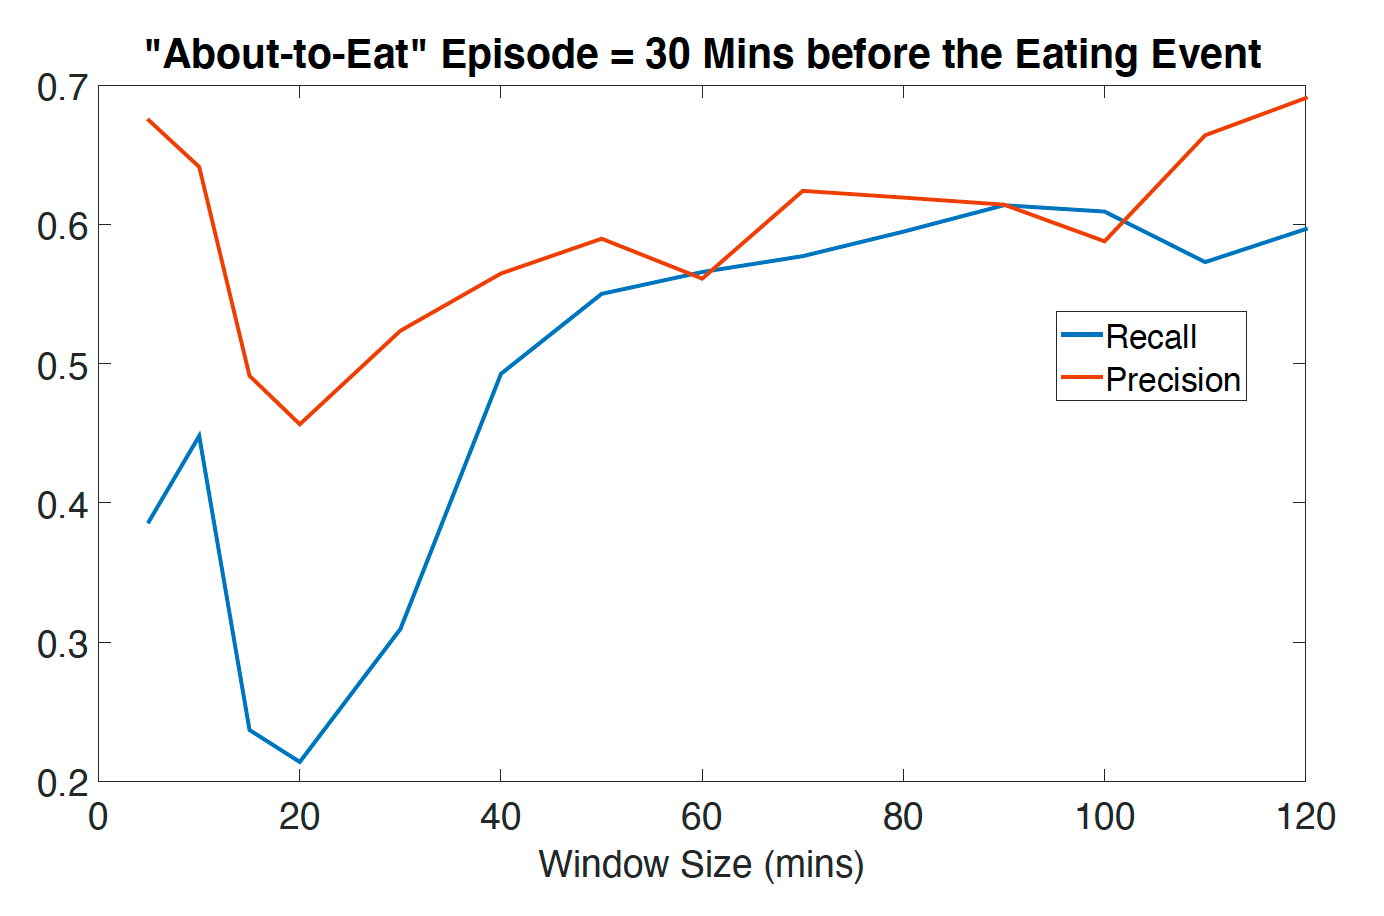
\includegraphics[width=0.5\textwidth]{./images/windowSizePerformance.png}
  \caption{This graph depicts the F measure with the different feature extraction window sizes of the "About-to-Eat" classifier.}
  \label{figure:windowSize}
\end{figure*}

The performance for the "Time until Next Eating Event" model gained a correlation coefficient of 0.49. The most fitting feature extraction window size was assessed, the best performance was reached with a window size of 100 minutes. The authors further claim, that both models could be improved by incorporating person-dependent data from the target user to the models (e.g. person-specific eating pattern, lifestyle).



\textcite{SmartphoneBasedStressPrediction2015}[240, 242-249] research, whether data collected by a user's smartphone can be used to predict stress. In their study, they used an android smartphone app called "TheStressCollector" (TSC) to collect smartphone usage and sensor data in the background. Collected data included: activity, app usage, network traffic, reboot activity (power on and off events), calls (min, max and mean dB-values collected by the microphone), environment brightness, timestamps of received messages, noise exposure, and screen activity. 15 participants installed the app on their smartphone and took part in the conducted study for two weeks. Seven times a day they would fill out questionnaires (at set times), which included the perceived stress score (PSS) and queried them on their current stress status. The stress levels were predicted by WEKA's machine learning algorithms. The mean absolute error (MAE) and Pearson correlation were used for the evaluation. The results of this study presented compelling correlations between PSS and the data collected by the smartphone app. The weekly PSS average, as opposed to the daily one, included the highest correlation coefficient. Thus, it is expected, that it easier to spot longer periods of high stress than shorter ones. This paper is also a team publication featured in the research project from which SmartEater was developed.

In their experiment, \textcite{ClusterPassivelySensedData2018} intend to predict user's negative affect states, in order to provide targeted just-in-time mental health interventions. 65 students participated in the study. Through a smartphone app, GPS location data, accelerometer (activity) data, phone calls, SMS, and ecological momentary assessments (EMA), data was collected and used to cluster participants according to their behavioural profiles. Grouping the participants this way seemed to improve the predictive model's performance.


Other related work: 
\textcite{pius2018automatic} use the k-means clustering algorithm to create automatic annotation of unlabelled smartphone sensor data, to observe sensitive location information of mobile crowd sensing users. \textcite{alcoholCravingPrediction} use smartphone sensor data (e.g. accelerometer) to predict excessive alcohol consumption, in order to replace breathalysers. Their algorithm produced 100\% accuracy, however with 15 minute lags.







% The authors used a variety of different sensors, which at the time, were not all available in one device. The list of utilised sensors and the recorded data are as follows:
% %pages 2,4:
% \begin{itemize}
%   \item Microsoft Band: physical movement (raw accelerometer, gyroscope, step count, speed), caloric expenditure, heart rate, skin temperature, etc. 
%   \item Affectiva Q sensor: measures electrodermal activity (good indicator for psychological arousal) 
%   \item Wearable microphone: chewing and swallowing sounds (for detection of current eating events)
%   \item Android smartphone application: GPS location, recording self-reports (right before eating: "Start of Eating Event" button, current emotional state when eating, intensity of desire/craving and hunger; when finished eating: "End of Eating Event" button)
% \end{itemize}
% Through location traces, physical activity traces (step count, speed, and calorie consumption) and the time of user's gestures/movements (accelerometer and gyroscope)


% In order to train an "About-to-Eat" moment classifier, signal processing and machine learning were used on the sensor streams. The classifier was trained to recognise the two classes "About-to-Eat" and "Not-About-to-Eat". The average recall of this model resulted in a recall, precision and F score of 0.77, 0.67 and 0.69 (respectively).

% According to \textcite{han2011data}[306-307], precision and recall are measures used in classification. Precision describes the exactness (how many of the positive selected items are positive), recall defines the completeness (how many positive items have been correctly selected). The F-score (or F\textsubscript{1} score) is a measure that combines precision and recall (harmonic mean).
%\textcite{AboutToEat2016Rahman}'s



\section{Theory/Literature Review}
\label{section:Theory}
% %(4000 words)
in theory

  \subsection{Data Mining}
  \label{section:TheoryDataMining}
  %DataMiningAndPredictiveAnalytics
%TODO: talk about why data mining and clustering is now so important, since so much data - also mentioned in data mining concepts.. book on page 363
%THERE ARE CASE STUDIES AT THE END OF THIS BOOK
\textcite{DataMiningAndPredictiveAnalytics}[4] declare, that data mining is used to recognise patterns and trends in large amounts of data. \textcite{han2011data}[16-18] explain, that the term "data mining" is a misnomer. A more suitable phrase would be "knowledge mining from data". The word "mining" represents valuable nuggets found within large amounts of raw material. Other names used to describe the same process include: knowledge discovery from data (KDD), knowledge extraction, data/pattern analysis, data archaeology, and data dredging. The discovery of data is an iterative process represented in the following steps: Data cleaning, data integration (combine multiple data sources), data selection (relevant data is extracted), data transformation (into applicable forms for data mining), data mining (discover patterns), pattern evaluation (determine if patterns have a meaning), and knowledge presentation. 
%The following data forms, are typically used for mining: database data, data warehouse data, and transactional data. Other forms include data streams, ordered/sequence data, graph or networked data, spatial data, text data, multimedia data, and the World Wide Web. 
As stated by \textcite{DataMiningAndPredictiveAnalytics}[9-13, 15-16], data mining requires continuous human supervision for quality monitoring and evaluation. Software alone will serve wrong results. Data mining is used for description of patterns and trends, estimation of numerical values, prediction of future results, classification of categorical variables, clustering of similar objects and association of attributes. 

\textcite{DataMiningAndPredictiveAnalytics}[160] describe the two types of data mining methods: \textit{supervised} and \textit{unsupervised}. \textcite{han2011data}[363] interpret supervised learning as \textit{learning by examples}, whereas unsupervised learning is \textit{learning by observation}. \textcite{DataMiningAndPredictiveAnalytics}[160-163] continue, in supervised methods, there is a predefined target variable and the model learns which values of the target variable correspond to which values of the predictor variable. The goal of the unsupervised approach is to find patterns and structure in the inserted variables. Therefore, no target variable is established. Clustering is used in this thesis and further detailed in section \ref{section:TheoryClusterAnalysis}.
%  The experiment in section \ref{section:Experiment} uses unsupervised machine learning to find clusters in the data.

% Clustering is the most prevalent unsupervised method. As reported by \textcite{han2011data}[32], through using unsupervised machine learning, it is possible to detect classes within data. 

% Problems that can occur in data mining methods are data dredging, underfitting and overfitting. 
% As stated in \textcite{DataMiningAndPredictiveAnalytics}[160-163], data dredging is a problem in data mining, that arises when false results develop in data mining due to random variations of data. Cross-validation is used to prevent data dredging, by guaranteeing that the results can be generalised to an independent dataset. 

% Other problems in data mining include underfitting and overfitting. In their paper on attempting to balance underfitting and overfitting, \textcite{van2010process}[87-89] clarify when these can occur. When fitting a model to a log, underfitting or overfitting the model are main problems. Underfitting the model means not fitting the model well enough to the log, therefore allowing too much behaviour which is not present in the log ("anything is possible"). Overfitting has the opposite effect. The model is fitted too well to the log, thus reducing it to another depiction of the log. It therefore only permits the same paths present in the log. These problems can take effect, for example, in a hospital process. Each patient's path of events is most probably unique, two patients are unlikely to have the same process. Hence, the event log is always growing, therefore generalisation is required to avoid overfitting. Likewise, underfitting (allowing all possibilities) should also be averted. 
% \textcite{DataMiningAndPredictiveAnalytics}[164-165] mention, that another way to describe the overfitting/underfitting problem is through the bias-variance trade-off. In figure \ref{figure:biasTradeOff} there are three scatter plots with data points in two different colours, which need to be separated by a line. The first scatter plot depicts a low-complexity separator (e.g. a straight line), which may have some classification errors (\textit{high bias}), however it needn't change much to accommodate new data points. Therefore, it has \textit{low variance}. The second scatter plot illustrates a high-complexity separator (e.g. curvy line that can separate more of the points correctly), which reduces the amount of errors (\textit{low bias}), but has to change a lot when new data points are added. Thus, it has \textit{high variance}. The higher the complexity of the model gets, the bias is reduced, the variance however increases. The third scatter plot shows both a low-complexity separator and a high one, with additional data. While the low-complexity separator can can still classify with little change, the high-complexity one needs to be altered more. The ideal model has neither high bias or variance.

% \begin{figure*}[h]
%   \centering
%   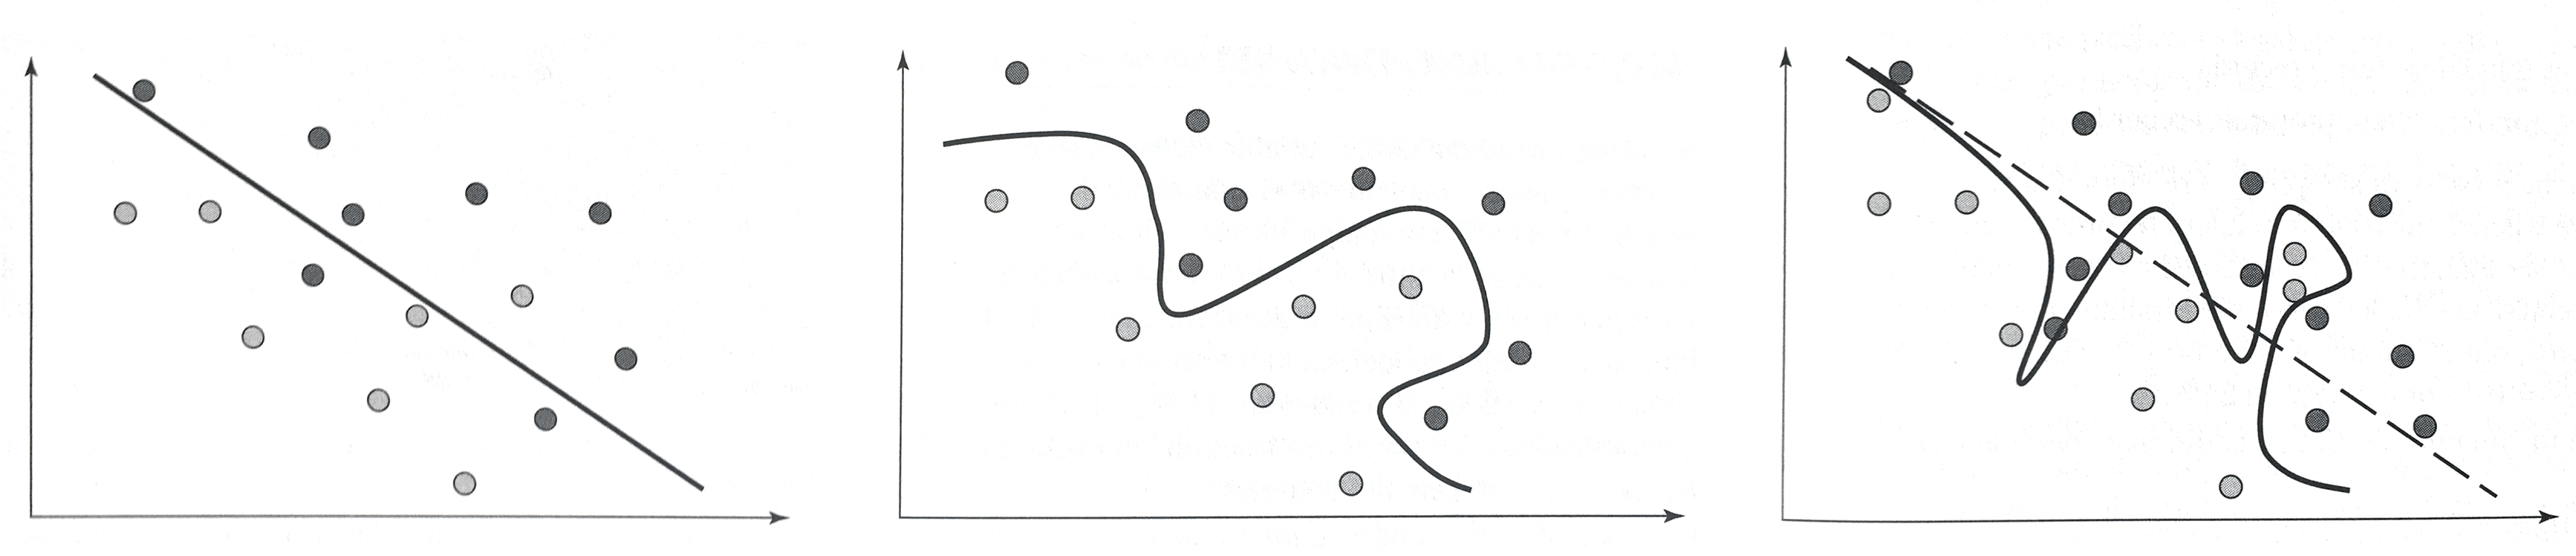
\includegraphics[width=1\textwidth]{./images/biasTradeOff.png}
%   \caption{These three scatter plots from \textcite{DataMiningAndPredictiveAnalytics}[164-165] depict the bias-variance trade-off. The first plot portrays a low-complexity resulting in a high error rate. The second plot achieves a low error rate by using a high-complexity separator. The third graph compares the two separators.
%   }
%   \label{figure:biasTradeOff}
  
% \end{figure*}


%BOOK Data mining concepts and techniques
%page 12 and 13 explains how much data exists, goes through google, basically why we need data mining

%page 18 - another sentence explaining what data mining is, but similar to one from other book
%page 18

%page 28, 29 - outlier analysis

%page 32 - there is an example for unsupervised m. l. on this page, but not really sure if need it

%TODO: EXPLAIN HOW TO NORMALIZE - PAGE 105 OF DATA MINING CONCEPTS.. BOOK -> also explained in data mining and predictive analysis - page 94

%TODO:  data mining concepts and techniques: outlier detection p445, and "Data mining trends and research frontiers" p481
    
  \subsection{Data Preprocessing}
  \label{section:TheoryDataPreprocessing}
  

To make data useful in data mining \textcite{DataMiningAndPredictiveAnalytics}[20] point out, that data sets first need to undergo a data preprocessing step, including data cleaning and data transformation. Raw data extracted directly from databases can be incomplete (values are missing) or be noisy (contains outliers), or may contain out-dated or redundant data. This unpreprocessed data may also not be in a correct form for data mining models. The goal is to decrease garbage in, garbage out (GIGO). Reducing the irrelevant data that is fed into the model (garbage in), the amount of irrelevant data received out of the model is reduced (garbage out).

% \textcite{advancedDataPreprocessing}[] concentrate on data preprocessing to prepare their data to extract users' behaviour on websites.

\textcite{dataPreprocessingInDataMining}[45] outlines dirty data as either missing data or wrong (noisy) data. The sources of these result from data entry errors, data update errors, data transmission errors and bugs. Dirty data can impact the produced model, making it less reliable. The significance of its effect depends on the implemented data mining method.
%TODO: maybe min max normalisation if can't find any other source


\subsubsection{Noisy data}
\textcite{dataPreparationForDataMining}[71-72] interprets outliers as objects that have low recurrence and separated from the main collection of values. These values are often mistakes and can lead to distortion of the data set. Insurance companies provide a good example of outliers. The majority of insurance claims are only for a small sum, however every so often a customer may be in need of a large claim. \textcite{han2011data}[28-29] mention, that in some cases, these uncommon events are of more interest. One of these instances is detecting unusually large payments compared to the card holders normal payments, to uncover fraudulent usage of credit cards.

As stated by \textcite{DataMiningAndPredictiveAnalytics}[26-27], there are some data mining that have trouble functioning correctly when fed outliers. Moreover, outliers may be data errors. Graphical methods used to identify outliers include, histograms or two-dimensional scatter plots. In order to smooth the data, \textcite{han2011data}[84] use binning, regression and outlier analysis (e.g. clustering).

% \begin{itemize}
%   \item Binning: The values are sorted into bins, according to their neighbours. In smoothing by means, each value in the bin is replaced by the bin's mean (or median) value. In smoothing by boundaries, each value is substituted with either the minimum value in the bin, or the maximum, whichever value is closer.
%   \item Regression: 
% \end{itemize}

% \textcite{DataMiningAndPredictiveAnalytics}[38] 
% The Z-score method can be used to numerically calculate outliers. Outliers should not automatically be removed from the data set.



% ------------- MISSING VALUES ---------------
\subsubsection{Missing values}
%81 - PROVIDE THIS PDF - CAUSE CAN'T FIND ACTUAL COPY SO MIGHT BE WRONG PAGE NUMBERs - MAYBE MENTION THE CHAPTERS?
According to \textcite{dataPreparationForDataMining}[81-82, 260, 264, 267] it is good practice to differentiate "empty" values from "missing" ones. Empty values do not have a comparable real-world value. Missing values have underlying values that simply weren't recorded. The author does not recommend ignoring the record with the missing value, since it would mean wasting the data stored in the other fields of that record. These fields may contain relevant information. Substituting the value, means that the record can be used. One of the problems with not having these values, is that this missing information content (e.g. predictive or inferential) could be carried by the pattern. Another problem is how to substitute the missing value, without adding bias to the data set. An inadequately chosen replacement value could distort the data set, by adding data which doesn't exist in the real world. A crucial focus is reserving the relationship between variables.  Substitute values, if not suitable, may disrupt the between-variable variability, thus hiding or distorting patterns in the data. 
\textcite{DataMiningAndPredictiveAnalytics}[23, 25] gives an example, of how replacing missing values can lead to invalid results: The authors experimented with a database of cars. Substituting a missing brand with a random value (here "Japan") led to a car, that doesn't even exist. Data imputation takes into account the other attributes stored in the record and from these, calculates what the missing value would most likely be. Larose D. T. and Larose C.D. suggest, that the value can be replaced, either with a constant determined by the data analyst, with a field mean (for numerical values) or mode (for categorical values), with a random value, or with imputed values based on different features of the record.  
\textcite{dataPreparationForDataMining}[260, 267-269] point out, that regression can be used to find supplement values. Using regression (e.g. linear regression), one can calculate a value, with the help of another given value. There are several different methods to replace missing values, some which promise to generate more information. Such methods are however computationally complex.  


%%for more on data imputation - see chapter 27 

% \textcite{DataMiningAndPredictiveAnalytics}[25] 
% Another step in data preprocessing is identifying missclassifications. An example given by the authors, is classifying a record as USA instead of US, or France instead of Europe. These classes only contained one record in comparison to the other more frequently used classes.

%page 27 - chapter measures of center and spread - not sure if need - mean, median and mode

\subsubsection{Normalisation}

%TODO: ADD GRAPHS, CAN ALSO BE FROM A WEBSITE, E.G. https://www.codecademy.com/articles/normalization

% \textcite{DataMiningAndPredictiveAnalytics}[130-31] 
% In some data mining algorithms, variables with higher ranges can unjustly influence the results, having more influence than smaller ones. Therefore, the authors recommend to normalise numerical data. 

%THIS IS ALSO EXPLAINED BY DATA PROCESSING IN DATA MINING ON PAGE 47
\textcite{han2011data}[105-106] describes normalisation as giving the attributes equal weight. For example, it can transform the data to fall in a smaller, common range (e.g. [-1, 1]). It therefore hinders variables with large ranges from outweighing ones with smaller ranges. For example, income would have a larger range than binary attributes. 

% %data mining concepts and techniques
\textcite{dataPreprocessingInDataMining}[46] explains that raw data is often transformed to produce new attributes with more applicable properties in the process of normalisation. These new attributes are then known as \textit{modeling variables} or \textit{analytic variables}. \textit{Min-Max Normalization}, \textit{Z-score Normalization}, and \textit{Decimal Scaling Normalization} are methods that convert the distribution of the existing attributes.


% \textcite{han2011data}[105-106] 

For the following examples, \textit{A} is a numerical attribute from a data set, a single value of this attribute is represented with \textit{v}:
\begin{itemize}
  \item Min-max normalization scales the original numerical values to a newly defined range, with a new minimum (\textit{newMin\textsubscript{A}}) and maximum (\textit{newMax\textsubscript{A}}) (e.g. 0.0 and 1.0). The original minimum and maximum values found in \textit{A} are presented as \textit{min\textsubscript{A}} and \textit{max\textsubscript{A}} respectively:
  \[
    v' = \frac{v - min_A}{max_A - min_A}(newMax_A - newMin_A) + newMin_A
  \]
  The intervals [0, 1] and [-1, 1] are common intervals for normalisation. 
  % If new data is added, that isn't within the min and max of \textit{A} range, an "out-of-bounds" error will occur.

  \item Z-score (or zero-mean) normalization normalises the values using the mean (\textit{\={A}}) and standard deviation \textit{$\sigma$\textsubscript{A}} of the values \textit{A}.
  \[
    v' = \frac{v - \overline{A}}{\sigma_A}
  \]
  After this transformation, the mean equals zero and the standard deviation is one. The advantage of this normalisation method, is that the min and max values of A do not need to be known, or when there are outliers that could bias the min-max method.

  \item The decimal scaling method moves the decimal point as many spaces, so that the maximum absolute attribute value of \textit{A} is below one. The smallest number of digits that the decimal point has to be moved, so that the largest absolute number in \textit{A} is below zero, is represented by \textit{j}:
  \[
    v' = \frac{v}{10^j}
  \]
\end{itemize}



\subsubsection{Data transformation}
NOT REALLY SURE WHAT TO DO HERE - LEAVE OPEN, WAIT AND SEE WHAT HAVE TO DO IN THE EXPERIMENT
%not sure if should explain these more, page 32 has Decimal Scaling.

%should state the difference between categorical and numerical data - maybe page 333
%page 39-41
As reported by \textcite{DataMiningAndPredictiveAnalytics}[39-41, 45], flag variables can be used to transform categorical variables into numerical. A flag variable can take on one of two values: 0 and 1 (e.g. female = 0, male = 1). When k $\geq$ 3 (k being the amount of categorical predictors), the variables can be transformed into k-1 flag variables. Assigning categorical variables numerical values is not advised, since this orders the categorical variables. For example, if North = 1, East = 2, South = 3 and West = 4, West would be closer to South than to North, etc.


%page 45
ID fields should be removed from the dataset, since the value is different for each record and not helpful.

%OTHER TOPICS - NOT SURE IF NEED:
%page 38- z-score for detecting outliers, like in boxplot
%page 39 - Flag Variables
%page 40 - Transforming categorical variables into numerical variables
%page 41 - Binning numerical variables
%page 56 - exploring categorical variables
%page 64 - exploring numerical variables


% \subsubsection{Something, not sure what yet}



  \subsection{Dimensionality Reduction}
  \label{section:TheoryDimensionalityReduction}
  
\textcite{bellman1957dynamic}[20-22] first introduces the \textit{curse of dimensionality}. The curse effects a mathematical model, when there are a large number of variables. The real world is complex and by trying to incorporate as many real world features into a mathematical model as possible, it becomes complicated. A too simple model however, will not be suitable for prediction. 
\textcite{bellman1961adaptive}[94] further details the results of \textit{the curse of dimensionality}. Functions with one variable can be visualised as curve in a 2D space and a function with two variables in a 3D space. Depicting functions with more variables however, is more problematic (both for visualisation and tabulation). As stated by \textcite{han2011data}[93], dimensionality reduction is a data reduction method. Data reduction is utilised to attain a smaller, more concentrated dataset, whilst mostly keeping the integrity of the initial dataset. Principal components analysis and t-SNE are dimensionality reduction techniques used to reduce the SmartEater dataset.


\subsubsection{Principal Components Analysis (PCA)}
Principal Components Analysis was first proposed by \textcite{OnLinesAndPlanes1901} and \textcite{hotelling1933analysis}.
Pearson's approach is to identify a line or plane that best fits the collected variables plotted to a plane. In order to determine the best fitting line or plane, means, standard-deviations, and correlations are used \autocite{OnLinesAndPlanes1901}[559-560].
\textcite{hotelling1933analysis}[5] introduces his method as the method of principal components. \textcite{jolliffe2002PCA}[7] clarifies, that while these two papers used different methods, the standard algebraic
derivation was announced by \textcite{hotelling1933analysis}. According to \textcite{han2011data}[95-96], the general idea is to calculate k orthonormal vectors, the so called principal components. These unit vectors present a basis for the input data, which are a linear combination of the principal components. \textcite{DataMiningAndPredictiveAnalytics}[94] explain, that the principal components can be discovered, by rotating the initial coordinate system to the direction of maximum variability. These then create a new coordinate system. \textcite{hotelling1933analysis}[4, 5, 15, 18] explains, that the components are chosen with decreasing amount of variance. Therefore, the one with the highest variance is chosen first. The next highest is chosen orthogonal to the one before, and so on. \textcite{han2011data}[93, 95-96] mentions, in data mining, the vectors with the lowest variance are removed, thus reducing the number of dimensions. Despite the loss of data, the components with higher variance can approximate the original data.


\subsubsection{t-Distributed Stochastic Neighbor Embedding (t-SNE)}
\label{section:tSNE}
In their paper, \textcite{maaten2008visualizing}[2579-2580] introduce t-SNE, a method of dimensionality reduction and visualising high dimensional data on a two or three-dimensional plot. The authors mention, that while linear methods like PCA concentrate on making sure low-dimensional representations of data points are apart from each other, they are typically unable to bring similar low-dimensional representations near. 

The authors describe, that t-SNE is a variation of Stochastic Neighbor Embedding (SNE), introduced by \textcite{hinton2003stochastic}. \textcite{maaten2008visualizing}[2581] explain, that the first step in SNE is to transform the Euclidean distances between points in high-dimensional space into the conditional similarity probabilities. According to \textcite{hinton2003stochastic}[2], such a probability \textit{p\textsubscript{i,j}} would arise from the similarity between the two data points \textit{x\textsubscript{i}} and \textit{x\textsubscript{j}}. This is the probability of \textit{x\textsubscript{i}} picking the point \textit{x\textsubscript{j}} as its neighbour. \textcite{maaten2008visualizing}[2581] clarify, that this is the probability of \textit{x\textsubscript{i}} picking the point \textit{x\textsubscript{j}} as its neighbour under the circumstance, that the neighbours were chosen according to their probability density under a Gaussian, \textit{x\textsubscript{i}} being its centre. This results in the conditional probability being high for close data points and imperceptibly small for those further apart.
In a similar way, the conditional probability between the low-dimensional data points \textit{y\textsubscript{i}} and \textit{y\textsubscript{j}} (counterparts to high-dimensional \textit{x\textsubscript{i}} and \textit{x\textsubscript{j}}), represented by \textit{q\textsubscript{i,j}}, is calculated. 
\textcite{maaten2008visualizing}[2581] state, that if the similarity of \textit{x\textsubscript{i}} and \textit{x\textsubscript{j}} has been correctly mapped by \textit{y\textsubscript{i}} and \textit{y\textsubscript{j}}, then \textit{p\textsubscript{i,j}} will be equal to \textit{q\textsubscript{i,j}}. 


\textcite{hinton2003stochastic}[2] further explain, that the goal is to reduce the difference between \textit{p\textsubscript{i,j}} and \textit{q\textsubscript{i,j}}, thus finding a suitable low-dimensional representation of the high-dimensional data. This is accomplished by minimising a cost function, comprised of the sum of the Kullback-Leibler divergences between {p\textsubscript{i,j}} and \textit{q\textsubscript{i,j}}. 
\textcite{maaten2008visualizing}[2583] then list the advantages of t-SNE over SNE are the improvement of its cost function (symmetrised version of SNE) and the use of Student-t distribution as opposed to Gaussian, for the similarity calculation in the low-dimensional area.


To apply t-SNE to a dataset, \textcite{maaten2008visualizing}[2582] describe, the $\sigma$\textsubscript{i} has to be chosen for variance of the Gaussian centred over \textit{x\textsubscript{i}}. Depending on the density, different values of $\sigma$\textsubscript{i} provide better results. For example, in a denser region, a smaller $\sigma$\textsubscript{i} is recommended, but not in less denser regions. This makes it unlikely to be able to find an overall optimal  $\sigma$\textsubscript{i} for the dataset. \textcite{hinton2003stochastic}[2] declare, that $\sigma$\textsubscript{i} can be chosen by hand or is found using a binary search. This would equalise the distribution entropy to log\textit{k}, \textit{k} being the effective number of local neighbours or the so called perplexity. The perplexity is a parameter chosen by the user for the SNE by hand. \textcite{maaten2008visualizing}[2582] imply, that this parameter should be chosen between 5 and 50 and that SNE is quite robust to the chosen value. 
Another parameter to be set is the learning rate. \textcite{han2011data}[332] clarify, that the learning rate parameter is used to support the finding of global minimums, instead of being caught in a local minimum. A learning rate set too low will result in slow learning. In contrast, a learning rate set too high could lead to poor results.


  
  \subsection{Cluster Analysis}
  \label{section:TheoryClusterAnalysis}
  %https://books.google.at/books?hl=en&lr=&id=ZuIPv7OKm10C&oi=fnd&pg=PR5&dq=cluster+analysis&ots=7FXG9i4Yaa&sig=A0WB7hvq7hazTSWkYFrr_3iTAZU#v=onepage&q=cluster%20analysis&f=false



\textcite{hartigan1975clustering}[1] describes clustering as a means to group similar objects together. For example, two planets are considered similar, if (given measurement error) it is probable they could be perceived as the same planet. \textcite{romesburg2004cluster}[2] gives the gathering of a variety of pebbles and sorting them into piles of similar attributes (e.g. shape, size, colour) as an example of cluster analysis. \textcite{hartigan1975clustering}[1-3, 6] further explains, that it can be expected from similar objects for them to act and be treated the same. Clustering is also used to name, display, summarise, predict, and require explanation of the objects in the cluster. If some of the objects assigned to a cluster exhibit certain properties, it is expected that the other objects in this cluster will exhibit them as well. Real-world examples of clustering include classifications of animals, plants and diseases.

\textcite{han2011data}[361-363] state, that the objects placed into one cluster are dissimilar to the objects assigned to other clusters. The fact that cluster analysis can find groups by itself, gives it its unique advantage. Clustering is a type of unsupervised machine learning, since the class label for each group is unknown and needs to be discovered. In data mining, it is utilised to understand the distribution of the data and inspect the distinctions between clusters. Moreover, it can be used to preprocess data for other data mining methods, such as characterisation, attribute subset selection, and classification.
Cluster analysis is used in various fields, including: biology, security, business intelligence, image pattern recognition, and web search. It can be used to place customers into groups, organise projects into categories in project management, and to sort web search results into concise groups. Furthermore, it can be used to detect outliers, since these are located outside of clusters.
%  The detection of outliers is useful in credit card fraud and for identifying criminal activity in e-commerce. 


% According to \textcite{hartigan1975clustering}[9-10], there are usually five different types of variables used in practice in clustering:
% \begin{itemize}
%   \item Counts: no arbitrary scale (e.g. number of legs on a spider) 
%   \item Ratio scale: only defined in proportion to a standard volume (e.g. volume of a liquid in a glass)
%   \item Interval scale: chosen from a standard position in a standard unit (e.g. height of a building)
%   \item Ordinal scale: ordered classification, can be changed by a monotonic transformation (e.g. socio-economic status)
%   \item Category scale: classification that can be adjusted by a one-to-one transformation (e.g. religion)
% \end{itemize}
% A dataset can be comprised of various variable types (\textit{mixed}), of the same type but with different ranges (\textit{heterogeneous}), or of variables with the same range (\textit{homogenous}). There are also methods for conducting type or scale conversions.

%data mining concepts..


% According to \textcite{DataMiningAndPredictiveAnalytics}[524], clustering can also be used to prepare data (create clusters), for example for the input into neural networks.
% \textcite{DataMiningAndPredictiveAnalytics}[524-525] explain, that data should be normalised before being put into a clustering algorithm, thus optimising the performance. Min-max normalization or Z-score standardization can be used to do so (see section \ref{section:Normalisation}).
% TODO:INSERT OTHER EXAMPLES HERE
%TODO: MORE ON OUTLIER DETECTION IN CHAPTER 12







%p 362 2nd to last paragraph - also example on using clustering in image recognition, image of numbers to partition each number into cluster

%TODO: use these sentences?:
% Clustering algorithms are used to create clusters, instead of humans. Consequently, groups of data can be unearthed, that were undiscovered before.

% Distance measures are used to determine the similarities and dissimilarities between objects. 





    \subsubsection{Overview of Clustering Algorithms}
    \label{section:TheoryOverviewClusteringAlgorithms}
    % As stated by \textcite{hartigan1975clustering}[11-12], clustering algorithms search through clusters to find a match for their data. Hartigan classifies the algorithms with the following properties:

% \begin{itemize}
%   \item Sorting:
%   \item Switching
%   \item Joining
%   \item Splitting
%   \item Adding
%   \item Searching
% \end{itemize}

%TODO: ROUSSEEUW 1987 SILHOUETTES page 1: There are many algorithms for partitioning a set of objects into k clusters, such as the - maybe good sources k-means method [6,9,13] and the k-median approach [20].



\textcite{han2011data}[363-365] list the following requirements  clustering methods must meet:
\begin{itemize}
  \item Scalability: clustering algorithms need to work on large databases, which may contain millions or billions of entries.
  \item Ability to work with different attribute types: The algorithm must be able to handle various data types, for example: binary, nominal (categorical), and ordinal data. More complex data types include graphs, sequences, images, and documents.
  \item Recognising clusters with arbitrary shapes: Methods that use distance measures (e.g. Euclidean or Manhattan) to compute clusters usually find clusters of spherical shape. The size and density also tend to be similar. Clusters could however be of any shape, therefore the algorithms need to be capable of detecting any shape.
  \item Requirements for domain knowledge: For some clustering algorithms, parameters (e.g. desired number of clusters) need to be determined. These can affect the cluster results. Parameters are hard to define, if the data is not understood.
  \item Ability to handle noise (see section \ref{section:NoisyData})
  \item Incremental clustering: The method should be able to integrate incremental data updates into existing structures, without recomputing the clustering.
  \item Insensitivity to the order of the input: The clustering results should be the same, regardless of the order the objects are inserted into the algorithm.
  \item Ability to cluster high-dimensional data (see section \ref{section:TheoryDimensionalityReduction}) %there is quite a good explanation here, but not really sure if need it
  \item Capability to cluster under certain constraints %TODO: do i need an example constraint? not explained very well in the book
  \item Interpretability and usability of the results
\end{itemize}

% TODO: ON PAGE 356 - THERE ARE TECHNIQUES ON HOW TO COMPARE CLUSTERING METHODS - NOT SURE IF NEED

%TODO: check if all pages have been used - have been highlighting lines that have used
%TODO IMPORTANT: this might not be 366-296 - depends on if i end up explaining in more detail - at end, find which pages i actually used


\textbf{todo: add images to compare how different methods cluster}
\textcite{han2011data}[366-396] present different clustering algorithms. They state, that it is not easy to divide these into distinct categories, since some algorithms share features from other categories. The general categories are partitioning methods, hierarchical methods, density-based methods and grid-based methods.

(\textbf{Todo: Explain used methods in more detail after Experiment and add figures of graphs})
% \textbf{TODO: ONLY EXPLAIN IN DETAIL, WHICH METHODS ARE USED IN THE EXPERIMENT}
%TODO:maybe also look into performance comparisons
  \subsubsection{Partitioning Methods}
  Partitioning methods are the easiest and most significant types of clustering methods. The data is divided into \textit{k} (generally pre-defined) number of groups (clusters). The data consists of \textit{n} objects, thus \textit{k $\geq$ n}. Each group must contain at least one object. A data object can only be classified into one group (\textit{exclusive cluster separation}). Fuzzy partitioning methods relax this condition.
  Many of the partitioning methods use distance measures to calculate their clusters. If the number of clusters (\textit{k}) is pre-defined, then the clustering algorithm will create an initial segregation into \textit{k} clusters. Objects are then relocated to improve the partitioning. The partitioning is considered good, when objects assigned to the same cluster are "similar" and "dissimilar" from the objects in the other clusters. Traditional partitioning methods can also be applied onto subspaces (for many attributes and sparse data). 
  %Sentence directly copied from book p366, not sure whether to add (needs changing): There are various kinds of other criteria for judging the quality of partitions. - WHICH ARE MENTIONED LATER IN SECTION???
  
  Examples: k-means, k-medoids



  \subsubsection{Hierarchical Methods}
  %CAREFUL!, sentence from book is similar:  A hierarchical clustering method works by grouping data objects into a hierarchy or “tree” of clusters.
  The data is grouped into a hierarchy ("tree") of clusters. Depending on how the hierarchical decomposition is constructed, there are two different approaches: \textit{agglomerative} or \textit{divisive}. In the \textit{agglomerative} or \textit{bottom-up} approach, each object creates its own cluster. Step by step it is then merged into its closest neighbours until all objects belong to one cluster, or a termination condition comes true. In the \textit{divisive} or \textit{top-down} approach, all objects initially form one cluster together. Step by step, each cluster is divided, until each object is contained in its own cluster, or a condition is met to terminate the process. Once a merge or split step has been performed, it cannot be reversed. Once merged/split, the objects also cannot swap cluster. Each merge or split decision influences the quality of the resulting clusters and must therefore be well chosen. Hierarchical methods can be used in subspaces and can use distance measures, or can be density- and continuity-based.

  % todo COULD GO MORE INTO DETAIL ABOUT AGGLOMERATIVE AND DIVISIVE CLUSTERING, SEE PAGES 375-377 - but not sure if need, depends if being used

  Examples: BIRCH, Chameleon
%TODO: PAPER BOOK PAGE 526 - quite interesting- linkage (how to determine distance between clusters)
  %TODO: CHECK, I THINK PARTITIONING AND HIERARCHICAL DON'T FILTER OUT NOISE AND OUTLIERS, BECAUSE THEY PARTITION THE ENTIRE DATA SET, SO EVERY OBJECT IS IN A CLUSTER. WOULD BE GOOD TO MENTION
  

  \subsubsection{Density-Based Methods}
  The majority of clustering methods (e.g. partitioning and hierarchical methods) use distance-based approaches, which results in only finding clusters with spherical shapes. Density-based methods have the ability to find clusters with random shapes. In these methods, objects are continuously added to the cluster, so long as the number of objects/data points (density) close by is larger than a given threshold. The clusters are comprised of high-density areas of objects. These are separated by spaces with low-density. Accordingly, this method is also useful for removing noise and outliers.
  These methods can also be used to cluster sub spaces.

  Examples: DBSCAN, OPTICS, DENCLUE
  %TODO: page 385 - good figure of density based clustering - however might be better to fetch from a paper.



\paragraph{DBSCAN}
\textcite{DBSCAN}[226-229] introduce a new density-based clustering algorithm, the Density Based Spatial Clustering of Applications with Noise. This method is able to find clusters no with different shapes and work efficiently on large spatial datasets. The algorithm searches in a give radius (Eps = epsilon parameter) around a data point. If within this radius a minimum number of points (MinPts parameter) exist, then this point is added to the cluster (core point). A data point (\textit{p}) is considered a border point, if inside of the Eps neighbourhood there is a core point (\textit{q}). A data point is labelled as noise, if it does not belong to any clusters (has no core points within the given radius).
% The goal is to keep adding neighbouring data points to the cluster
% In doing so, core points and border points are distinguished.
%todo: rewrite - that uses two global parameters instead of one - or say that only with one paramter
According to \textcite{han2011data}[388], a weakness of DBSCAN is the fact that the results rely on the chosen parameters. If these are selected differently, the clustering results can differ. These parameters can often be challenging to select.

\textcite{DBSCAN}[230] supports the selection of the Eps and MinPts parameters.



\paragraph{OPTICS}
\textcite{han2011data}[388] mentions, that OPTICS was created to improve the selection of global parameters problem in DBSCAN.
\textcite{OPTICS}[49, 51-] present the density base clustering algorithm OPTICS (Ordering Points To Identify the Clustering Structure). This method in itself does not specifically create clusters. Instead, it orders the data set according to its density-based clustering structure. For each object, the values \textit{core-distance} and \textit{reachability-distance} are calculated. The \textit{core-distance} of an arbitrary data point (object) \textit{o} is the distance to the nearest point within Eps that completes the MinPts rule and therefore labels point \textit{o} as a core point. If there is not the number of MinPts in the Eps neighbourhood, then the \textit{core-distance} of that point is undefined. The \textit{reachability-distance} of an object \textit{p} to core object \textit{o}  is defined as the max value of the core-distance and the distance from object \textit{o} to object \textit{p}. Likewise, if \textit{o} is not a core object, then the {reachability-distance} of \textit{p} is undefined. The \textit{core-distance} and \textit{reachability-distance} are visualised in figure \ref{figure:reachabilityDistanceOPTICS}.

\begin{figure*}[h]
  \centering
  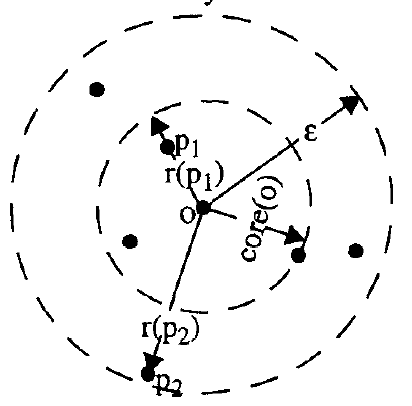
\includegraphics[width=0.3\textwidth]{./images/reachabilityDistanceOPTICS.png}
  \caption{Core-distance of object \textit{o} (MinPts = 4) and reachability-distances for objects \textit{p1} and \textit{p2} \autocite{OPTICS}[52].}
  \label{figure:reachabilityDistanceOPTICS}
\end{figure*}

%TODO: i wrote this from the paper - not sure whether to add - end is missing - see optics page 53 - pseudo code explanation
%The OPTICS algorithm takes an arbitrary core point, and orders its directly density-reachable objects (according to Eps and MinPts) and sorts them by their reachability-distance (to the selected core point). From the smallest to the largest reachability-distance, each point is selected and added to an OrderedFile, along with its calculated core-distance and reachability-distance.

The data points are ordered by the OPTICS algorithm (using their reachability-distance) to create a reachability plot. This plot is relatively stable towards the input parameters. In figure \ref{figure:reachabilityPlotOPTICS} a reachability plot calculated from a 2D data set is depicted. 

\begin{figure*}[h]
  \centering
  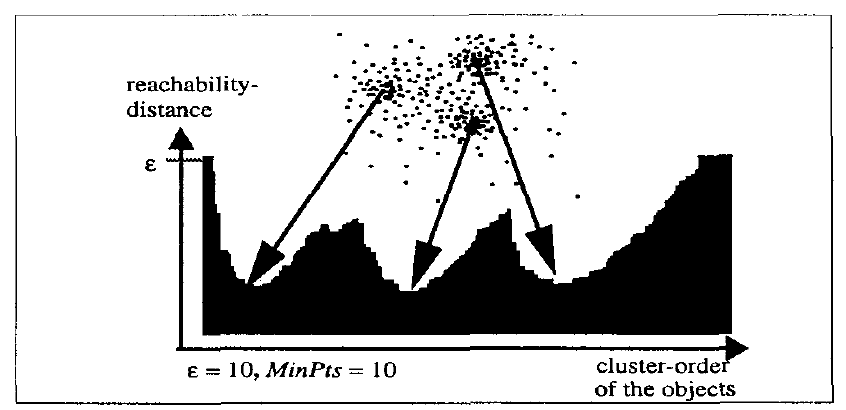
\includegraphics[width=0.5\textwidth]{./images/reachabilityPlotOPTICS.png}
  \caption{OPTICS reachability plot for a 2D data set. Three "Gaussian bumps" can be seen \autocite{OPTICS}[54].}
  \label{figure:reachabilityPlotOPTICS}
\end{figure*}

The clusters can then be automatically constructed from the reachability plot by pinpointing the start-of-cluster and end-of-cluster regions and combining regions that match into clusters (or nested clusters). Since the reachability-distance of a point is the distance from the set of its predecessors and through OPTICS' specific ordering, the clusters are the dips in the reachability plots (as can also be seen in figure \ref{figure:reachabilityPlotOPTICS}). In figure \ref{figure:clusterExtractionOPTICS}


\begin{figure*}[h]
  \centering
  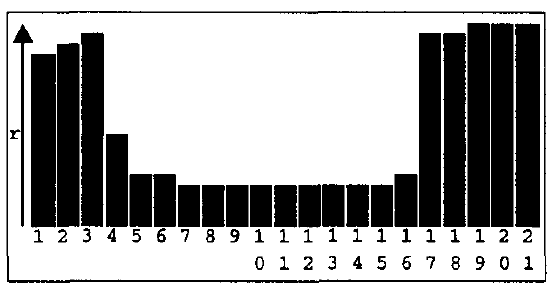
\includegraphics[width=0.5\textwidth]{./images/clusterExtractionOPTICS.png}
  \caption{Since clusters are defined as the dips/dents in the reachability plots create by the OPTICS algorithm, a cluster can be extracted from this plot starting at the 3rd data point and ending with the 16th. The x-axis of the reachability plot depicts the order of the data points (objects) and the y-axis the reachability-distance for each datapoint \autocite{OPTICS}[57].}
  \label{figure:clusterExtractionOPTICS}
\end{figure*}

%todo: In comparison to DBSCAN - problem with containment - optics page 52

 

  \subsubsection{Grid-Based Methods}
  %not sure if correct - sentence from book page 367: The main advantage of this approach is its fast processing time, which is typically independent of the number of data objects and dependent only on the number of cells in each dimension in the quantized space.
  The previously mentioned clustering methods are data-driven (they accommodate the distribution of the data objects). Grid-based methods are space-driven (they do not rely on the distribution of the data objects). The data objects are quantised into grid cells on a multiresolution grid. The actions required for clustering are performed on the grid structure. The processing time depends on the grid size (number of cells) in each dimension and not on the number of objects and is more accelerated than other clustering methods.
  
  Examples: STING, CLIQUE

  \vspace{5mm} %5mm vertical space
\textcite{han2011data}[414, 416] clarify, that the clustering methods mentioned above have a good functionality when used on a data set with fewer than 10 attributes. Another way to cluster high-dimensional data is \textit{subspace clustering}, in which subspaces (subset of attributes) are investigated to find clusters. The CLIQUE method is used for subspace clustering. 


  %TODO: paper book page 542 - kohonen networks

    \subsubsection{Evaluating Clustering Results}
    \label{section:TheoryEvaluatingClusteringResults}
    The resulting clusters received from the previously mentioned clustering algorithms are assessed in the \textit{cluster evaluation} step. \textcite{han2011data}[396, 398] describe this stage as assessing the quality of the results.
There are different steps to be taken in evaluating clusters, e.g. evaluation of the cluster quality, assessment of the cluster tendency (whether non random stuctures exist), and establishing the number of clusters (e.g. for k-means clustering). The experiment described in this thesis used mathmathical evaluation methods to compare cluster quality among the different time lengths. 
 
  % \subsubsection{Assessment of the cluster tendency}
  % As explained by \textcite{han2011data}[396-397], the tendency must be assessed, meaning it is tested, whether structures exist that aren't random. Running a clustering algorithm on any dataset will return clusters. However, only non random structures are significant and not misleading. For example, if a dataset consists of data points that are uniformly distributed, if a clustering algorithm delivers clusters, these will be random and have no purpose. Spatial randomness tests (e.g. Hopkins Statistic) can be used to measure how likely the data was created by uniform data distribution.

 

  % \subsubsection{Evaluation of the cluster quality}
  % (\textbf{Todo: adjust to the methods used in the experiment})

  \textcite{han2011data}[399, 401] mention, that the cluster quality needs to be evaluated. Generally, there are two ways to measure the quality of clustering: extrinsic methods and intrinsic methods. In extrinsic methods, there is a ground truth available, therefore these are also referred to as supervised methods. This ground truth is usually produced by experts (humans). Intrinsic methods are used, when there is no ground truth available. In intrinsic methods, the clusters are evaluated by how well they are separated from one another and how compact they are (e.g. \textit{silhouette coefficient}).
  % NOT SURE IF SHOULD EXPLAIN EXTRINSIC, SINCE DON'T THINK USING.
  The experiment described in this paper uses intrinsic methods, since there is no ground truth for comparison.
  
  
  \paragraph{Silhouette Coefficient}
  \label{section:silhouetteCoefficient}
  In his paper, \textcite{rousseeuw1987silhouettes}[53-57, 59] proposes a new graphical display using silhouettes, to help determine how well objects belong to their assigned clusters. It can be used to interpret and validate the results of clustering. It is also utilised to compare the resulting clusters with those output using alternative algorithms (the input data being the same). 
  
  % In an example, where countries are assigned a value of how dissimilar they are to another country, the results are listed in a table. A structure contained in the results (consisting of 66 numbers), is hard to identify. Therefore, the countries are categorised into clusters using k-median. It is however uncertain, whether the clusters follow a specific structure, or if the groups are simply artificial. 
  % With the use of silhouettes, the author's goal is to answer the following questions: Is the quality of the clusters high, therefore the dissimilarities of the objects within a cluster are small, and large compared to the objects in other clusters? Are the objects well-classified, misclassified and which ones were not classified (between clusters)? Is it possible to perceive which "natural" clusters are available in the dataset?
  %According to Rousseeuw, the silhouettes are ideal when the distance between objects are on a ratio scale (e.g. Euclidean distances) and when the goal is to receive clear and compact clusters.

  The formula is as follows:
  With the use of silhouettes, the author's goal is to find out, if the quality of the clusters is high. Hence, the dissimilarities of the objects within a cluster are small, and the dissimilarities are large compared to the objects in other clusters. For each object \textit{i} (in cluster \textit{A}) the value \textit{s(i)} is calculated. \textit{a(i)} contains the average dissimilarity of the object \textit{i} to each other object in the same cluster. If there are no other objects in the cluster, \textit{s(i)} is set to zero (most neutral value). \textit{b(i)} is determined by firstly calculating the average dissimilarity for each neighbouring cluster that isn't \textit{A}. The shortest of these values, therefore the next closest cluster to \textit{A}, is then assigned to \textit{b(i)}. This cluster can so to say be seen as the next best choice for \textit{i}. \textit{b(i)} can only be calculated, if there are other clusters beside \textit{A}. The formula for \textit{s(i)} is as follows:
  \[
    s(i) = \frac{b(i) - a(i)}{max\{a(i), b(i)\}}  
  \]
  The resulting value \textit{s(i)} is a number in the range of \textit{-1 $\leq$ \textit{s(i)} $\leq$ 1}:

  \[ s(i) =
  \begin{cases}
    1 - a(i)/b(i)       & \quad \text{if } a(i) < b(i)\\
    0       & \quad \text{if } a(i) = b(i)\\
 b(i)/a(i) - 1      & \quad \text{if } a(i) > b(i)

  \end{cases}
\]
A \textit{s(i)} value close to 1 reveals, that the dissimilarity within a cluster is smaller than the dissimilarity to the neighbouring cluster. Therefore it suggests, that the assignment of that object is good, since it is most likely the most suitable cluster for \textit{i} (well-classified). A \textit{s(i)} value close to 0 means that \textit{a(i)} and \textit{b(i)} are almost equal and it is uncertain whether cluster \textit{A} or its neighbour is a more suitable fit. If \textit{s(i)} is near -1, then the dissimilarity within a cluster is larger than the dissimilarity to the next closest cluster. Thus, it would have been more natural to assign \textit{i} to the neighbouring cluster, since it is closer to it (misclassified).

The \textit{average silhouette width} can be calculated for single clusters. It is received by calculating the average of all objects that belong to said cluster. An average score can also be calculated from each object \textit{i} for the whole chart (dataset), the so called \textit{overall average silhouette width}. 

% \textcite{silhouetteRelocatingMeasure}[15] use the silhouette coefficient in their proposed clustering algorithm, which clusters categorical data. The coefficient was used assess the quality of the clusters and to relocate objects to more fitting clusters. The cluster efficiency in their algorithm was therefore enhanced.



% %TODO: there is some more about it with examples - but not sure if need - from p. 584

\paragraph{Davies-Bouldin Index}
A second cluster evaluation method is the Davies-Bouldin Index, which was announced by \textcite{DaviesBouldin}[224-227]. 
% The goal is to calculate the average similarity of a cluster with the cluster that is most similar to it. 

The succeeding formula describes the average similarity of a cluster with the cluster that is most similar to it (\textit{R\textsubscript{ij}} ).
\textit{i} and \textit{j} represent the determined clusters, \textit{S\textsubscript{i}} and \textit{S\textsubscript{j}} stand for the dispersions of the clusters, and \textit{M\textsubscript{ij}} is the distance between the two cluster centroids. 

\[
  R_{ij} = \frac{S_i + S_j}{M_{ij}}  
\]

The Davies-Bouldin Index equals:
\[
\overline{R} = \frac{1}{N}\sum_{i=1}^{N}R_i
\]

This metric can be used, to compare clustering results. The lower of the two \textit{\=R} values indicates the better partitioning.

\paragraph{Caliński-Harabasz Index}
As a third evaluation score, \textcite{calinskiHarabasz}[3, 7, 11, 23, 24, 26] is used to evaluate and compare the resulting clusters in the experiment. 
The Caliński-Harabasz Index or Variance Ratio Criterion (VRC) is calculated as 
% follows, where \texit{n} is the number of points \textit{k} is the number of clusters, \textit{WGSS} is the within-group (cluster) sum of squares, and \textit{BGSS} is the between-group (cluster) sum of squares.
\[
VRC = \frac{BGSS}{k-1}/\frac{WGSS}{n-k}
\]
If \textit{k} is not known, it is set to 2, then 3 and so on. The density of the clusters can be calculated with the sums of the squared distances from the cluster centroids, to the points. The more natural the clusterings are, the higher VRC will be, since the variation within the cluster is lower.


%Determining the minimum of WGSS can be utilised for cluster analysis.



% \subsubsection{Establishing the number of clusters}
%  \textcite{han2011data}[398] states, that the number of clusters (\textit{k}) found in the dataset needs to be established. For some clustering methods (e.g. \textit{k}-means), this number is defined before the clustering process. This number can be challenging to determine and depends on the shape and scale of the input data. A good number of clusters creates a balance between \textit{compressibility} and \textit{accuracy}. Having only one cluster would have maximum compression, but no value. Contrarily, if each data object formed its own cluster, the clusters would be most accurate, but not allow for summarisation of the data. 
% \textcite{rousseeuw1987silhouettes}[59] describes, how silhouettes can be used to determine the ideal amount of clusters. Picture a dataset with dense clusters which each have large distances to the other clusters. When \textit{k} is chosen too small, naturally occurring clusters must be artificially joined, to satisfy the value \textit{k}. Implementing the silhouette calculation will result in high within-cluster dissimilarities (\textit{a(i)}) leading to a narrow silhouette (small \textit{s(i)}). Likewise, if \textit{k} is chosen too large, natural clusters will have to be artificially split, in order to gain \textit{k} clusters. The objects in a split natural cluster will however still be very close to the other half of their cluster, therefore resulting in low dissimilarities between clusters (\textit{b(i)}) and a small \textit{s(i)}.
% This logic denotes, that silhouettes should be capable of finding the most 'natural' number of clusters in a dataset.


  

  \subsection{Data Visualisation with t-SNE}
  \textbf{Todo: if used in the experiment}



\section{Experiment/Method?}
\label{section:Experiment}


The goal of this paper is to identify, which time delta for aggregation is ideal to construct distinct clusters from smartphone sensor and usage data. The data for this experiment was collected for the upcoming SmartEater \footnote{\url{https://sites.google.com/site/eatingandanxietylab/resources/smarteater} (last visited 27. June 2020, 19:40)} mobile health app. The goal of this app is to present the user with content-dependent feedback, with the hope to prevent food craving episodes. By evaluating the user's behaviour (through smartphone sensor and usage data), the app predicts eating crises through stress, therefore eliminating the need of intense user input. 

Various sensor and usage data was recorded for the SmartEater project, by the 46 testers' smartphones (for different periods of time). The columns of the data were organised as follows (N is the number of times the data was recorded in the time period and app usage is in percent of lag-interval minutes):
 

\begin{itemize}
	\item TIME: timestamp, when the data was aggregated (format: YYYY-DD-MM hh:mm:ss)
	\item ACC (1-N): values received from the accelerometer (average jerk). According to the Android developers documentation\footnote{\url{https://developer.android.com/guide/topics/sensors/sensors_motion}}, the accelerometer (acceleration sensor) records the acceleration (including the force of gravity) enforced onto the smartphone. 
	\item AUDIO (1-N): volume of the audio 
	\item SCRN (1-N): percentage of screen-on-time
	\item NOTIF (1-N): number of notifications
	\item LIGHT (1-N): (environment) light sensor values
	\item APP\_COM (1-N): app usage in the category \textit{communication} 
	\item APP\_VID (1-N): app usage in the category \textit{video players}
	\item APP\_OTHER (1-N): app usage of all other categories (excluding \textit{video players} and \textit{communication})
\end{itemize}


The recorded smartphone sensor and usage data was aggregated into multiple .csv (Comma-Separated Values\footnote{\url{https://tools.ietf.org/html/rfc4180}}) files. Furthermore, these files were distinguished into folders, according to their time delta. Two different time lengths were used:

\begin{itemize}
  \item 1h: The data was aggregated in 2.5 hour intervals, whereby each row contained data from an aggregation of 1 hour, in four 15 minute lags.
  \item 3h: The data was aggregated in 1.5 hour intervals, whereby each row contained data from an aggregation of 3 hours, in six 30 minute lags.
\end{itemize}

Each row contains the data value of a specific test user for one of the time periods (e.g. 1h or 3h).

Python was used to conduct the experiment, more specifically using the Anaconda\footnote{\url{https://www.anaconda.com/}} Python distribution platform for data science. The scikit-learn\footnote{\url{https://scikit-learn.org/stable/index.html}} (short sklearn) Python package provides simple tools for predictive data analysis and was used for data preparation, dimensionality reduction, and clustering.



  \subsection{Preparation of the Data Set}
  \label{section:ExperimentPreparationDataSet}
  Initially, the raw data in the .csv files was distributed in multiple files (one file per user, per time interval). The files were read in and processed by the Python Pandas\footnote{\url{https://pandas.pydata.org}} tool. The library offers fast and flexible functionalities for data analysis. It utilises DataFrames which are fast and efficient 2D data structures, used to store tabular data. Using the Pandas read\_csv and concat methods, the files with identical time periods were transformed and concatenated to one collective DataFrame. 


\subsubsection{Missing Values}
The raw data contained several rows with empty cells. Section \ref{section:MissingValues} lists approaches on how to substitute missing data, thus preserving the row, which could otherwise contain important information. In doing so however, the existing patterns could be disrupted. In order maintain the data's patterns, rows with missing values were removed. Using the Pandas' dropna\footnote{\url{https://pandas.pydata.org/pandas-docs/stable/reference/api/pandas.DataFrame.dropna.html}} function (deletes rows with missing values), all rows containing empty cells were dropped. Of the original 8283 rows from the 1 hour time period files, only 3279 (39.59\%) rows were complete and remained. In the 3 hour files, only 6218 from 14091 (44.13\%) persisted.

\subsubsection{Normalisation}
The data recorded from the different smartphone sensors returned values with different ranges. For example, whilst the values that describe the screen on time ranged between -20 and 2.0, the light sensor values could reach from 0 to over 60,000. As explained in \ref{section:Normalisation}, values with higher ranges can inadvertently outweigh smaller values. To be sure that the values are weighted the same, \textit{Min-Max Normalization} was used to map all the values into the common range, e.g. [0,1]. The sklearn MinMaxScaler was initially used to calculate the new, normalised values in the data set. Most of the values in the data set ranged between 0 and just over 100. The light sensor values were the exception, with its values reaching above 60,000. As mentioned in section \ref{section:Normalisation}, Z-score normalization is more robust to outliers, that could otherwise bias Min-Max Normalization. Therefore, the sklearn StandardScaler was used instead of the MinMaxScaler, which implements the Z-score normalization.

\subsubsection{Selection of columns (attributes)}
% TODO:
% Also - compressing 1-N columns
In order to only use meaningful data to receive significant results, it was important to remove columns that do not contain any predictive content. The TIME column was removed for this reason. Since the TIME column only showed the time and data when the data was recorded periodically (in fixed intervals), it was \textbf{serial ???????} data that had no influence on the data or any predictive value (like an index). It could have however bias the results if left in. 

To reduce the number of dimensions (number of columns), columns with the same feature (e.g. ACC1-N) were compressed to one column. Each unique feature only requires one column, and therefore reduced the number of columns to only 8 (instead of 32 in the 1h data set or 48 in the 3h data set).


\subsubsection{Chain shaped data}
Initial visualisations of the data set (with t-SNE dimensionality reduction) showed a chain formalisation of the data. This chain can be seen in figure \ref{figure:tsneChain} (light blue data points). A similar accumulation of data points, though this time shaped as a line, can further also be seen in the PCA dimensionality reduced data set (see figure \ref{figure:pcaChain}). 


\begin{figure*}[h]
  \centering
  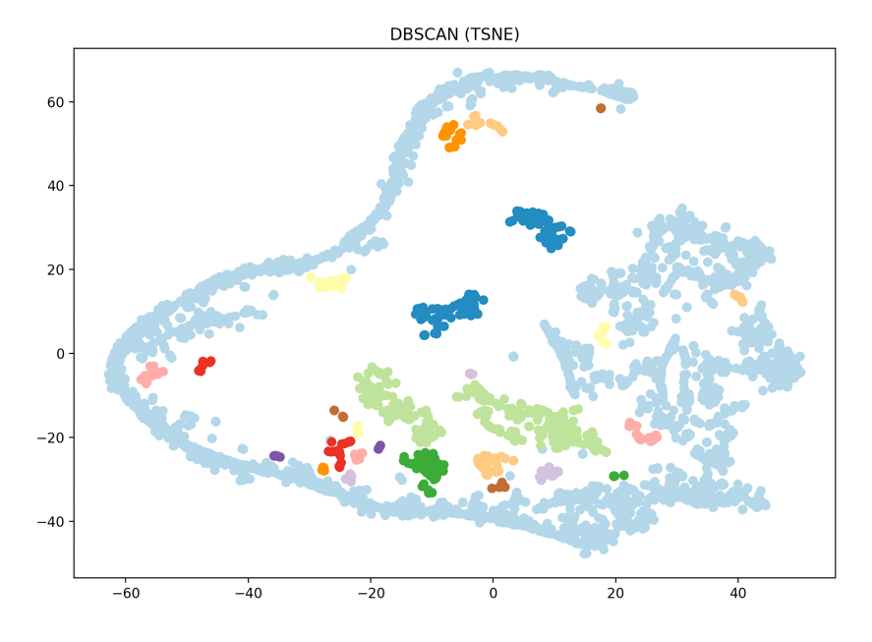
\includegraphics[width=1\textwidth]{./images/tsneChain.png}
  \caption{1h data set, a chain of data points (light blue points) can be seen in the data set.}
  \label{figure:tsneChain}
\end{figure*}


\begin{figure*}[h]
  \centering
  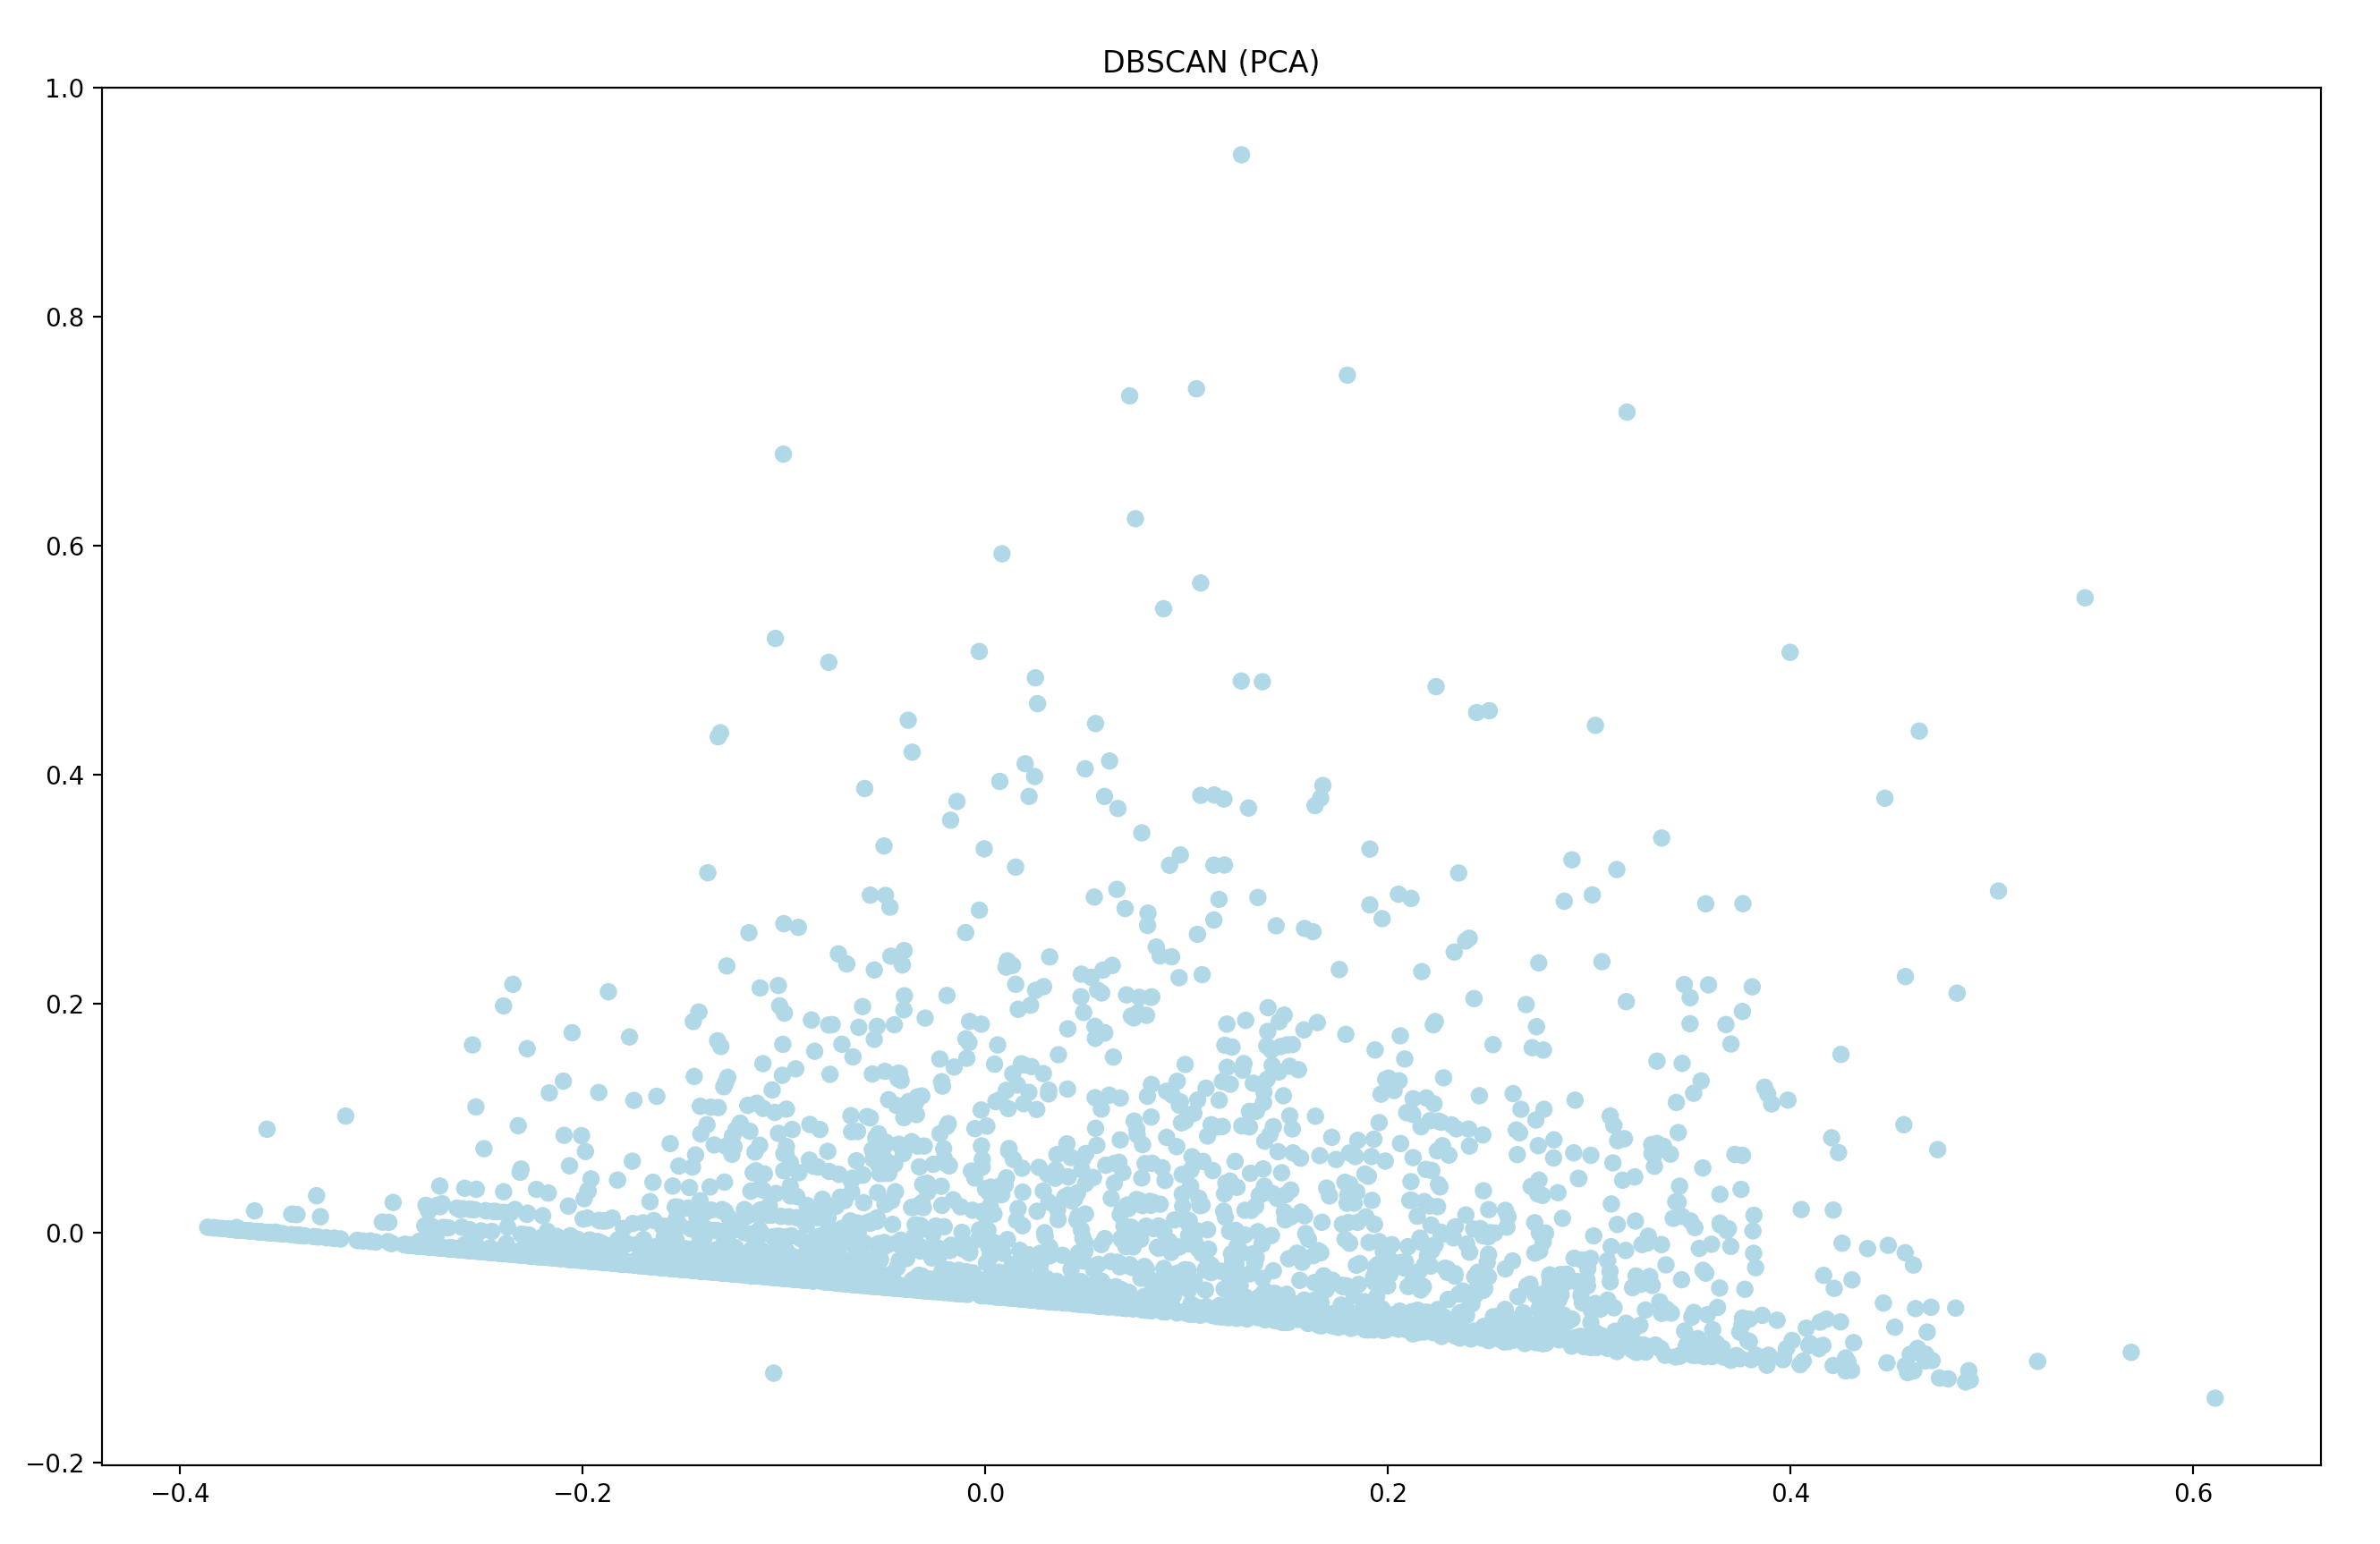
\includegraphics[width=1\textwidth]{./images/pcaChain.png}
  \caption{There is a collection of points along a line. This same collection can also be visualised as a chain in the t-SNE data set.}
  \label{figure:pcaChain}
\end{figure*}

An initial thought, was that this chain was the result of the utilised t-SNE parameters. However, even with changing the t-SNE perplexity, learning rate and number of iterations parameters, the chain persisted in some form. Another thought, as to where these data points originated from or why they resulted in a chain, was that there were dependencies within the data or columns. For example the three APP columns, these indicate the percentage of time in a lag-interval that a type of app was used. Therefore, if say a communication app was used 100\% of this time, the APP\_COM cell for this time would be 1. By using this app for 100\% of the time, would mean that the values in the other APP columns for this time would have to be 0 (0\%), since they would not have been able to be used. To test this theory, the APP columns were removed from the data set and the 2D scatter plot was recalculated. The chain was still visible. Step by step each column was removed, to see if it was the cause of the chain. The chain did not disappear though, which indicated, that the problem was not due to the columns, but rather the rows. The chain was less visible when reducing the number of inserted .csv files (lower number of records) to 10 (see figure \ref{figure:tsne10Files}). When the number of features were reduced to only AUDIO and ACC (two columns), the chain was once again visible (see figure \ref{figure:tsne10Files2Features}). The presumption is that when there are less data points and more features (e.g. 10 files but using all the features), there are enough different data points and the chain less dense, making it less noticeable. When there are less data points but with less features (e.g. 10 files but using only 2 features), or when there are many data points even with multiple features (e.g. all data files and all the features), there are more rows with very similar of equal values and the chain appears more dense and prevalent.

\begin{figure*}[h]
  \centering
  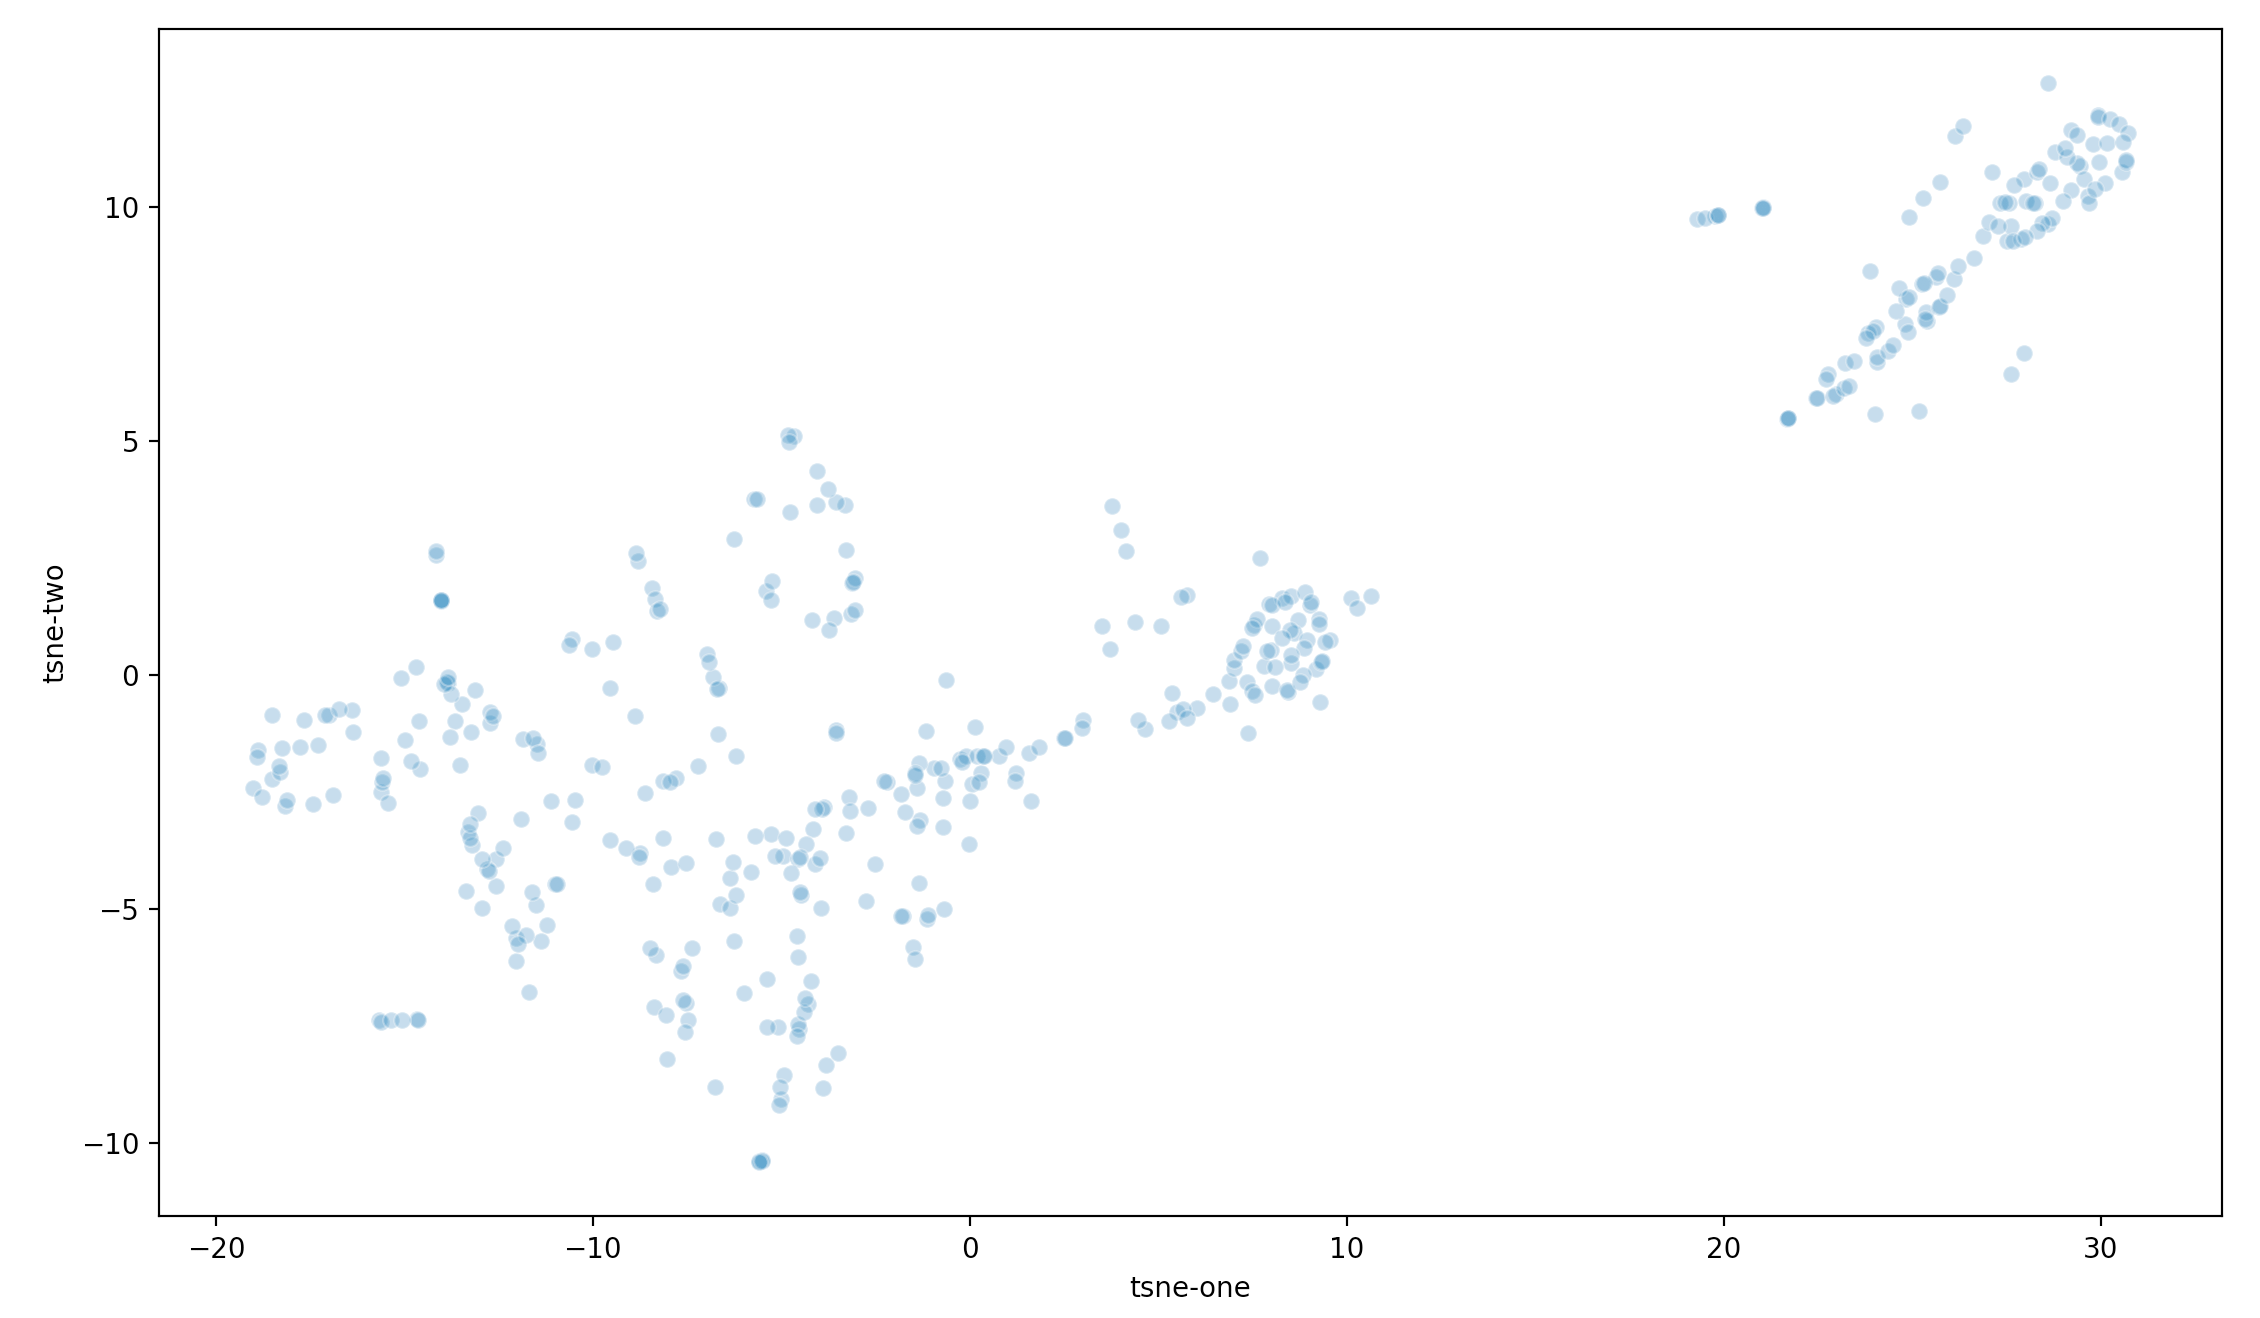
\includegraphics[width=0.5\textwidth]{./images/tsne10Files.png}
  \caption{}
  \label{figure:tsne10Files}
\end{figure*}

\begin{figure*}[h]
  \centering
  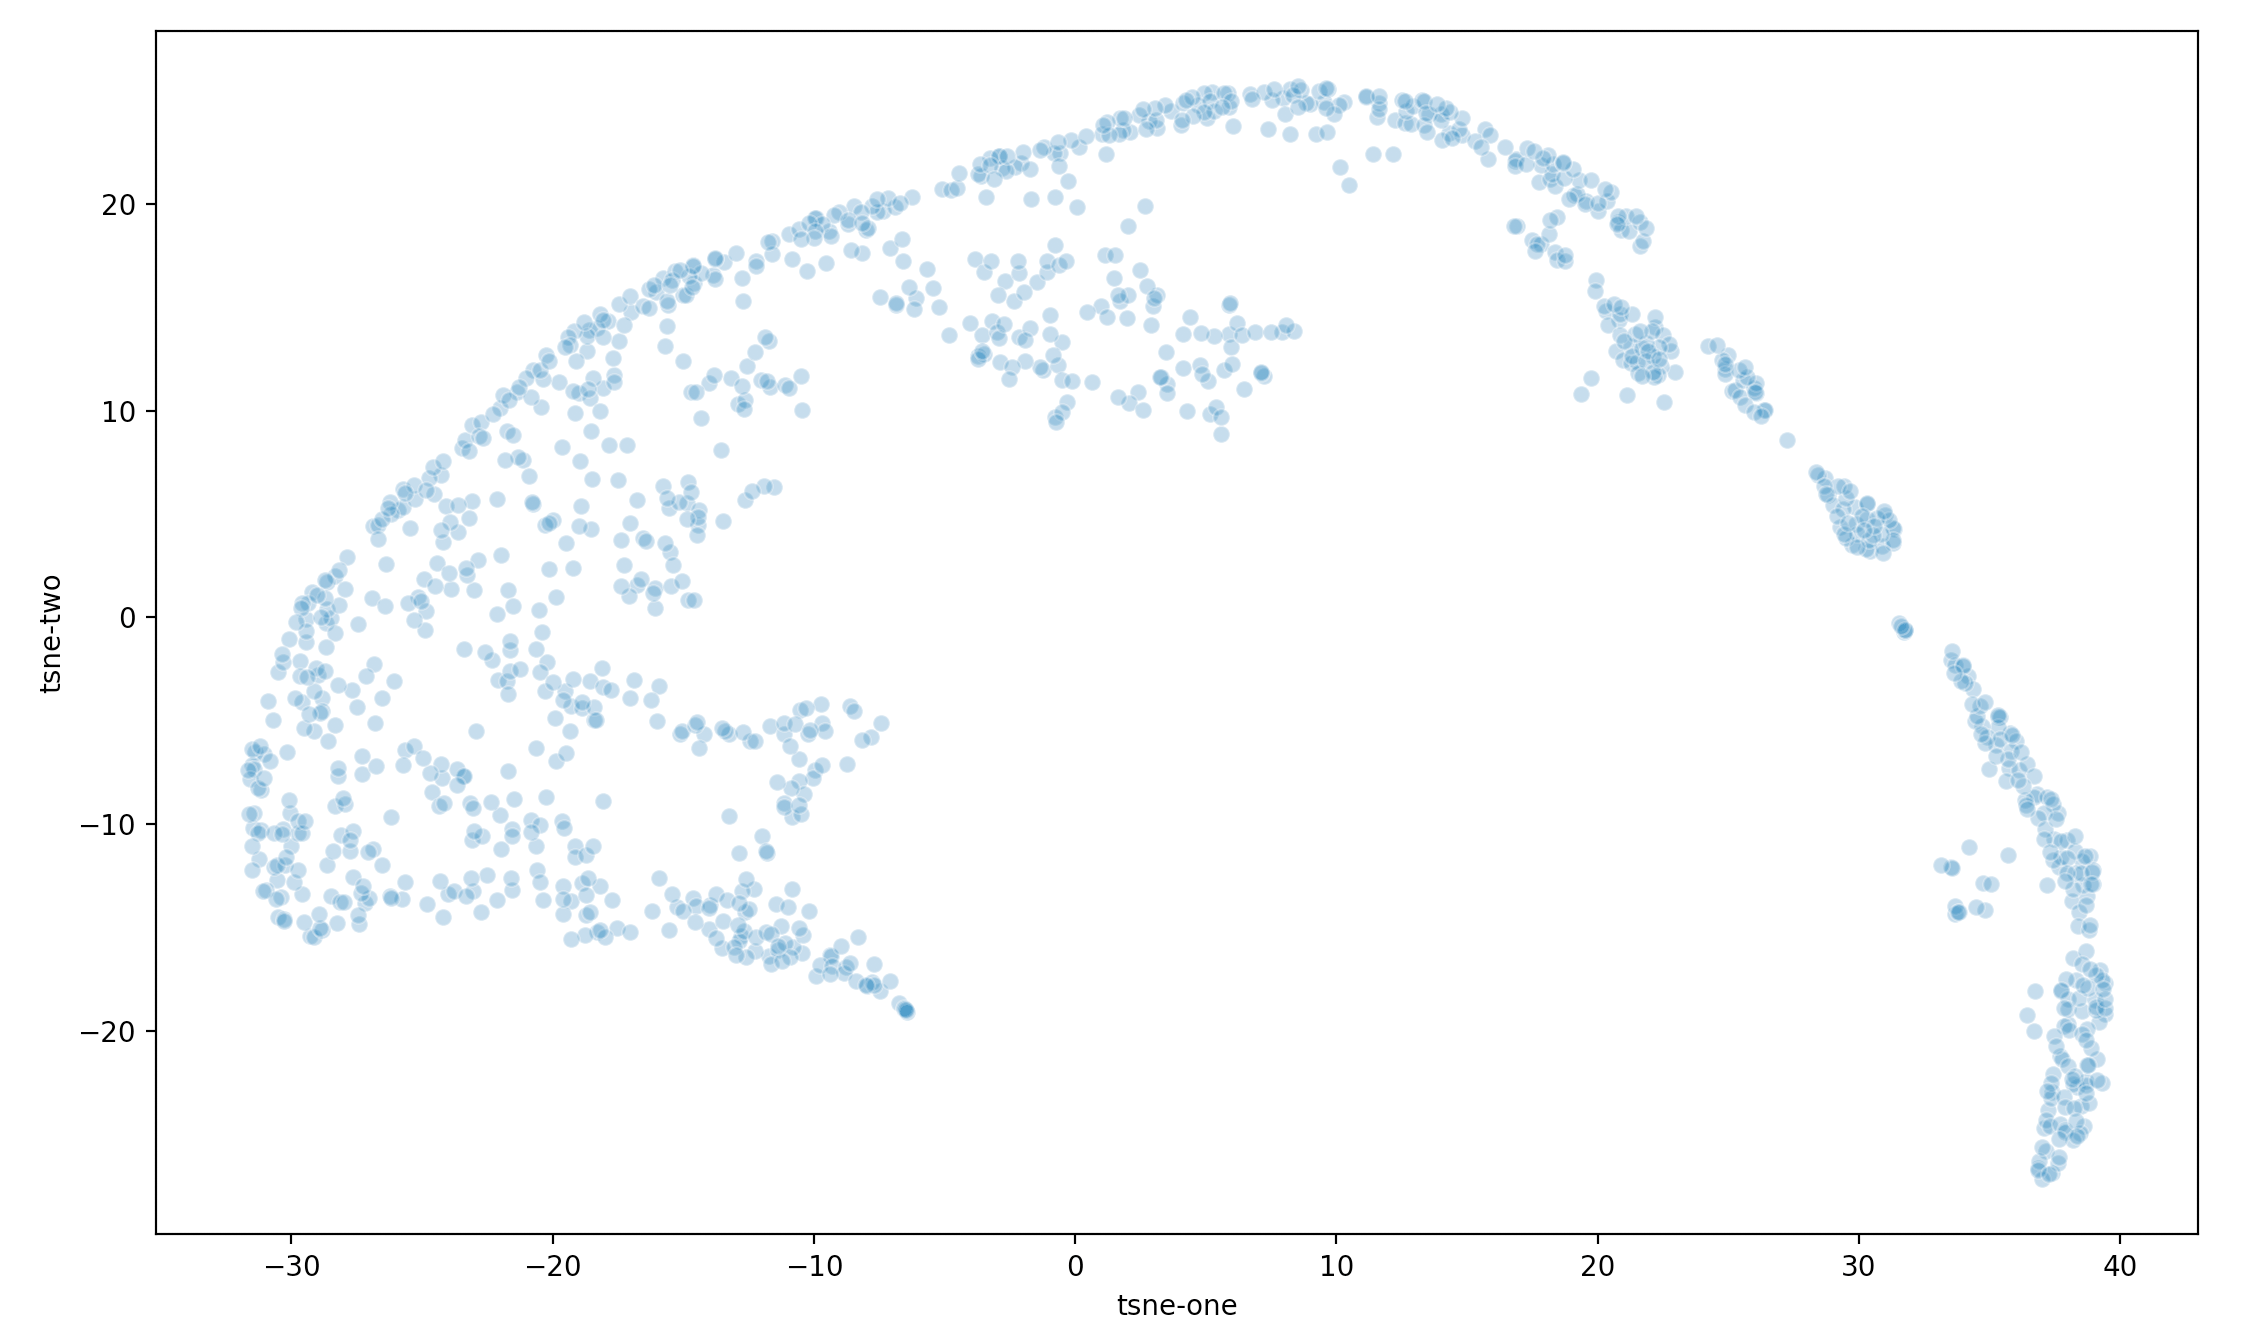
\includegraphics[width=0.5\textwidth]{./images/tsne10Files2Features.png}
  \caption{}
  \label{figure:tsne10Files2Features}
\end{figure*}

One theory was that points from a same test subject were similar and might be causing the chain. To see which data points were contained in the chain, the row index number was added as a label to each data point in the scatter plot. Furthermore, each test user data file was assigned a different random colour, so that in the plot it was visible, which data points belonged to the same user. The resulting scatter plot is visualised in figure \ref{figure:tsneTestSubjectsColor}. From this plot it can be seen, that several data points from the same test subject cluster together in the chain, indicating similarity. There are however points from each user in different locations of the chart, not only in the chain. This implied, that the chain was not being caused by the subjects. The next step was to use the data point indices and to look for similarities in the values. Several rows found in the chain were extracted from the cleaned data set, directly before being fed into the t-SNE algorithm. After comparing these, it was evident that they shared a lot of the same feature values. Rows not in the chain however had different values. Looking at the same rows in the uncleaned data set (after concatenation of the .csv data files and removal of rows with missing values), rows found in the chain had several columns all with the value 0.  Further inspection showed, that when the SCRN value was 0, LIGHT, NOTIF and the APP columns where also 0. When a smartphone screen is off, the apps are not being used, which explains why the APP columns were mostly 0. The NOTIF values were often 0, presumably because the user was not constantly receiving notifications. The environment light is also often 0 when a phone is not being used, maybe because it is in a pocket or bag. To test whether these rows were causing the chain to occur, rows with less than 50\% of values that weren't 0 were removed. As can be seen in figure \textbf{TODO: ADD FIGURE FROM LATEST}, the chain is only slightly visible.




\begin{figure*}[h]
  \centering
  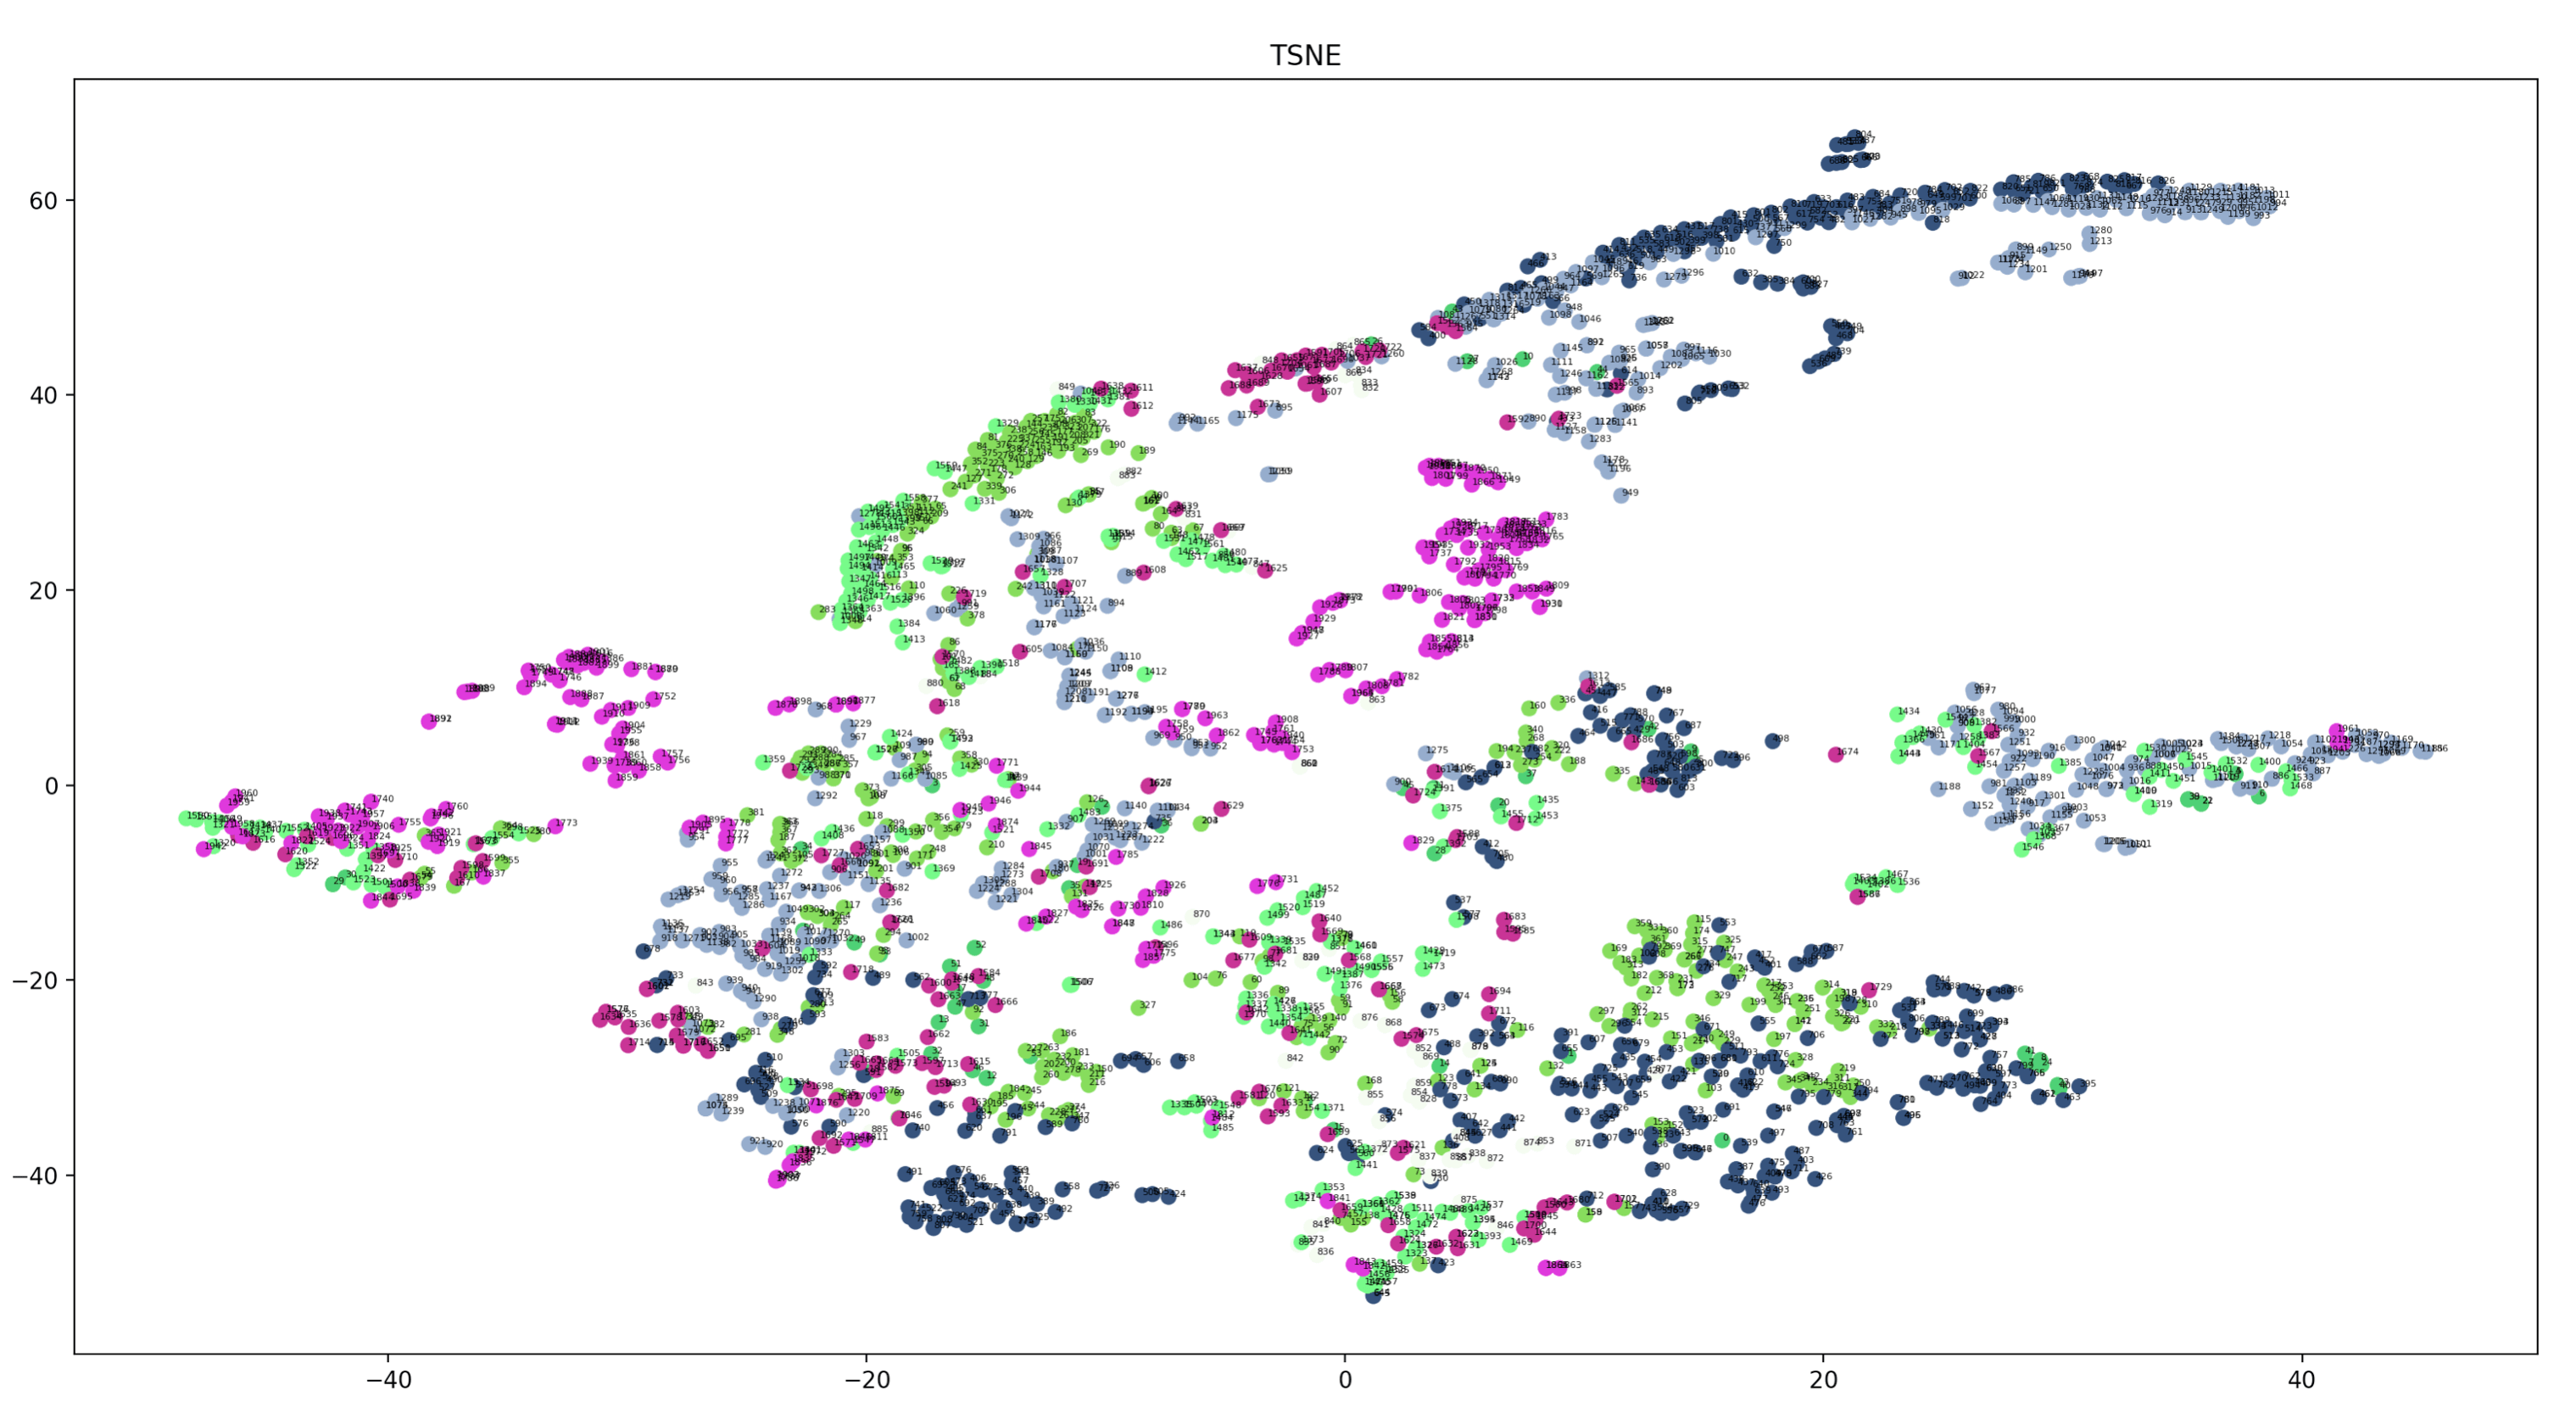
\includegraphics[width=0.9\textwidth]{./images/tsneTestSubjectsColor.png}
  \caption{}
  \label{figure:tsneTestSubjectsColor}
\end{figure*}

% \begin{figure*}[h]
%   \centering
%   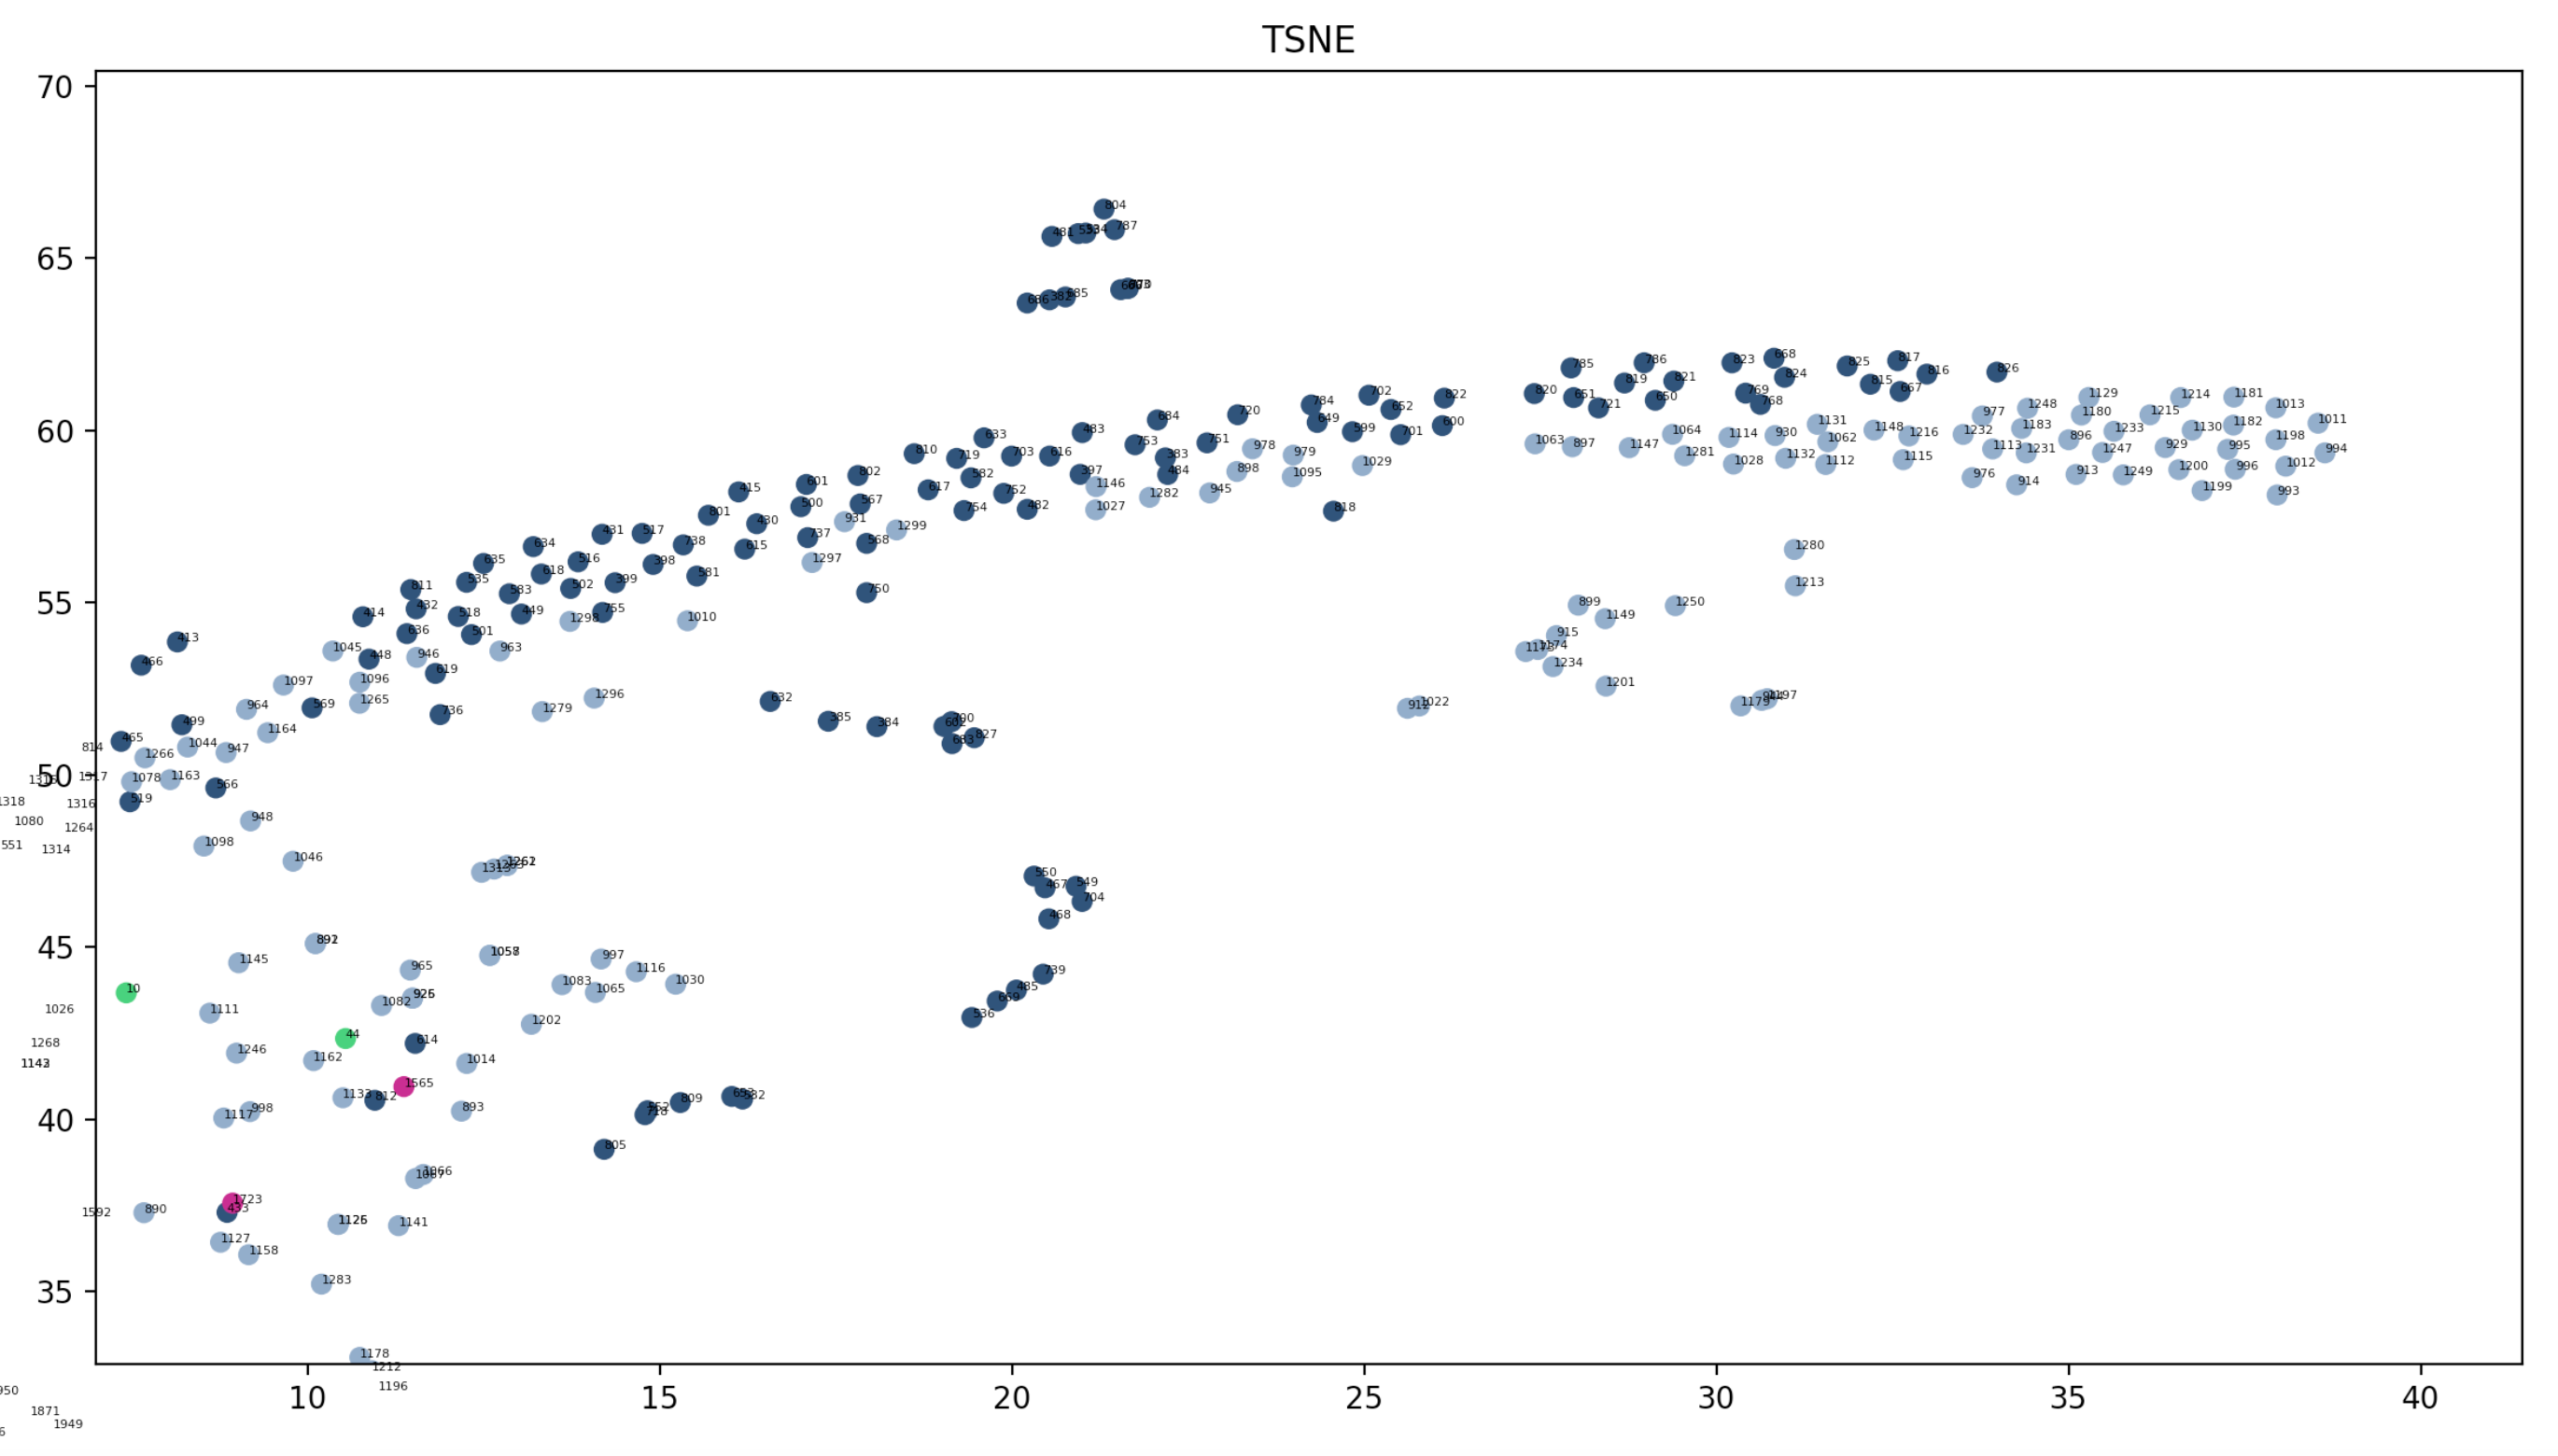
\includegraphics[width=0.9\textwidth]{./images/tsneTestSubjectsColorZoom1.png}
%   \caption{}
%   \label{figure:tsneTestSubjectsColorZoom1}
% \end{figure*}

% \begin{figure*}[h]
%   \centering
%   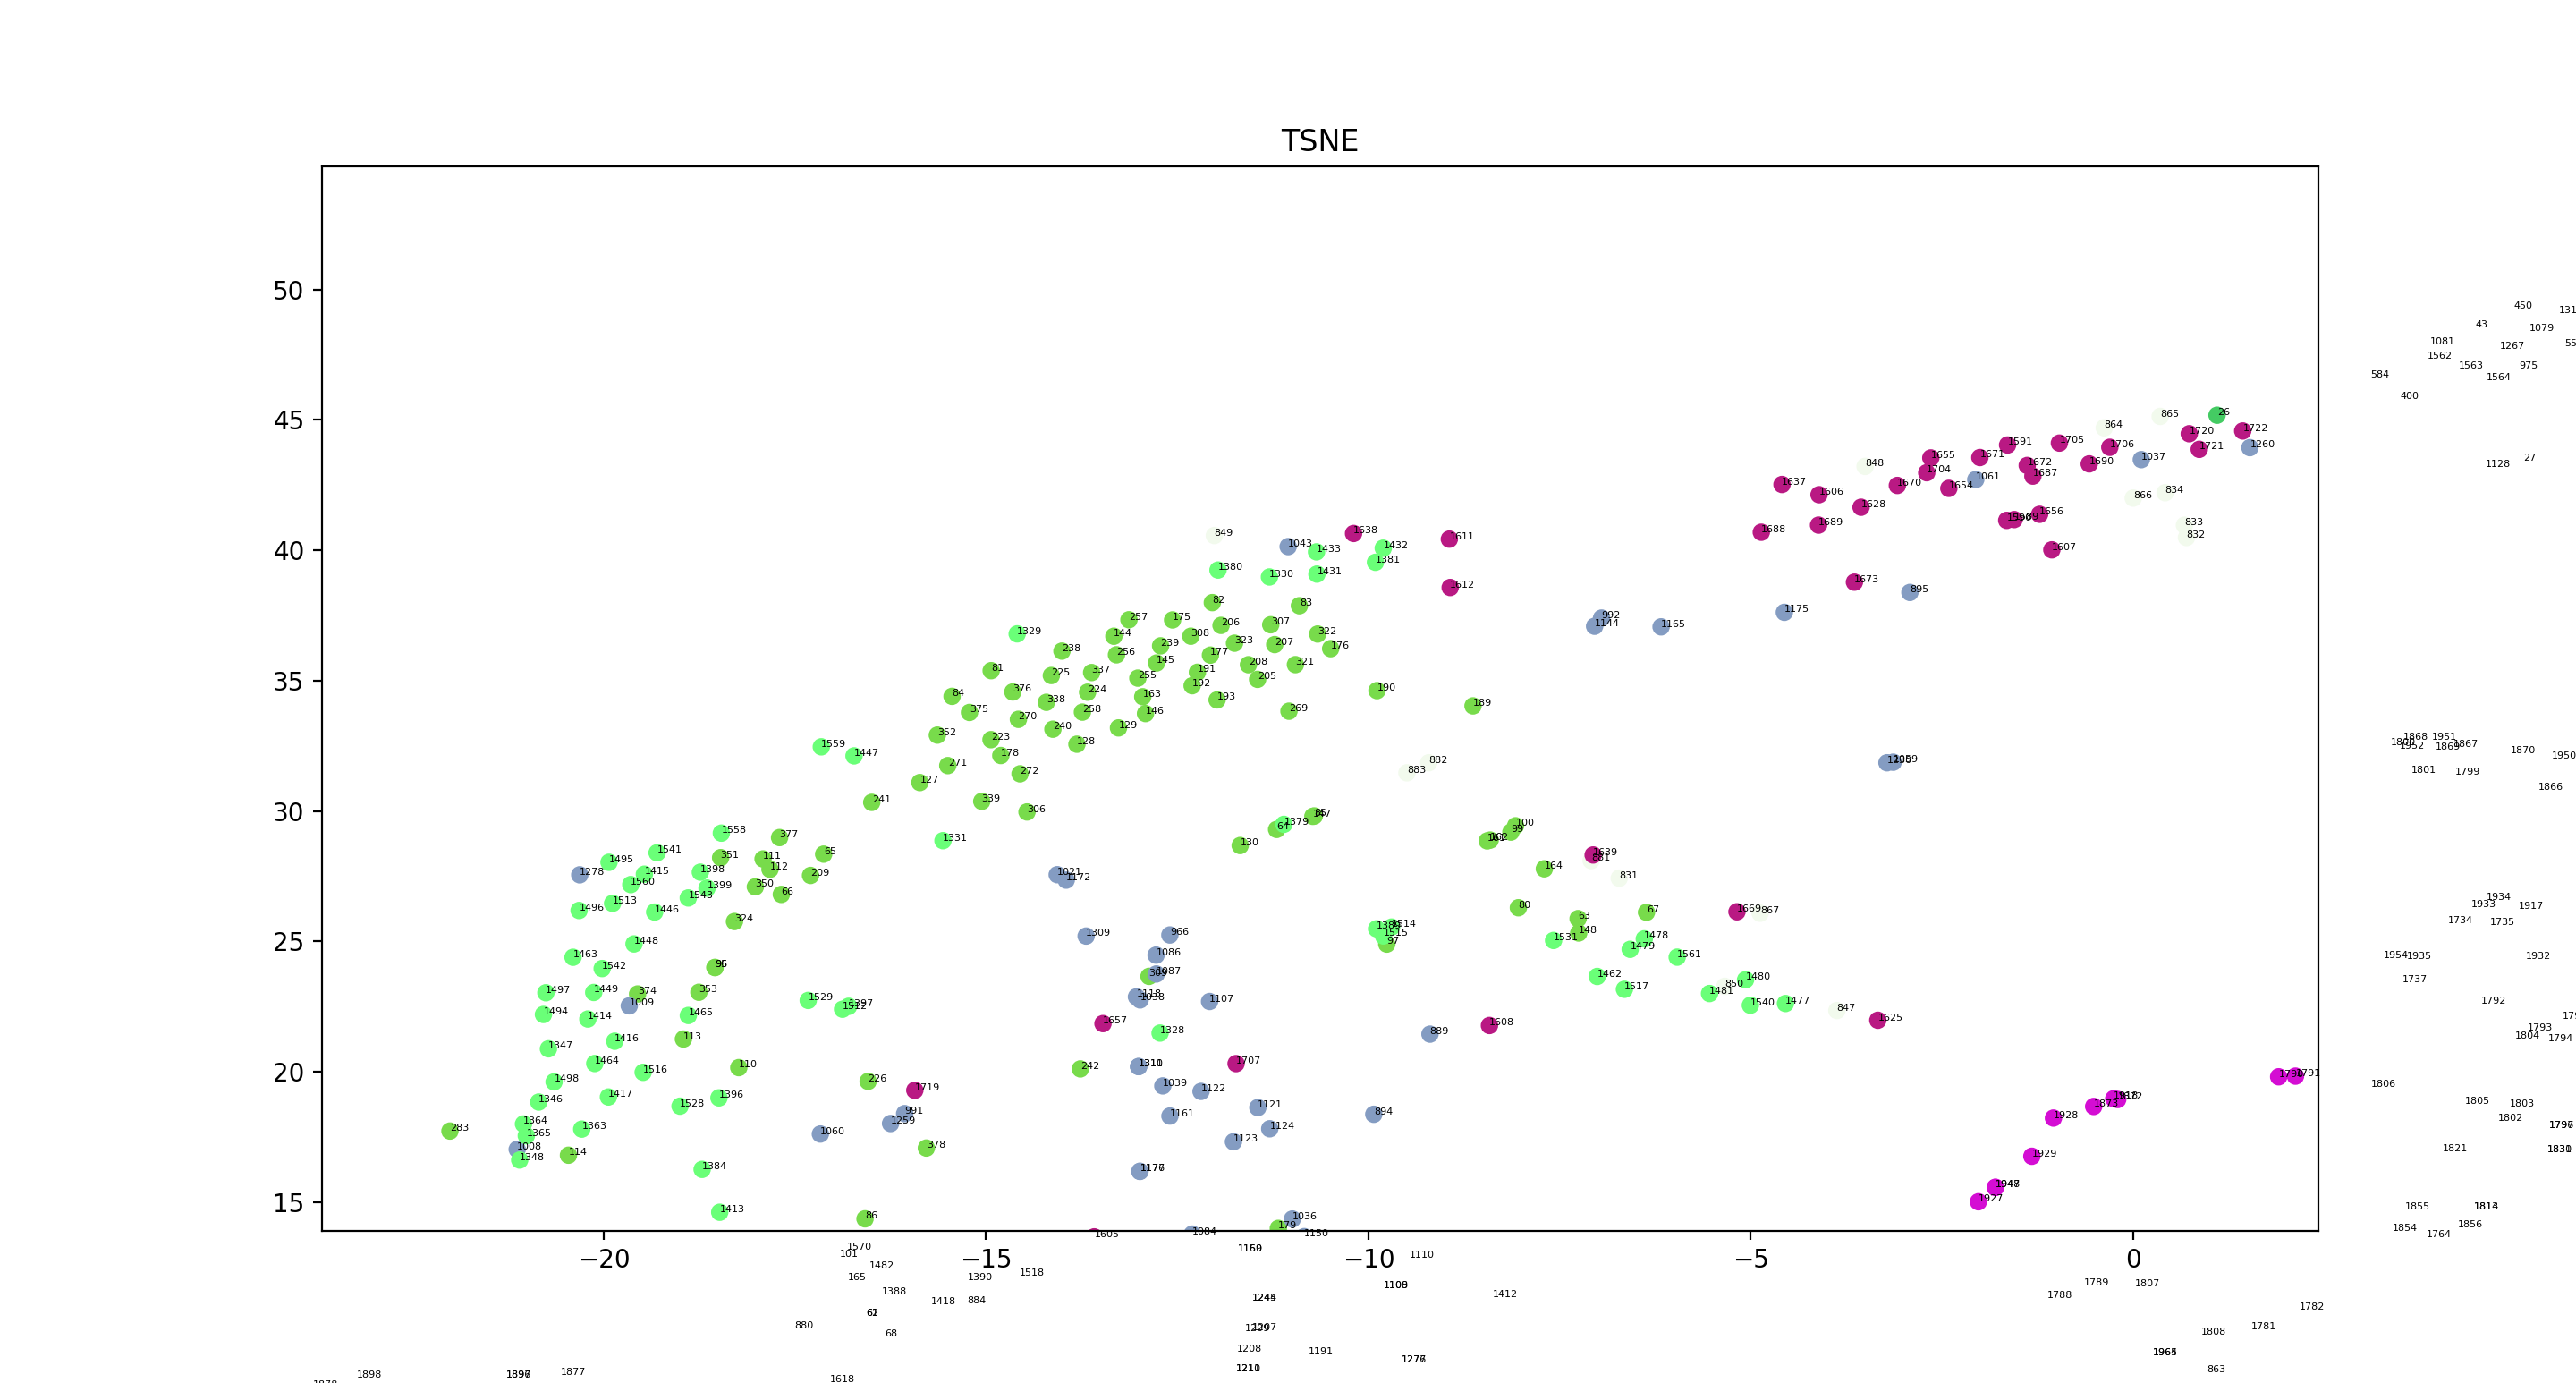
\includegraphics[width=1\textwidth]{./images/tsneTestSubjectsColorZoom2.png}
%   \caption{}
%   \label{figure:tsneTestSubjectsColorZoom2}
% \end{figure*}

% \begin{figure*}[h]
%   \centering
%   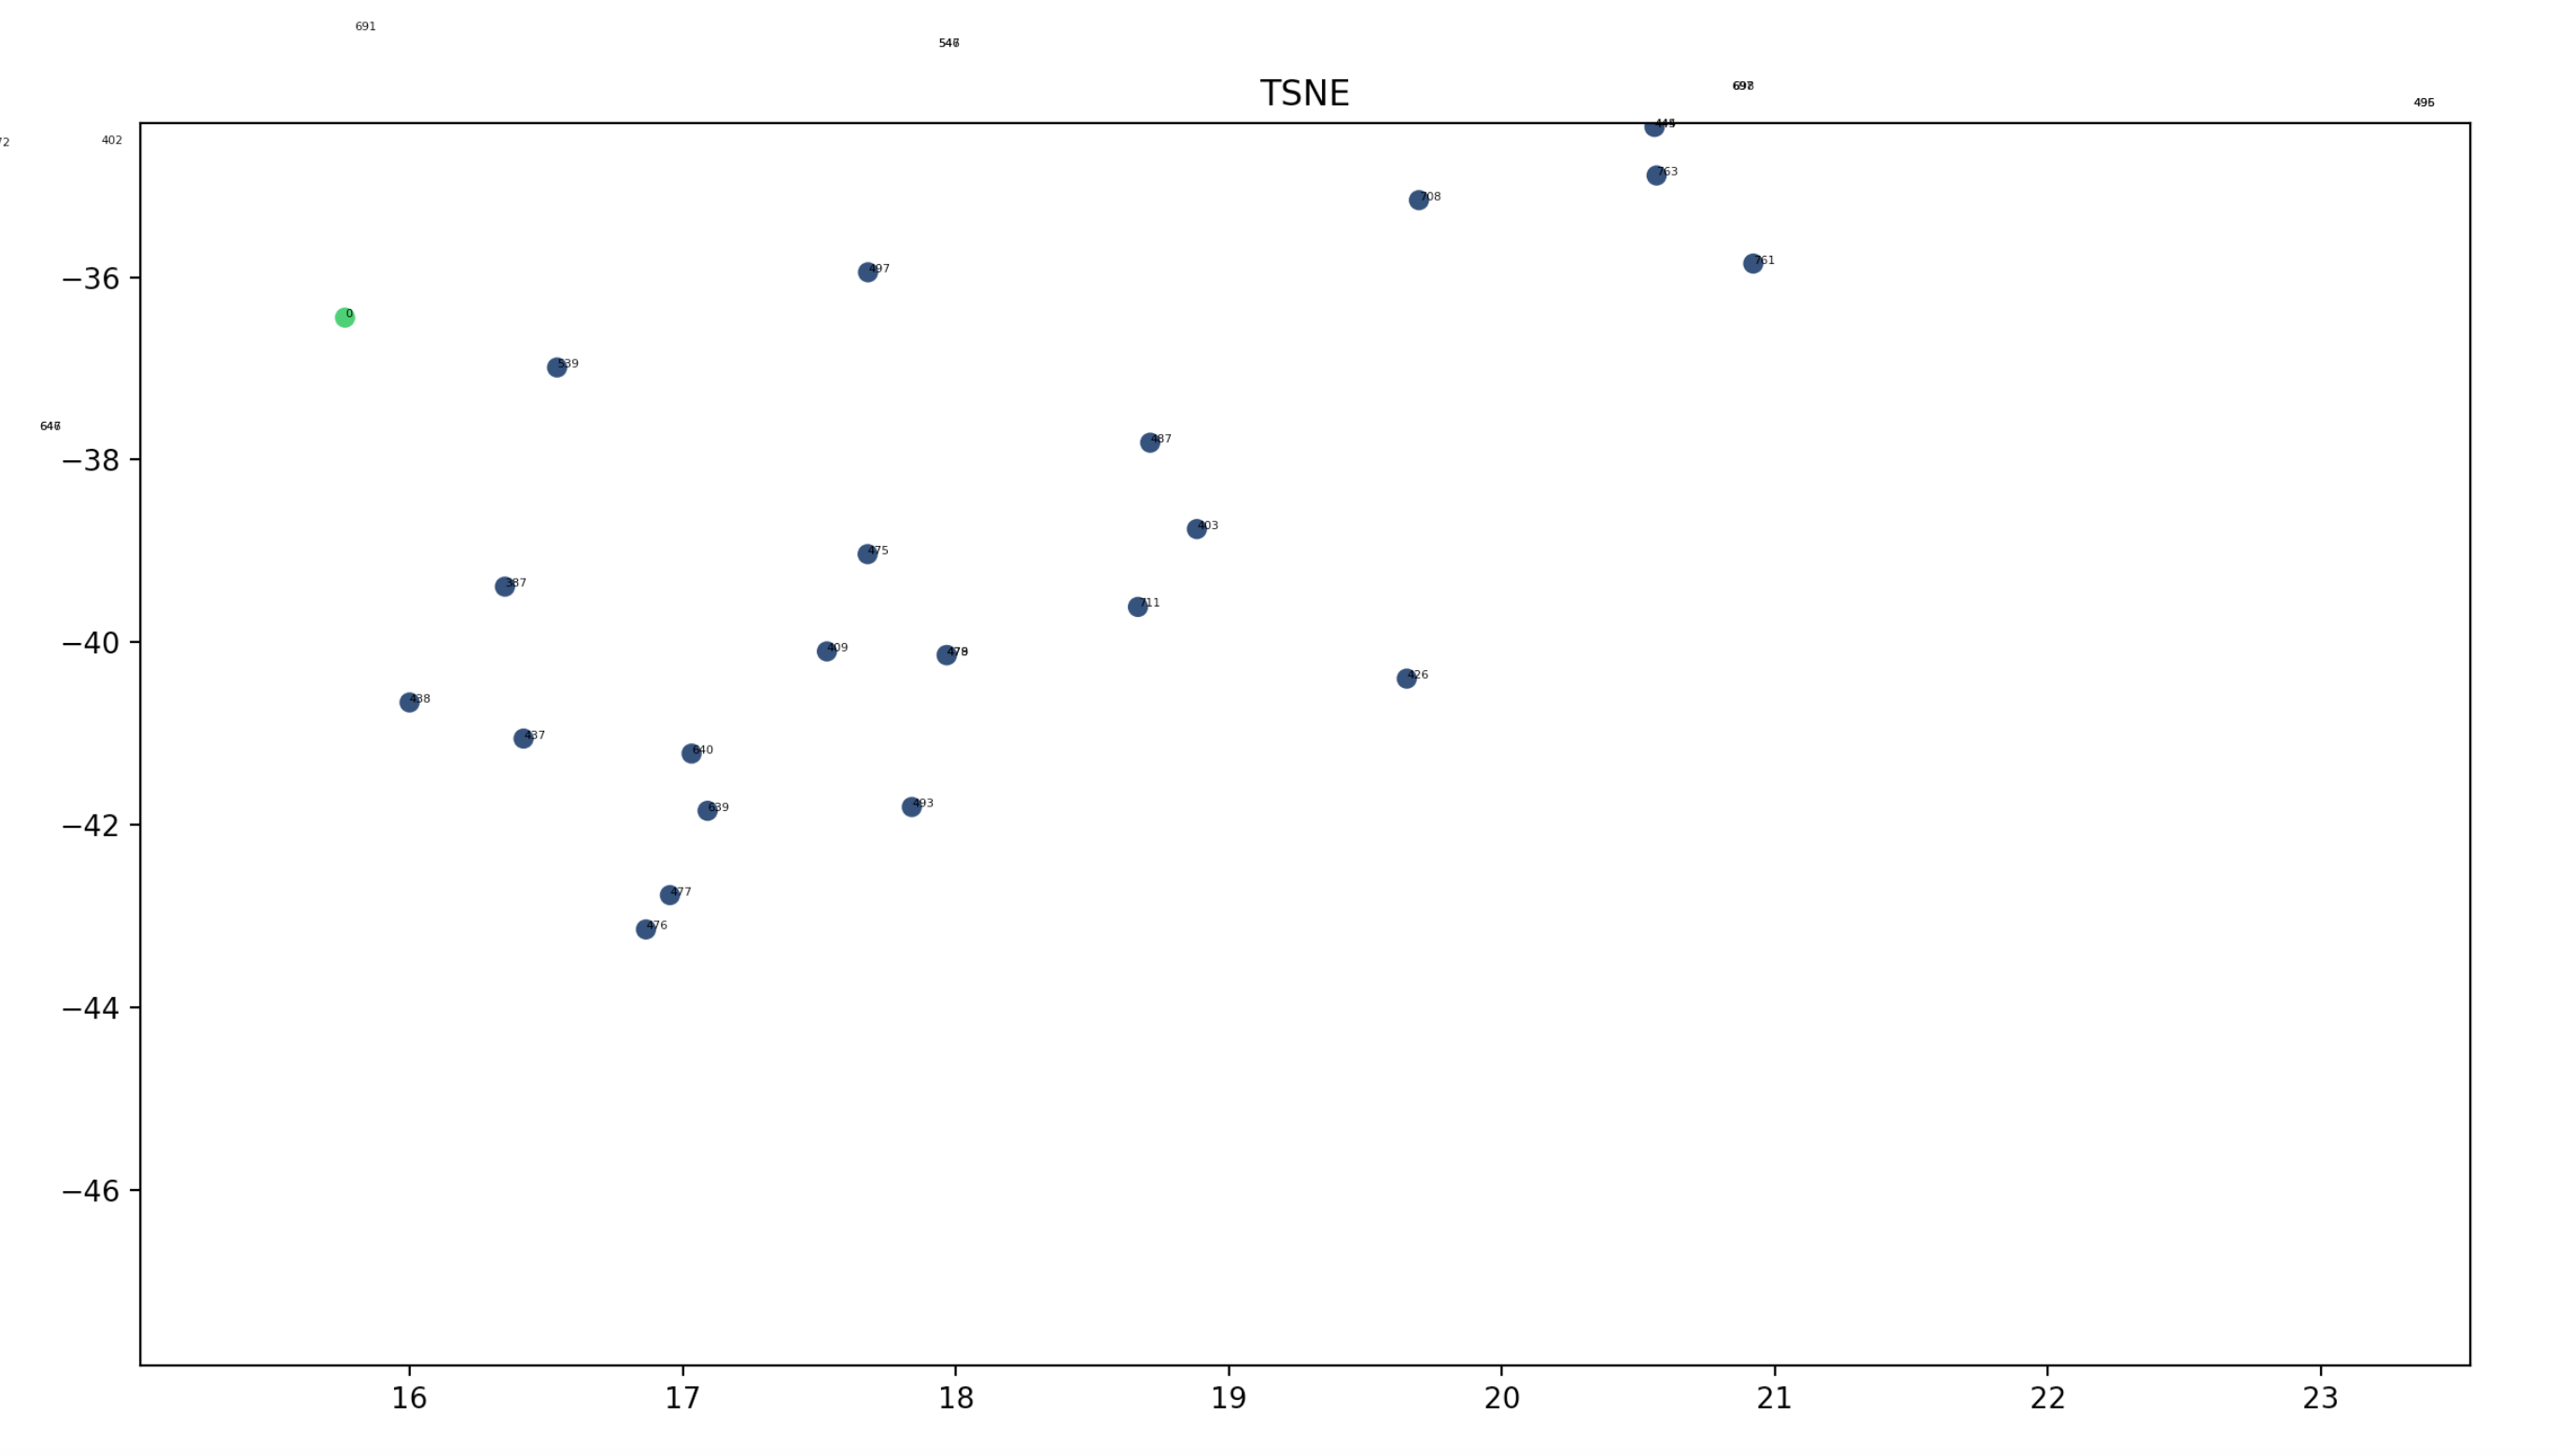
\includegraphics[width=0.9\textwidth]{./images/tsneTestSubjectsColorZoom3.png}
%   \caption{}
%   \label{figure:tsneTestSubjectsColorZoom3}
% \end{figure*}
also thought from same person



% Each unique feature only requires one column, and it therefore reduces the number of columns by 

%tod0: say with min max - high value, rest squished together
% \subsubsection{Feature reduction}
% \textbf{todo - finish or remove}
% The deletion of rows with missing values led to the loss of over 50\% of the rows in all time periods. With the intention to preserve as many of these rows as possible, columns with equal to or more than 30\% of rows with missing values were removed. This resulted in only 4 to 5 features of the original 8 being sustained. The results appeared to be unchanged and so, this feature reduction was eventually removed.


% In order to check the functionality of the data preprocessing functions, python tests were written using random mock data.


  \subsection{Dimensionality Reduction}
  \label{section:DimensionalityReduction}
  
The dimensionality reduction methods PCA and t-SNE were used to reduce the number of dimensions (number of attributes, so in this case number of columns). 

\subsubsection{PCA}
PCA was the initial approach used in the experiment. The sklearn \textit{PCA}\footnote{\url{https://scikit-learn.org/stable/modules/generated/sklearn.decomposition.PCA.html}} function was used to reduce the number of dimensions to 2, which simplified visualisation in 2D scatterplots. Before the removal of the chain (section \ref{section:chainShapedData}), the PCA allowed 65\%-95\% (depending on data preparation type and aggreation files) of the data's important structures to be accounted for in only the first two or three principle components. After the removal of the chain, the first three components only contained almost 50\% of the important structures. Of the 8 components, 7 would have been needed to account for over 90\% of these formations (for both the 1h and 3h datasets). As figure \ref{figure:PCA}a shows, the resulting data from these components did not show any significant clusters, in comparison to the t-SNE results. The principle components were further depicted in a 3D scatter plot, to evaluate whether the extra dimension revealed more structure. However, as can be seen in \ref{figure:PCA}b, only very little more structure was revealed. It is considered, that as PCA is a linear dimensionality reduction method, it might not be suitable to transform the SmartEater dataset.


\begin{figure}[H]
  \centering
  \begin{subfigure}{.475\textwidth}
    \centering
    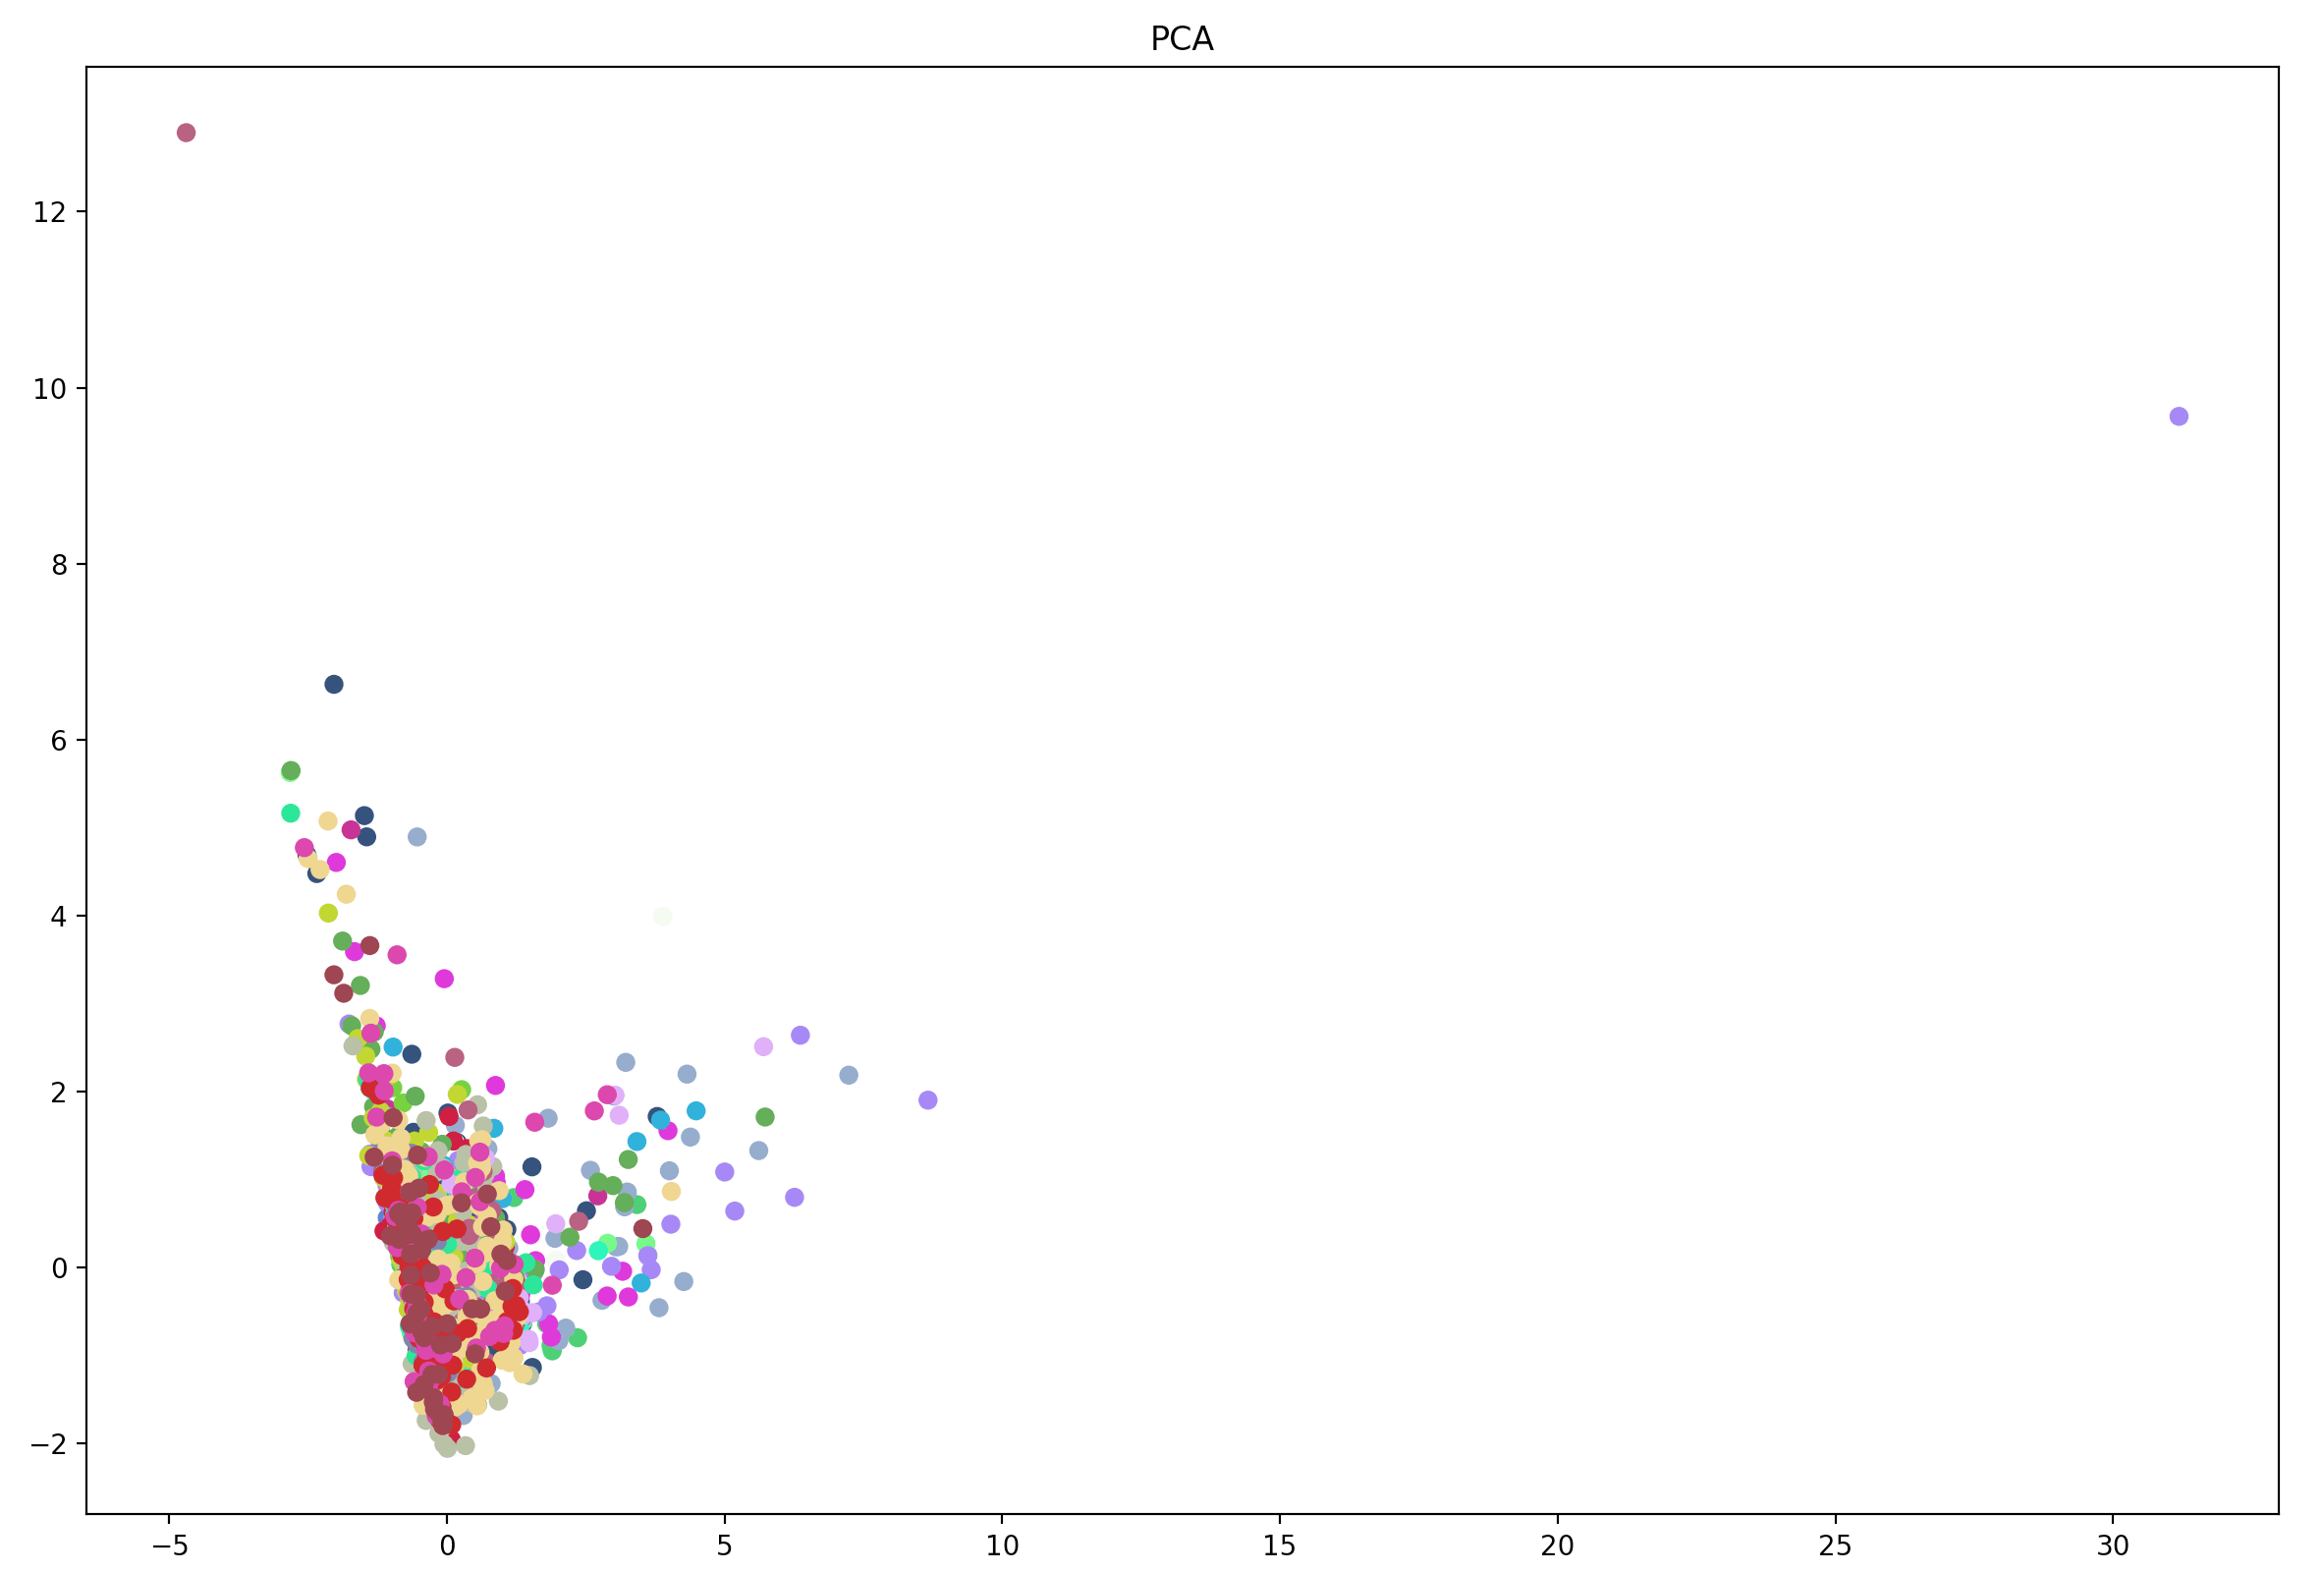
\includegraphics[width=1\textwidth]{./images/pca2d.png}
  \end{subfigure}%
  \hfill
  \begin{subfigure}{.475\textwidth}
    \centering
    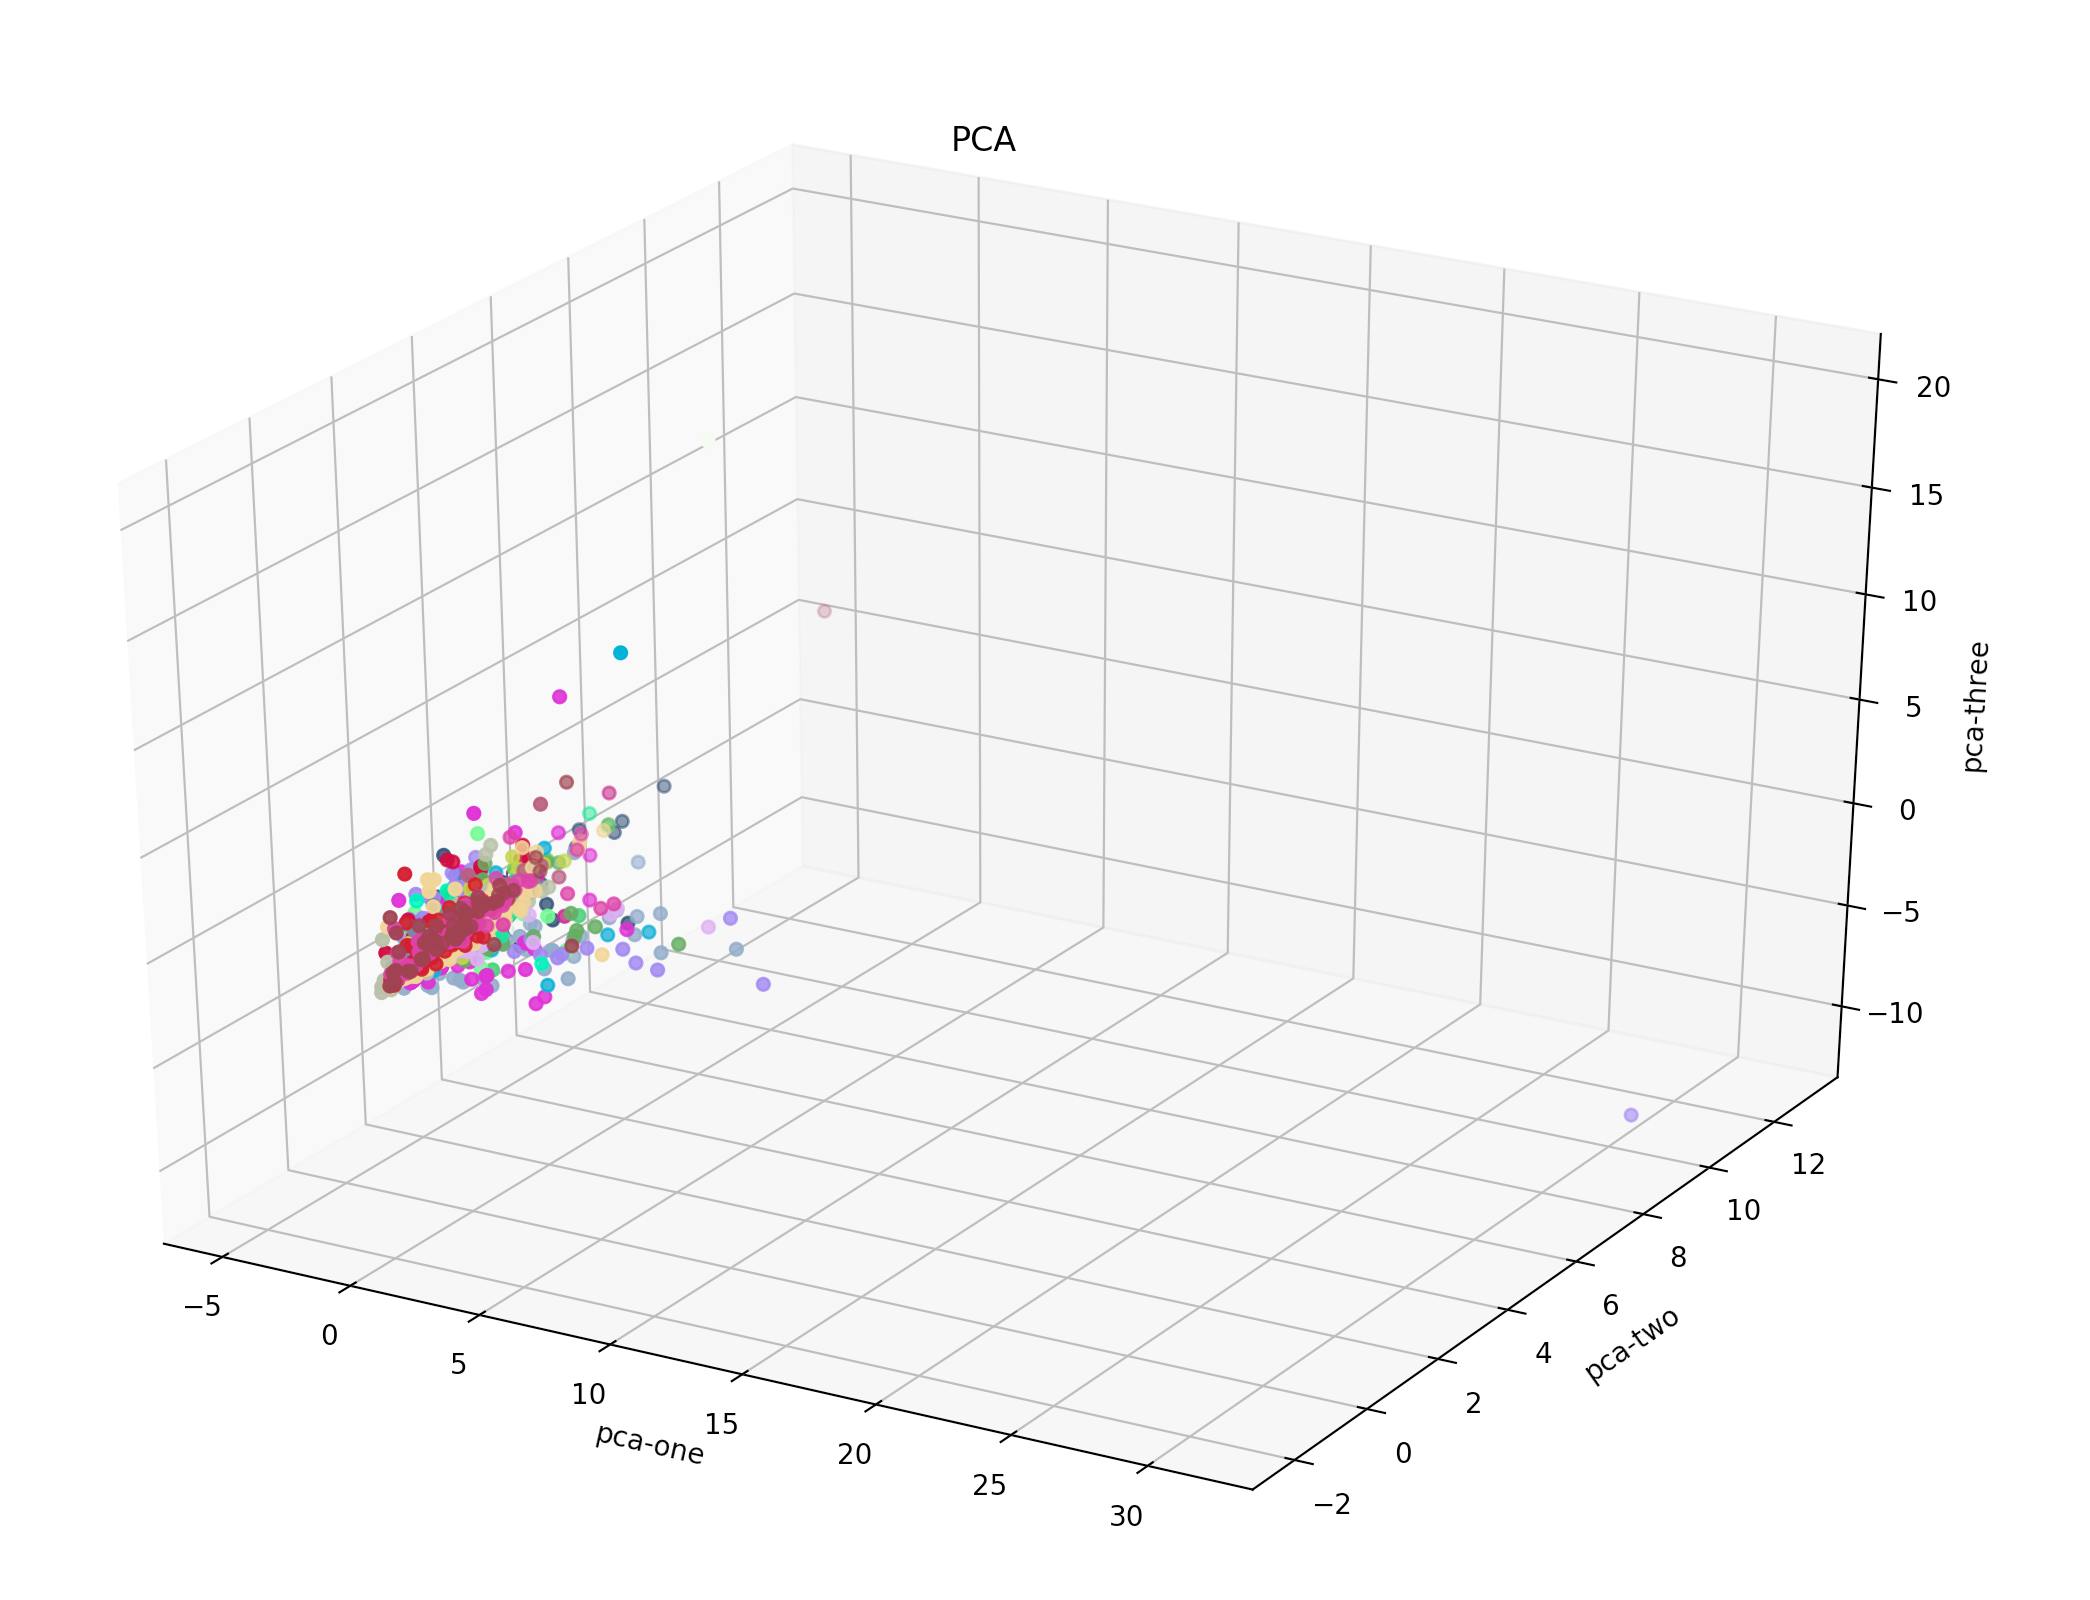
\includegraphics[width=1\textwidth]{./images/pca3d.png}
  \end{subfigure}
	\caption{2D (a) and 3D (b) scatter plots of the PCA results. The data points only appear to form one cluster with little visible structure.}
  \label{figure:PCA}
\end{figure}



\subsubsection{t-SNE}
\label{section:experimentTSNE}
The t-SNE results proved to be more significant than the PCA ones. The t-SNE algorithm was implemented using the sklearn \textit{t-SNE}\footnote{\url{https://scikit-learn.org/stable/modules/generated/sklearn.manifold.TSNE.html}} implementation.
To effectively apply the t-SNE algorithm, it was important to identify the parameters (perplexity, learning, and number of iterations) most suitable to the SmartEater dataset, as described in section \ref{section:tSNE}. The number of iterations was originally set to the default value 1000, but was later raised to 5000, to avoid receiving significantly different results each time t-SNE was run. Raising the number of iterations provided more consistent results. The overall structure of these were the same, though usually rotated differently. \textcite{wattenberg2016how} also used 5000 iterations in their experiments and stated that their t-SNE plots had reached a stable point by then.

To find suitable perplexity and learning rate t-SNE parameters to create the most distinct clusters possible, multiple 2D t-SNE scatter plots were created using different perplexity and learning rate values. 
The to determine the perplexity parameter\footnote{\textcite{wattenberg2016how} proved to be a helpful source in tuning this parameter.}, multiple values between the recommended 5 and 50, in steps of 10 (except for the first step which was 5) were tested. A perplexity of 45 was further added, since it had shown good results in tests performed before the chain described in section \ref{section:chainShapedData} was removed. The resulting scatter plots are listed in the appendix \ref{appendix:tSNEParametersPerplexity}. When visually comparing the different perplexities, the data points in the lower perplexity graphs (e.g. 5 and 10) appear to be randomly scattered and have no structure. The higher the perplexity gets, the more the data points take on structure and more distinct and well defined clusters appear. From a perplexity of 20, the 1h data files appear to start forming such clusters. When scanning the higher perplexities, it can be seen, that clusters become more separated. The scatter plots from perplexity 30 to 50 appear to have formed well defined clusters. 
%In the appendix, the plots on the left side depict the t-SNE results, while the scatter plots on the right illustrate DBSCAN clustering of these results. The DBSCAN cluster colourings were placed here to support in perceiving the differences between the t-SNE structured data and to see when the most distinct and well defined clusters were formed.

To assist in selecting the perplexity parameter, the three mathematical evaluation scores, mentioned in section \ref{section:TheoryEvaluatingClusteringResults}, were compared. Figure \ref{figure:perplexityEvaluationScores} displays the Silhouette Coefficient, Davies-Bouldin Index, and Caliński-Harabasz Index, calculated for the DBSCAN and OPTICS clusterings from different perplexities. As explained in section \ref{section:TheoryEvaluatingClusteringResults}, the Silhouette Score indicates better, denser clustering, when it is closer to 1, and incorrect clustering if the value is close to -1. The lower of two Davies-Bouldin Index and the higher of the Caliński-Harabasz Index scores suggests better clustering. The green highlighted values illustrate the best values (best defined and distinct clusters in that score for that clustering method, for the mentioned dataset) for the one hour or three hour time lengths, whilst the darker green fields also feature the overall best value (1h and 3h files). 
The number of these best scoring fields will henceforth be referred to as number of "wins". With 4 wins, a perplexity of 20 has the highest number of best achieving score values. The perplexities of 10, 40, and 45 tied in second place with 2 wins. While according to the scores, perplexity 20 creates the best clusters, visually the clusters appear better defined with a perplexity between 30 and 50. For this reason, the focus of the comparison of the scores was moved to the scores that were highest, whose perplexity was between 30 and 50. Perplexity 40 had the most wins in figure \ref{figure:perplexityEvaluationScoresDetailed} and was chosen as the final parameter. These tests were conducted a second time (see appendix \ref{appendix:compareAveragePerplexity}), using the average of two different t-SNE results for each of the datasets. While the scores are slightly different, a perplexity of 40 was again the overall best achieving value.

\begin{figure}
  \centering
  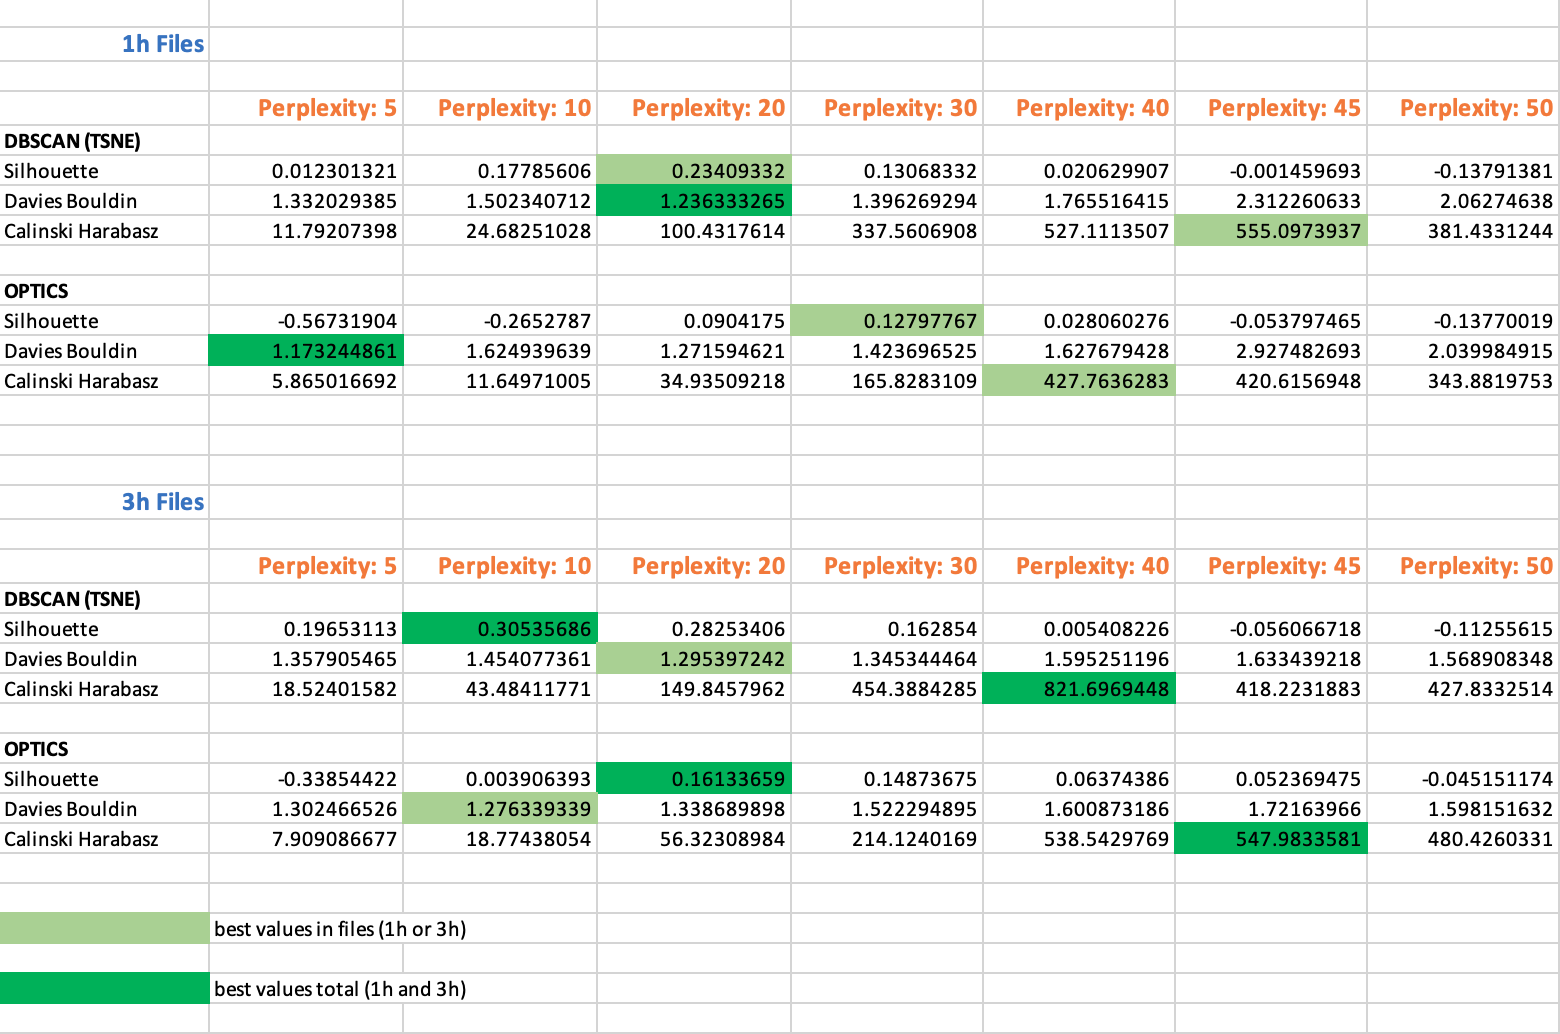
\includegraphics[width=0.8\textwidth]{./images/tsneParametersTest/perplexity/perplexityEvaluationScores.png}
  \caption{Comparison of Silhouette Coefficient, Davies-Bouldin Index, and Caliński-Harabasz Index for different t-SNE \textbf{perplexities} in steps of 5 and 10. The lighter green highlighted values indicate the best values of that file aggregation (1h or 3h files). The dark green highlighted values illustrate the overall best values over all files (1h and 3h files).}
  \label{figure:perplexityEvaluationScores}
\end{figure}

\begin{figure}
  \centering
  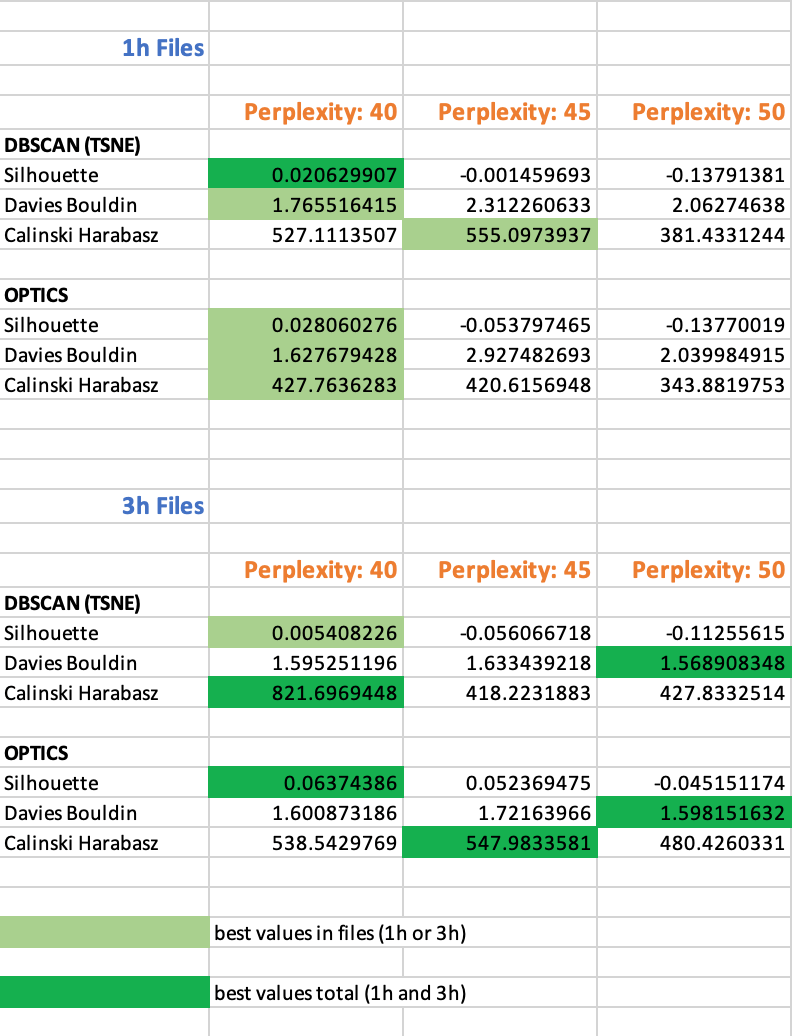
\includegraphics[width=0.4\textwidth]{./images/tsneParametersTest/perplexity/perplexityEvaluationScoresDetailed.png}
  \caption{Comparison of the evaluation scores of the top three perplexity candidates 40, 45, and 50. The lighter green highlighted values indicate the best values of that file aggregation (1h or 3h files). The dark green highlighted values illustrate the overall best values over all files (1h and 3h files).}
  \label{figure:perplexityEvaluationScoresDetailed}
\end{figure}


The same principle was used to determine the ideal value for the learning rate parameter. The sklearn t-SNE documentation states, that the learning rate is normally set between 10 and 1000, hence the learning rate in the scatter plots was chosen in this interval.
The various resulting scatter plots can be seen in the appendix \ref{appendix:tSNEParametersLearningRate}. The differences in the arrangement of the data points over the plots is not as substantial as it was when testing for the perplexity. The results, listed in figure \ref{figure:learningRateEvaluationScores} revealed, that the learning rate 10 scores highest with a learning rate of 800 coming in second. Since roughly 200 steps were taken between the learning rate values, smaller steps were taken (i.e. 50) around the winning value, to see if an even better performance could be accomplished (figure \ref{figure:learningRateEvaluationScoresDetailed}, in appendix \ref{appendix:comparelearningRateDetailed}). While 10 still achieved best in the one hour time length files, 800 came top in the three hour files, indicating that 10 might not be the best rate for these. Consequently, the values 20 and 30 were also evaluated (figure \ref{figure:learningRateEvaluationScoresDetailed2}, in appendix \ref{appendix:comparelearningRateDetailed}). While a learning rate of 10 still came top in the one hour files, 30 came top in the three hour files. With the hope of finding a value in between 10 and 30 that satisfied both time lengths, the learning rates 10, 15, 20, 25, and 30 were ultimately compared exclusively. The results in figure \ref{figure:learningRateEvaluationScoresDetailed3} exposed, that this final comparison lead to the learning rate 20 being the most suitable. 

As with the perplexity, the learning rate tests were also reproduced, averaging two different t-SNE outcomes. The results are illustrated in appendix \ref{appendix:compareAverageLearningRate}. 800 appears to be more dominant than the lower parameter values (e.g. 10 and the favourite 20). To further compare 20 and 800, appendix \ref{appendig:compareLearningRate20and800} contains a table (figure \ref{figure:learningRateEvaluationScoresAverageDetailed4}) comparing 4 different runs of scores from average t-SNE results. With 2 wins more than 20, 800 has the overall better score results. Figures \ref{figure:1h-learningRateComparison20and800} and \ref{figure:3h-learningRateComparison20and800} visually compare the scatter plots created with a learning rate of 20 and 800. The plots and clusters appear very similar. The clusters from perplexity 20 however seem slightly more compact (less smaller clusters). A learning rate of 20 was thus selected for the final learning rate parameter. However, 800 was also used in the final results.


The final t-SNE parameters, from which the results were then used by the DBSCAN and OPTICS clustering methods in the next section, were as follows: perplexity = 40, learning\_rate = 20, and n\_iter = 5000. A run of the resulting graphs are depicted in figures \ref{figure:finalTSNE1h} and \ref{figure:finalTSNE3h}.


\begin{figure}
  \centering
  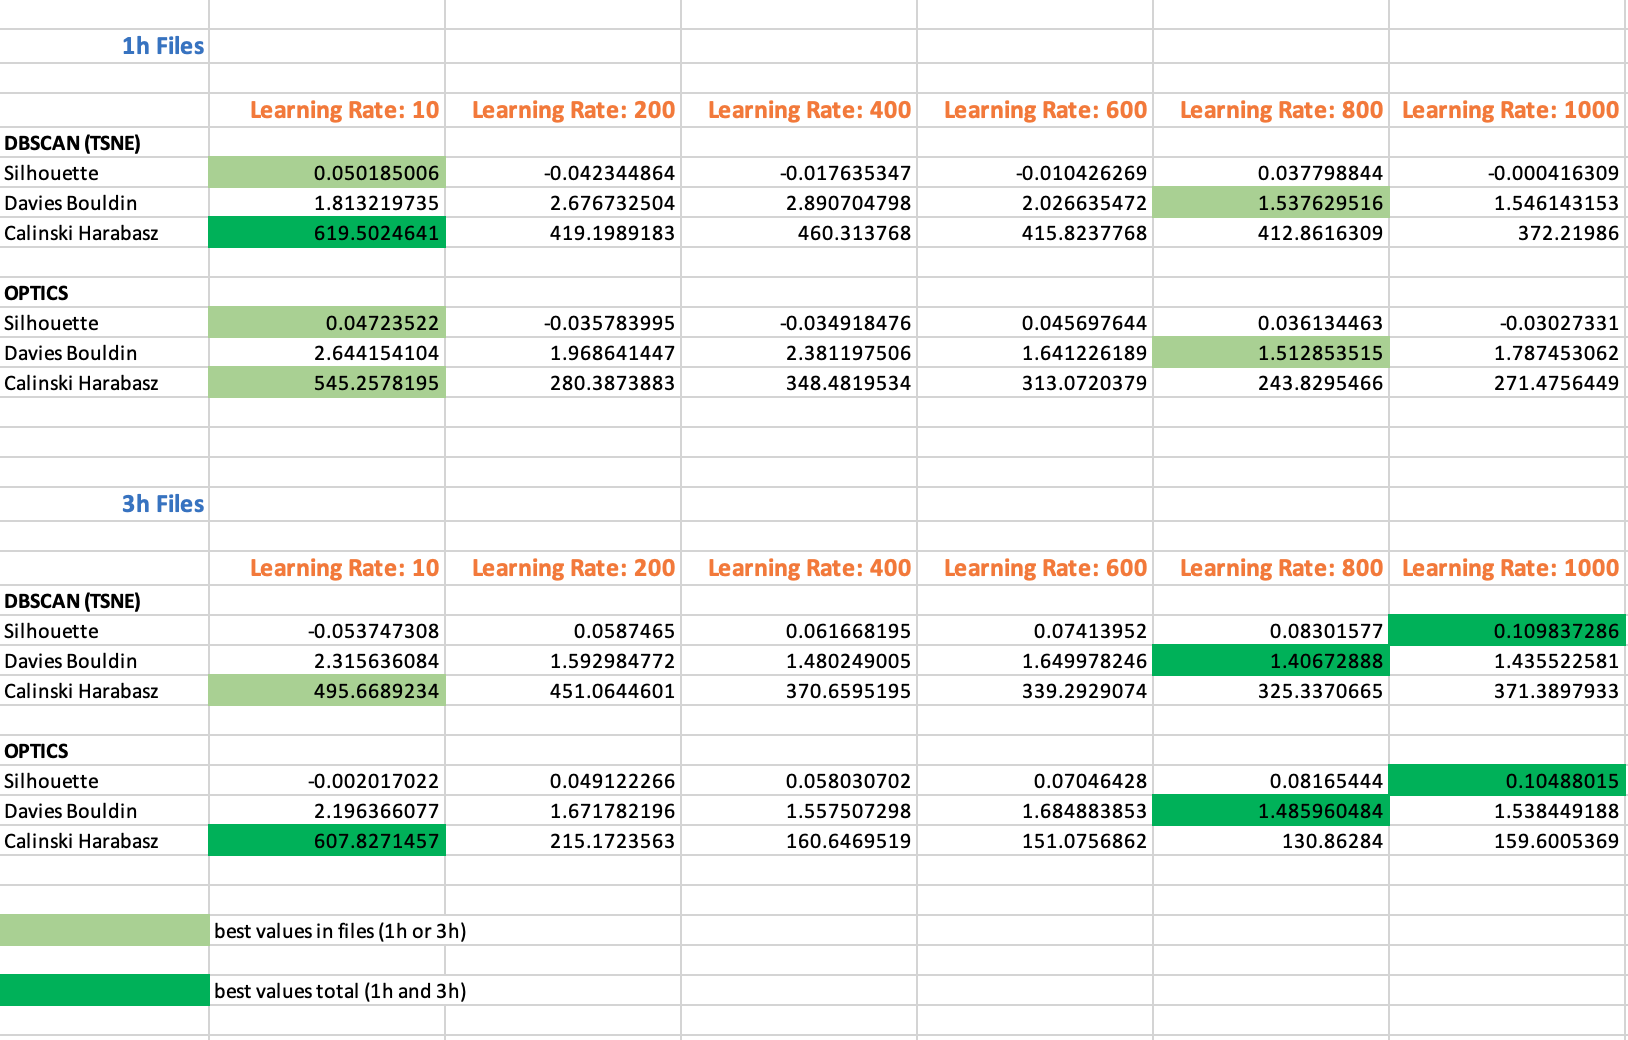
\includegraphics[width=0.8\textwidth]{./images/tsneParametersTest/learningRate/learningRateEvaluationScores.png}
  \caption{Comparison of Silhouette Coefficient, Davies-Bouldin Index, and Caliński-Harabasz Index for different t-SNE \textbf{learning rate} values, in  (except the first step of 190). The lighter green highlighted values indicate the best values of that file aggregation (1h or 3h files). The dark green highlighted values illustrate the overall best values over all files (1h and 3h files).}
  \label{figure:learningRateEvaluationScores}
\end{figure}


\begin{figure}
  \centering
  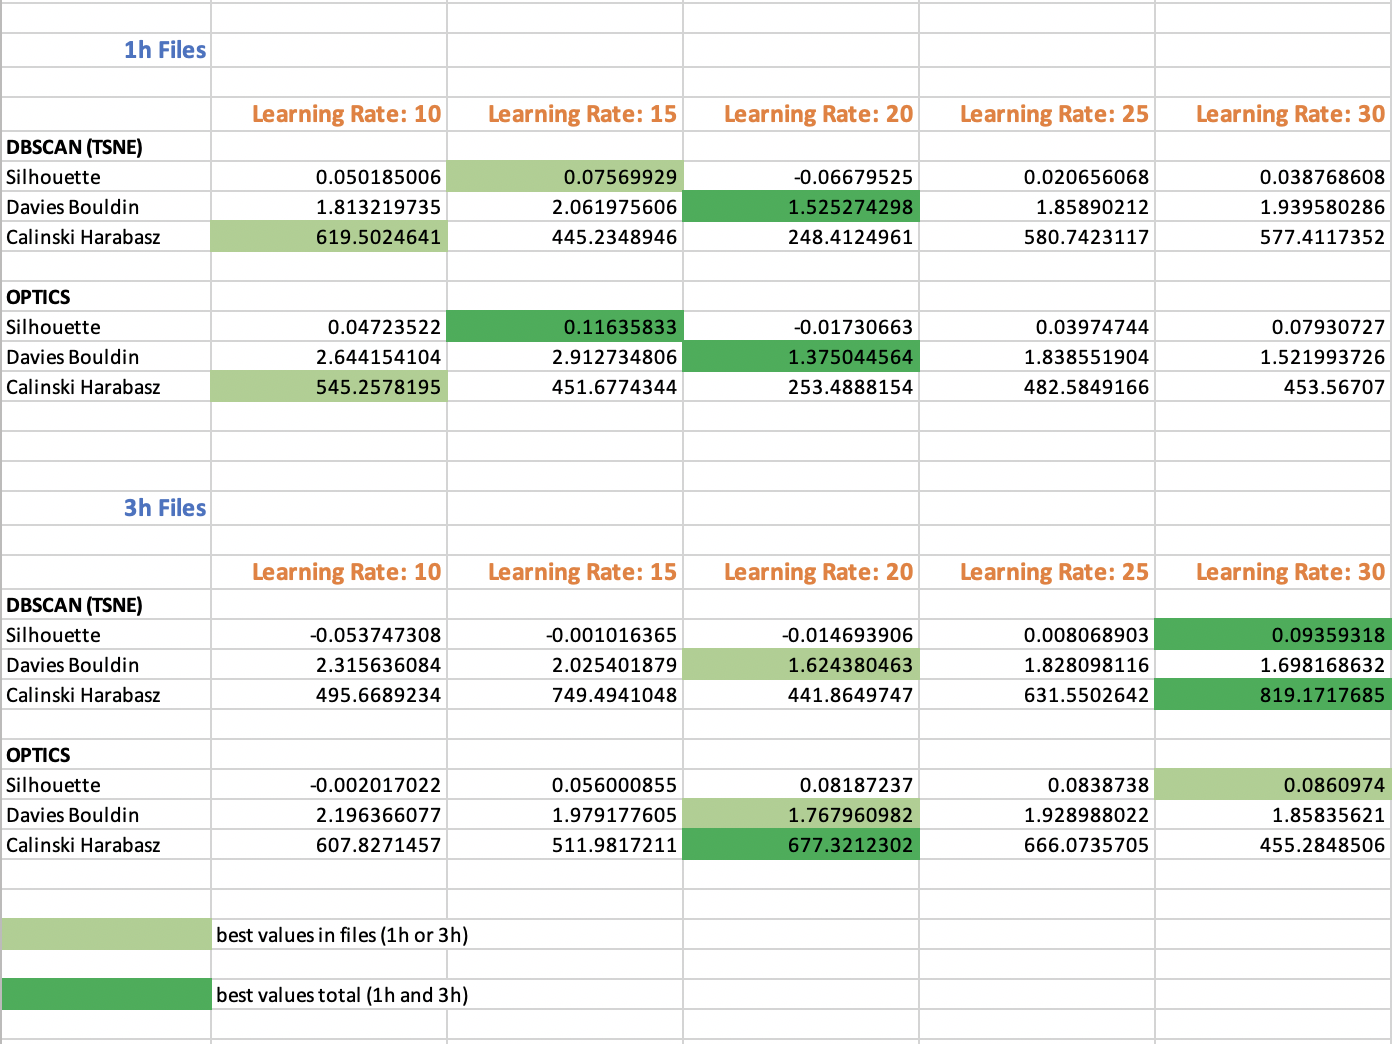
\includegraphics[width=0.8\textwidth]{./images/tsneParametersTest/learningRate/learningRateEvaluationScoresDetailed3.png}
  \caption{Comparison of Silhouette Coefficient, Davies-Bouldin Index, and Caliński-Harabasz Index for different t-SNE \textbf{learning rate} values. The goal is to find a learning rate value between 10
  and 30, that satisfies both the 1h and 3h datasets. The lighter green highlighted values indicate the best values of that file aggregation (1h or 3h files). The dark green highlighted values illustrate the overall best values over all files (1h and 3h files).}
  \label{figure:learningRateEvaluationScoresDetailed3}
\end{figure}



\begin{figure}
  \centering
	\begin{subfigure}{.5\textwidth}
    \centering
    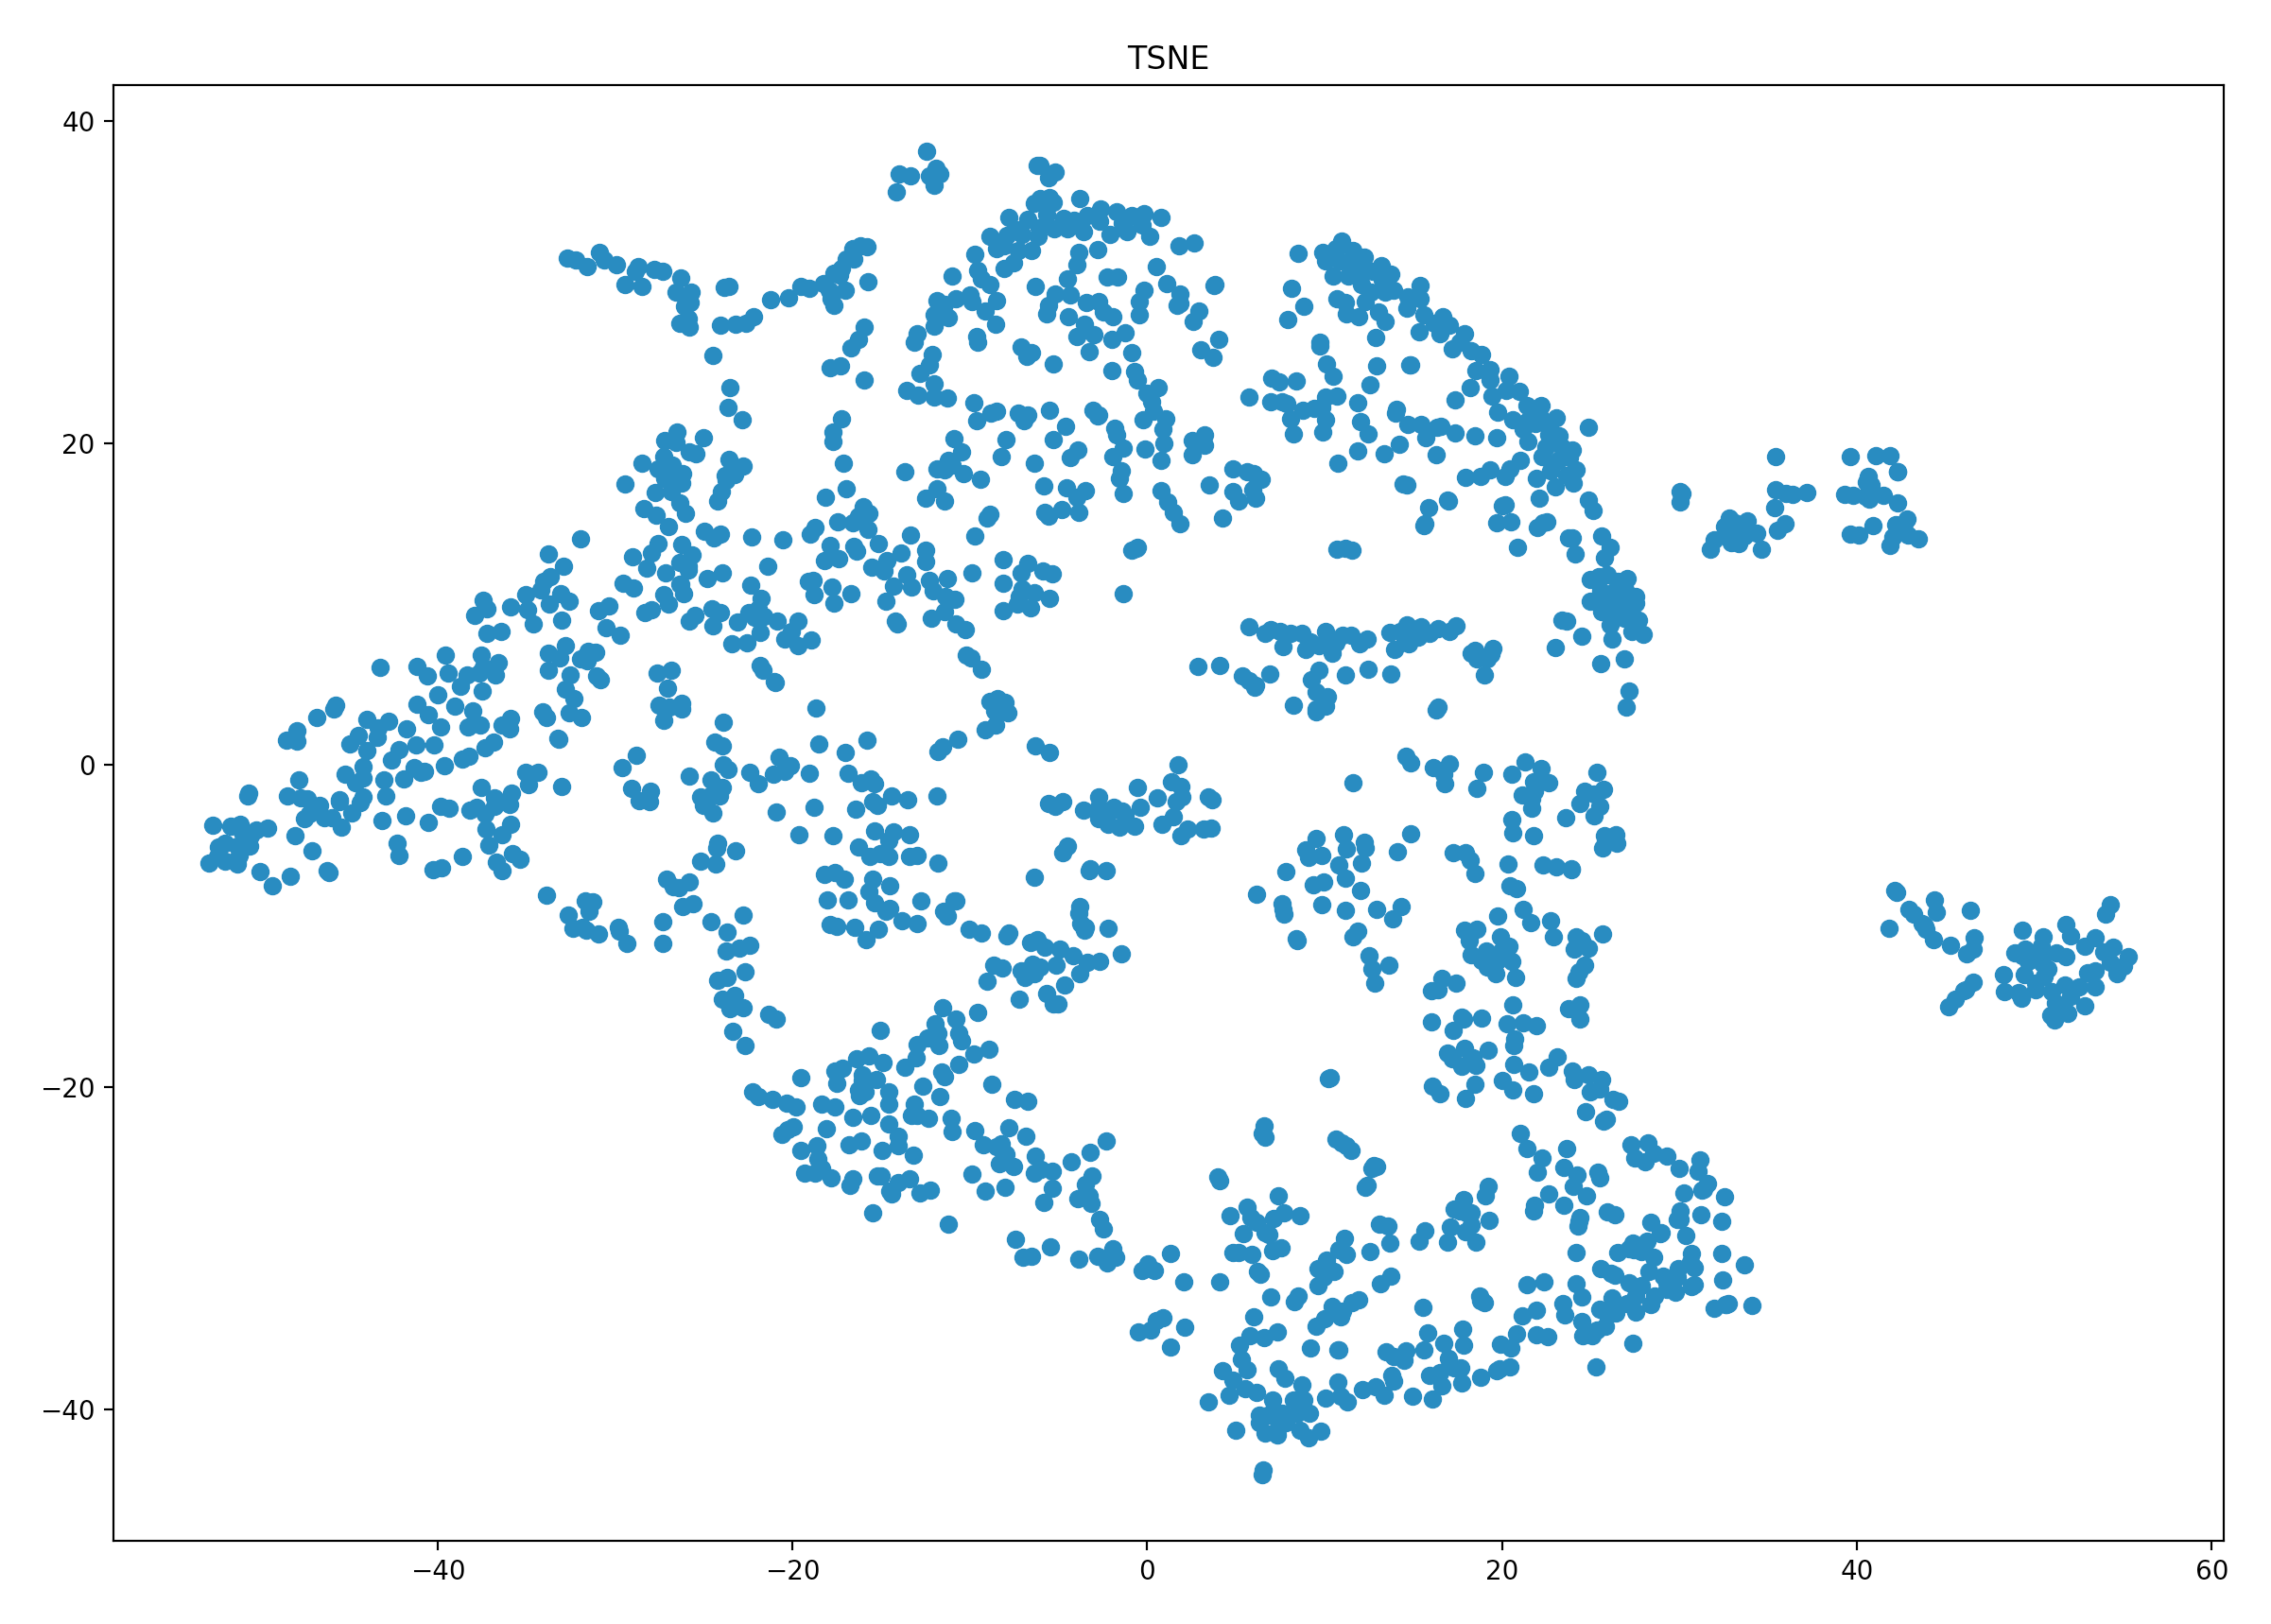
\includegraphics[width=0.9\textwidth]{./images/tsneParametersTest/1h-1-finalTSNE.png}
  \end{subfigure}%
  \begin{subfigure}{.5\textwidth}
    \centering
    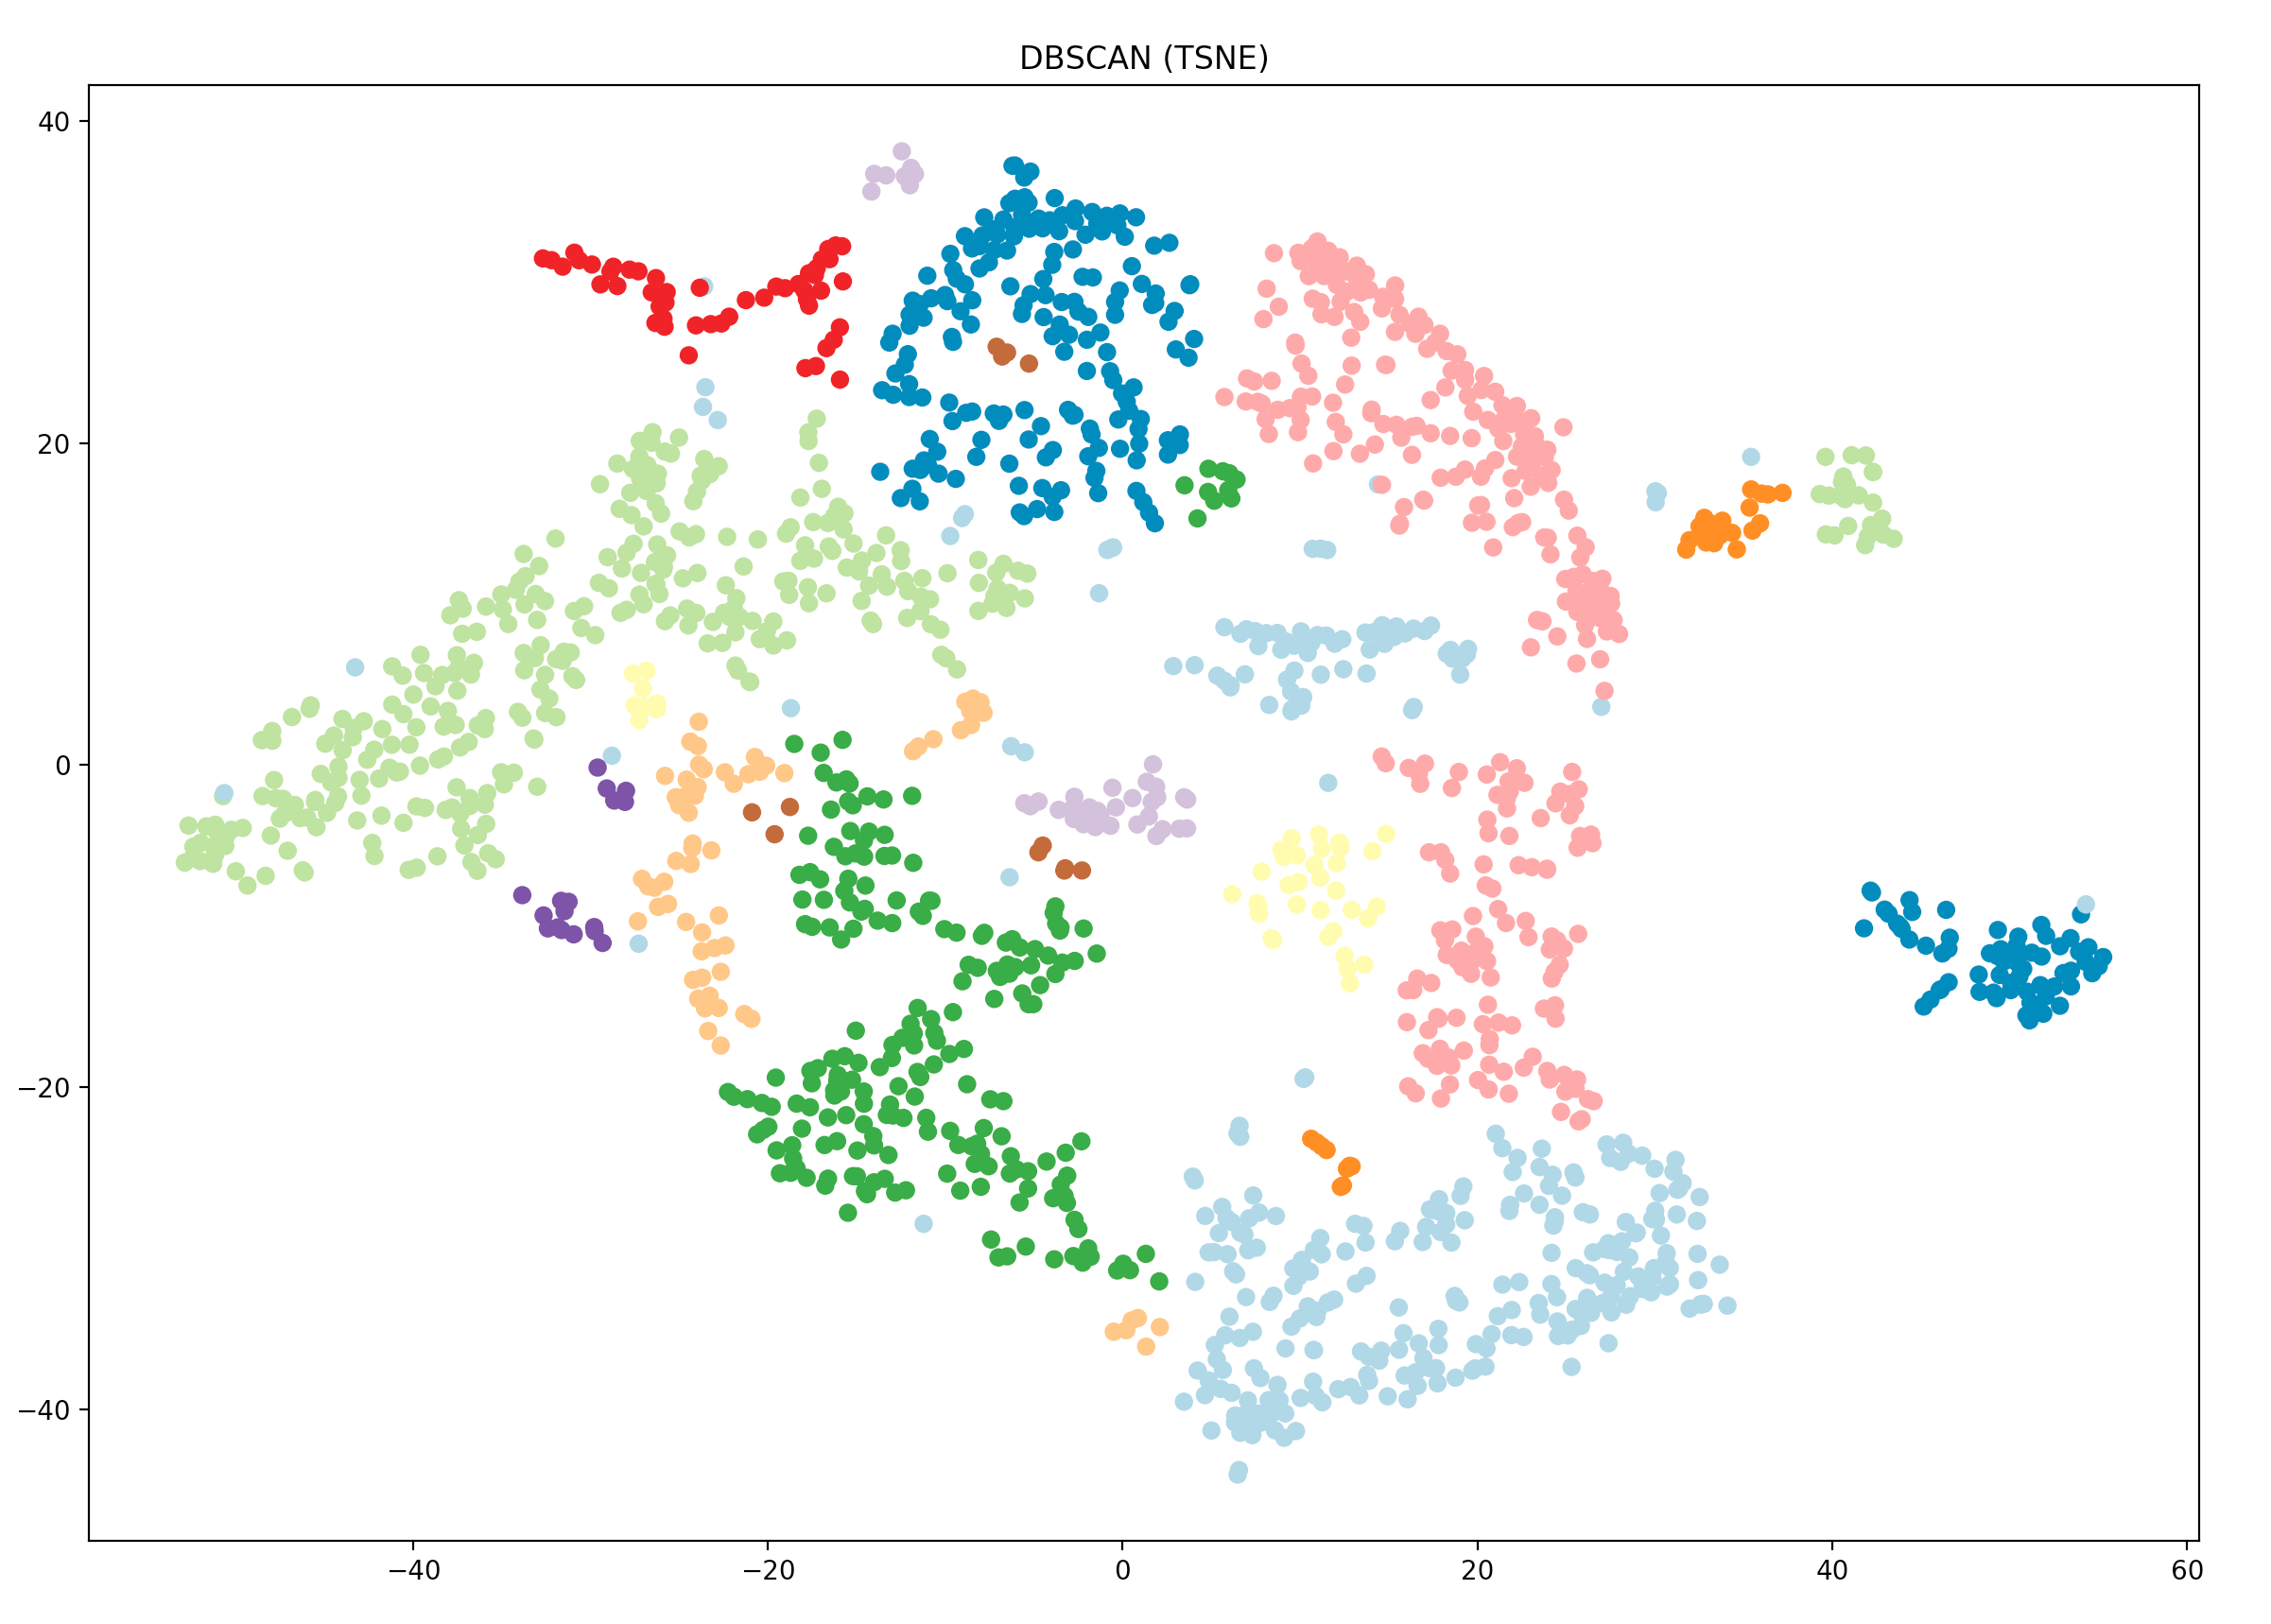
\includegraphics[width=0.9\textwidth]{./images/tsneParametersTest/1h-1-finalTSNEDBSCAN.png}
	\end{subfigure}
	\caption{Final t-SNE parameters (1h data files): perplexity=40, learning\_rate=20, n\_iter=5000 }
  \label{figure:finalTSNE1h}
\end{figure}

\begin{figure}
  \centering
	\begin{subfigure}{.5\textwidth}
    \centering
    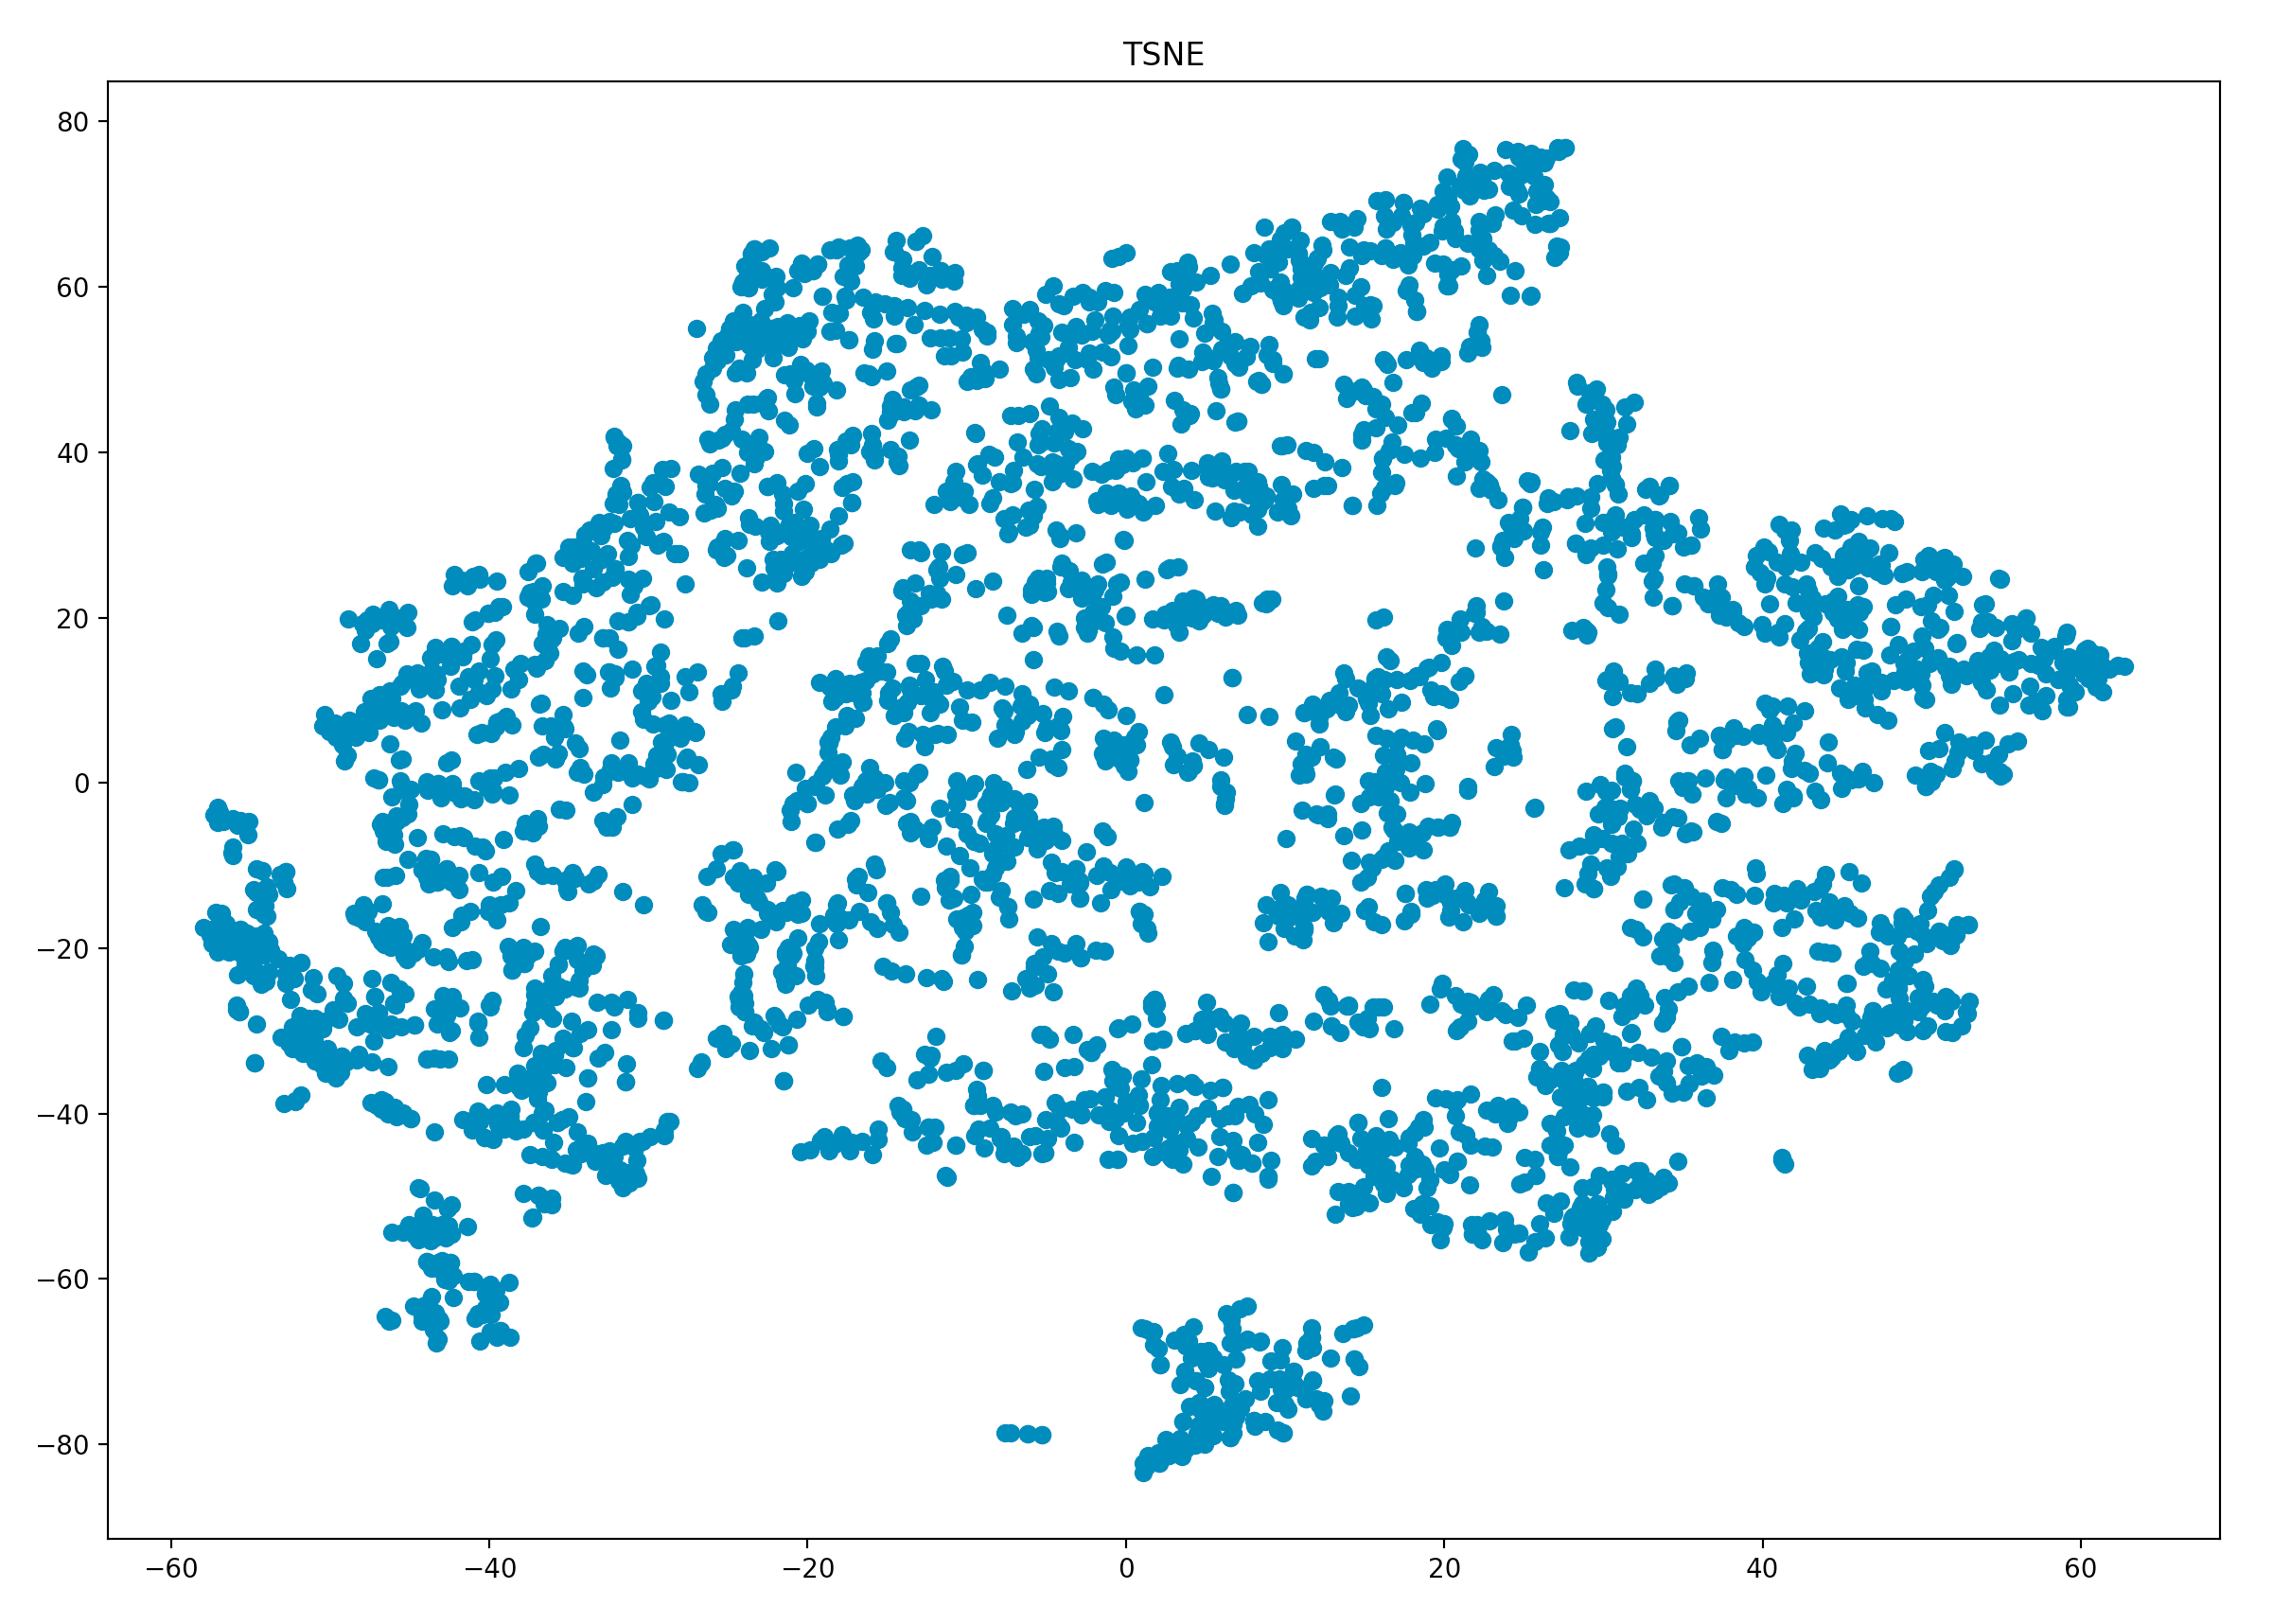
\includegraphics[width=0.9\textwidth]{./images/tsneParametersTest/3h-1-finalTSNE.png}
  \end{subfigure}%
  \begin{subfigure}{.5\textwidth}
    \centering
    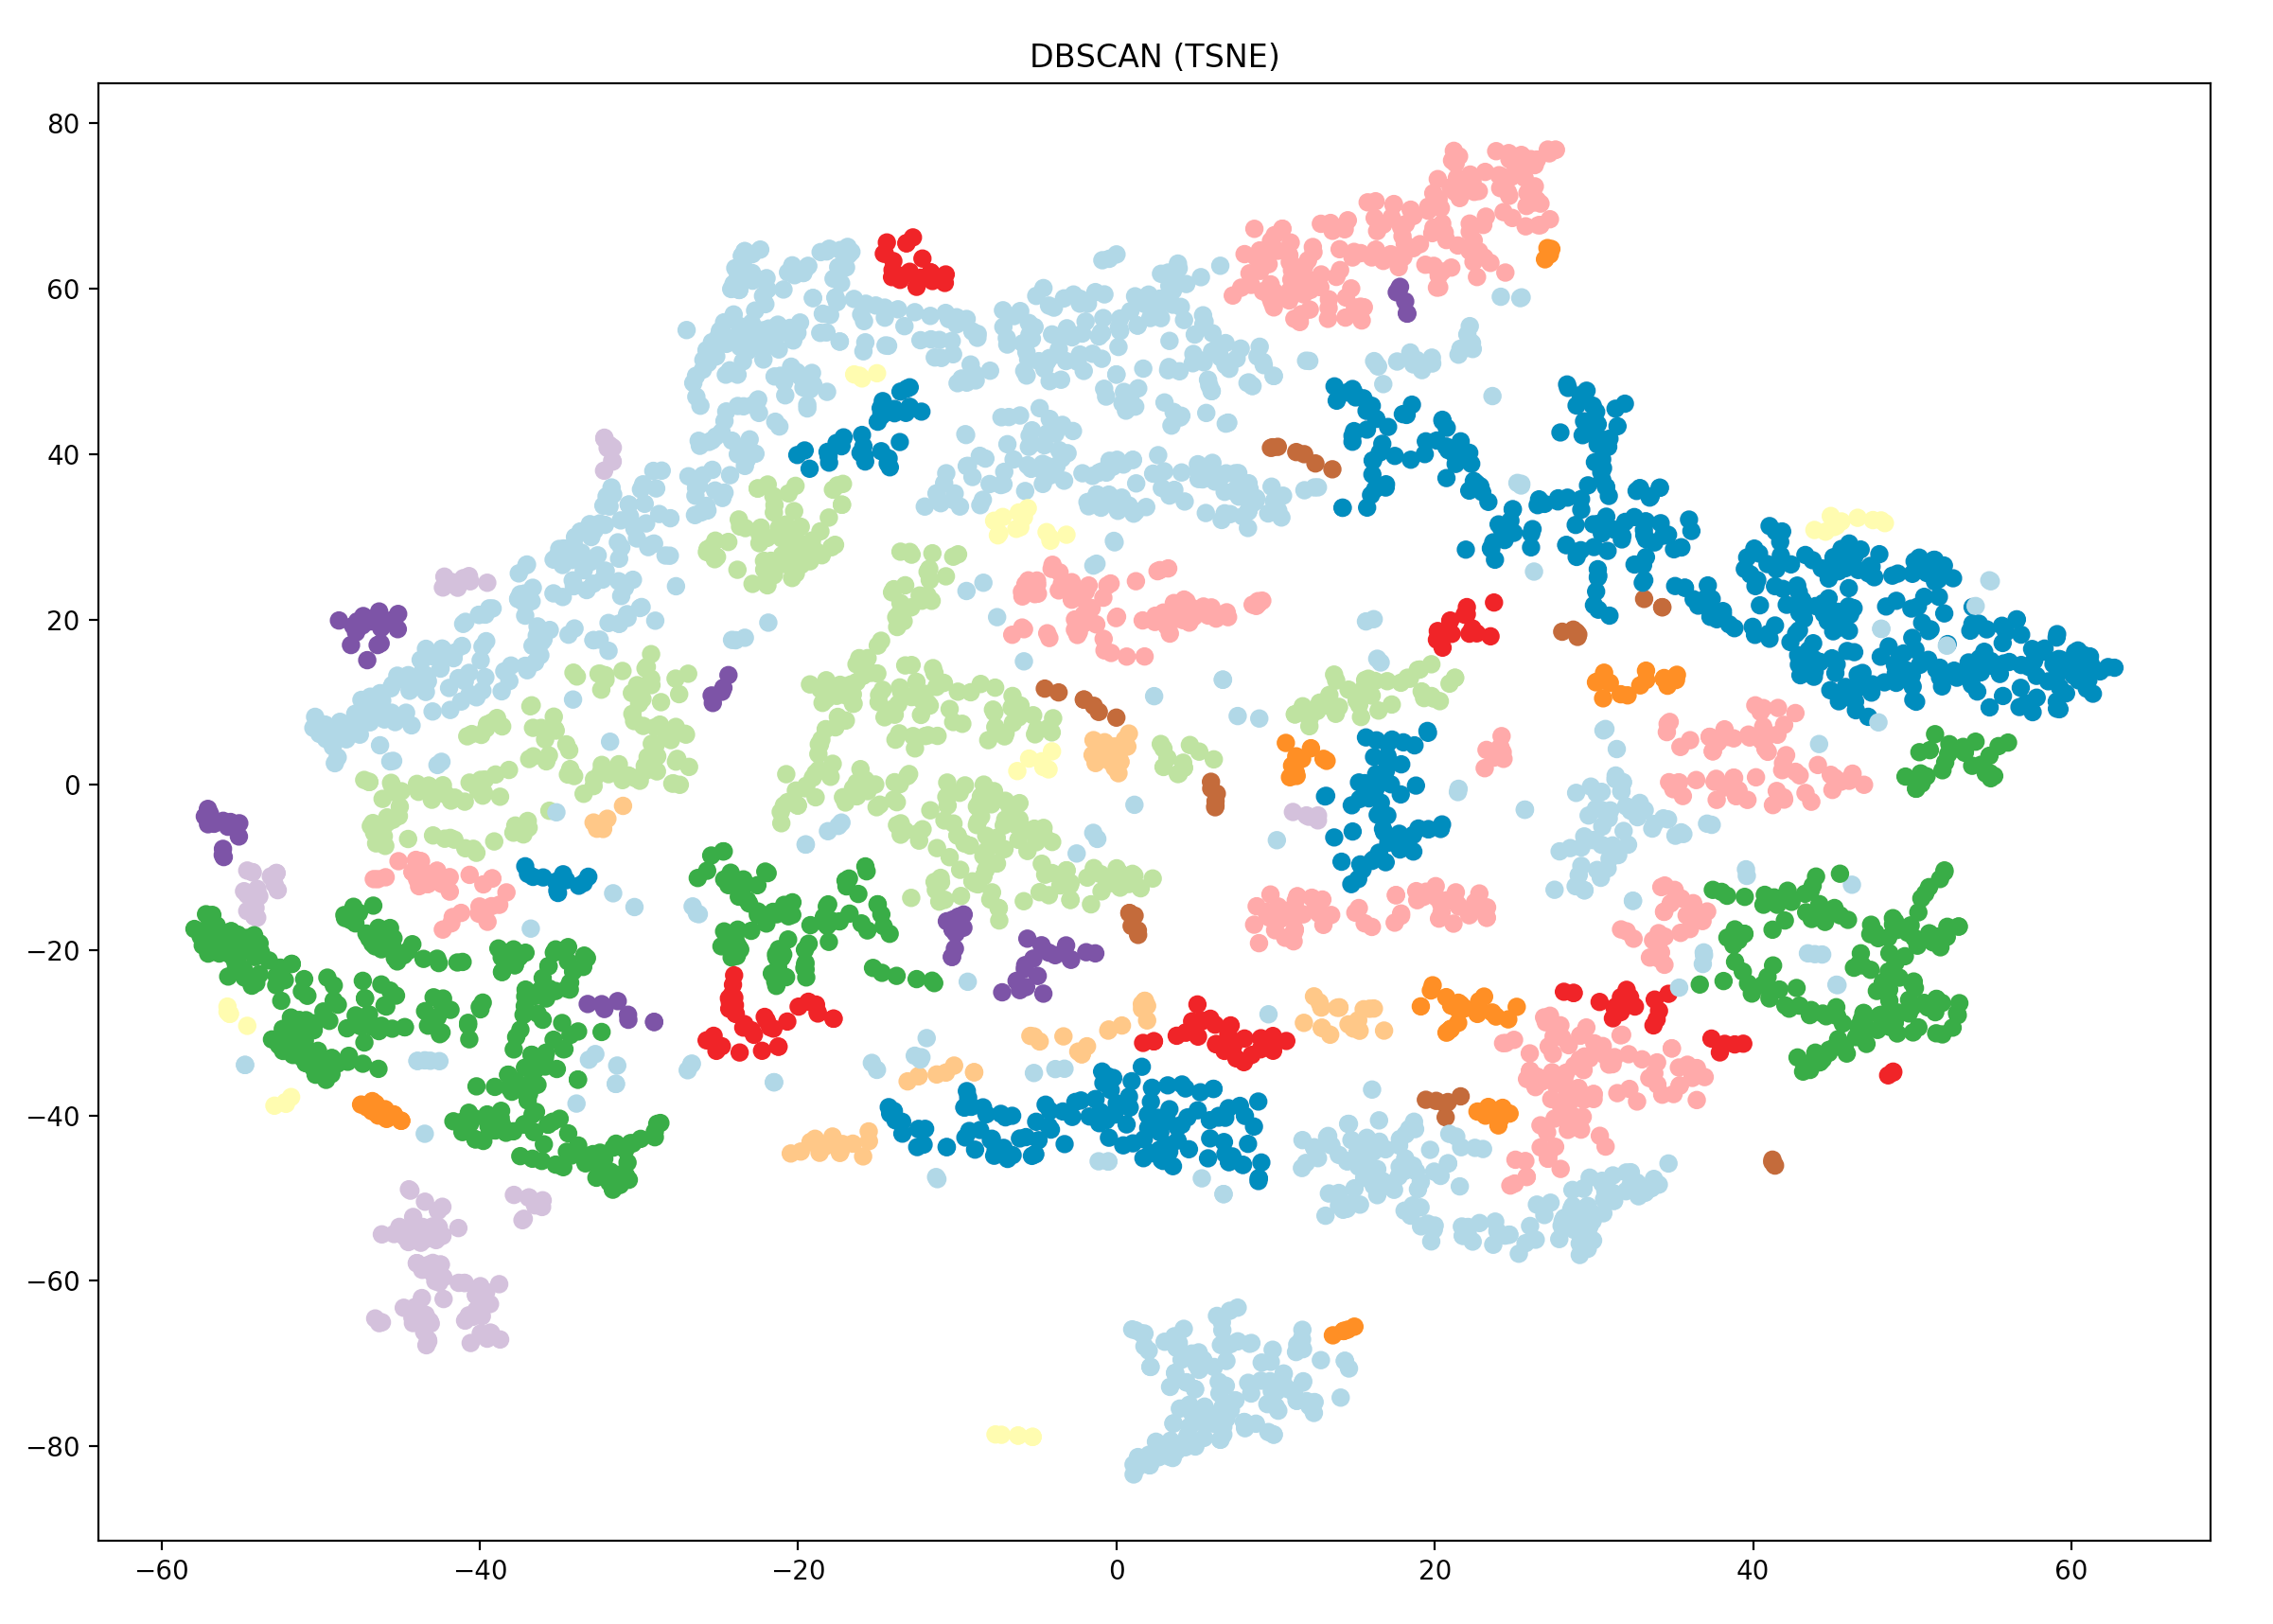
\includegraphics[width=0.9\textwidth]{./images/tsneParametersTest/3h-1-finalTSNEDBSCAN.png}
	\end{subfigure}
	\caption{Final t-SNE parameters (3h data files): perplexity=40, learning\_rate=20, n\_iter=5000}
  \label{figure:finalTSNE3h}
\end{figure}



  \subsection{Clustering}
  \label{section:ExperimentClustering}
  The clustering algorithms used for the SmartEater data set, were DBSCAN and OPTICS. One of the advantages of these density-based clustering methods (as mentioned in section \ref{section:densityBasedMethods}) are that there are less parameters to configure. Another reason for choosing these methods, is that there is no need to define a fixed number of \textit{k} clusters to find, since the cluster boundaries are regulated by density. This technique also allows to arbitrary-shaped clusters to be correctly identified.

\subsubsection{DBSCAN}
The DBSCAN algorithm was applied on the SmartEater data set using the sklearn DBSCAN\footnote{\url{https://scikit-learn.org/stable/modules/generated/sklearn.cluster.DBSCAN.html}} function.
Section \ref{section:DBSCAN} describes the functionality of the DBSCAN clustering method. As mentioned, one of the disadvantages of DBSCAN, is the need to specify parameters, which can change the outcome of the results. In order to establish suitable parameters, k-dist graphs were generated for the 1h and 3h data sets. The graphs contained the distances to the k nearest neighbors. As recommended by \textcite{DBSCAN}[230], MinPts and \textit{k} were set to 4 and the graphs were used to determine Eps. The idea is to select Eps suitable for the "thinnest" cluster, however being careful to avoid noise. As can be seen in figures \ref{figure:kDistGraphDBSCAN1h} and \ref{figure:kDistGraphDBSCAN3h}, the valley starts at roughly a 4th nearest neighbor distance of 2. 

% \begin{figure*}[h]
%   \centering
%   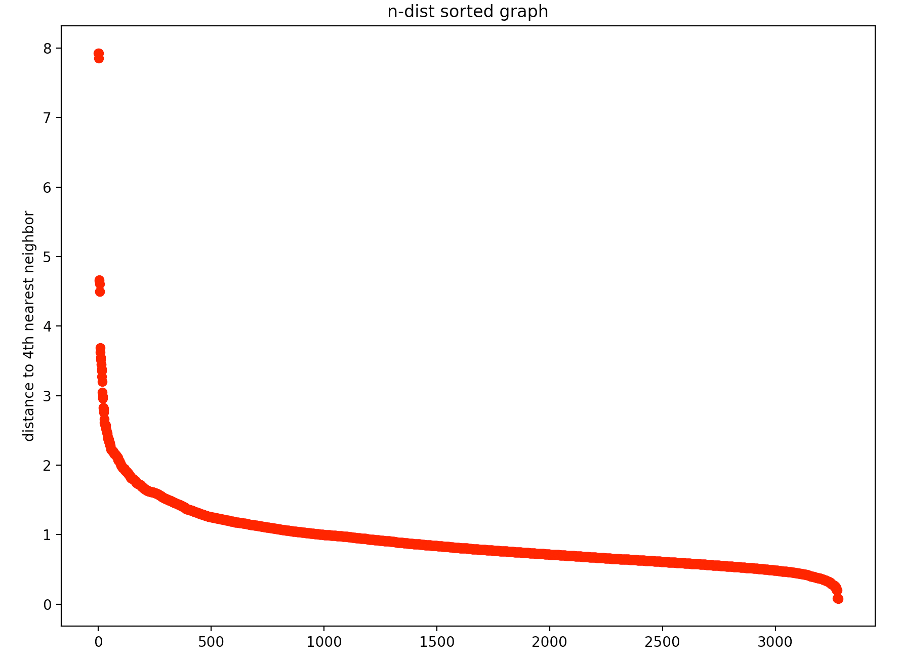
\includegraphics[width=0.5\textwidth]{./images/kDistGraphDBSCAN1h.png}
%   \caption{Sorted 4-dist graph of the 3h data set (distance for each point to its fourth nearest neighbor). The valley starts at roughly the 4th nearest neighbor distance of 2.}
%   \label{figure:kDistGraphDBSCAN1h}
% \end{figure*}

% \begin{figure*}[h]
%   \centering
%   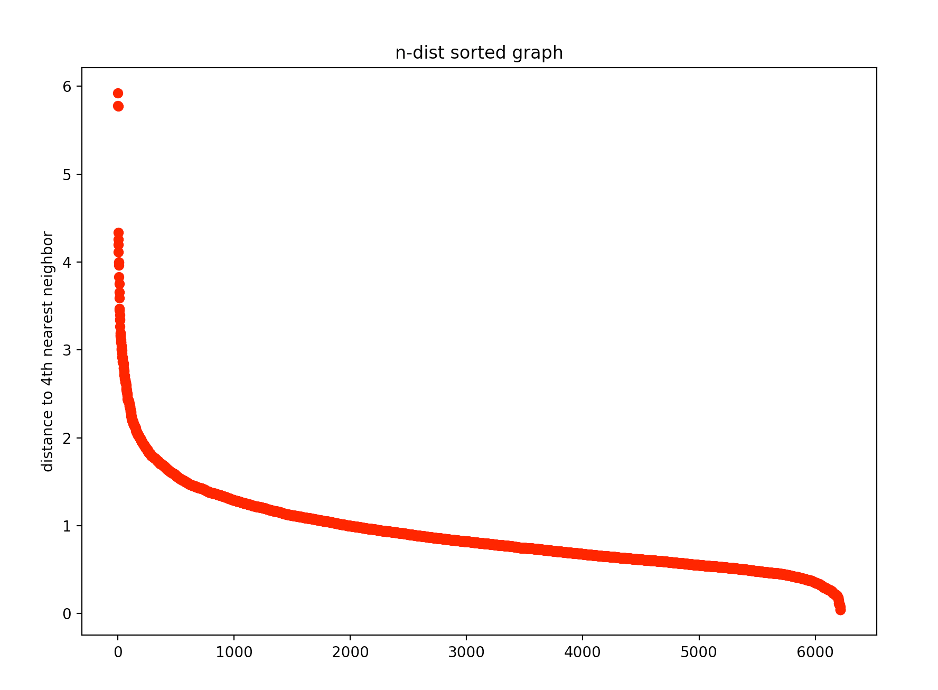
\includegraphics[width=0.5\textwidth]{./images/kDistGraphDBSCAN3h.png}
%   \caption{Sorted 4-dist graph of the 1h data set (distance for each point to its fourth nearest neighbor). The valley starts at roughly the 4th nearest neighbor distance of 2.}
%   \label{figure:kDistGraphDBSCAN3h}
% \end{figure*}


\begin{figure}
  \centering
  \begin{subfigure}{.5\textwidth}
    \centering
    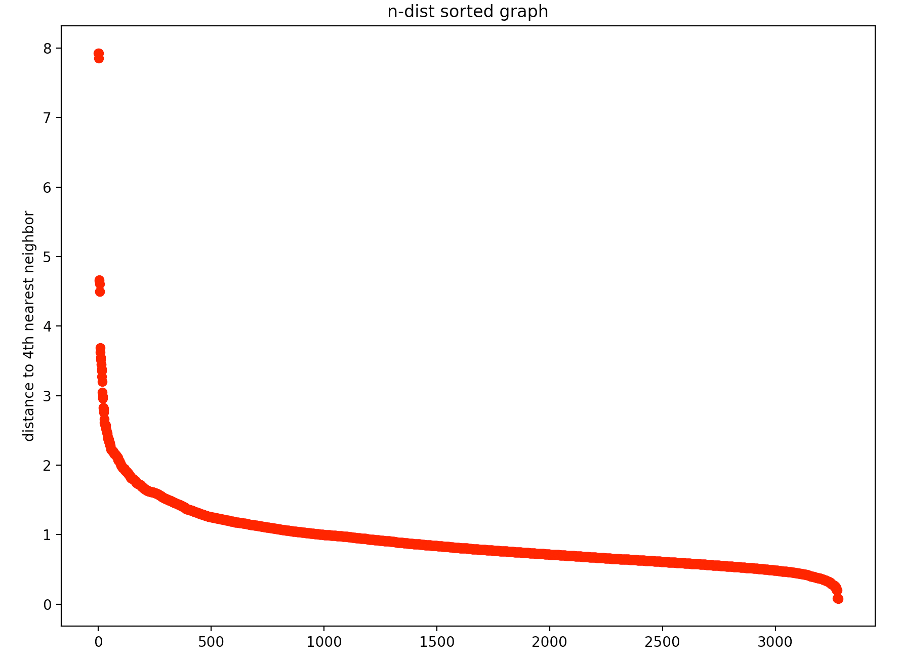
\includegraphics[width=0.87\textwidth]{./images/kDistGraphDBSCAN1h.png}
  \caption{1h dataset}
  \label{figure:kDistGraphDBSCAN1h}
  \end{subfigure}%
  \begin{subfigure}{.5\textwidth}
    \centering
    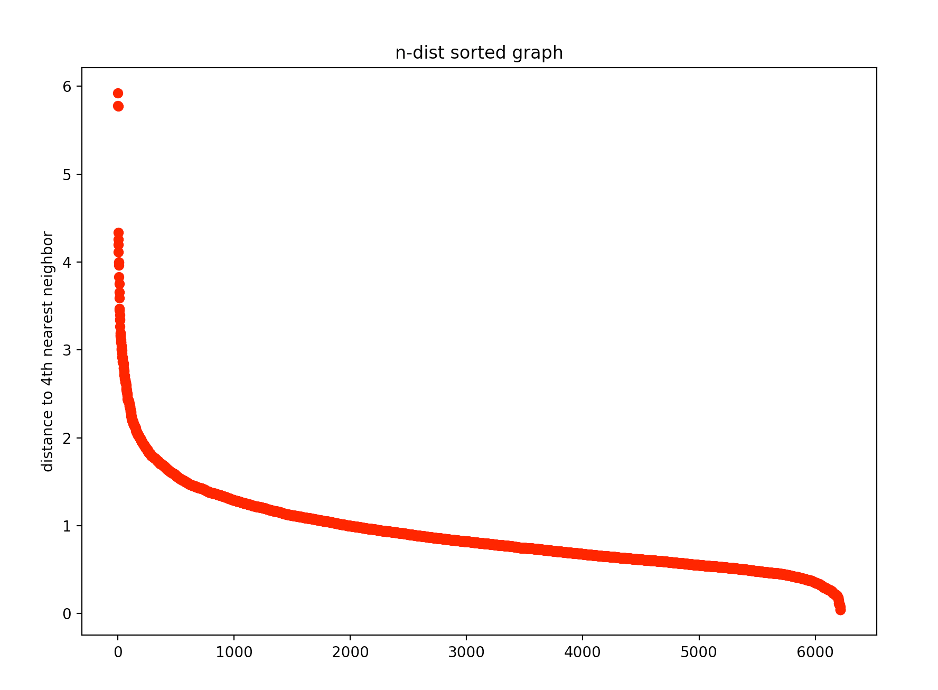
\includegraphics[width=1\textwidth]{./images/kDistGraphDBSCAN3h.png}
    \caption{3h data set}
    \label{figure:kDistGraphDBSCAN3h}
  \end{subfigure}
  \caption{Sorted 4-dist graphs (distance for each point to its fourth nearest neighbor), used to determine a suitable Eps parameter for the DBSCAN algorithm. The valley starts at roughly the 4th nearest neighbor distance of 2, therefore Eps should be 2.}
  \label{figure:kDistGraphDBSCAN}
  \end{figure}

The DBSCAN method applied, with the parameters eps = 2 and min\_samples (MinPts) = 4.  The results of this clustering method can be seen in \textbf{TODO: FIGURES}.



\subsubsection{OPTICS}
The OPTICS algorithm was also implemented with its sklearn function\footnote{\url{https://scikit-learn.org/stable/modules/generated/sklearn.cluster.OPTICS.html}}. As stated in section \ref{section:OPTICS}, the OPTICS algorithm creates a reachability plot for the data points. The plots created for the SmartEater data files are depicted in \textbf{TODO FIGURES}. Initially, the clusters were extracted using the clustering method "xi". This is the automatic cluster extraction method, as explained in section \ref{section:OPTICS} and in \textcite{OPTICS}[57]. The visual results of these clusterings contained a lot of noise ??? \textbf{todo, show both xi and dbscan comparison, and explain why, also show silhouette, ... scores to prove that dbscan method provided better clusters}





% optics: two options: xi (automatic technique from \textcite{OPTICS}, or dbscan)







  \subsection{Comparison and Evaluation of clusters of different time lengths}
  \label{section:ExperimentComparisonTimeLengths}
  
The three mathematical evaluation scores mentioned in section \ref{section:TheoryEvaluatingClusteringResults}, i.e. Silhouette Coefficient, Davies-Bouldin Index, and Caliński-Harabasz Index, were used to compare the resulting clusters.  They were each implemented using the sklearn library, the same way as in section \ref{section:experimentTSNE}. These three scores were calculated and stored for each DataFrame, after each clustering algorithm was applied (DBSCAN and OPTICS) for each time length. The resulting values were then compared and are detailed in this section.

The experiment was run on each time length (\textit{1h files:} 15 min, 30 min, 45 min, 1h; \textit{3h files:} 30 min, 1h, 1 h 30 min, 2h, 2h 30 min, 3h).
The numbers were different for each time the results were calculated, since t-SNE produces slightly different results. Therefore, the t-SNE and clustering was run multiple times and the results were compared. In figures \ref{figure:clusteringResults1} and \ref{figure:clusteringResults2}, two individual t-SNE and clusterings were run, figure \ref{figure:clusteringResults3} depicts the average scores of these two. Figure \ref{figure:clusteringResults4} depicts an average of a different two runs. These mentioned runs all held the learning rate parameter 20. Since a learning rate of 800 also proved to be a viable choice, the t-SNE and clustering was also run twice and averaged with this learning rate (figure \ref{figure:clusteringResults5}). These figures (\ref{figure:clusteringResults1} to \ref{figure:clusteringResults5}) are located in appendix \ref{appendix:clusteringEvaluationResults}. The mean was taken from all these results, thus creating figure \ref{figure:clusteringResults6}. From these, there is no clear winner, although there are some stronger candidates, i.e. 15 min (1h), 1h (1h), and 2h (3h). 

Like in section \ref{section:experimentTSNE}, when comparing the t-SNE results, the green fields from all the above mentioned results, or number of wins, were summed to see which time length had the best number of scores the most times. The wins per dataset (1h or 3h - all green fields) for the 1h data files are pictured in figure \ref{figure:clusteringResultsGraph1h}, in figure \ref{figure:clusteringResultsGraph3h} for the 3 hour data files. The two top winners for the 1h data files and the 3h data files, were: 15 min (1h), 30 min (1h), 2h (3h), and 1h (3h). Figure \ref{figure:clusteringResultsGraphTotal} shows the comparison of the dark green wins (1h and 3h). The top four results were: 30 min (1h), 1h (3h), 2h (3h), and 30 min (3h). The number of wins is to some extent reliable on the resulting scores from other time lengths it happened to be compared with. It also does not fully factor in the full extent of how far this time length was better. For this reason, time lengths that were among the stronger candidates at least once (either in figures \ref{figure:clusteringResults6}, \ref{figure:clusteringResultsGraph1h} and \ref{figure:clusteringResultsGraph3h}, or \ref{figure:clusteringResultsGraphTotal}) were compared solely to each other. The results are detailed in figure \ref{figure:clusteringResults8}. The 2h time delta achieved the majority of best scores in this final comparison. 

\begin{figure}
  \centering
  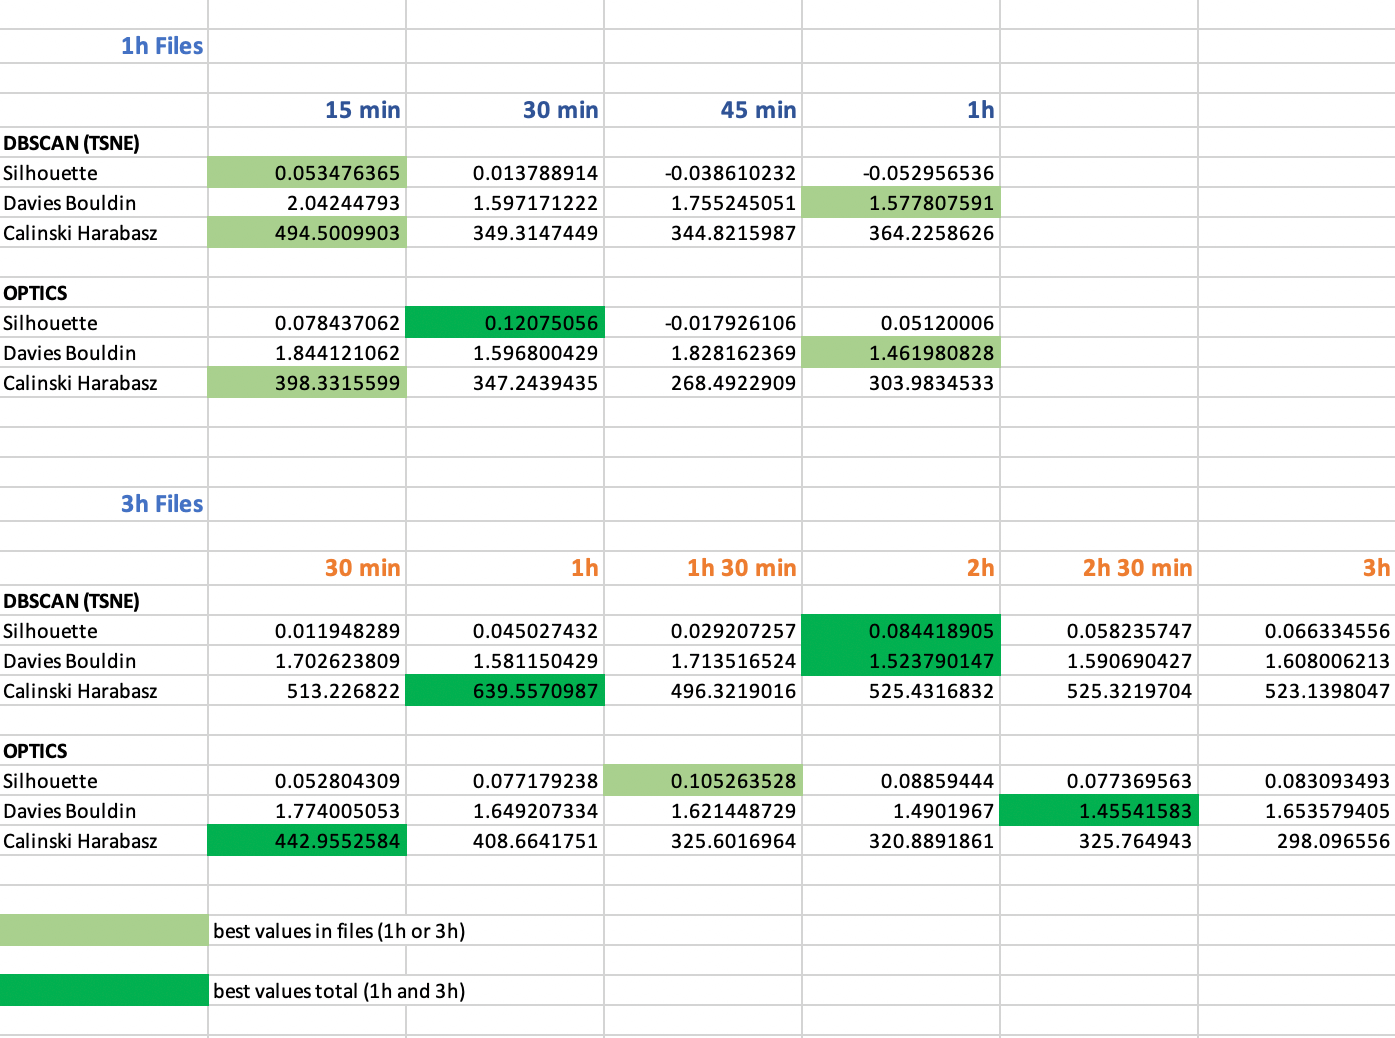
\includegraphics[width=0.8\textwidth]{./images/clusteringResults/clusteringResults6.png}
  \caption{Evaluation scores comparison averaged from figures \ref{figure:clusteringResults1}, \ref{figure:clusteringResults2}, \ref{figure:clusteringResults3}, \ref{figure:clusteringResults4}, and \ref{figure:clusteringResults5} (located in appendix \ref{appendix:clusteringEvaluationResults}). The green highlighted values indicate the best achieving evaluation score values (1h or 3h files), for the corresponding clustering method. Furthermore, the dark green highlighted values also accentuate the overall best scoring values over all datasets (1h and 3h files).}
  \label{figure:clusteringResults6}
\end{figure}


\begin{figure}
  \centering
  \begin{subfigure}{.475\textwidth}
    \centering
    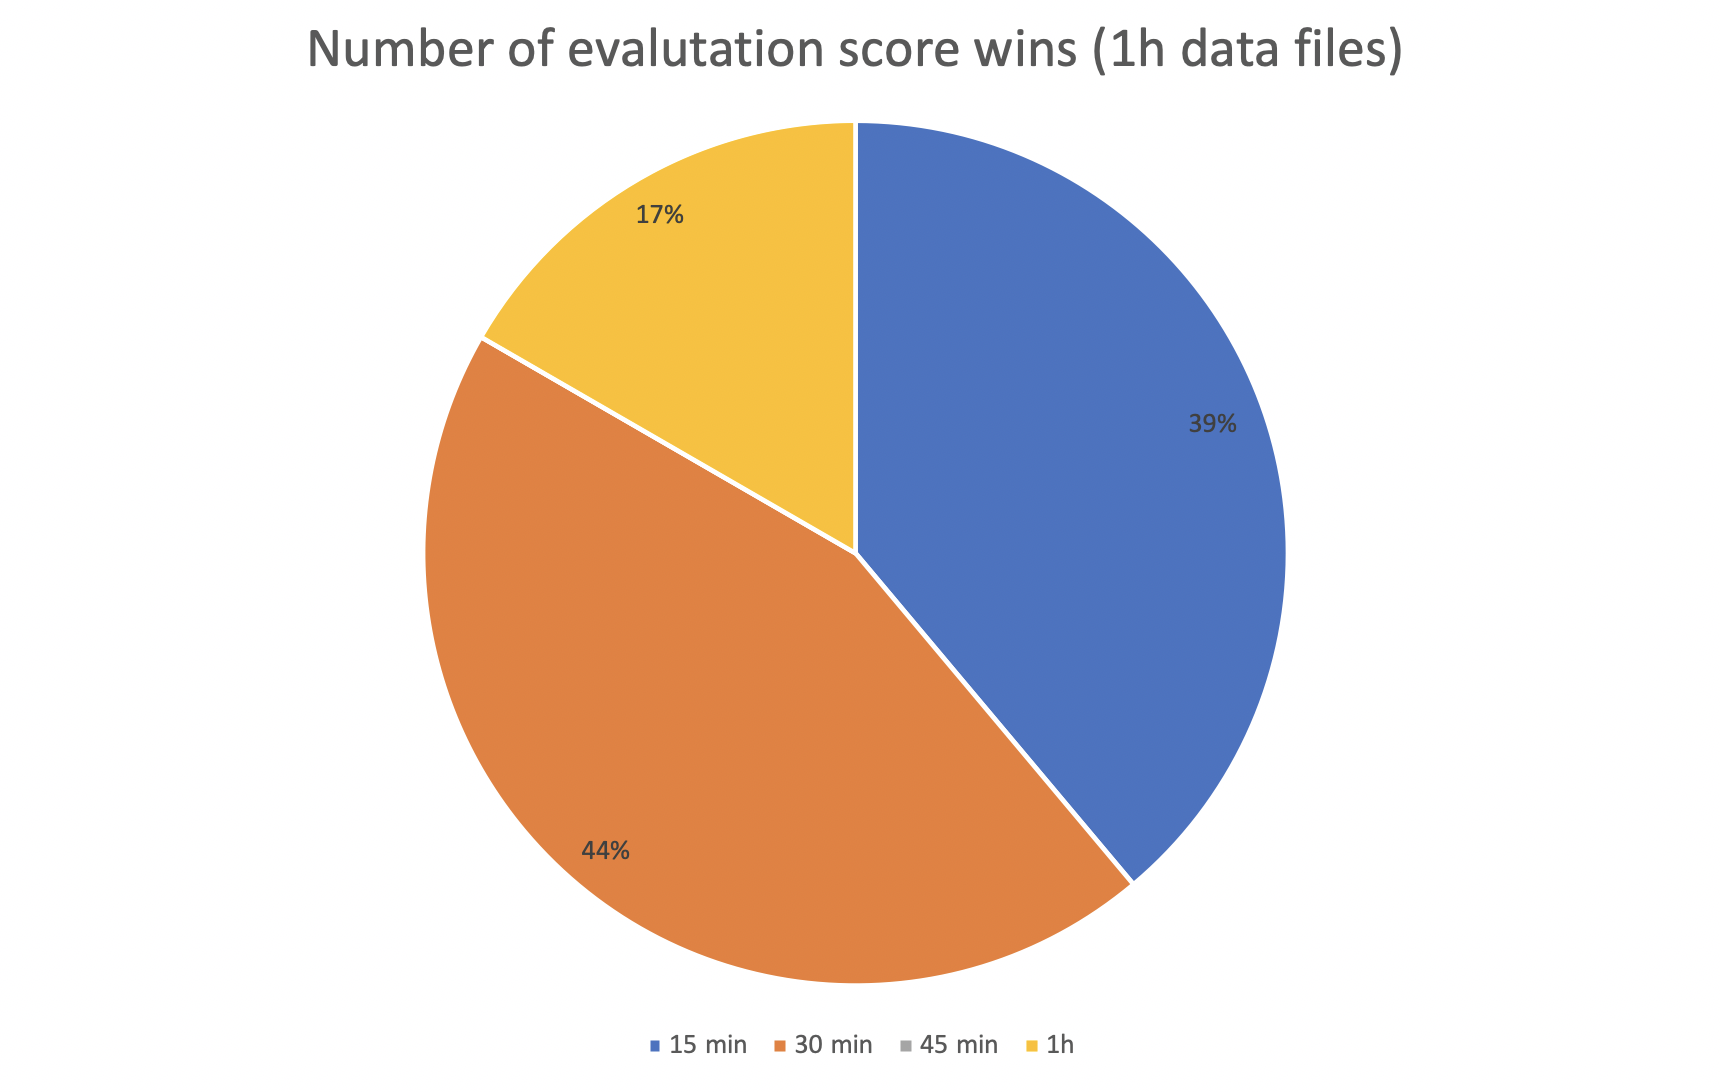
\includegraphics[width=1\textwidth]{./images/clusteringResults/clusteringResultsGraph1h.png}
    \caption{Number of evaluation score wins (1h or 3h dataset) for the 1h data files.}
    \label{figure:clusteringResultsGraph1h}
  \end{subfigure}
  \hfill
  \begin{subfigure}{.475\textwidth}
    \centering
    \  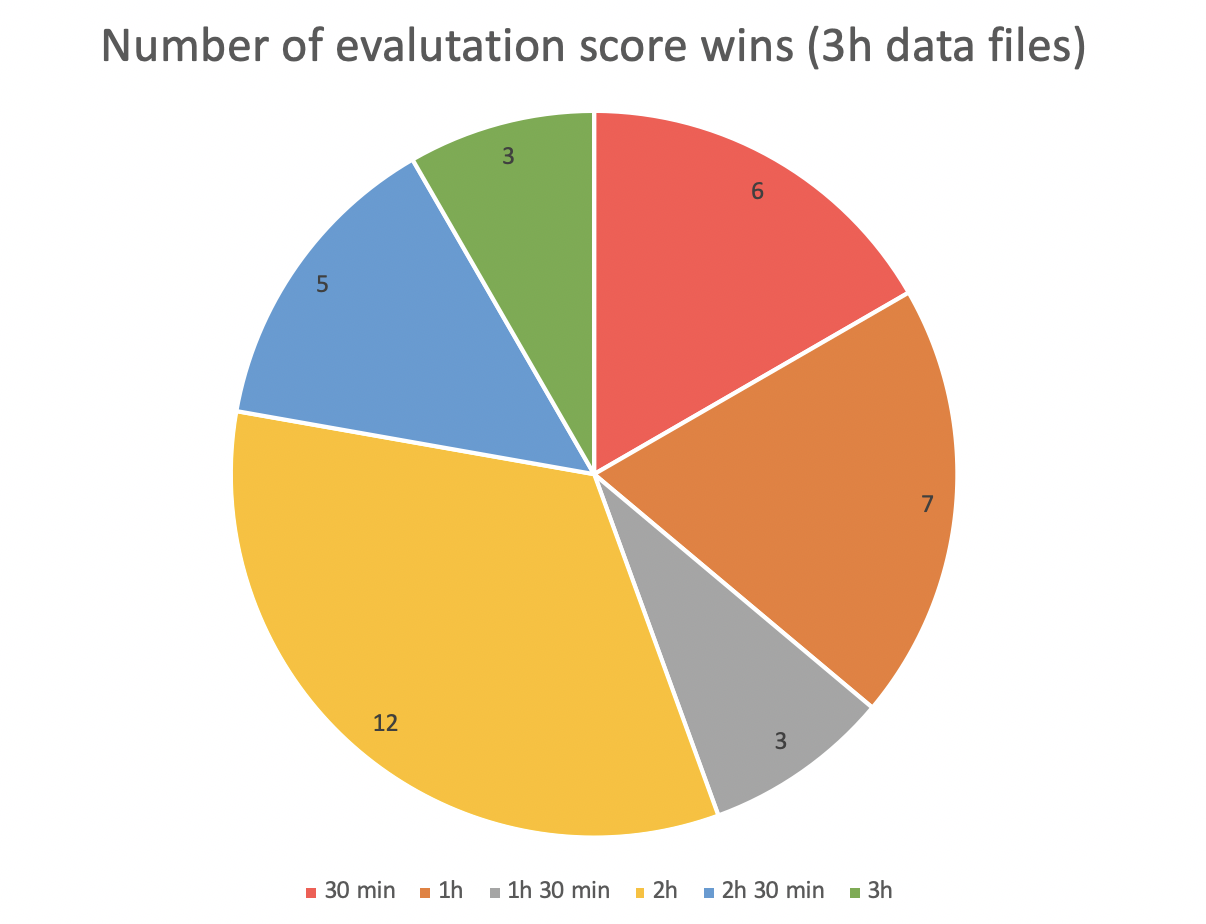
\includegraphics[width=1.2\textwidth]{./images/clusteringResults/clusteringResultsGraph3h.png}
    \caption{Number of evaluation score wins (1h or 3h dataset) for the 3h data files.}
    \label{figure:clusteringResultsGraph3h}
  \end{subfigure}
\end{figure}

\begin{figure}
  \centering
  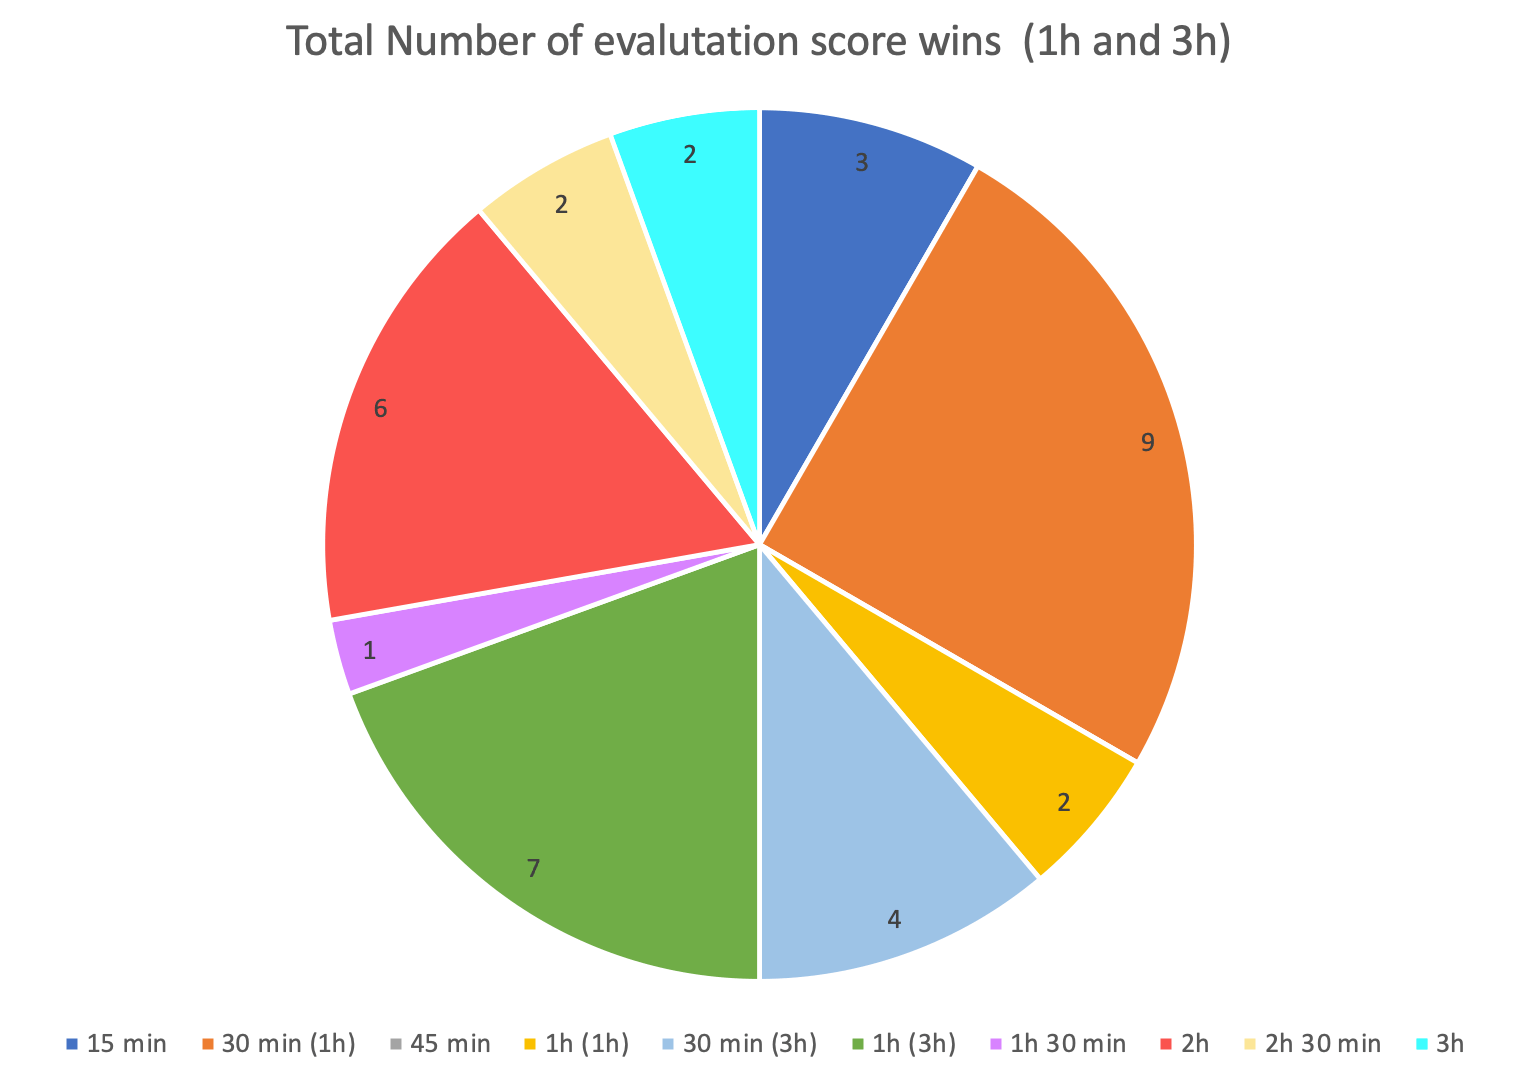
\includegraphics[width=0.7\textwidth]{./images/clusteringResults/clusteringResultsGraphTotal.png}
  \caption{Number of dark green evaluation score wins (overall wins in 1h and 3h dataset).}
  \label{figure:clusteringResultsGraphTotal}
\end{figure}

\begin{figure}
  \centering
  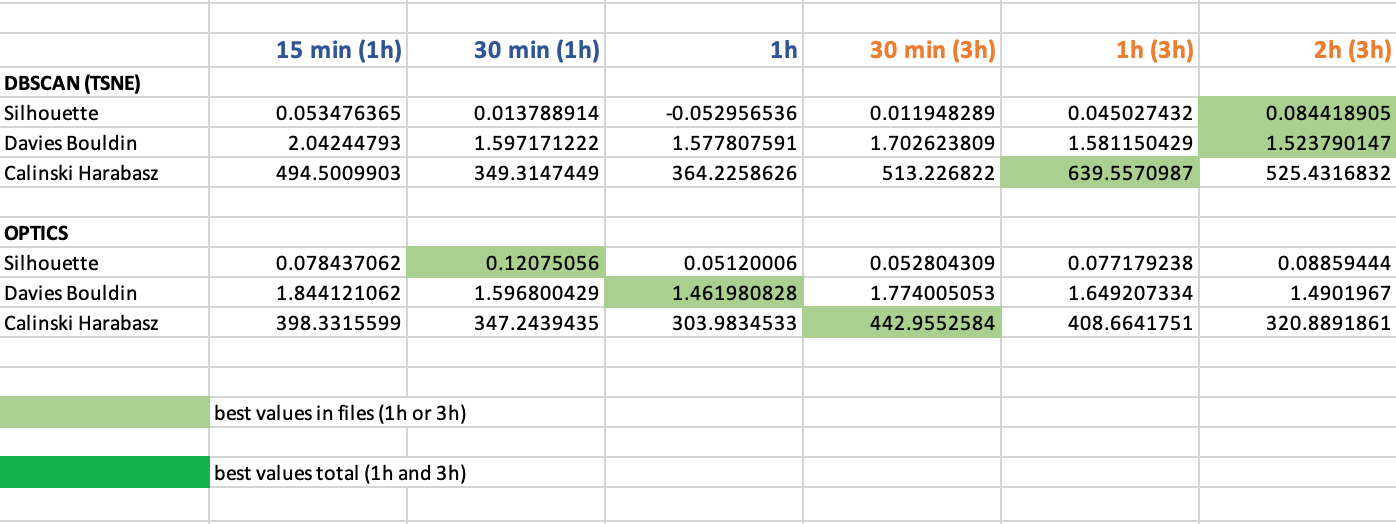
\includegraphics[width=0.8\textwidth]{./images/clusteringResults/clusteringResults8.png}
  \caption{Comparison of top evaluation score performers (of clusterings) from figures \ref{figure:clusteringResultsGraph1h}, \ref{figure:clusteringResultsGraph3h}, and \ref{figure:clusteringResultsGraphTotal}. The light green highlighted cells indicate the best value across the different time lengths for that score.}
  \label{figure:clusteringResults8}
\end{figure}

\clearpage

  
  \subsubsection{Mathmatical Evaluation}
  % \label{section:TheoryEvaluatingClusteringResults}
  % The resulting clusters received from the previously mentioned clustering algorithms are assessed in the \textit{cluster evaluation} step. \textcite{han2011data}[396, 398] describe this stage as assessing the quality of the results.
There are different steps to be taken in evaluating clusters, e.g. evaluation of the cluster quality, assessment of the cluster tendency (whether non random stuctures exist), and establishing the number of clusters (e.g. for k-means clustering). The experiment described in this thesis used mathmathical evaluation methods to compare cluster quality among the different time lengths. 
 
  % \subsubsection{Assessment of the cluster tendency}
  % As explained by \textcite{han2011data}[396-397], the tendency must be assessed, meaning it is tested, whether structures exist that aren't random. Running a clustering algorithm on any dataset will return clusters. However, only non random structures are significant and not misleading. For example, if a dataset consists of data points that are uniformly distributed, if a clustering algorithm delivers clusters, these will be random and have no purpose. Spatial randomness tests (e.g. Hopkins Statistic) can be used to measure how likely the data was created by uniform data distribution.

 

  % \subsubsection{Evaluation of the cluster quality}
  % (\textbf{Todo: adjust to the methods used in the experiment})

  \textcite{han2011data}[399, 401] mention, that the cluster quality needs to be evaluated. Generally, there are two ways to measure the quality of clustering: extrinsic methods and intrinsic methods. In extrinsic methods, there is a ground truth available, therefore these are also referred to as supervised methods. This ground truth is usually produced by experts (humans). Intrinsic methods are used, when there is no ground truth available. In intrinsic methods, the clusters are evaluated by how well they are separated from one another and how compact they are (e.g. \textit{silhouette coefficient}).
  % NOT SURE IF SHOULD EXPLAIN EXTRINSIC, SINCE DON'T THINK USING.
  The experiment described in this paper uses intrinsic methods, since there is no ground truth for comparison.
  
  
  \paragraph{Silhouette Coefficient}
  \label{section:silhouetteCoefficient}
  In his paper, \textcite{rousseeuw1987silhouettes}[53-57, 59] proposes a new graphical display using silhouettes, to help determine how well objects belong to their assigned clusters. It can be used to interpret and validate the results of clustering. It is also utilised to compare the resulting clusters with those output using alternative algorithms (the input data being the same). 
  
  % In an example, where countries are assigned a value of how dissimilar they are to another country, the results are listed in a table. A structure contained in the results (consisting of 66 numbers), is hard to identify. Therefore, the countries are categorised into clusters using k-median. It is however uncertain, whether the clusters follow a specific structure, or if the groups are simply artificial. 
  % With the use of silhouettes, the author's goal is to answer the following questions: Is the quality of the clusters high, therefore the dissimilarities of the objects within a cluster are small, and large compared to the objects in other clusters? Are the objects well-classified, misclassified and which ones were not classified (between clusters)? Is it possible to perceive which "natural" clusters are available in the dataset?
  %According to Rousseeuw, the silhouettes are ideal when the distance between objects are on a ratio scale (e.g. Euclidean distances) and when the goal is to receive clear and compact clusters.

  The formula is as follows:
  With the use of silhouettes, the author's goal is to find out, if the quality of the clusters is high. Hence, the dissimilarities of the objects within a cluster are small, and the dissimilarities are large compared to the objects in other clusters. For each object \textit{i} (in cluster \textit{A}) the value \textit{s(i)} is calculated. \textit{a(i)} contains the average dissimilarity of the object \textit{i} to each other object in the same cluster. If there are no other objects in the cluster, \textit{s(i)} is set to zero (most neutral value). \textit{b(i)} is determined by firstly calculating the average dissimilarity for each neighbouring cluster that isn't \textit{A}. The shortest of these values, therefore the next closest cluster to \textit{A}, is then assigned to \textit{b(i)}. This cluster can so to say be seen as the next best choice for \textit{i}. \textit{b(i)} can only be calculated, if there are other clusters beside \textit{A}. The formula for \textit{s(i)} is as follows:
  \[
    s(i) = \frac{b(i) - a(i)}{max\{a(i), b(i)\}}  
  \]
  The resulting value \textit{s(i)} is a number in the range of \textit{-1 $\leq$ \textit{s(i)} $\leq$ 1}:

  \[ s(i) =
  \begin{cases}
    1 - a(i)/b(i)       & \quad \text{if } a(i) < b(i)\\
    0       & \quad \text{if } a(i) = b(i)\\
 b(i)/a(i) - 1      & \quad \text{if } a(i) > b(i)

  \end{cases}
\]
A \textit{s(i)} value close to 1 reveals, that the dissimilarity within a cluster is smaller than the dissimilarity to the neighbouring cluster. Therefore it suggests, that the assignment of that object is good, since it is most likely the most suitable cluster for \textit{i} (well-classified). A \textit{s(i)} value close to 0 means that \textit{a(i)} and \textit{b(i)} are almost equal and it is uncertain whether cluster \textit{A} or its neighbour is a more suitable fit. If \textit{s(i)} is near -1, then the dissimilarity within a cluster is larger than the dissimilarity to the next closest cluster. Thus, it would have been more natural to assign \textit{i} to the neighbouring cluster, since it is closer to it (misclassified).

The \textit{average silhouette width} can be calculated for single clusters. It is received by calculating the average of all objects that belong to said cluster. An average score can also be calculated from each object \textit{i} for the whole chart (dataset), the so called \textit{overall average silhouette width}. 

% \textcite{silhouetteRelocatingMeasure}[15] use the silhouette coefficient in their proposed clustering algorithm, which clusters categorical data. The coefficient was used assess the quality of the clusters and to relocate objects to more fitting clusters. The cluster efficiency in their algorithm was therefore enhanced.



% %TODO: there is some more about it with examples - but not sure if need - from p. 584

\paragraph{Davies-Bouldin Index}
A second cluster evaluation method is the Davies-Bouldin Index, which was announced by \textcite{DaviesBouldin}[224-227]. 
% The goal is to calculate the average similarity of a cluster with the cluster that is most similar to it. 

The succeeding formula describes the average similarity of a cluster with the cluster that is most similar to it (\textit{R\textsubscript{ij}} ).
\textit{i} and \textit{j} represent the determined clusters, \textit{S\textsubscript{i}} and \textit{S\textsubscript{j}} stand for the dispersions of the clusters, and \textit{M\textsubscript{ij}} is the distance between the two cluster centroids. 

\[
  R_{ij} = \frac{S_i + S_j}{M_{ij}}  
\]

The Davies-Bouldin Index equals:
\[
\overline{R} = \frac{1}{N}\sum_{i=1}^{N}R_i
\]

This metric can be used, to compare clustering results. The lower of the two \textit{\=R} values indicates the better partitioning.

\paragraph{Caliński-Harabasz Index}
As a third evaluation score, \textcite{calinskiHarabasz}[3, 7, 11, 23, 24, 26] is used to evaluate and compare the resulting clusters in the experiment. 
The Caliński-Harabasz Index or Variance Ratio Criterion (VRC) is calculated as 
% follows, where \texit{n} is the number of points \textit{k} is the number of clusters, \textit{WGSS} is the within-group (cluster) sum of squares, and \textit{BGSS} is the between-group (cluster) sum of squares.
\[
VRC = \frac{BGSS}{k-1}/\frac{WGSS}{n-k}
\]
If \textit{k} is not known, it is set to 2, then 3 and so on. The density of the clusters can be calculated with the sums of the squared distances from the cluster centroids, to the points. The more natural the clusterings are, the higher VRC will be, since the variation within the cluster is lower.


%Determining the minimum of WGSS can be utilised for cluster analysis.



% \subsubsection{Establishing the number of clusters}
%  \textcite{han2011data}[398] states, that the number of clusters (\textit{k}) found in the dataset needs to be established. For some clustering methods (e.g. \textit{k}-means), this number is defined before the clustering process. This number can be challenging to determine and depends on the shape and scale of the input data. A good number of clusters creates a balance between \textit{compressibility} and \textit{accuracy}. Having only one cluster would have maximum compression, but no value. Contrarily, if each data object formed its own cluster, the clusters would be most accurate, but not allow for summarisation of the data. 
% \textcite{rousseeuw1987silhouettes}[59] describes, how silhouettes can be used to determine the ideal amount of clusters. Picture a dataset with dense clusters which each have large distances to the other clusters. When \textit{k} is chosen too small, naturally occurring clusters must be artificially joined, to satisfy the value \textit{k}. Implementing the silhouette calculation will result in high within-cluster dissimilarities (\textit{a(i)}) leading to a narrow silhouette (small \textit{s(i)}). Likewise, if \textit{k} is chosen too large, natural clusters will have to be artificially split, in order to gain \textit{k} clusters. The objects in a split natural cluster will however still be very close to the other half of their cluster, therefore resulting in low dissimilarities between clusters (\textit{b(i)}) and a small \textit{s(i)}.
% This logic denotes, that silhouettes should be capable of finding the most 'natural' number of clusters in a dataset.


  
  
  \subsubsection{User Evaluation}
  %!!NO GROUND TRUTH
  % \label{section:TheoryEvaluatingClusteringResults}
  % The resulting clusters received from the previously mentioned clustering algorithms are assessed in the \textit{cluster evaluation} step. \textcite{han2011data}[396, 398] describe this stage as assessing the quality of the results.
There are different steps to be taken in evaluating clusters, e.g. evaluation of the cluster quality, assessment of the cluster tendency (whether non random stuctures exist), and establishing the number of clusters (e.g. for k-means clustering). The experiment described in this thesis used mathmathical evaluation methods to compare cluster quality among the different time lengths. 
 
  % \subsubsection{Assessment of the cluster tendency}
  % As explained by \textcite{han2011data}[396-397], the tendency must be assessed, meaning it is tested, whether structures exist that aren't random. Running a clustering algorithm on any dataset will return clusters. However, only non random structures are significant and not misleading. For example, if a dataset consists of data points that are uniformly distributed, if a clustering algorithm delivers clusters, these will be random and have no purpose. Spatial randomness tests (e.g. Hopkins Statistic) can be used to measure how likely the data was created by uniform data distribution.

 

  % \subsubsection{Evaluation of the cluster quality}
  % (\textbf{Todo: adjust to the methods used in the experiment})

  \textcite{han2011data}[399, 401] mention, that the cluster quality needs to be evaluated. Generally, there are two ways to measure the quality of clustering: extrinsic methods and intrinsic methods. In extrinsic methods, there is a ground truth available, therefore these are also referred to as supervised methods. This ground truth is usually produced by experts (humans). Intrinsic methods are used, when there is no ground truth available. In intrinsic methods, the clusters are evaluated by how well they are separated from one another and how compact they are (e.g. \textit{silhouette coefficient}).
  % NOT SURE IF SHOULD EXPLAIN EXTRINSIC, SINCE DON'T THINK USING.
  The experiment described in this paper uses intrinsic methods, since there is no ground truth for comparison.
  
  
  \paragraph{Silhouette Coefficient}
  \label{section:silhouetteCoefficient}
  In his paper, \textcite{rousseeuw1987silhouettes}[53-57, 59] proposes a new graphical display using silhouettes, to help determine how well objects belong to their assigned clusters. It can be used to interpret and validate the results of clustering. It is also utilised to compare the resulting clusters with those output using alternative algorithms (the input data being the same). 
  
  % In an example, where countries are assigned a value of how dissimilar they are to another country, the results are listed in a table. A structure contained in the results (consisting of 66 numbers), is hard to identify. Therefore, the countries are categorised into clusters using k-median. It is however uncertain, whether the clusters follow a specific structure, or if the groups are simply artificial. 
  % With the use of silhouettes, the author's goal is to answer the following questions: Is the quality of the clusters high, therefore the dissimilarities of the objects within a cluster are small, and large compared to the objects in other clusters? Are the objects well-classified, misclassified and which ones were not classified (between clusters)? Is it possible to perceive which "natural" clusters are available in the dataset?
  %According to Rousseeuw, the silhouettes are ideal when the distance between objects are on a ratio scale (e.g. Euclidean distances) and when the goal is to receive clear and compact clusters.

  The formula is as follows:
  With the use of silhouettes, the author's goal is to find out, if the quality of the clusters is high. Hence, the dissimilarities of the objects within a cluster are small, and the dissimilarities are large compared to the objects in other clusters. For each object \textit{i} (in cluster \textit{A}) the value \textit{s(i)} is calculated. \textit{a(i)} contains the average dissimilarity of the object \textit{i} to each other object in the same cluster. If there are no other objects in the cluster, \textit{s(i)} is set to zero (most neutral value). \textit{b(i)} is determined by firstly calculating the average dissimilarity for each neighbouring cluster that isn't \textit{A}. The shortest of these values, therefore the next closest cluster to \textit{A}, is then assigned to \textit{b(i)}. This cluster can so to say be seen as the next best choice for \textit{i}. \textit{b(i)} can only be calculated, if there are other clusters beside \textit{A}. The formula for \textit{s(i)} is as follows:
  \[
    s(i) = \frac{b(i) - a(i)}{max\{a(i), b(i)\}}  
  \]
  The resulting value \textit{s(i)} is a number in the range of \textit{-1 $\leq$ \textit{s(i)} $\leq$ 1}:

  \[ s(i) =
  \begin{cases}
    1 - a(i)/b(i)       & \quad \text{if } a(i) < b(i)\\
    0       & \quad \text{if } a(i) = b(i)\\
 b(i)/a(i) - 1      & \quad \text{if } a(i) > b(i)

  \end{cases}
\]
A \textit{s(i)} value close to 1 reveals, that the dissimilarity within a cluster is smaller than the dissimilarity to the neighbouring cluster. Therefore it suggests, that the assignment of that object is good, since it is most likely the most suitable cluster for \textit{i} (well-classified). A \textit{s(i)} value close to 0 means that \textit{a(i)} and \textit{b(i)} are almost equal and it is uncertain whether cluster \textit{A} or its neighbour is a more suitable fit. If \textit{s(i)} is near -1, then the dissimilarity within a cluster is larger than the dissimilarity to the next closest cluster. Thus, it would have been more natural to assign \textit{i} to the neighbouring cluster, since it is closer to it (misclassified).

The \textit{average silhouette width} can be calculated for single clusters. It is received by calculating the average of all objects that belong to said cluster. An average score can also be calculated from each object \textit{i} for the whole chart (dataset), the so called \textit{overall average silhouette width}. 

% \textcite{silhouetteRelocatingMeasure}[15] use the silhouette coefficient in their proposed clustering algorithm, which clusters categorical data. The coefficient was used assess the quality of the clusters and to relocate objects to more fitting clusters. The cluster efficiency in their algorithm was therefore enhanced.



% %TODO: there is some more about it with examples - but not sure if need - from p. 584

\paragraph{Davies-Bouldin Index}
A second cluster evaluation method is the Davies-Bouldin Index, which was announced by \textcite{DaviesBouldin}[224-227]. 
% The goal is to calculate the average similarity of a cluster with the cluster that is most similar to it. 

The succeeding formula describes the average similarity of a cluster with the cluster that is most similar to it (\textit{R\textsubscript{ij}} ).
\textit{i} and \textit{j} represent the determined clusters, \textit{S\textsubscript{i}} and \textit{S\textsubscript{j}} stand for the dispersions of the clusters, and \textit{M\textsubscript{ij}} is the distance between the two cluster centroids. 

\[
  R_{ij} = \frac{S_i + S_j}{M_{ij}}  
\]

The Davies-Bouldin Index equals:
\[
\overline{R} = \frac{1}{N}\sum_{i=1}^{N}R_i
\]

This metric can be used, to compare clustering results. The lower of the two \textit{\=R} values indicates the better partitioning.

\paragraph{Caliński-Harabasz Index}
As a third evaluation score, \textcite{calinskiHarabasz}[3, 7, 11, 23, 24, 26] is used to evaluate and compare the resulting clusters in the experiment. 
The Caliński-Harabasz Index or Variance Ratio Criterion (VRC) is calculated as 
% follows, where \texit{n} is the number of points \textit{k} is the number of clusters, \textit{WGSS} is the within-group (cluster) sum of squares, and \textit{BGSS} is the between-group (cluster) sum of squares.
\[
VRC = \frac{BGSS}{k-1}/\frac{WGSS}{n-k}
\]
If \textit{k} is not known, it is set to 2, then 3 and so on. The density of the clusters can be calculated with the sums of the squared distances from the cluster centroids, to the points. The more natural the clusterings are, the higher VRC will be, since the variation within the cluster is lower.


%Determining the minimum of WGSS can be utilised for cluster analysis.



% \subsubsection{Establishing the number of clusters}
%  \textcite{han2011data}[398] states, that the number of clusters (\textit{k}) found in the dataset needs to be established. For some clustering methods (e.g. \textit{k}-means), this number is defined before the clustering process. This number can be challenging to determine and depends on the shape and scale of the input data. A good number of clusters creates a balance between \textit{compressibility} and \textit{accuracy}. Having only one cluster would have maximum compression, but no value. Contrarily, if each data object formed its own cluster, the clusters would be most accurate, but not allow for summarisation of the data. 
% \textcite{rousseeuw1987silhouettes}[59] describes, how silhouettes can be used to determine the ideal amount of clusters. Picture a dataset with dense clusters which each have large distances to the other clusters. When \textit{k} is chosen too small, naturally occurring clusters must be artificially joined, to satisfy the value \textit{k}. Implementing the silhouette calculation will result in high within-cluster dissimilarities (\textit{a(i)}) leading to a narrow silhouette (small \textit{s(i)}). Likewise, if \textit{k} is chosen too large, natural clusters will have to be artificially split, in order to gain \textit{k} clusters. The objects in a split natural cluster will however still be very close to the other half of their cluster, therefore resulting in low dissimilarities between clusters (\textit{b(i)}) and a small \textit{s(i)}.
% This logic denotes, that silhouettes should be capable of finding the most 'natural' number of clusters in a dataset.


  



\section{Discussion}
\label{section:Discussion}
%(1000 words)
% in discussion.tex


CHAIN ARGUMENTATION
% Spalten wie NOTIF, SCRN, APP.. haben sehr oft 0 und sind auch teilweise von einander abhängig. Z.B. Wenn SCRN ausgeschaltet ist, ist in den meisten Spalten auch LIGHT, die APP Spalten und auch oft NOTIF 0. NOTIF ist generell sehr oft 0, weil man nicht ständig Notifikationen bekommt. LIGHT ist die Umgebungslicht. Oft wenn man das Handy nicht benutzt, hat man es in eine Tasche. Aus diesem Grund gibt es sehr viele ähnliche Spalten. (Ich habe auch nachgeschaut welche Spalten in diese Schleife sind und es sind fast immer solche (außer ein paar Ausreßer)).
% Weiters kann man sehen, wenn SCRN 0 ist und es gibt Notifikationen, dann gibt es auch bei einer der APP Spalten Aktivität. Od ab und zu, wenn der SCRN angegangen ist, dann zeigt auch eine APP Aktivität.

% Warum die Schleife noch da war, wie nur die AUDIO und ACC Spalten verwendet werden, ist vermutlich deshalb, weil die Accelerometer Werte auch sehr ähnlich waren. Beim Untersuchen der Tabelle, wo nur diese zwei Spalten verwendet wurden ist aufgefallen, dass mehr als 50% der ACC Werte zwischen in ein Intervall von 0.1 (z.B. zwischen 0.2 & 0.3) lagen, obwohl die ACC Werte in dem Bespiel insgesamt eine Spannungsbreite von 7.89069115 Werte (z.B. zw. 0 & 7.89069115) einnahmen.

% Man sieht auch, dass öfters die Punkte von der gleichen Test Person gemeinsam „angehäufelt“ sind. Dies könnte sich vielleicht erklären lassen, dass die Daten einer Testperson ähnlich sind, weil er/sie die ähnlichen Handlungen machen (z.B. ähnliche schnelle Bewegungen, ähnliche Lautstärke, …)






\section{Conclusion}
\label{section:Conclusion}
This thesis compared different time deltas for aggregation, to determine which one is ideal to construct high quality clusterings from smartphone sensor and usage data. The data was recorded from different test subjects for the SmartEater mobile health app. The datasets aggregated into 1h and 3h files were preprocessed, in which missing values, unnecessary columns and rows with more than 50\% zeros were removed. The resulting rows were normalised using z-score normalization. Using t-SNE, the 8 existing dimensions (attributes) were reduced to 2 and visualised in scatter plots. Such plots were created for each of the total 10 time lengths (1h and 3h files combined). DBSCAN and OPTICS clustering algorithms were used to group the data points together into clusters. The Silhouette Score, Davies-Bouldin Index, and Caliński-Harabasz Index are used to mathematically evaluate the resulting clusters for each time length. The comparison of these scores suggests, that the following time lengths produce the most distinct and well defined clusters: 2h, 1h (both from the 3h dataset), 1h, and 30 min (both from the 1h dataset). The results of this study suggest, that various time lengths might be necessary to receive the clearest clusters. User studies to evaluate hand drawn clusters would be a further step to identify appropriate time lengths to generate more distinct clusters and therefore be used to predict eating crises.


% \begin{enumerate}
% 	\item Introduction (500 words)
% 	\item Related work (500 words)
% 	\item Theory (4000 words)
% 	\begin{enumerate}
% 		\item Data mining 
% 		\item Cluster analysis
% 		\begin{enumerate}
% 			\item Overview of clustering algorithms
% 			\item Dimensionality reduction
% 		\end{enumerate}
% 	\end{enumerate}
% 	\item Experiment (4000 words)
% 	\begin{enumerate}
% 		\item Preparation of the data set
% 		\item Clustering
% 		\item Clustering after dimensionality reduction
% 		\item Comparison and evaluation of clusters of different time lengths
% 	\end{enumerate}
% 	\item Discussion (1000 words)
% 	\item Conclusion (500 words)
% \end{enumerate} % the main text

%\input{acknowledgements}

\ifmmtpaper

\printbibliography

\else % only use the following for thesis format

\newpage
\printbibliography

\fi


 % group open
\ifmmtpaper 
\begingroup 
    % is required because paper template messes with sizes
    \fontsize{12}{18}\selectfont        
    \setlength{\parindent}{0pt}
    \setlength{\parskip}{5pt plus 2pt minus 1pt}
    \sectionfont{\fontsize{14}{15}\selectfont}
\fi

\newpage
\onecolumn
\begin{appendices}

\section{t-SNE parameters comparison figures}
\label{appendix:tSNEParameters}
In the following figures, the t-SNE results of different perplexity and learning rate parameters are compared, for the different time length files (1h and 3h), using the first columns of each feature (1h: first 15 minutes, 3h: fist 30 minutes ). The left scatter plots depict t-SNE results, the right scatter plots visualise DBSCAN clusterings of t-SNE results). The DBSCAN cluster colourings were placed here to support in perceiving the differences between the t-SNE structured data and to see when the most distinct and well defined clusters were formed.

	\subsection{Perplexity}
	\label{appendix:tSNEParametersPerplexity}
	
In the following figures, the t-SNE results of different perplexitites are compared, for the different time length files (1h and 3h), using the first columns of each feature (1h: first 15 minutes, 3h: fist 30 minutes ). The left scatter plots depict t-SNE results, the right scatter plots visualise DBSCAN clusterings of t-SNE results).

\subsubsection{Perplexity = 5}
%------------------ PERPLEXITY 10: ------------------
% -- 1h, perp 5 --
\begin{figure}[H]
  \centering
  \begin{subfigure}{.5\textwidth}
    \centering
    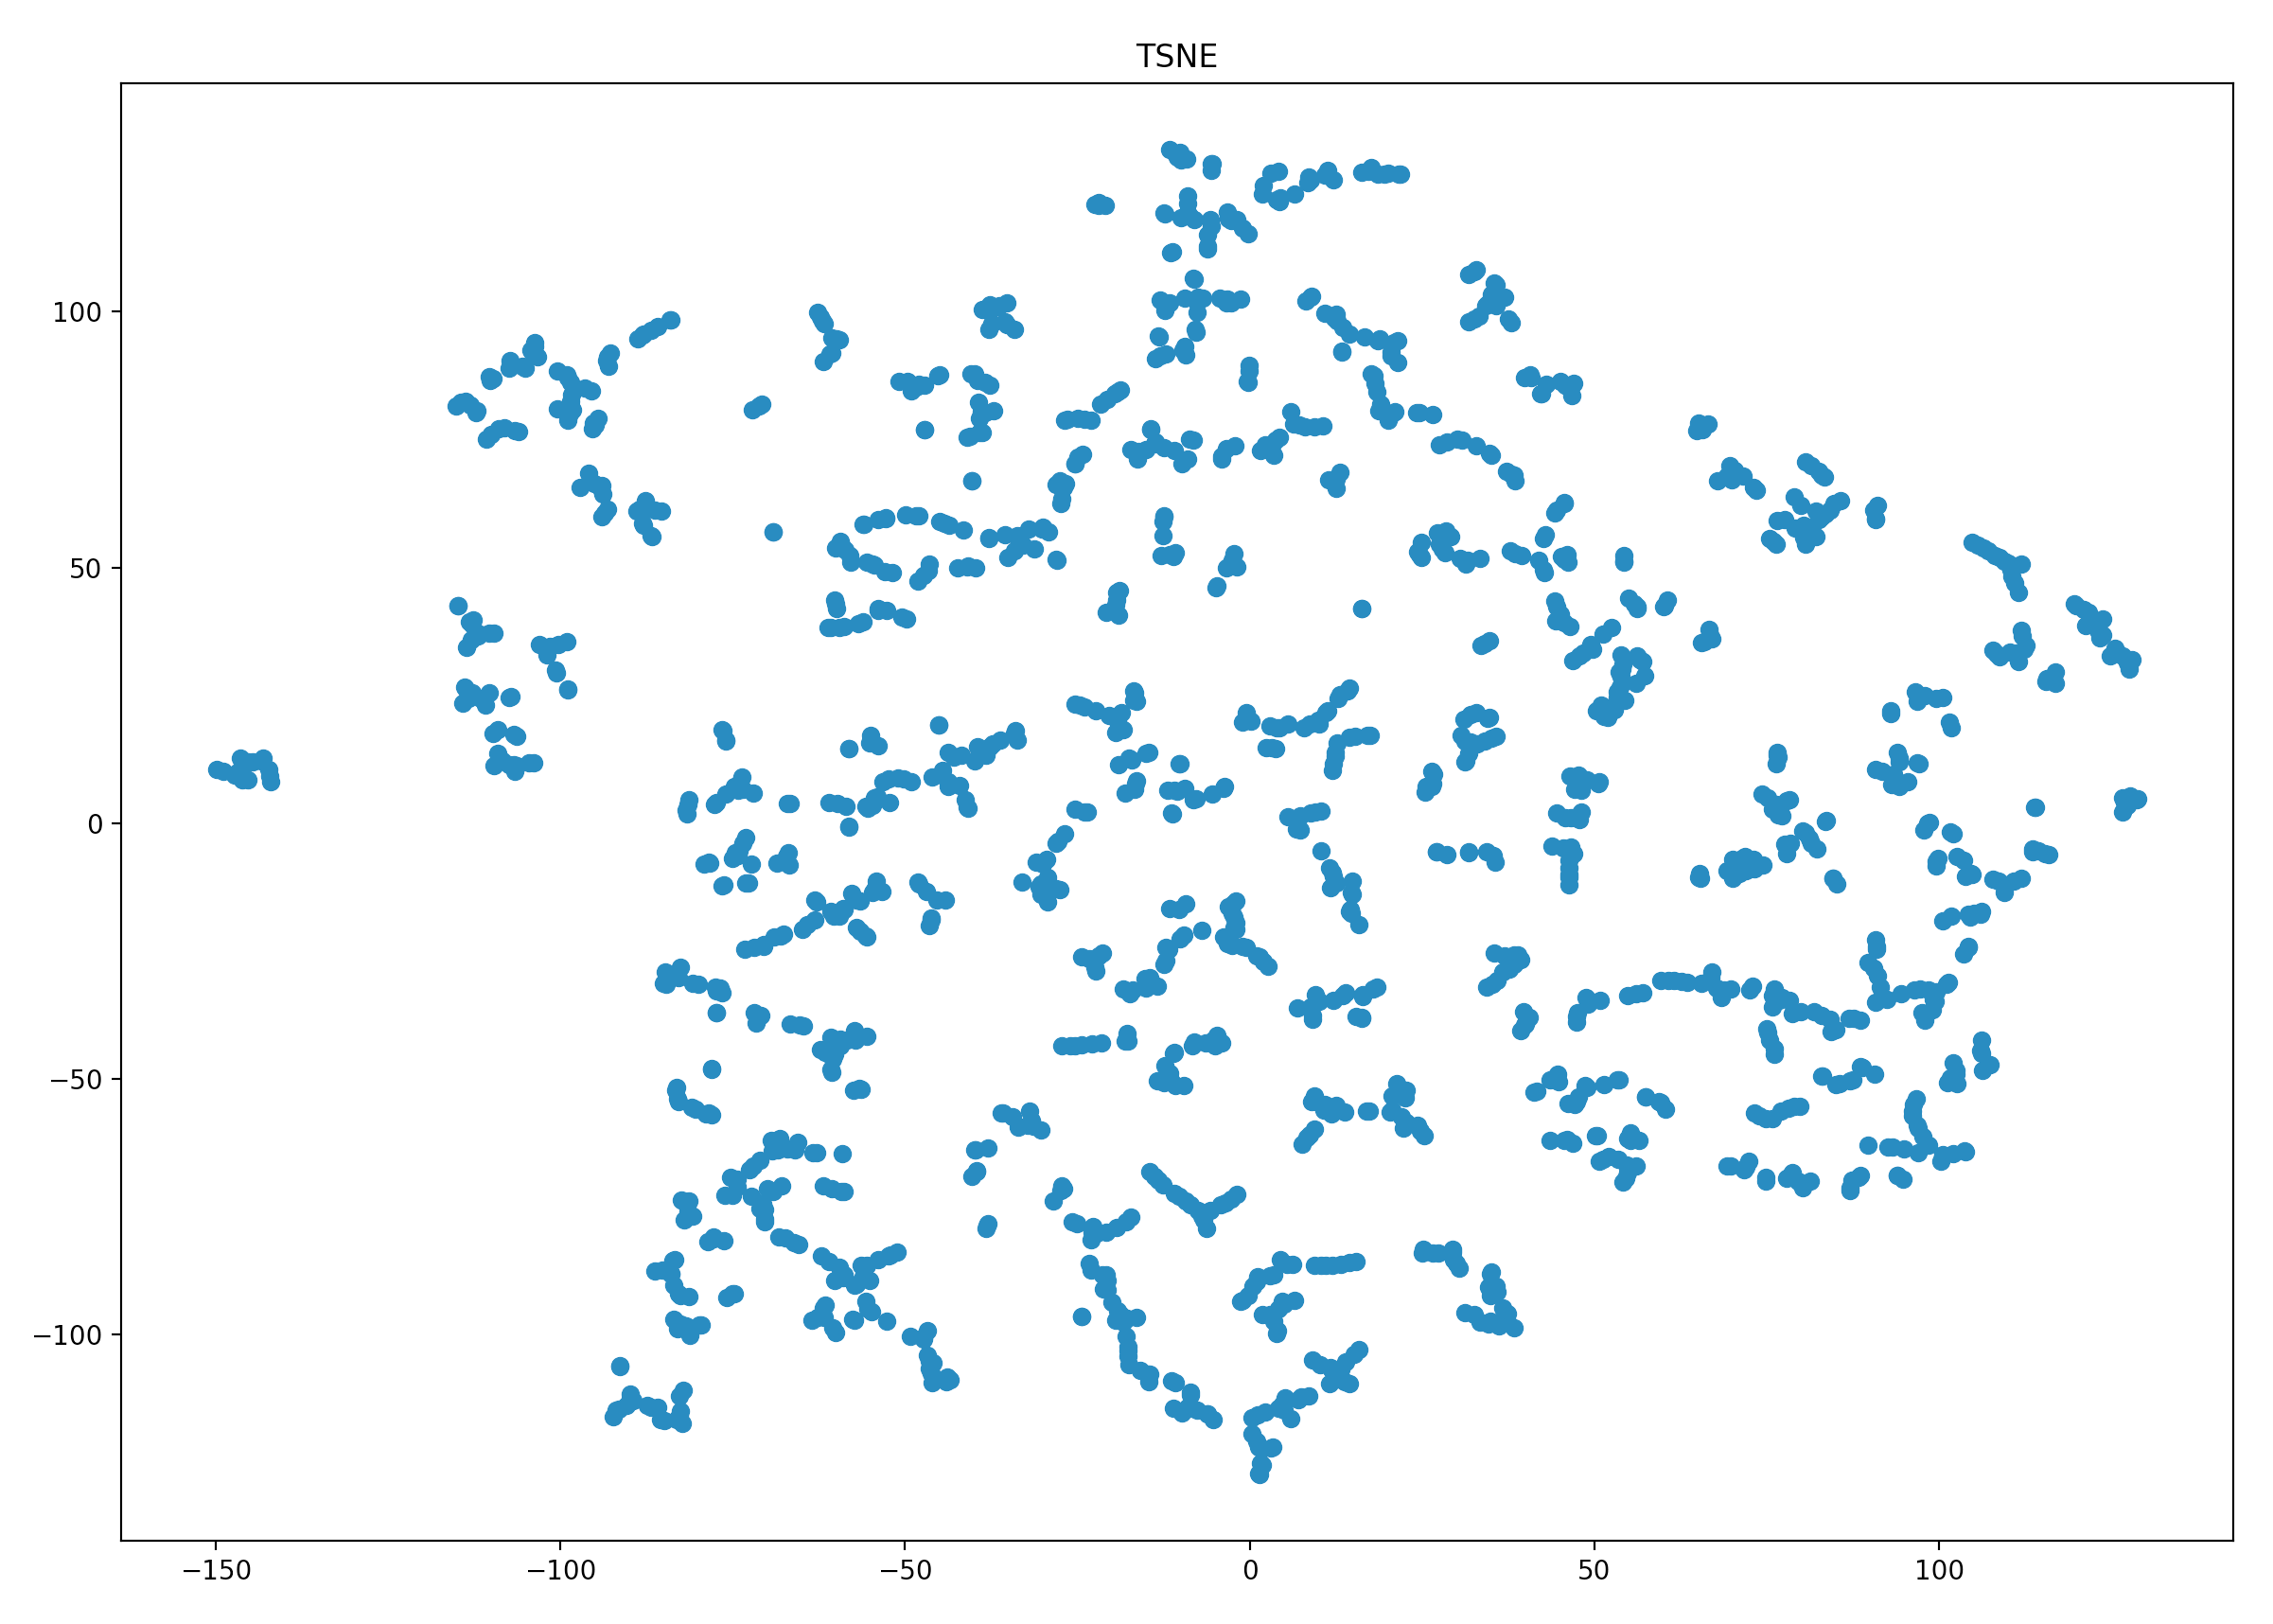
\includegraphics[width=0.9\textwidth]{./images/tsneParametersTest/perplexity/perp5-1hTSNE.png}
  % \caption{}
  % \label{figure:}
  \end{subfigure}%
  \begin{subfigure}{.5\textwidth}
    \centering
    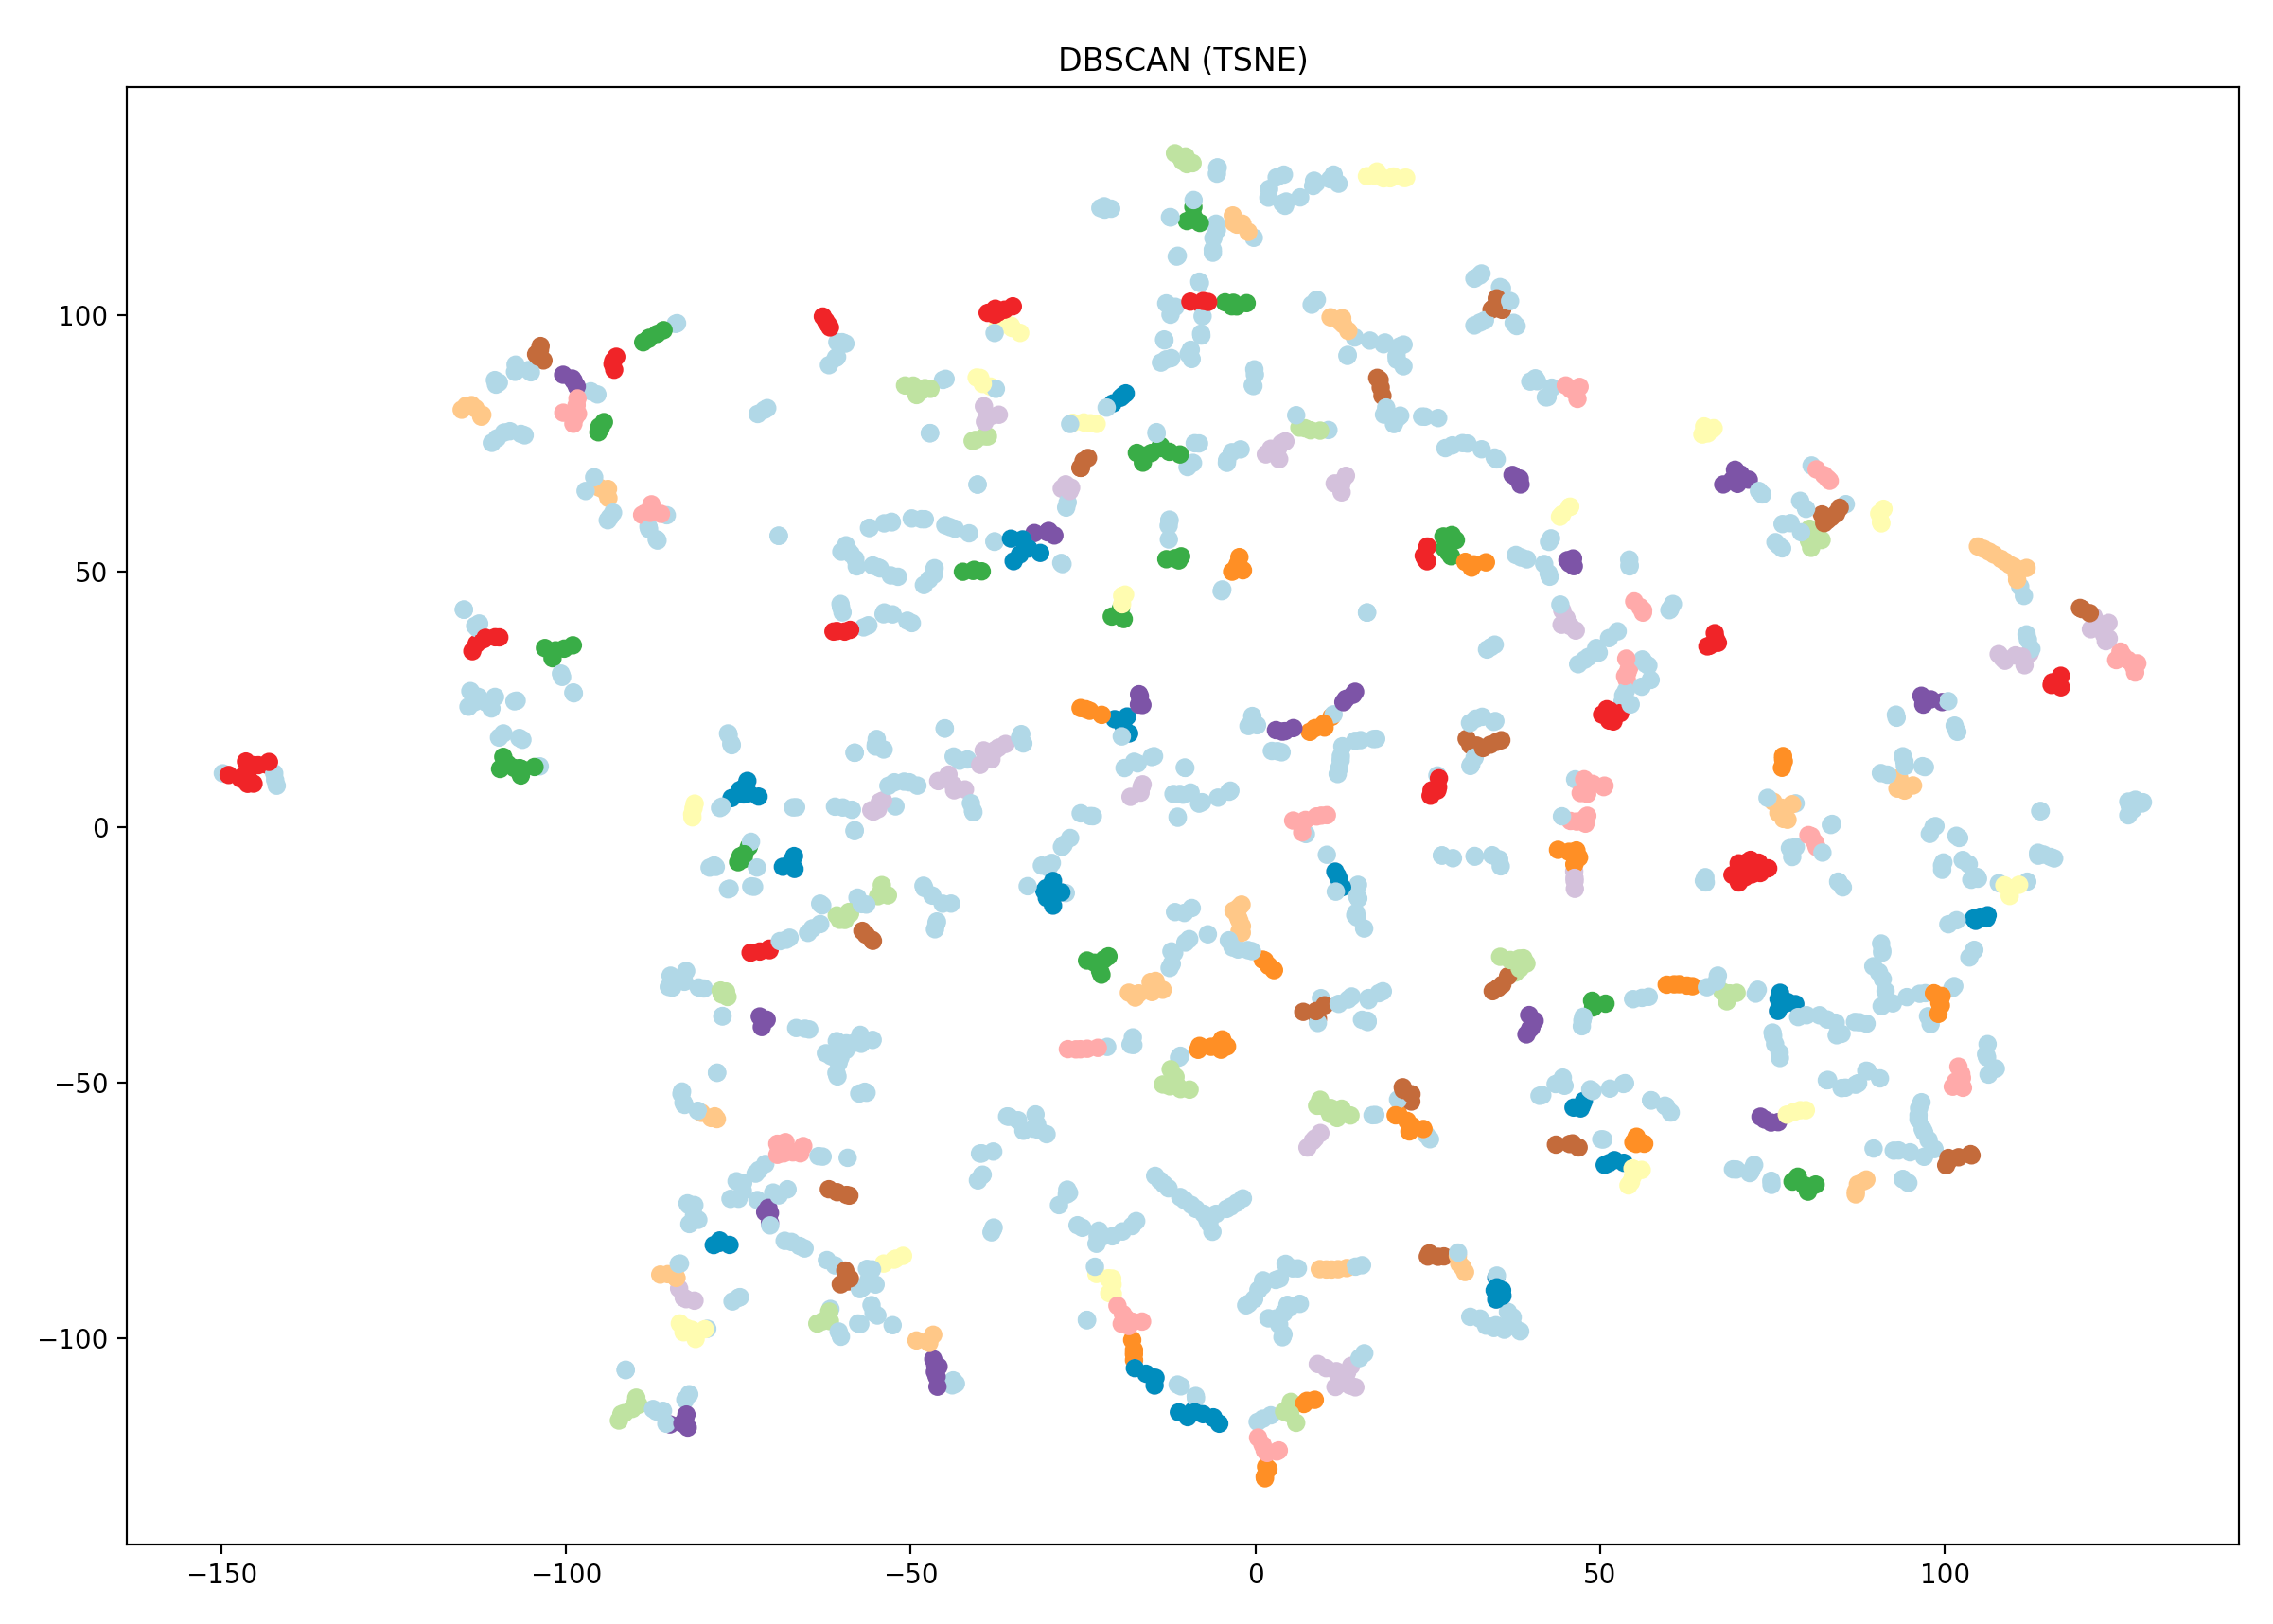
\includegraphics[width=0.9\textwidth]{./images/tsneParametersTest/perplexity/perp5-1hDBSCAN.png}
    % \caption{}
    % \label{figure:}
  \end{subfigure}
	\caption{\textbf{1h} data files, t-SNE calculated with the following parameters: \textbf{perplexity=5}, n\_iter=5000, learning\_rate=50}
	\label{figure:1hperp5TSNE}
\end{figure}


% -- 3h, perp 5 --
\begin{figure}[H]
	\centering
	
  \centering
	\begin{subfigure}{.5\textwidth}
    \centering
    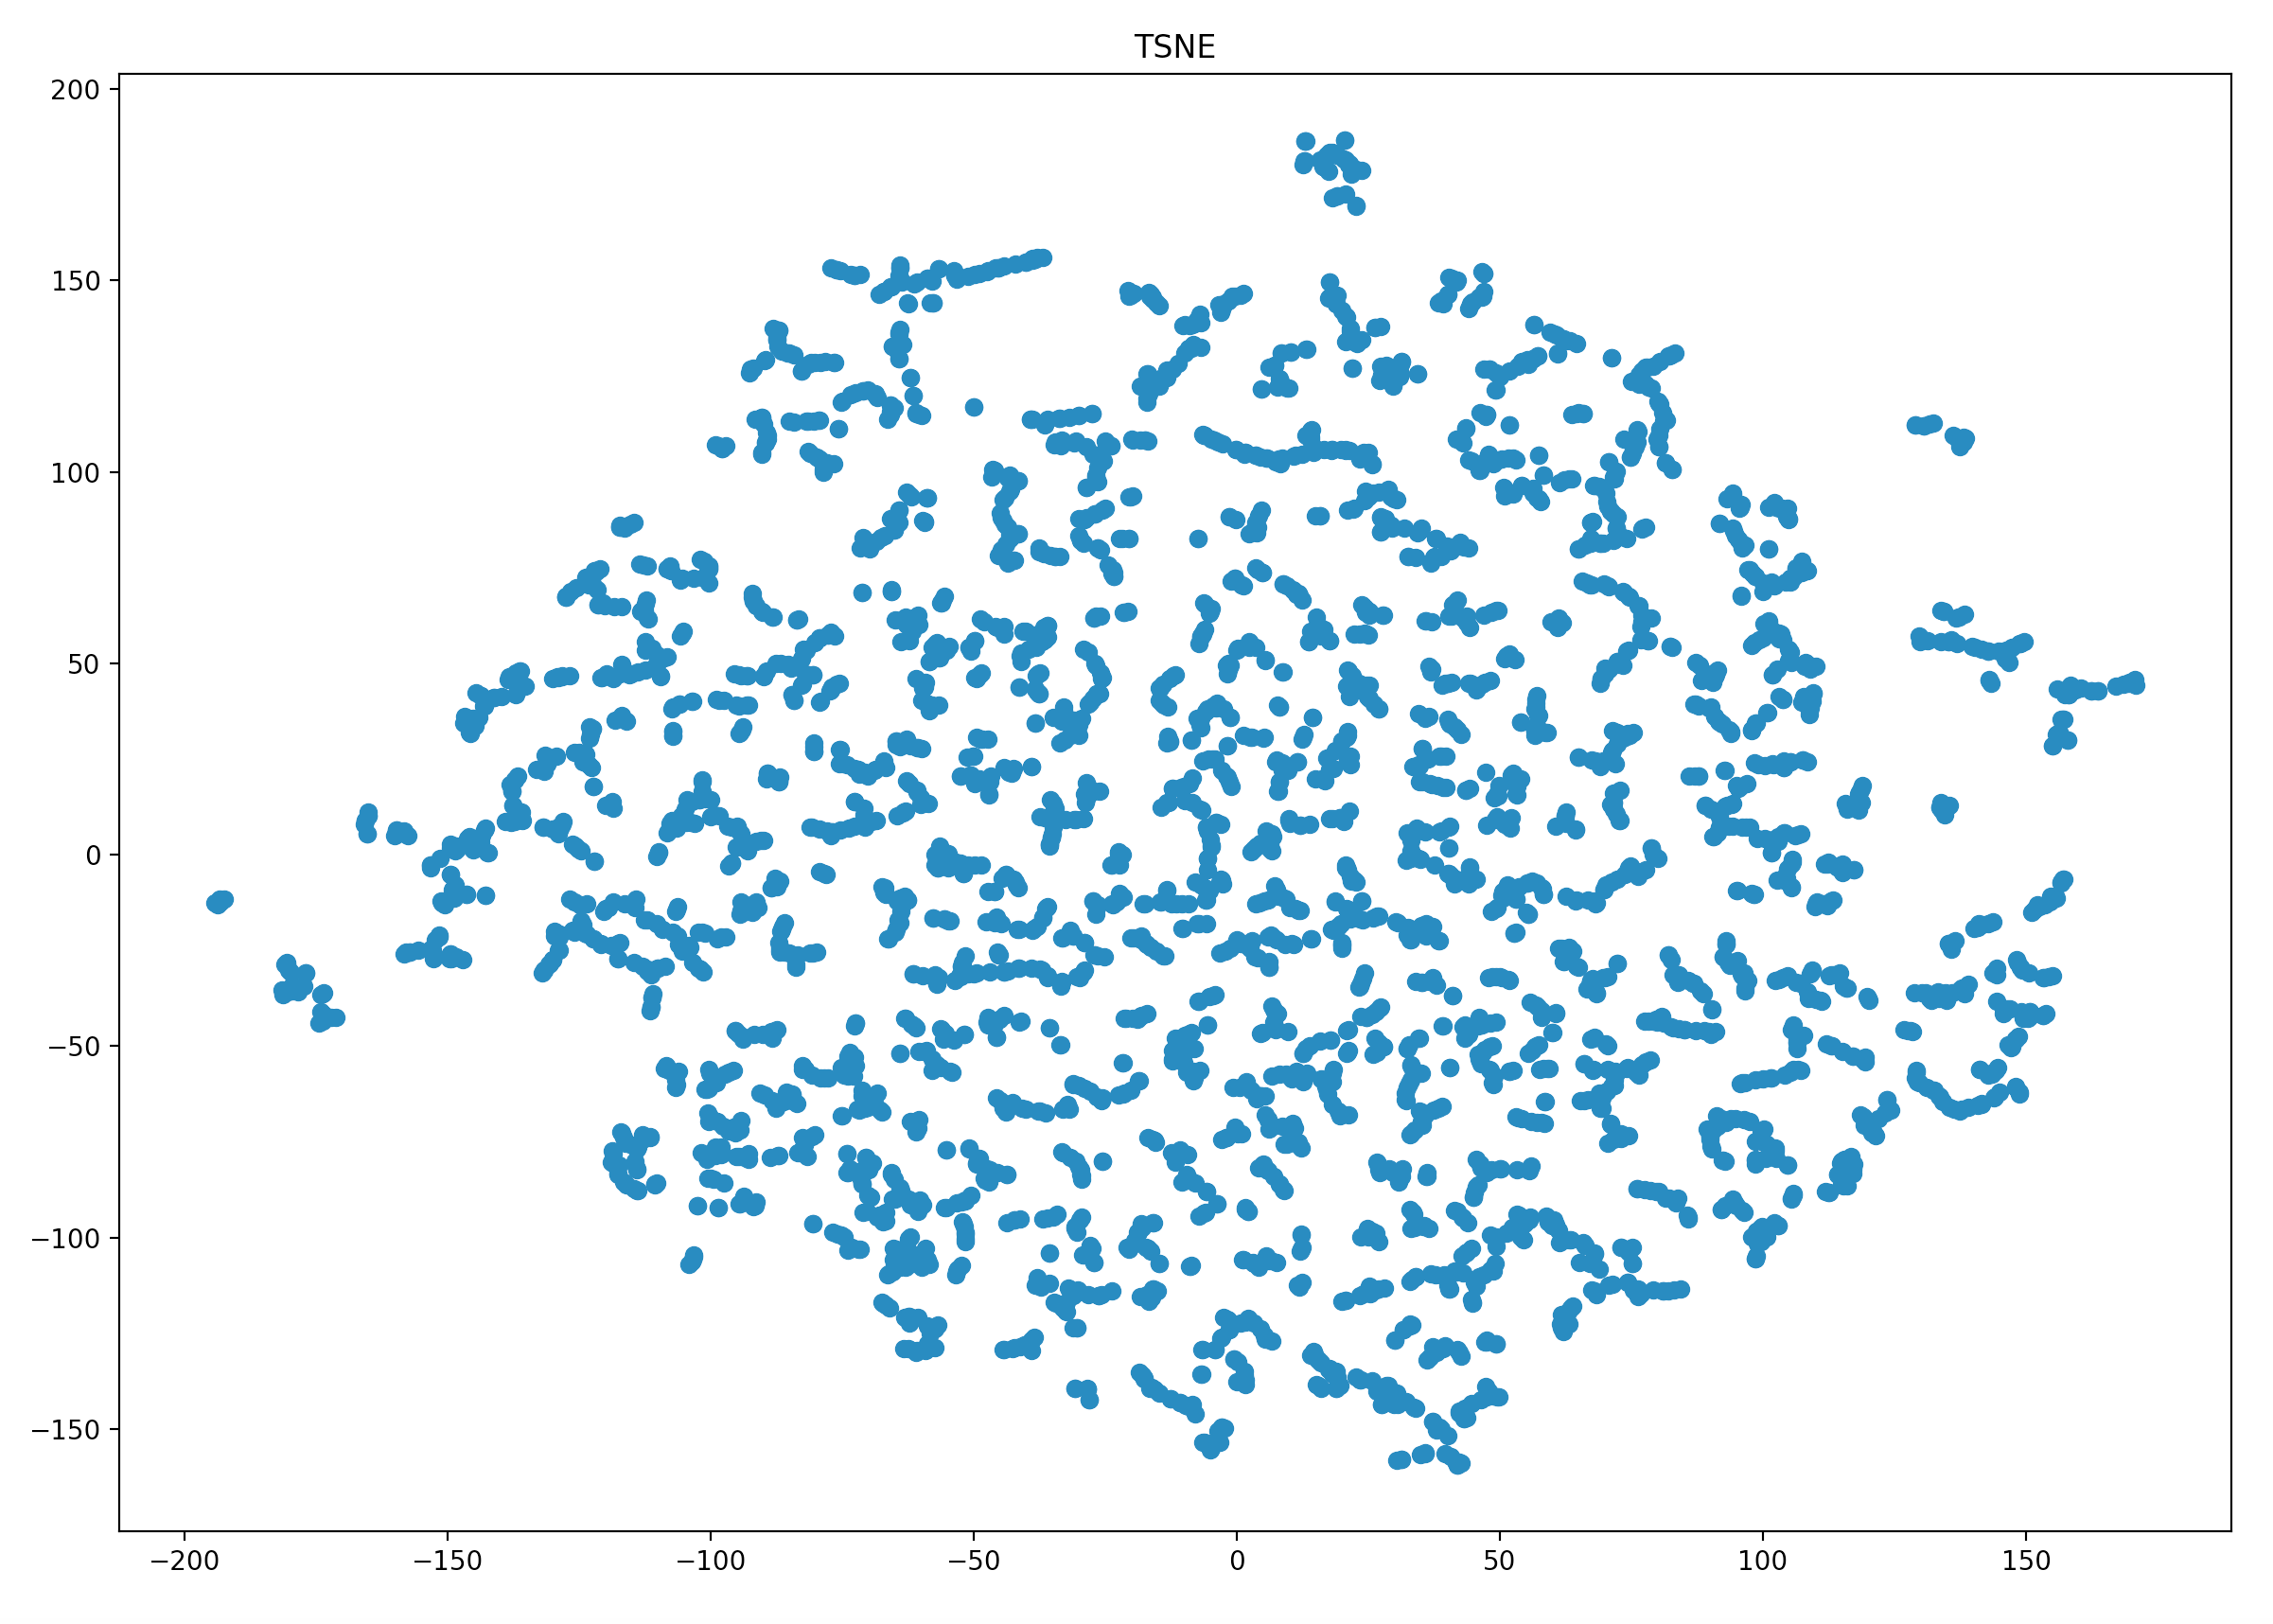
\includegraphics[width=0.9\textwidth]{./images/tsneParametersTest/perplexity/perp5-3hTSNE.png}
  % \caption{}
  % \label{figure:}
  \end{subfigure}%
  \begin{subfigure}{.5\textwidth}
    \centering
    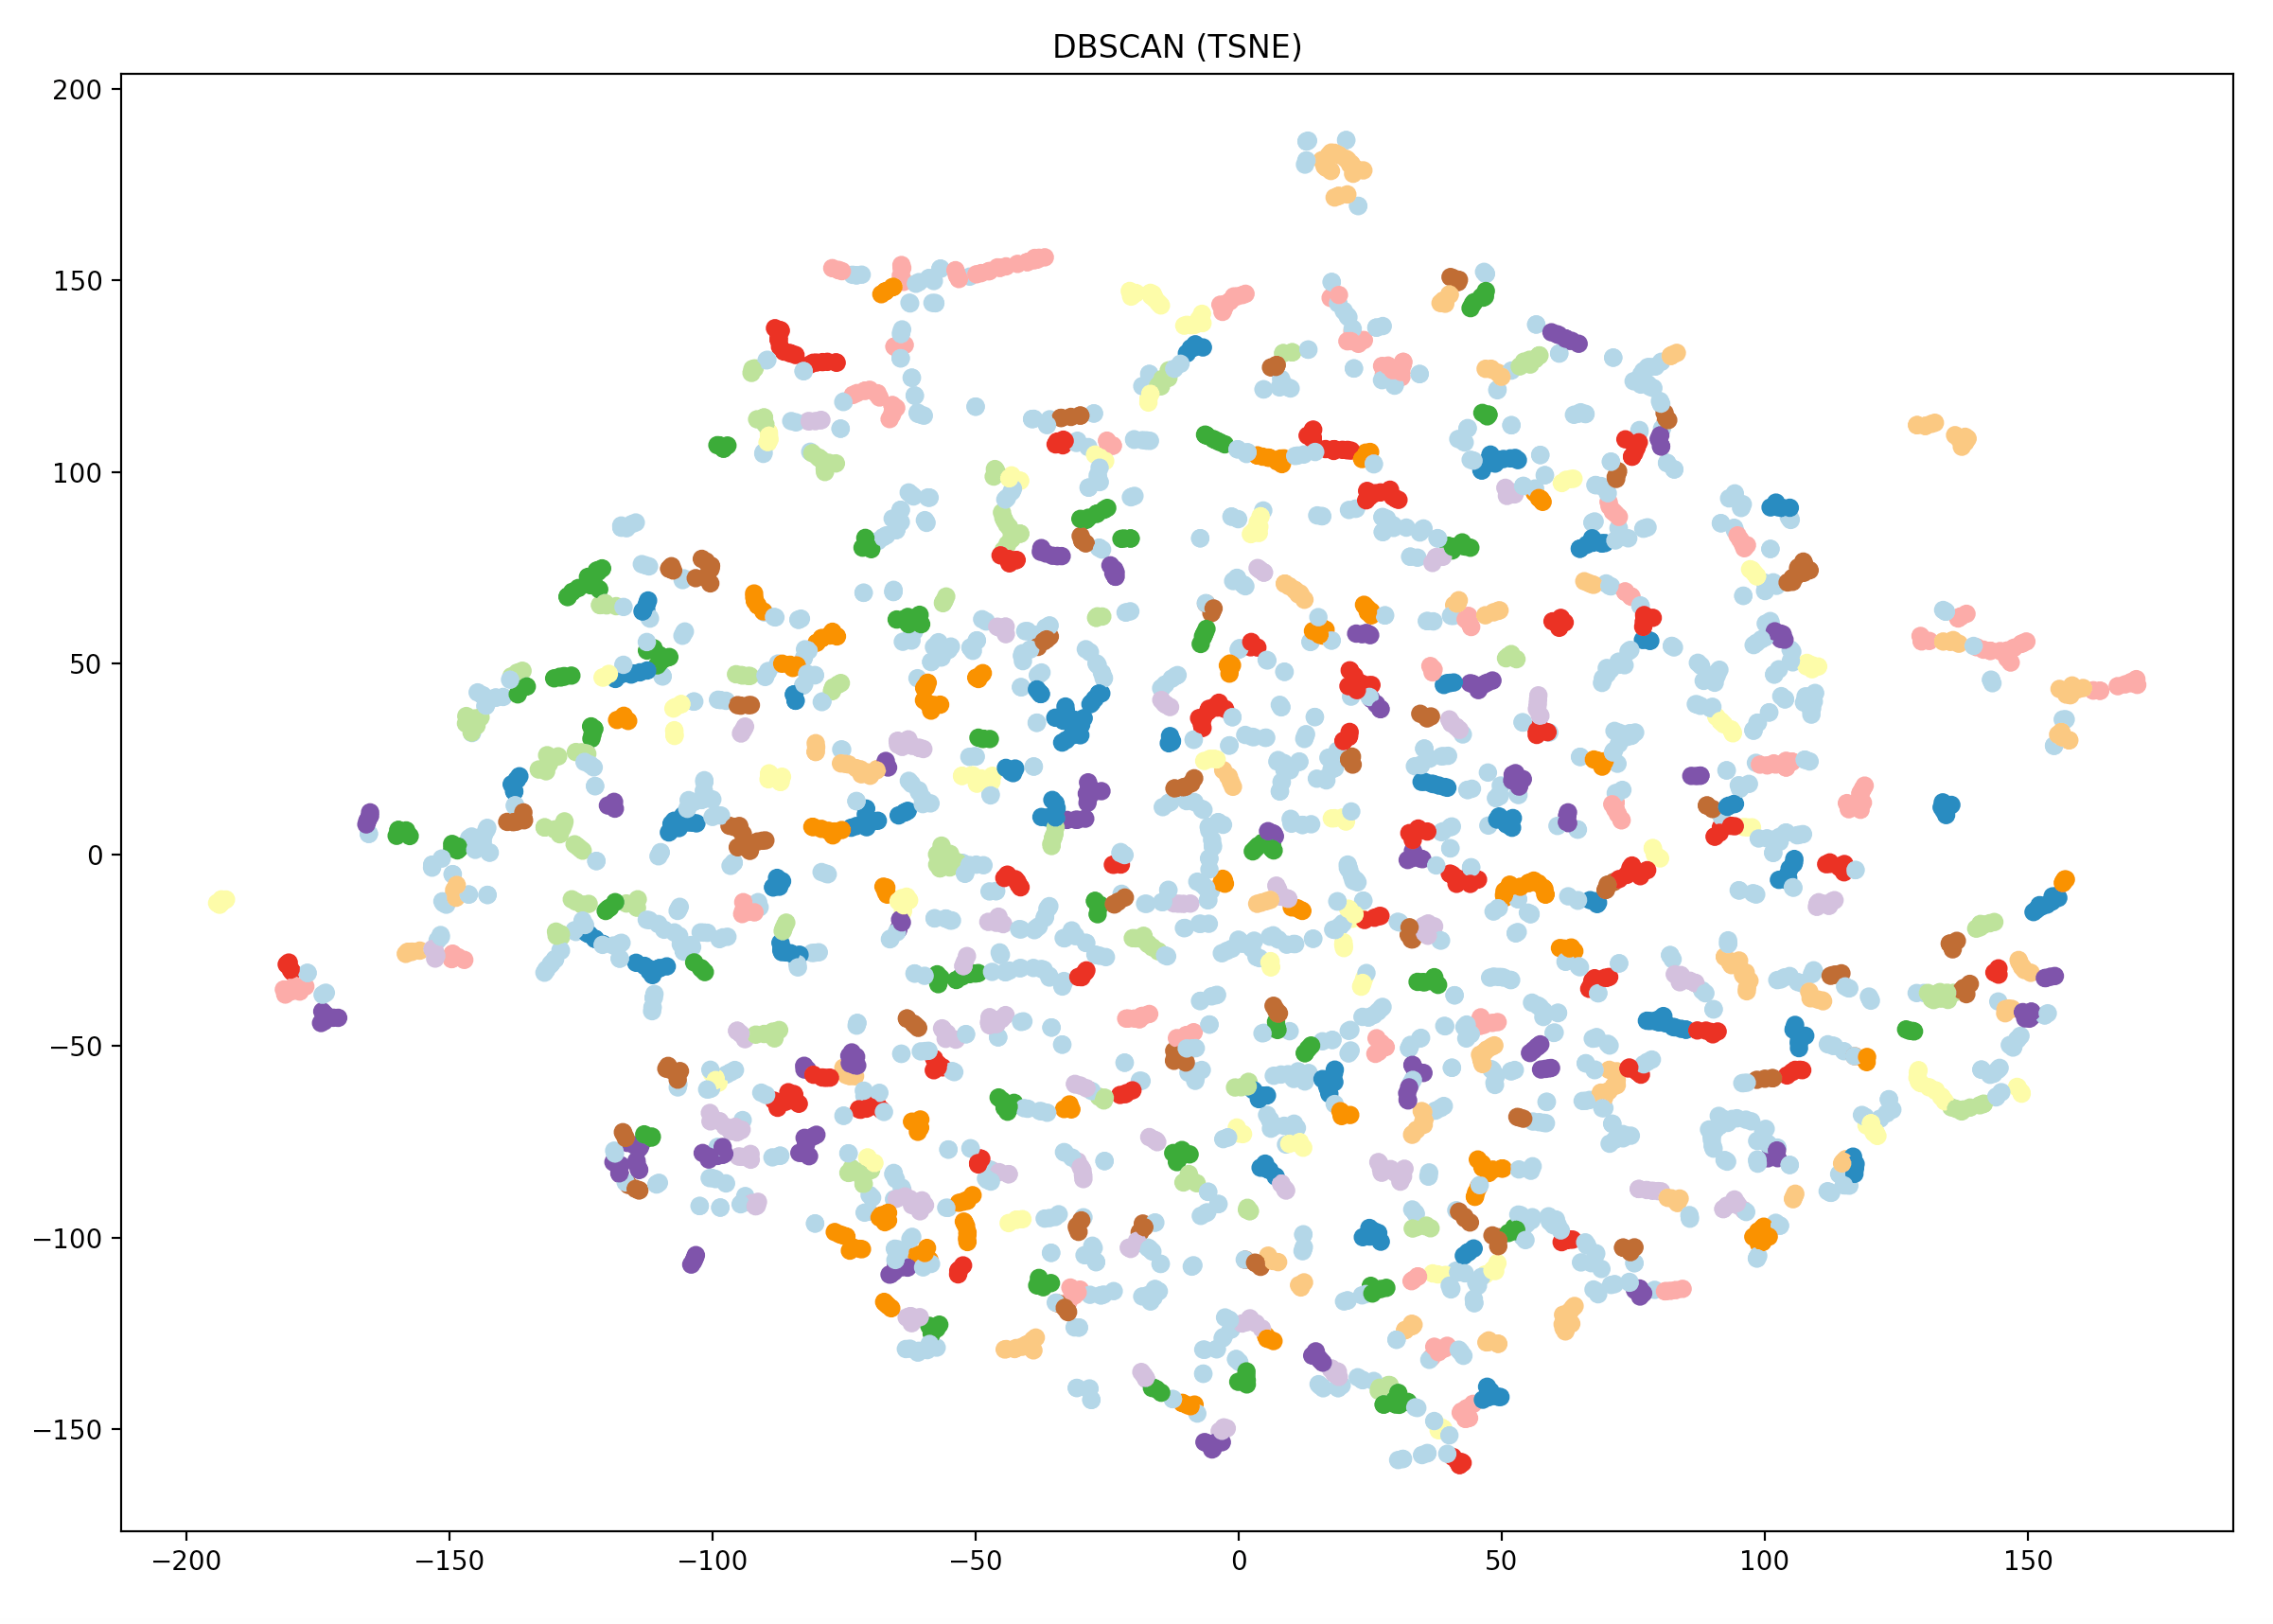
\includegraphics[width=0.9\textwidth]{./images/tsneParametersTest/perplexity/perp5-3hDBSCAN.png}
    % \caption{}
    % \label{figure:}
	\end{subfigure}
	\caption{\textbf{3h} data files, t-SNE calculated with the following parameters: \textbf{perplexity=5}, n\_iter=5000, learning\_rate=50}
  \label{figure:3hperp5TSNE}
\end{figure}


%------------------ PERPLEXITY 10: ------------------
\subsubsection{Perplexity = 10}
% -- 1h, perp 10 --
\begin{figure}[H]
  \centering
  \begin{subfigure}{.5\textwidth}
    \centering
    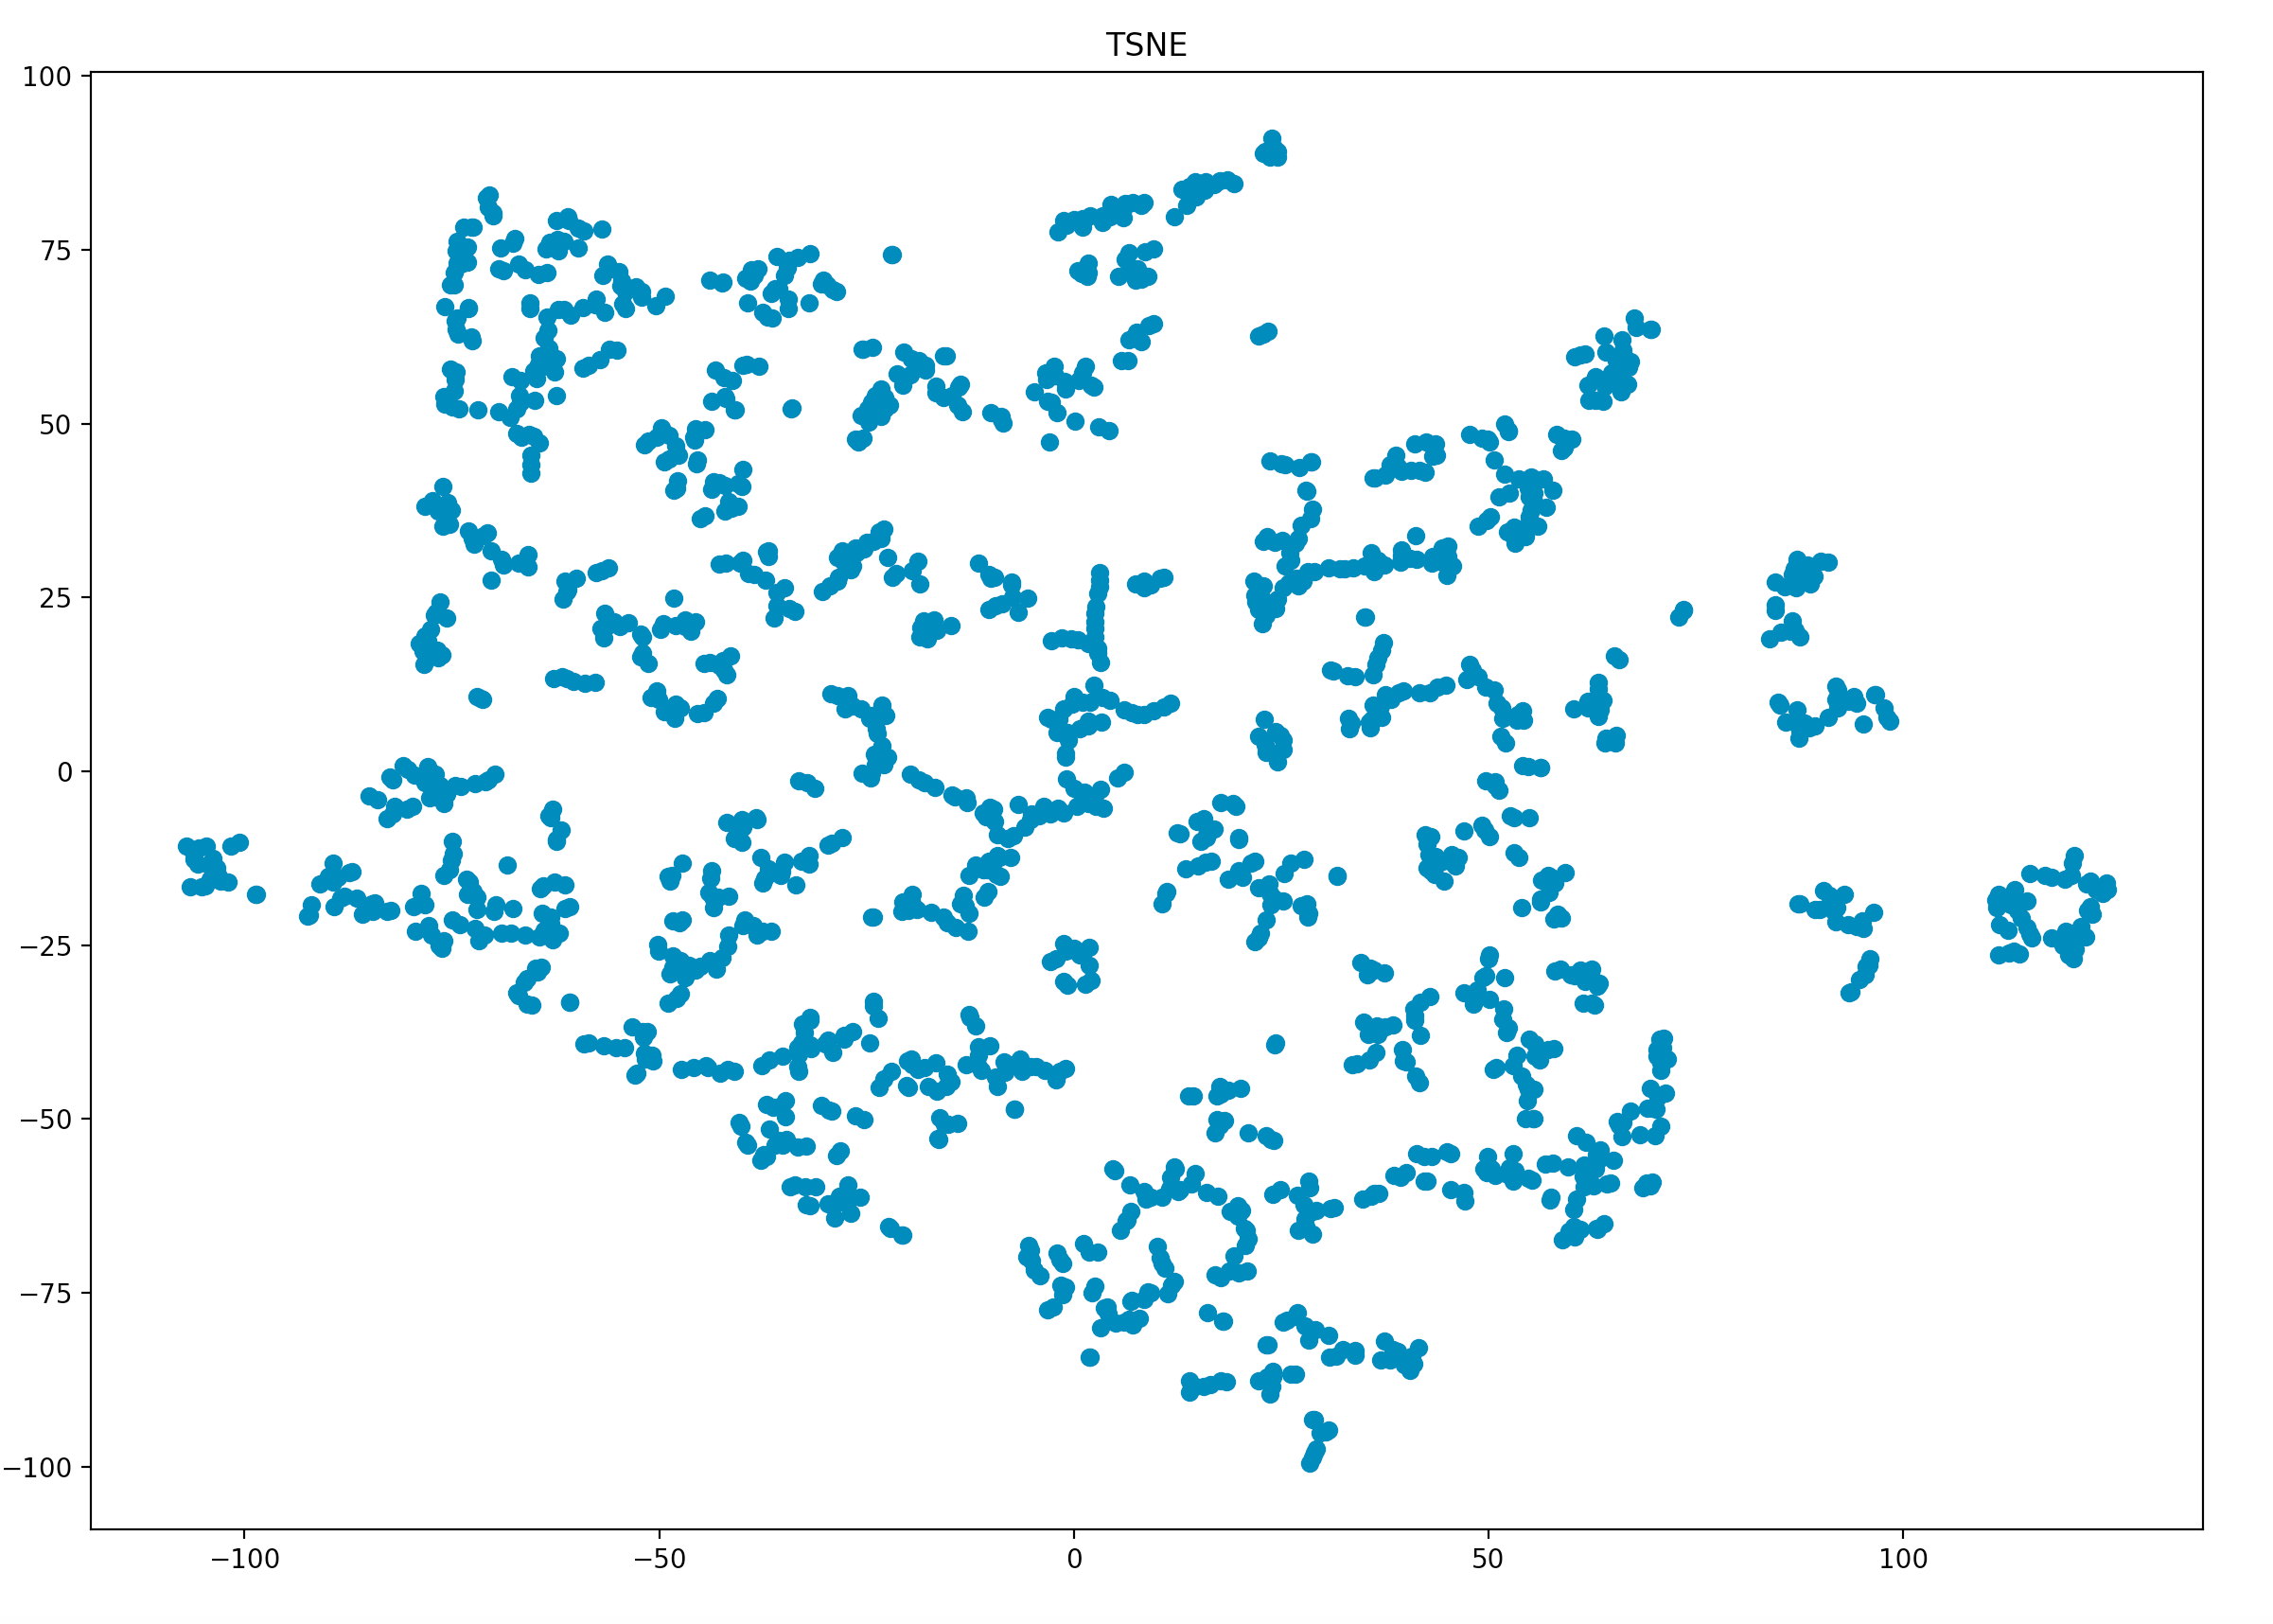
\includegraphics[width=0.9\textwidth]{./images/tsneParametersTest/perplexity/perp10-1hTSNE.png}
  % \caption{}
  % \label{figure:}
  \end{subfigure}%
  \begin{subfigure}{.5\textwidth}
    \centering
    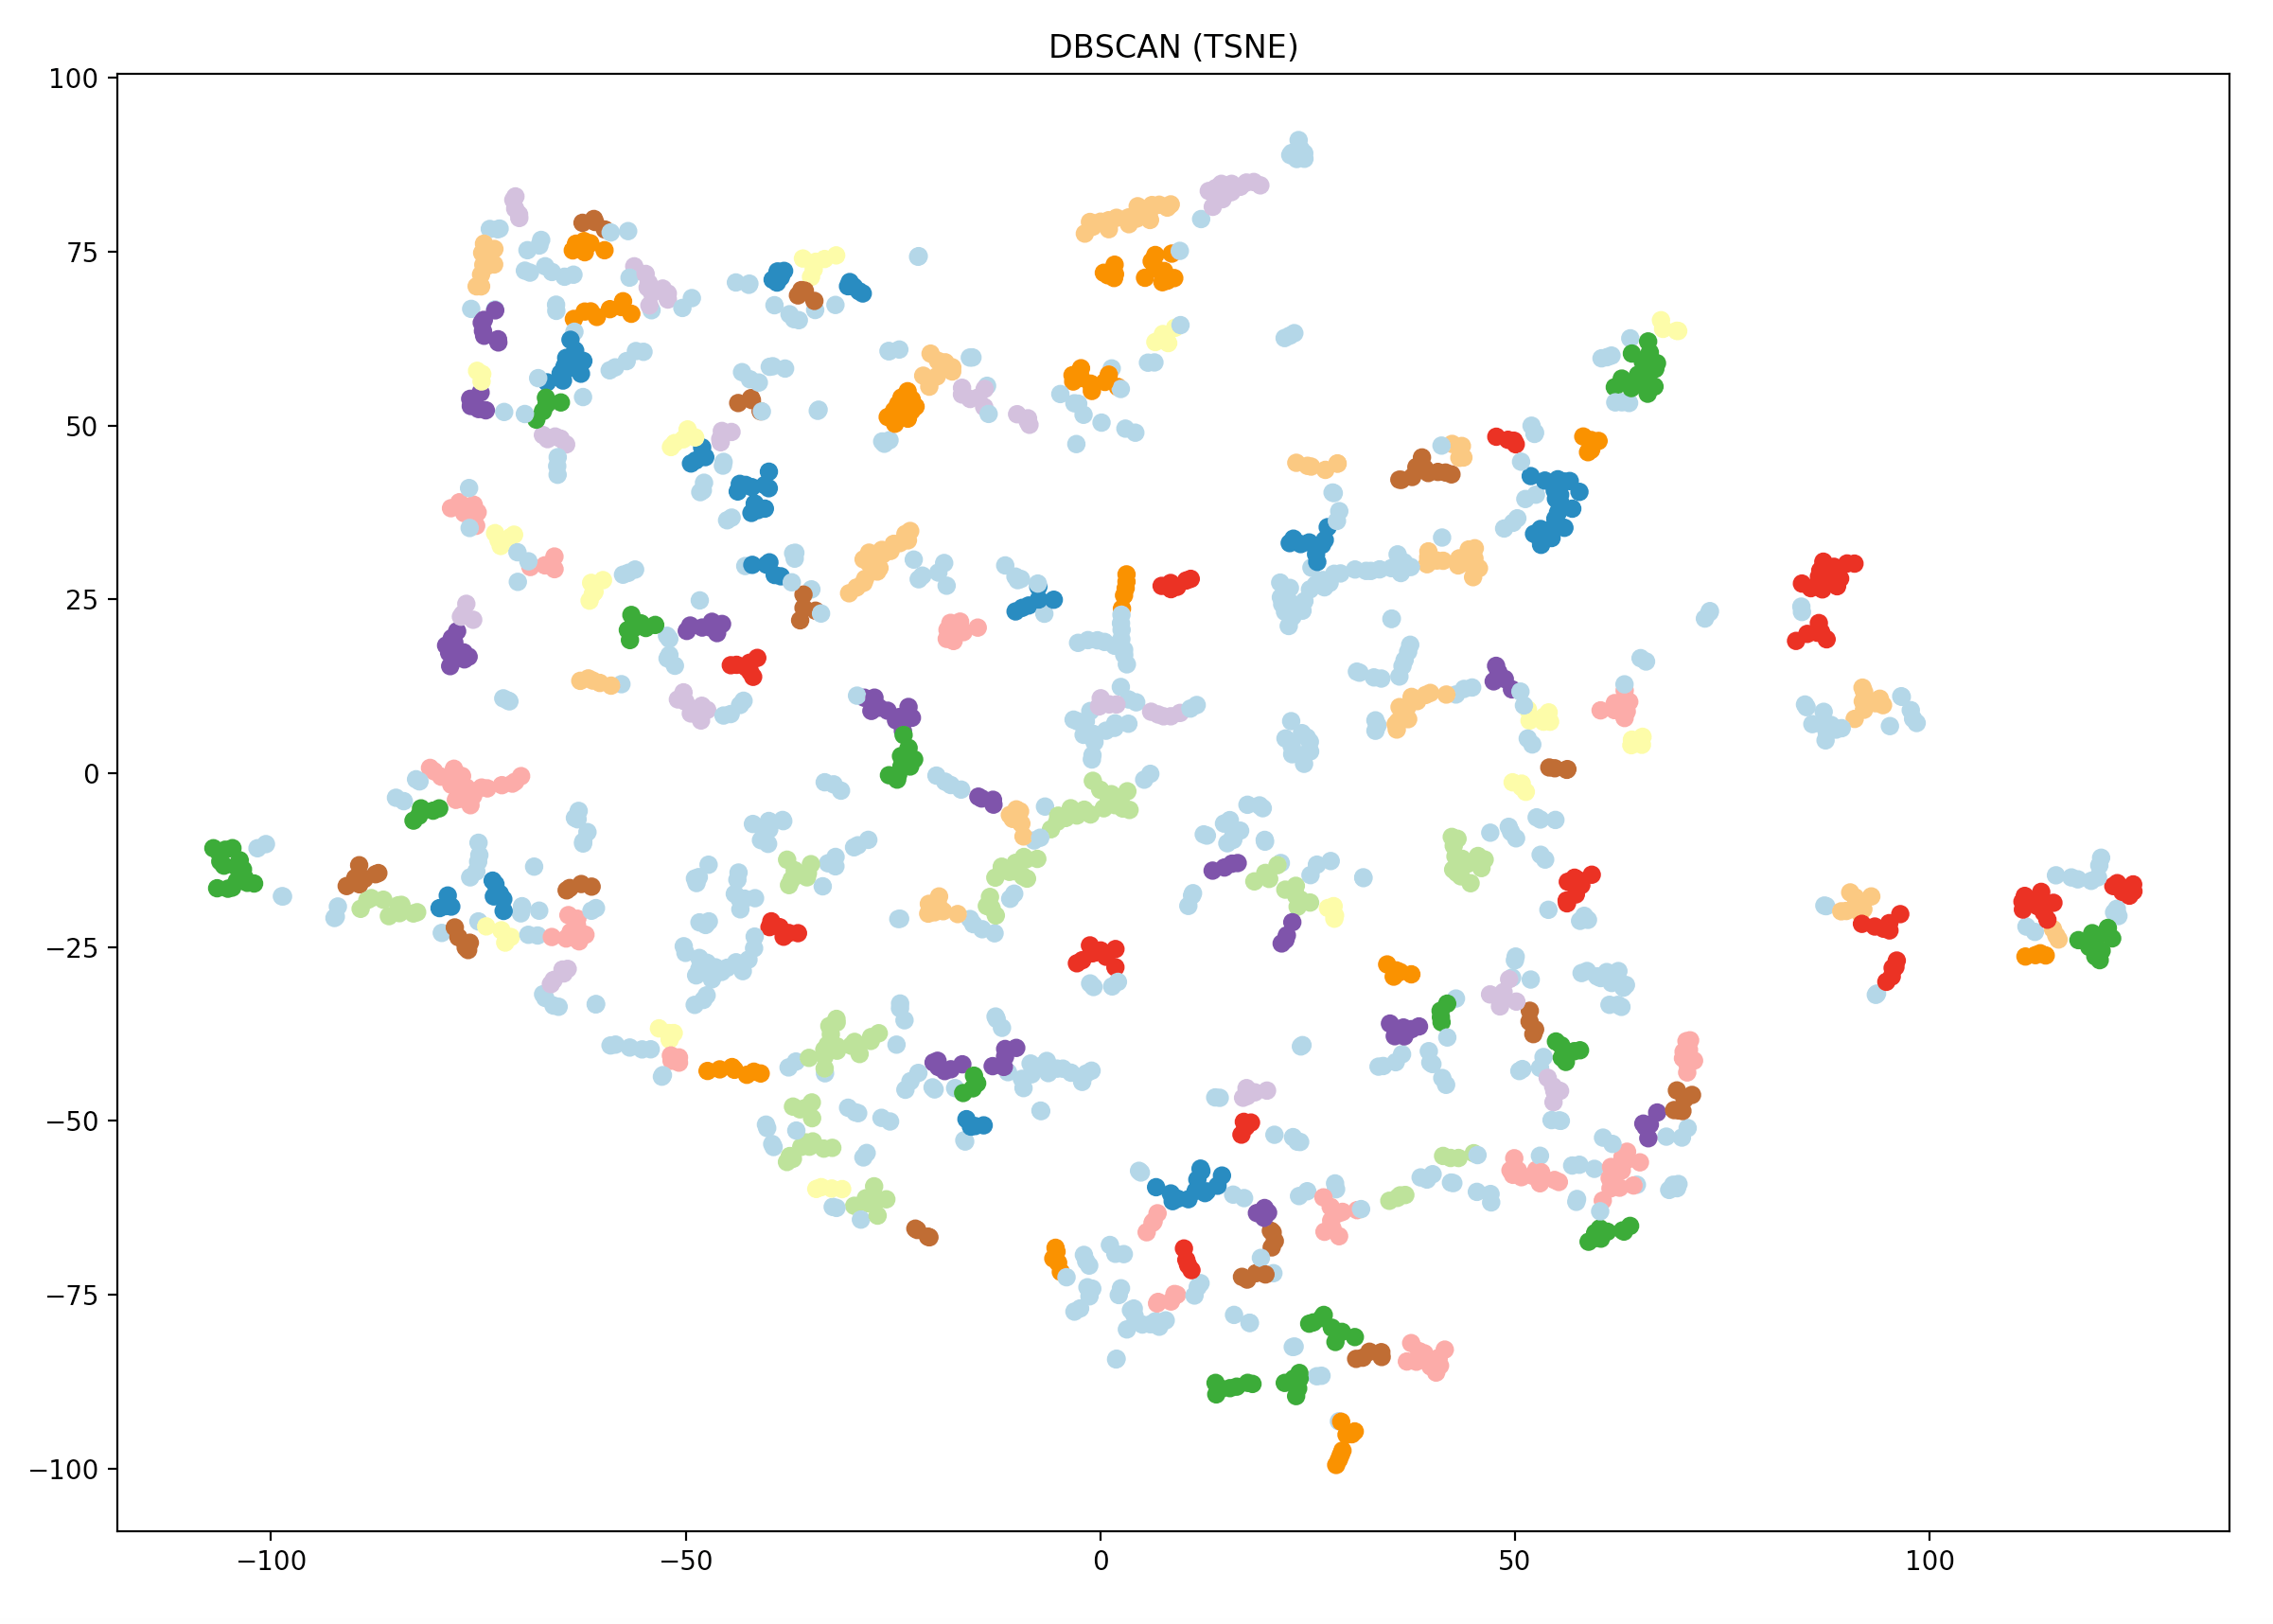
\includegraphics[width=0.9\textwidth]{./images/tsneParametersTest/perplexity/perp10-1hDBSCAN.png}
    % \caption{}
    % \label{figure:}
  \end{subfigure}
	\caption{\textbf{1h} data files, t-SNE calculated with the following parameters: \textbf{perplexity=10}, n\_iter=5000, learning\_rate=50}
  \label{figure:1hperp10TSNE}
\end{figure}

% -- 3h, perp 10 --
\begin{figure}[H]
  \centering
	\begin{subfigure}{.5\textwidth}
    \centering
    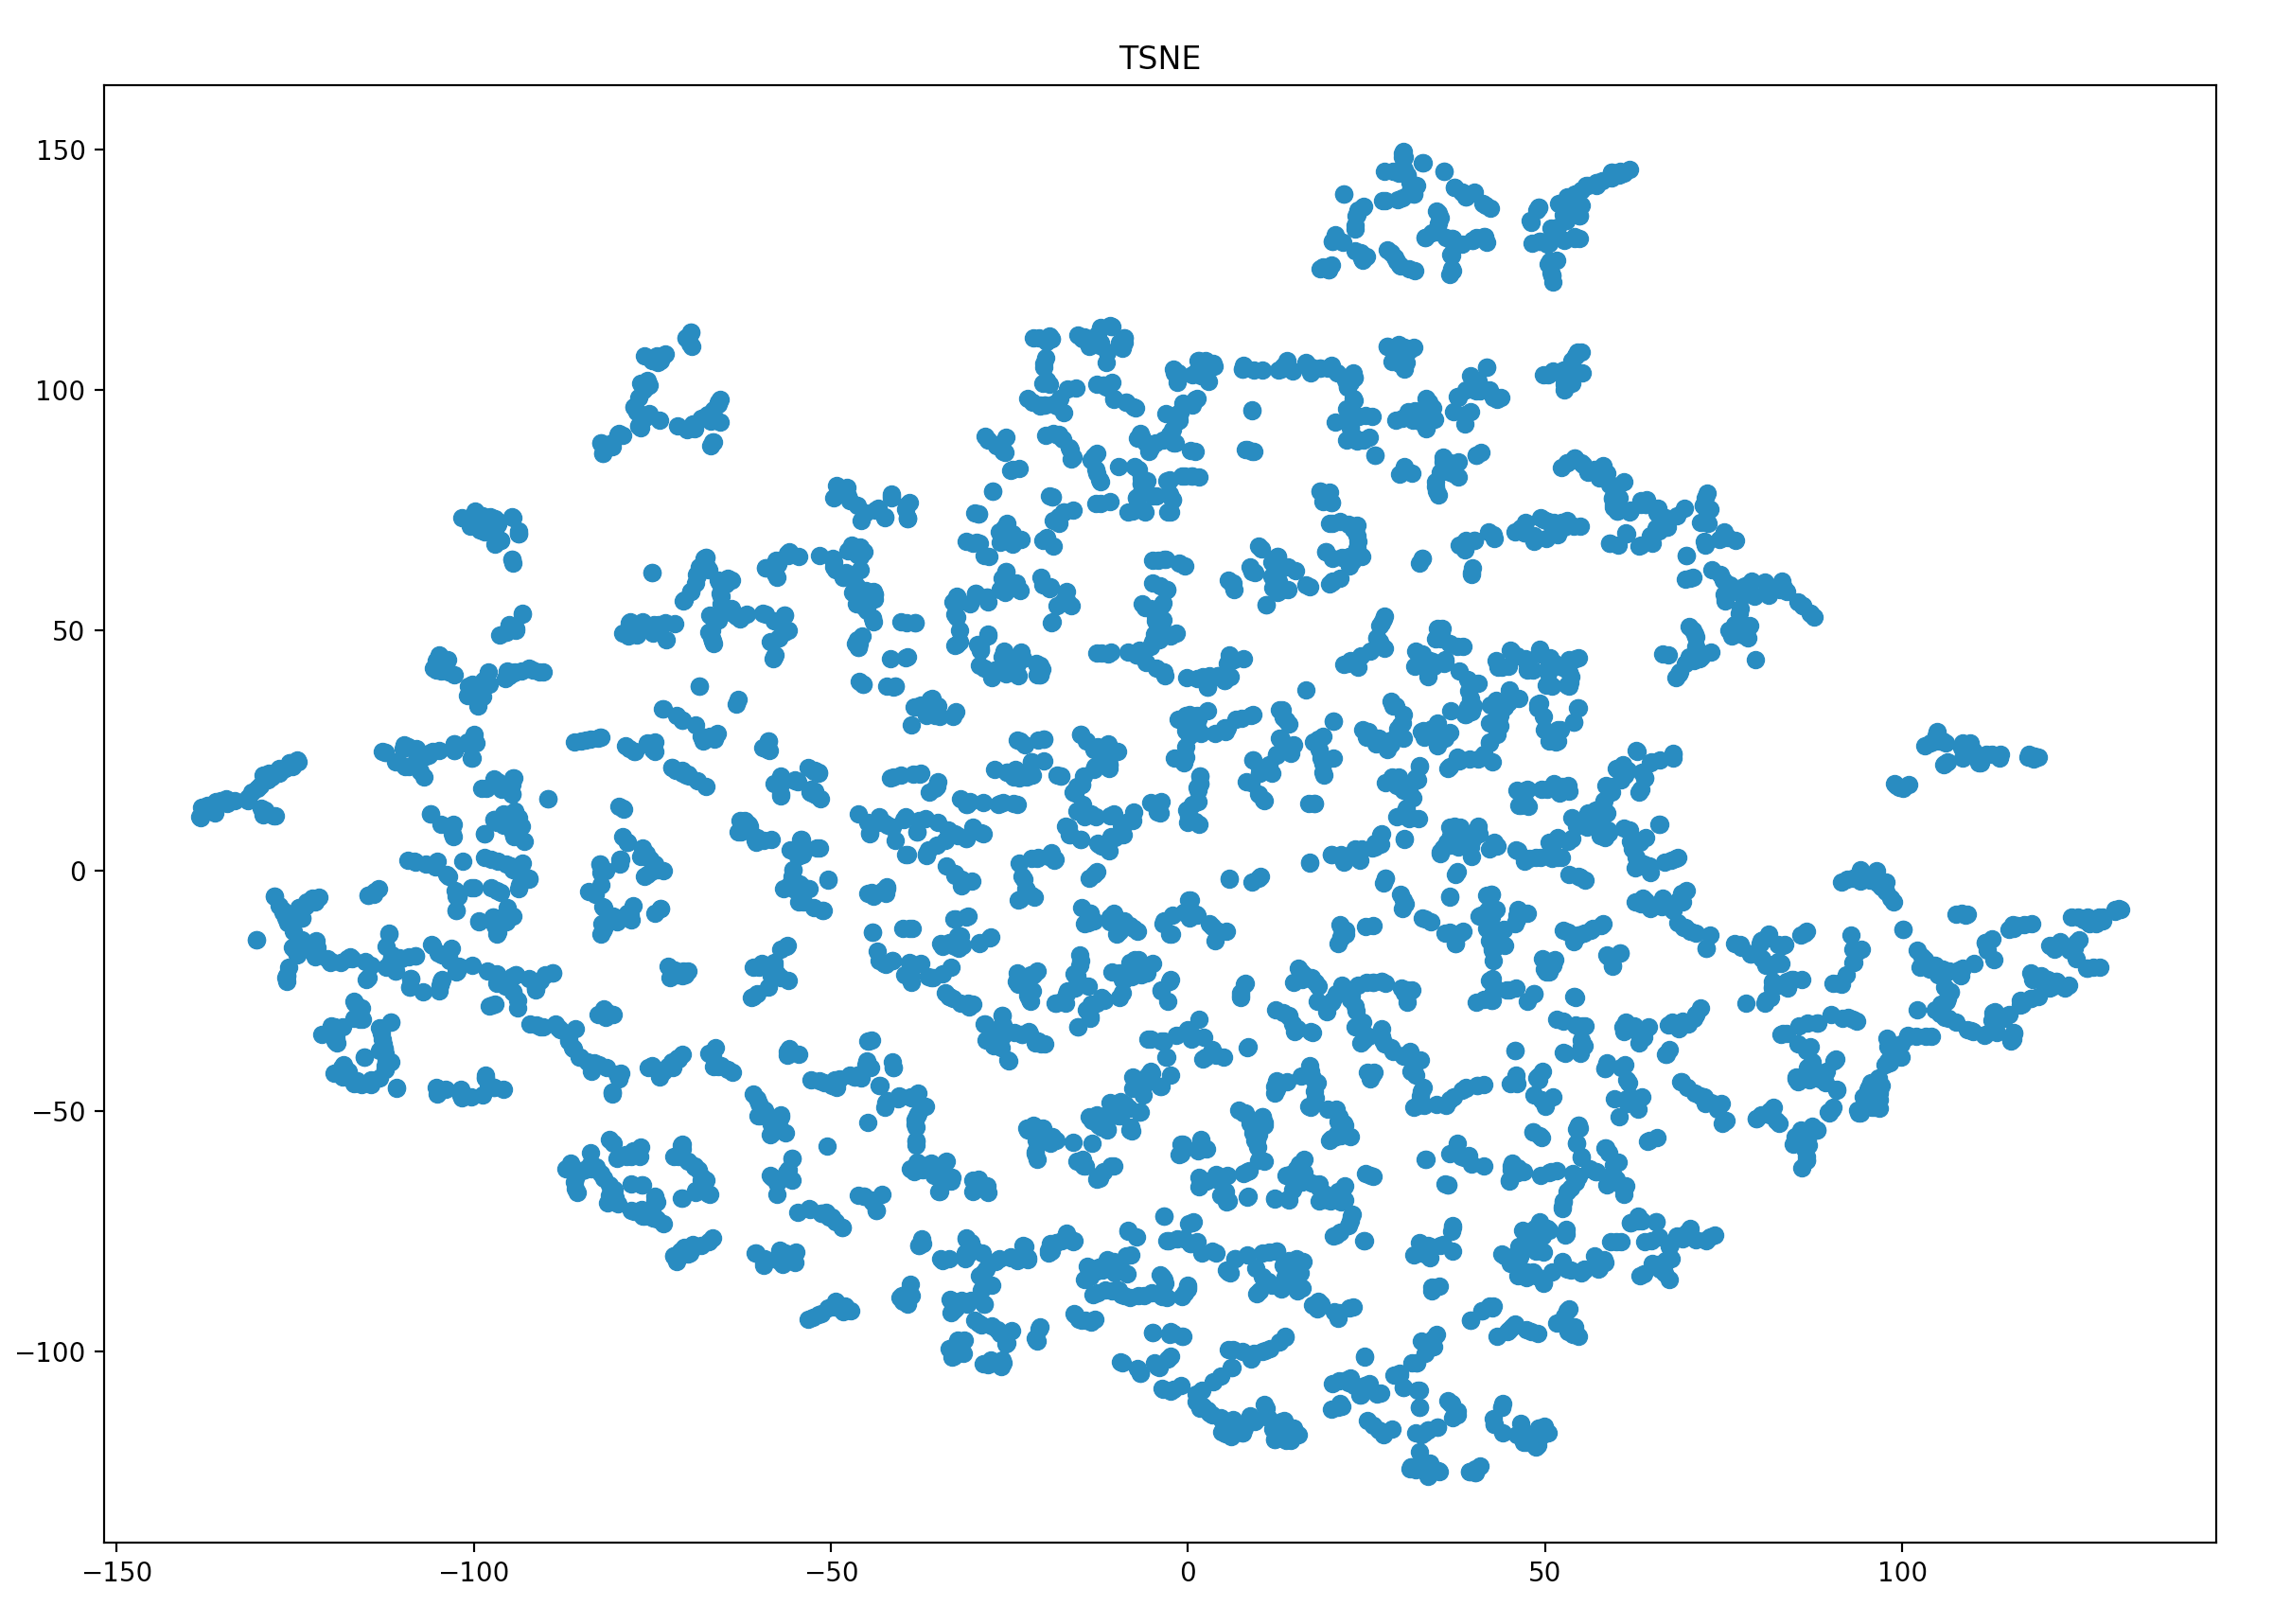
\includegraphics[width=0.9\textwidth]{./images/tsneParametersTest/perplexity/perp10-3hTSNE.png}
  % \caption{}
  % \label{figure:}
  \end{subfigure}%
  \begin{subfigure}{.5\textwidth}
    \centering
    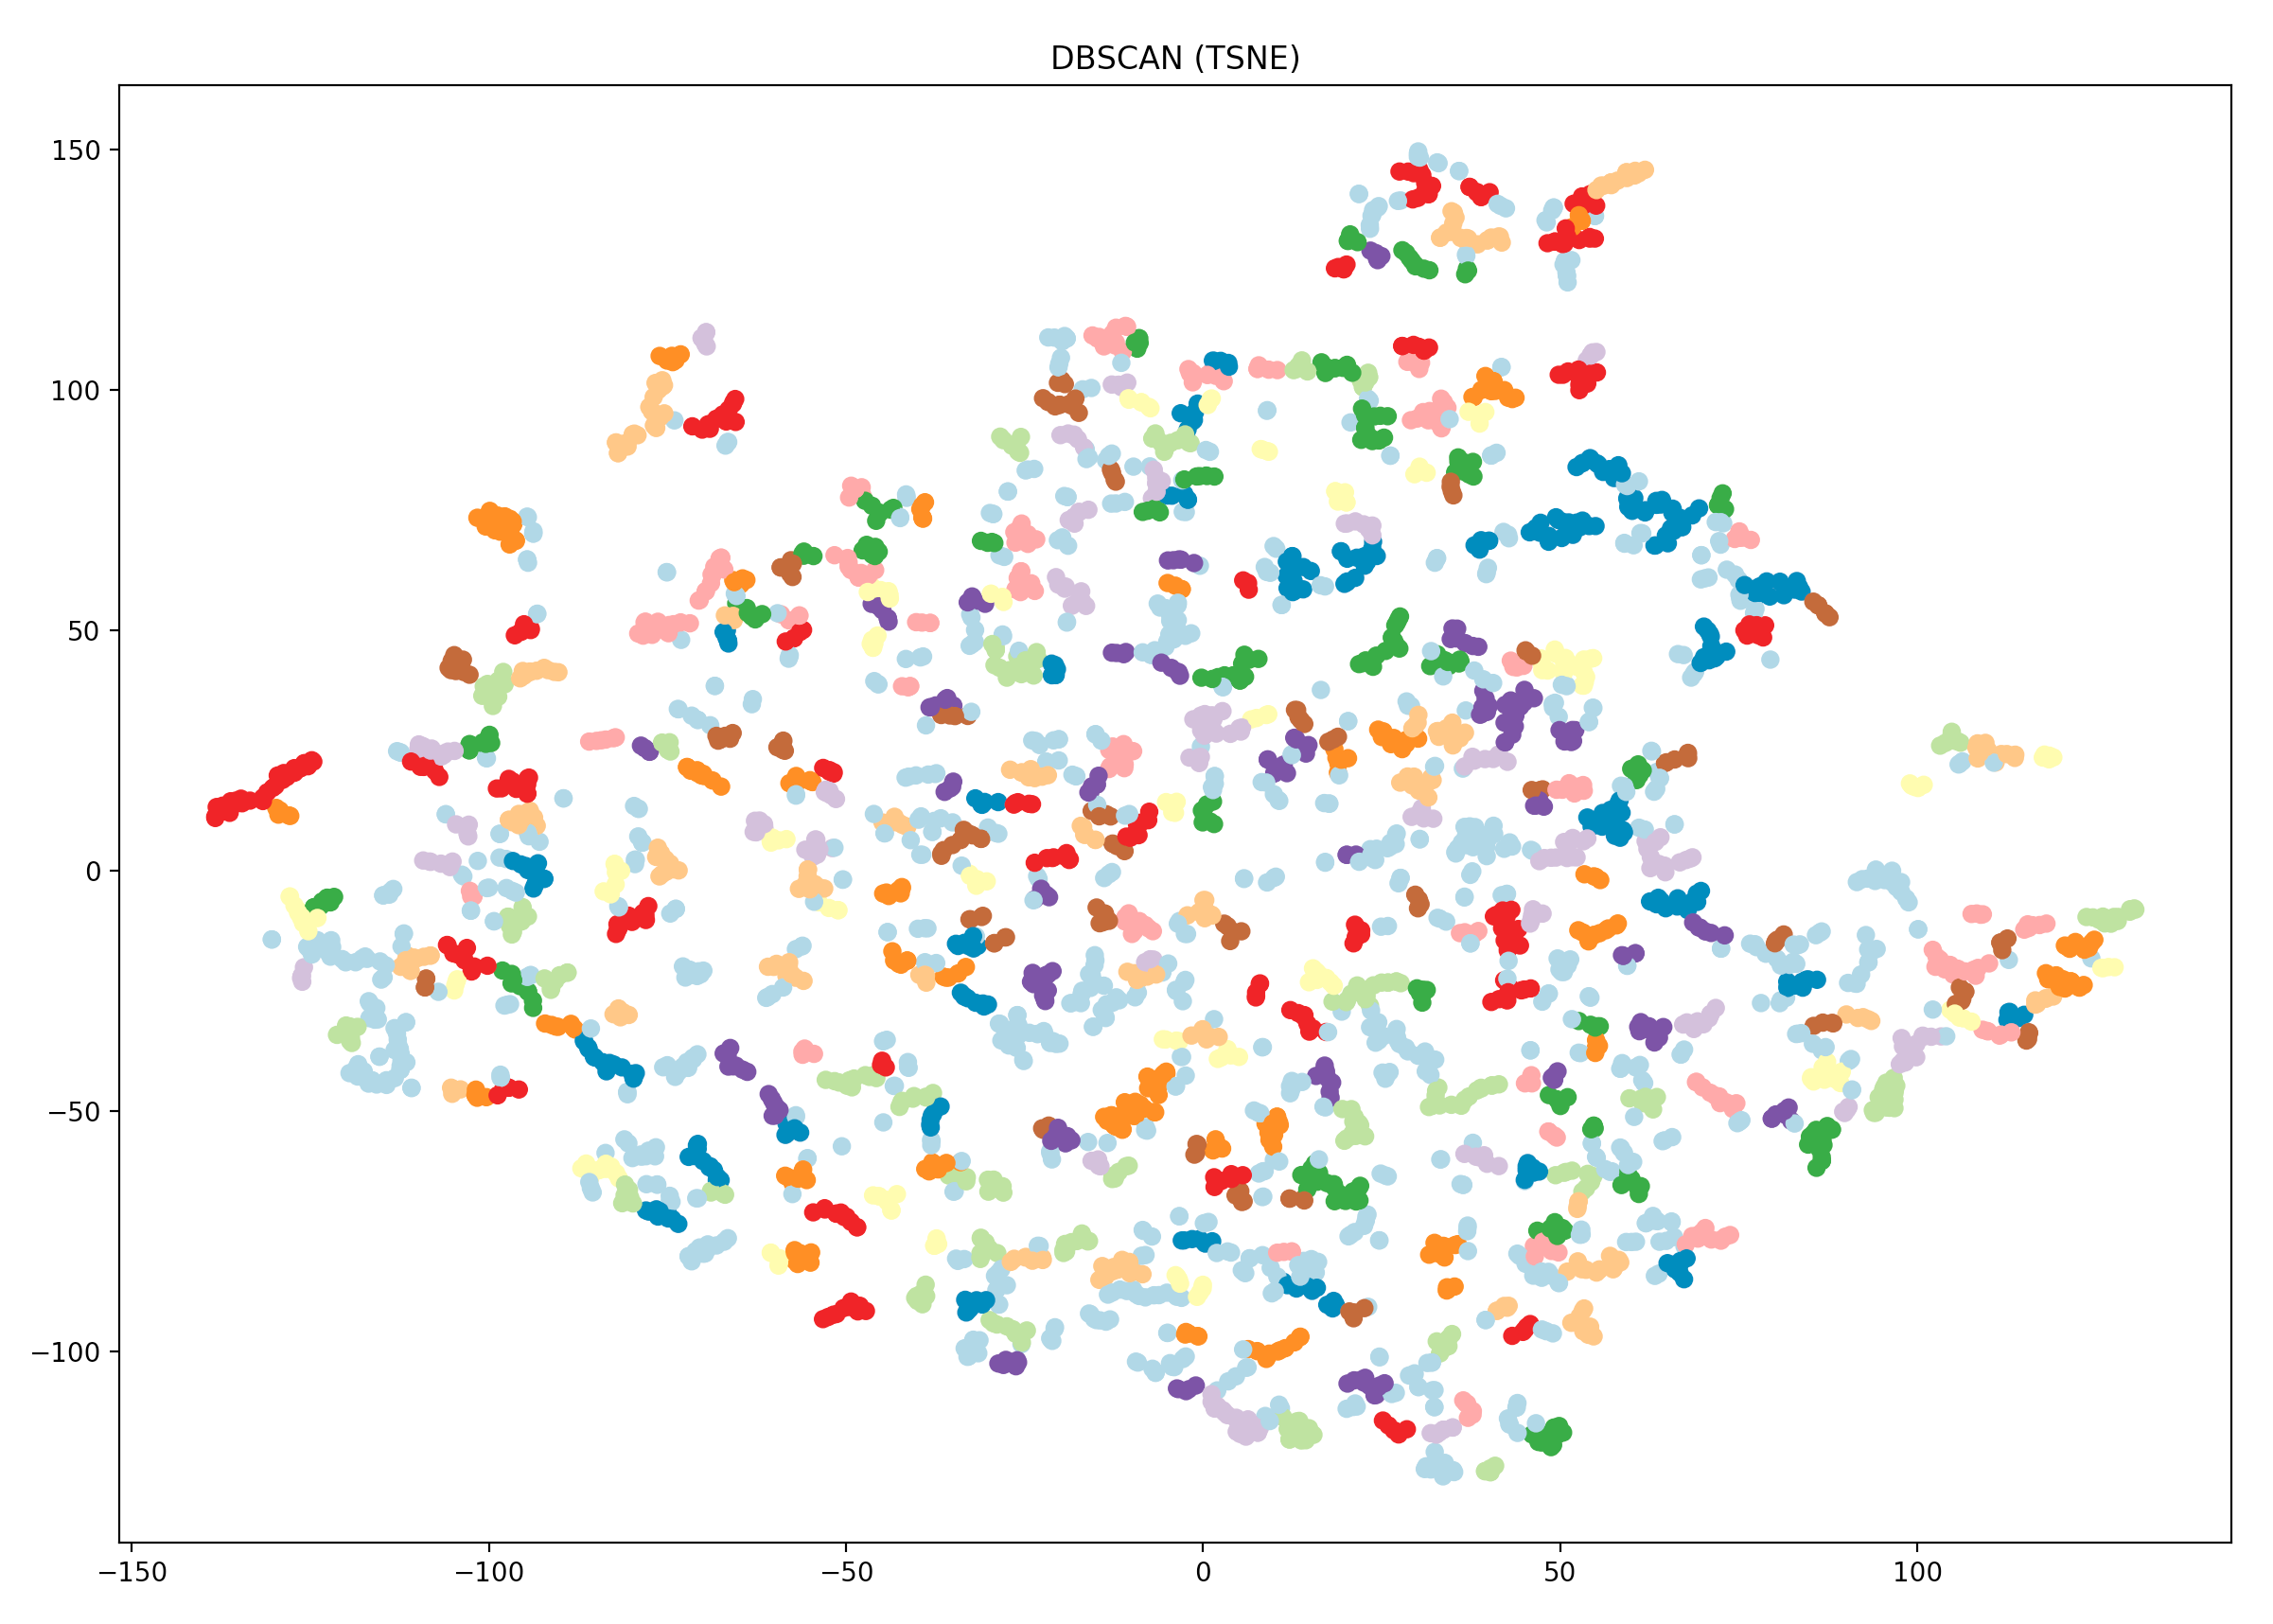
\includegraphics[width=0.9\textwidth]{./images/tsneParametersTest/perplexity/perp10-3hDBSCAN.png}
    % \caption{}
    % \label{figure:}
	\end{subfigure}
	\caption{\textbf{3h} data files, t-SNE calculated with the following parameters: \textbf{perplexity=10}, n\_iter=5000, learning\_rate=50}
  \label{figure:3hperp10TSNE}
\end{figure}

%------------------ PERPLEXITY 20: ------------------
\subsubsection{Perplexity = 20}
% -- 1h, perp 20 --
\begin{figure}[H]
  \centering
  \begin{subfigure}{.5\textwidth}
    \centering
    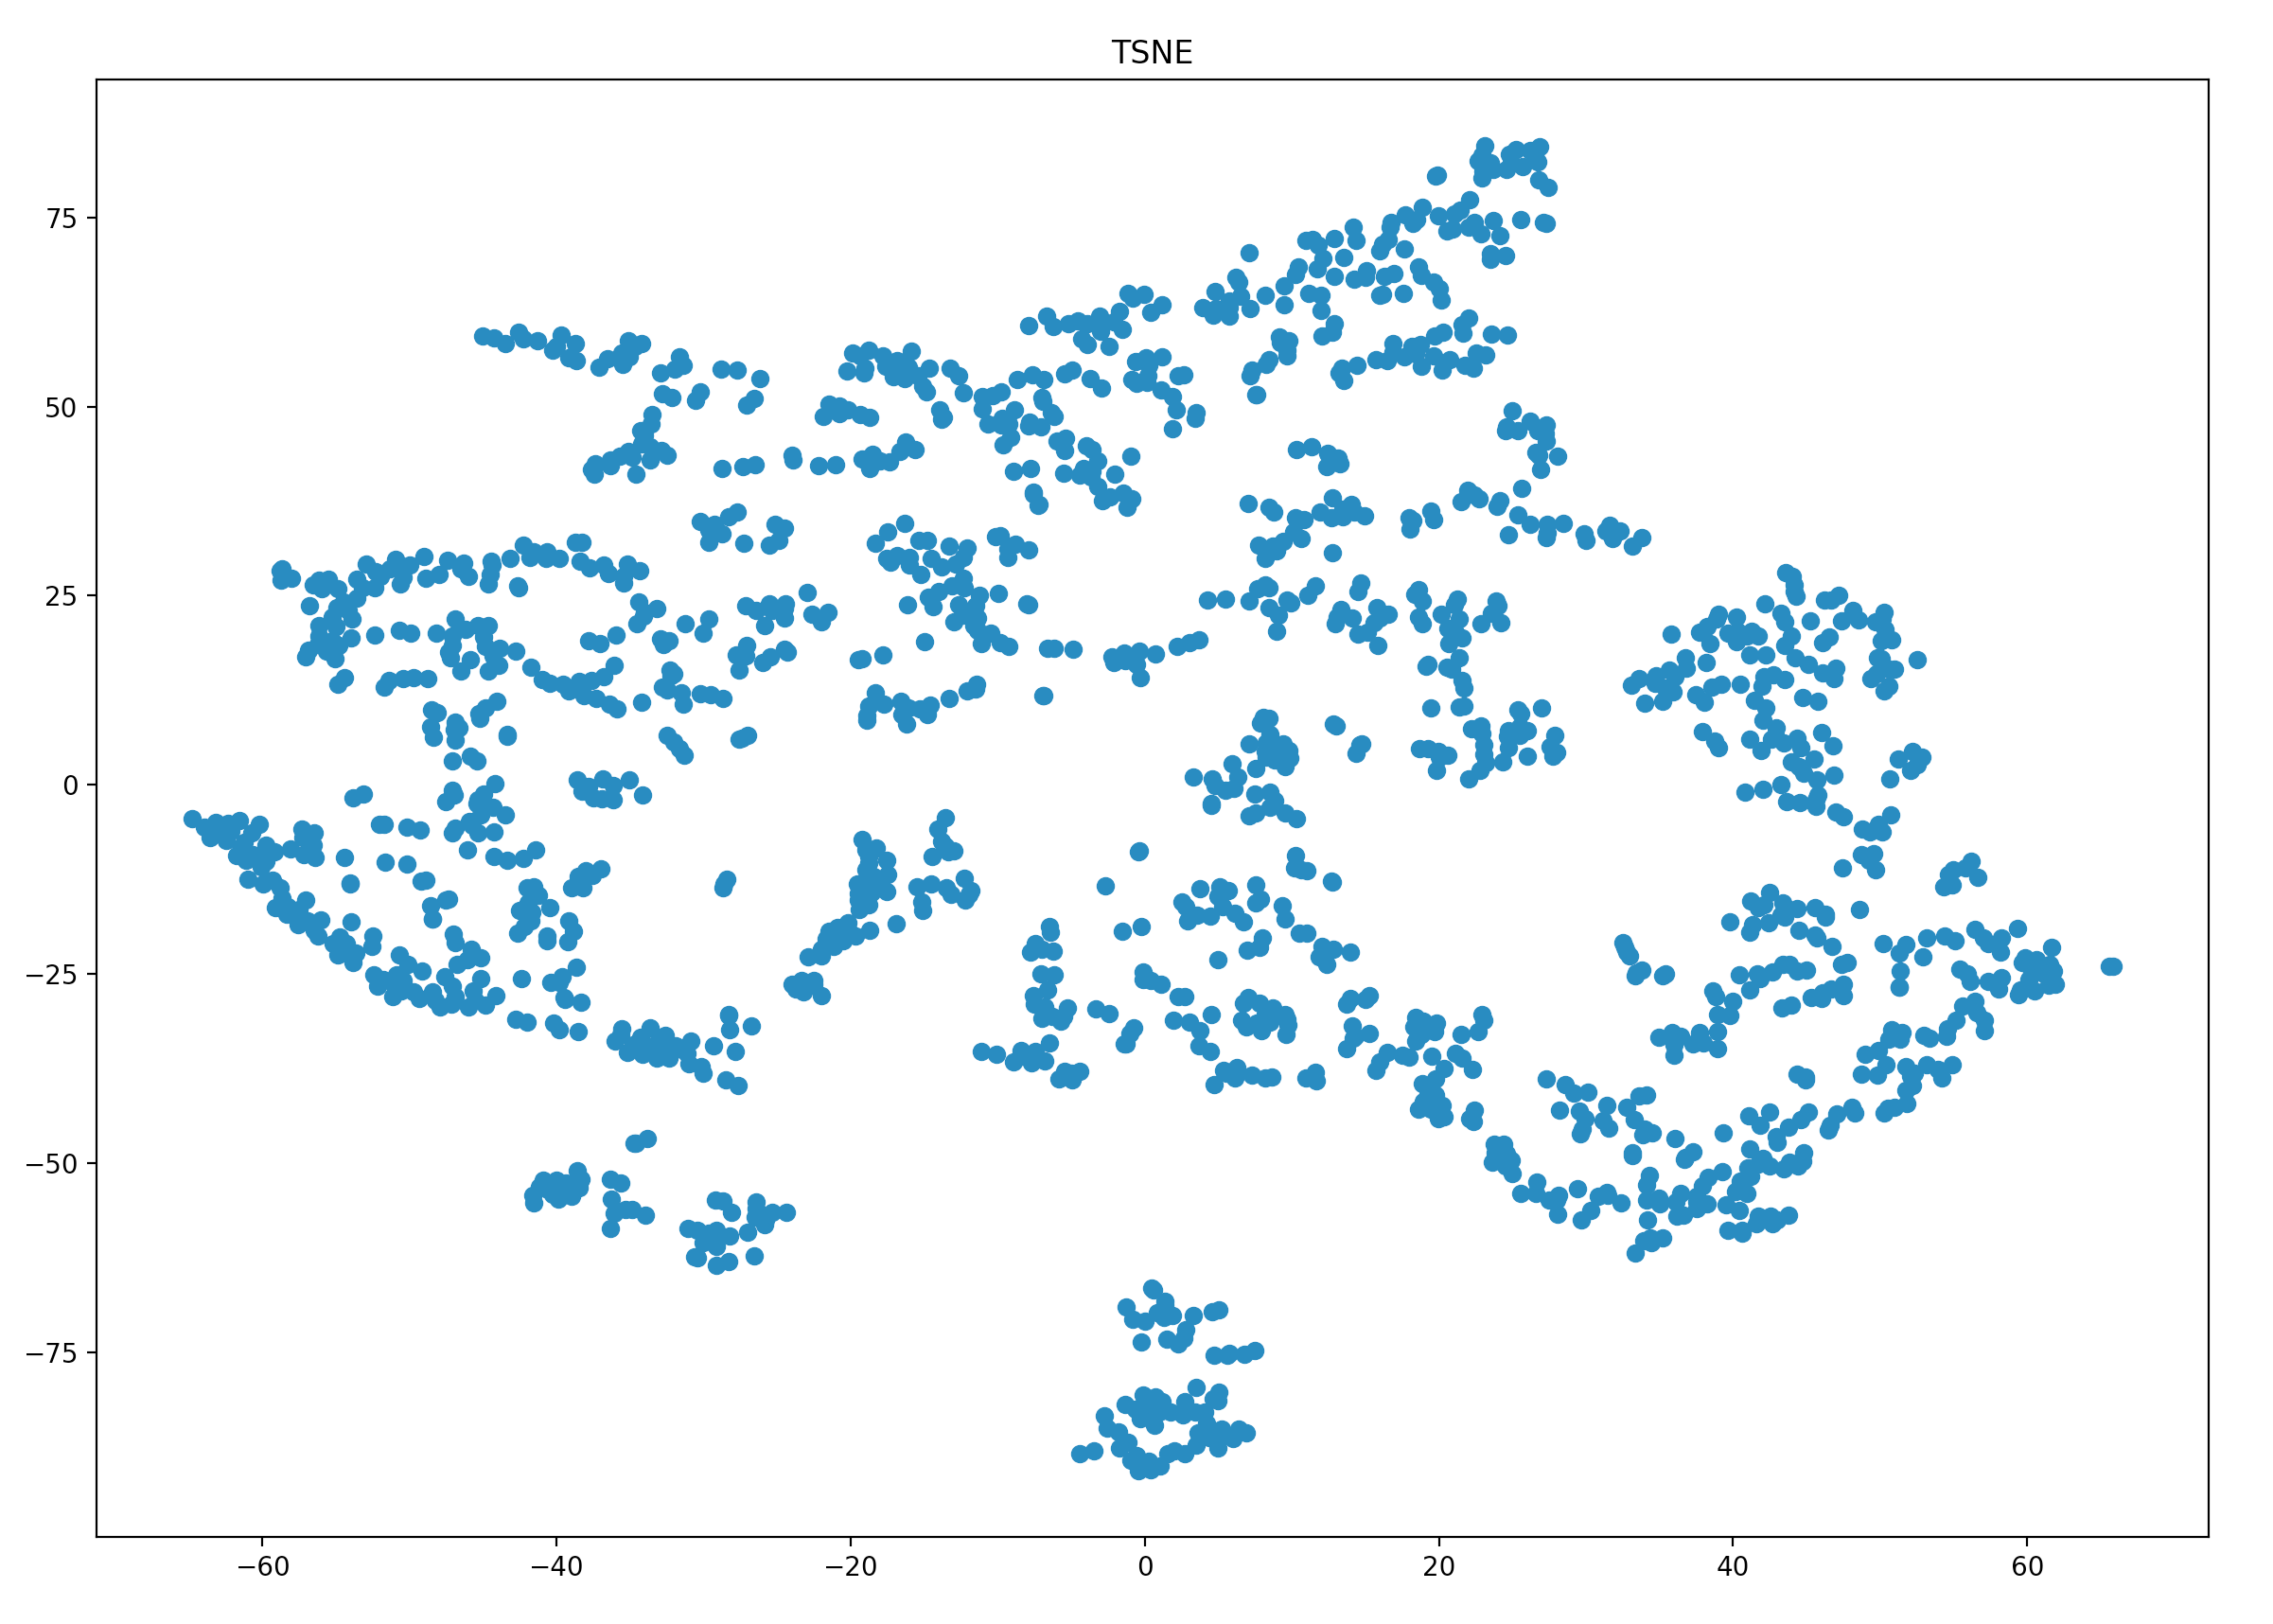
\includegraphics[width=0.9\textwidth]{./images/tsneParametersTest/perplexity/perp20-1hTSNE.png}
  % \caption{}
  % \label{figure:}
  \end{subfigure}%
  \begin{subfigure}{.5\textwidth}
    \centering
    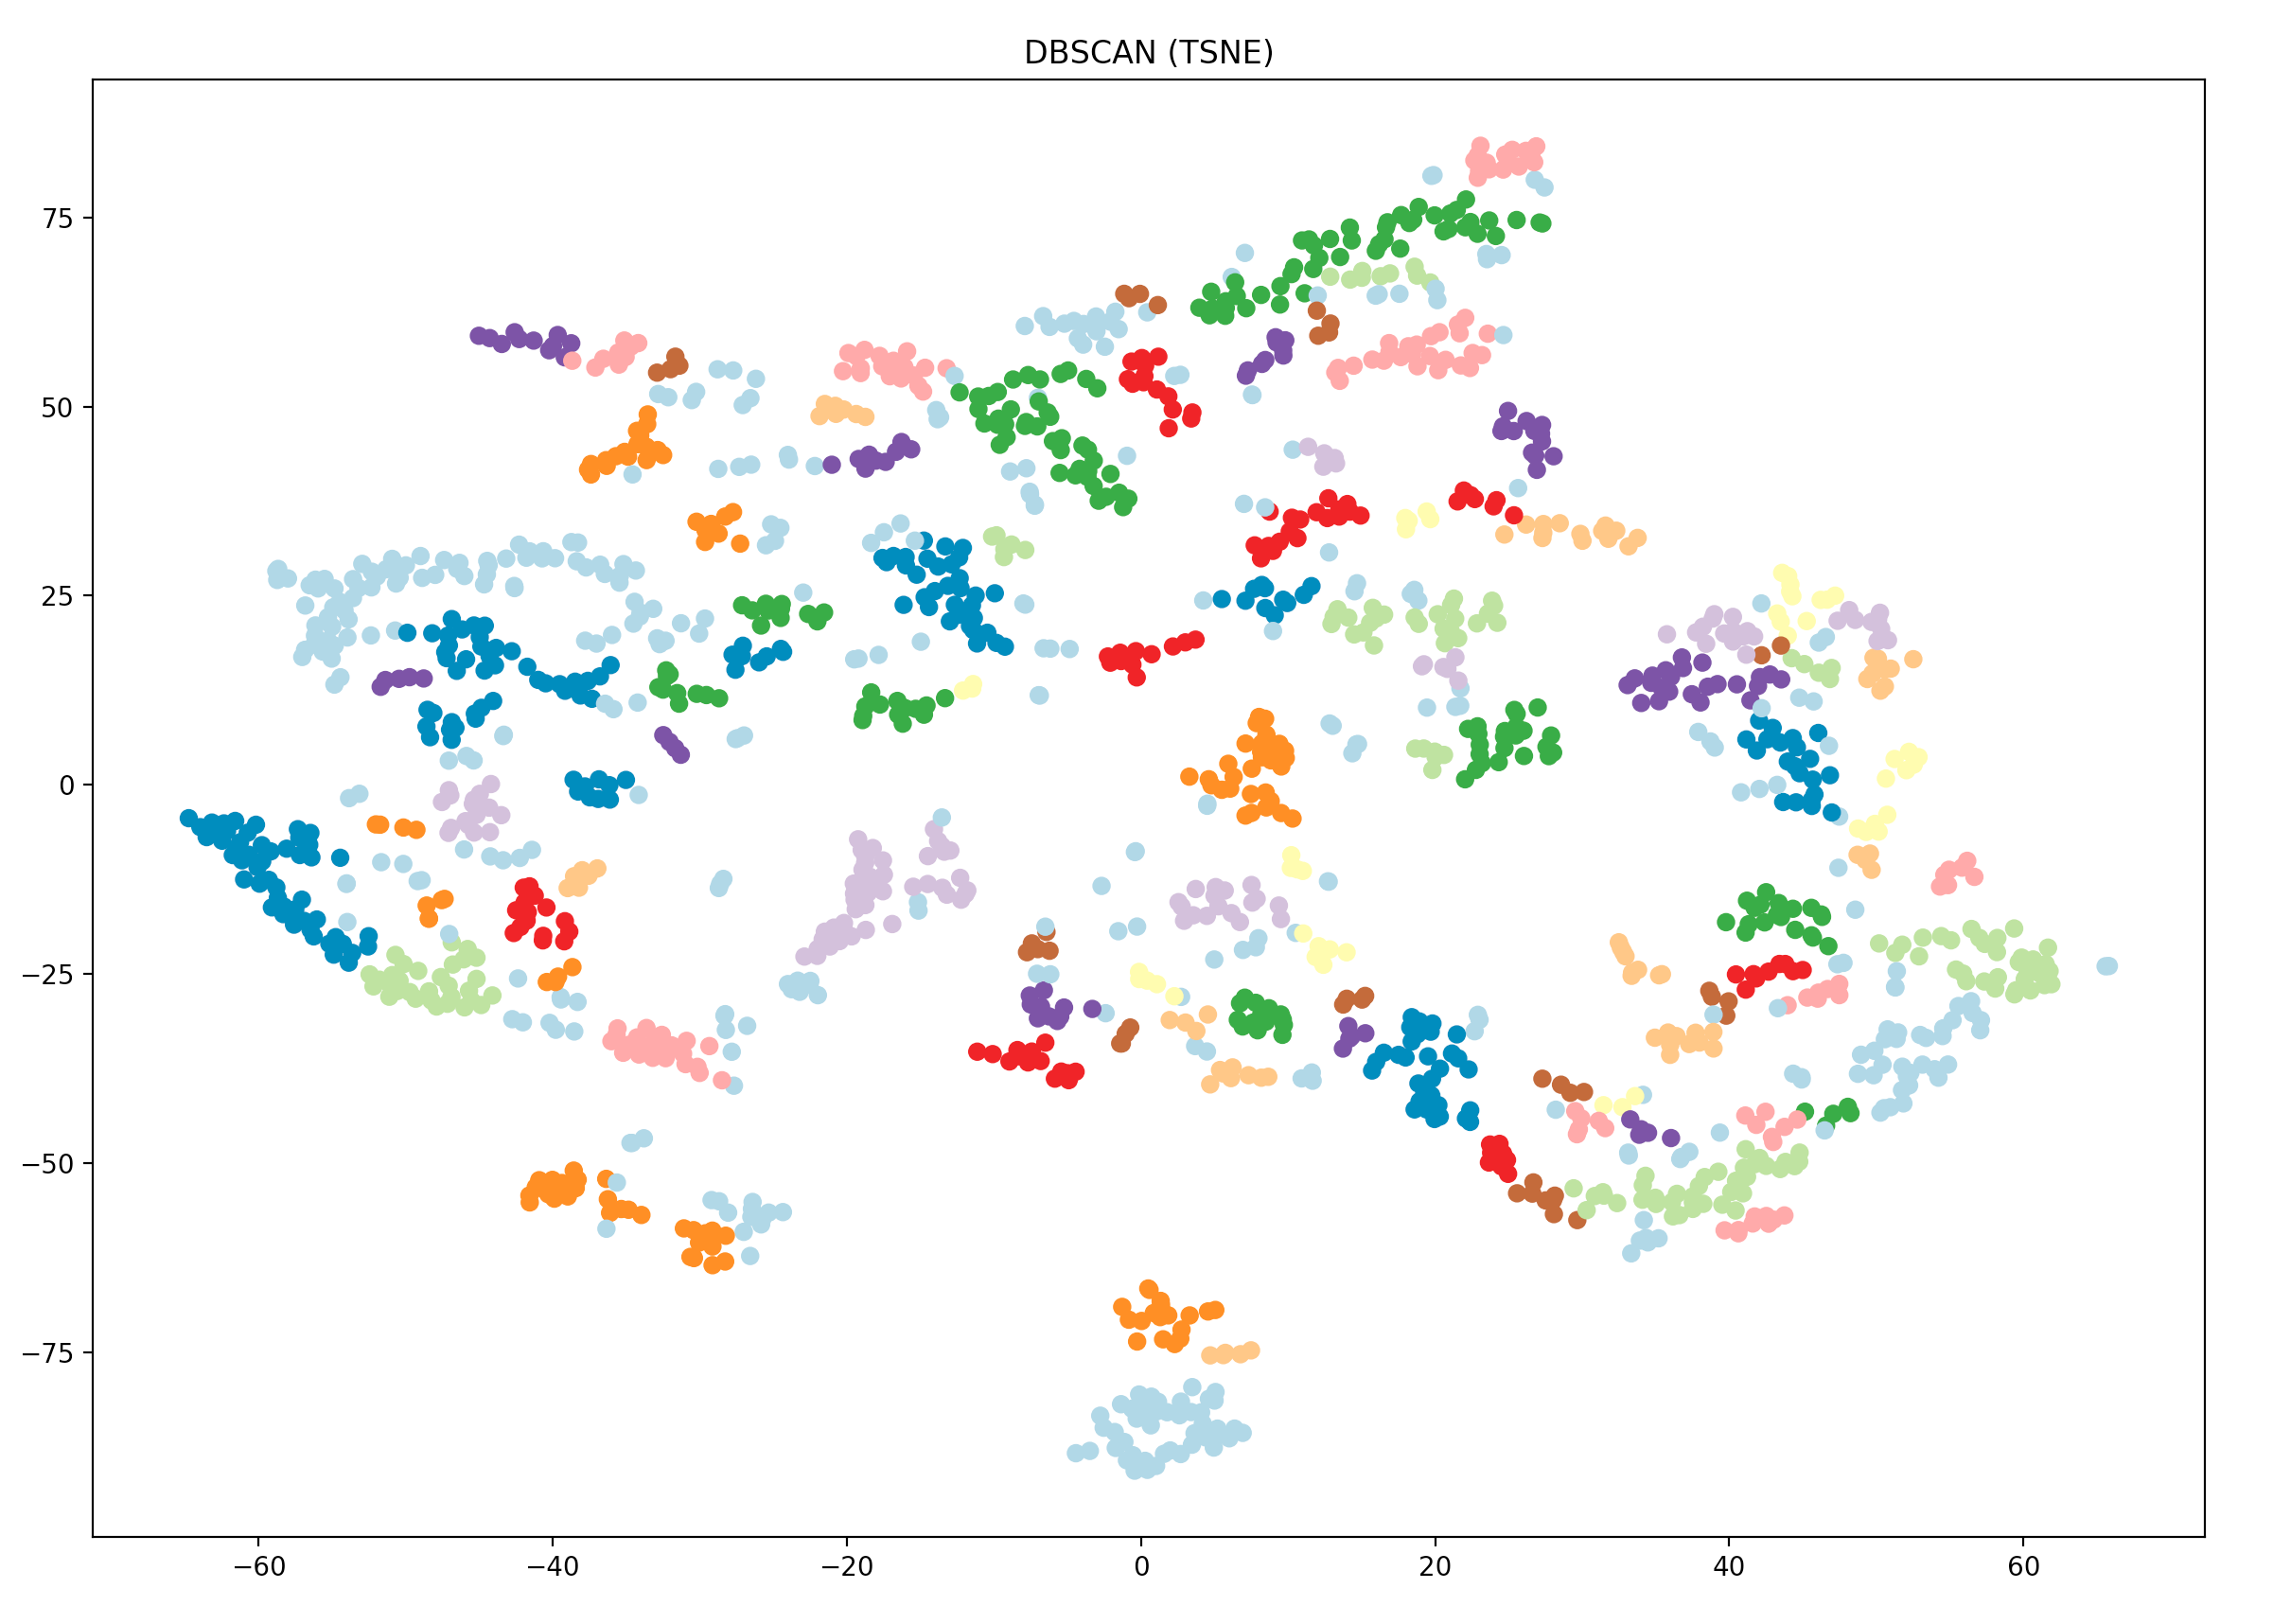
\includegraphics[width=0.9\textwidth]{./images/tsneParametersTest/perplexity/perp20-1hDBSCAN.png}
    % \caption{}
    % \label{figure:}
  \end{subfigure}
	\caption{\textbf{1h} data files, t-SNE calculated with the following parameters: \textbf{perplexity=20}, n\_iter=5000, learning\_rate=50}
  \label{figure:1hperp20TSNE}
\end{figure}

% -- 3h, perp 20 --
\begin{figure}[H]
  \centering
	\begin{subfigure}{.5\textwidth}
    \centering
    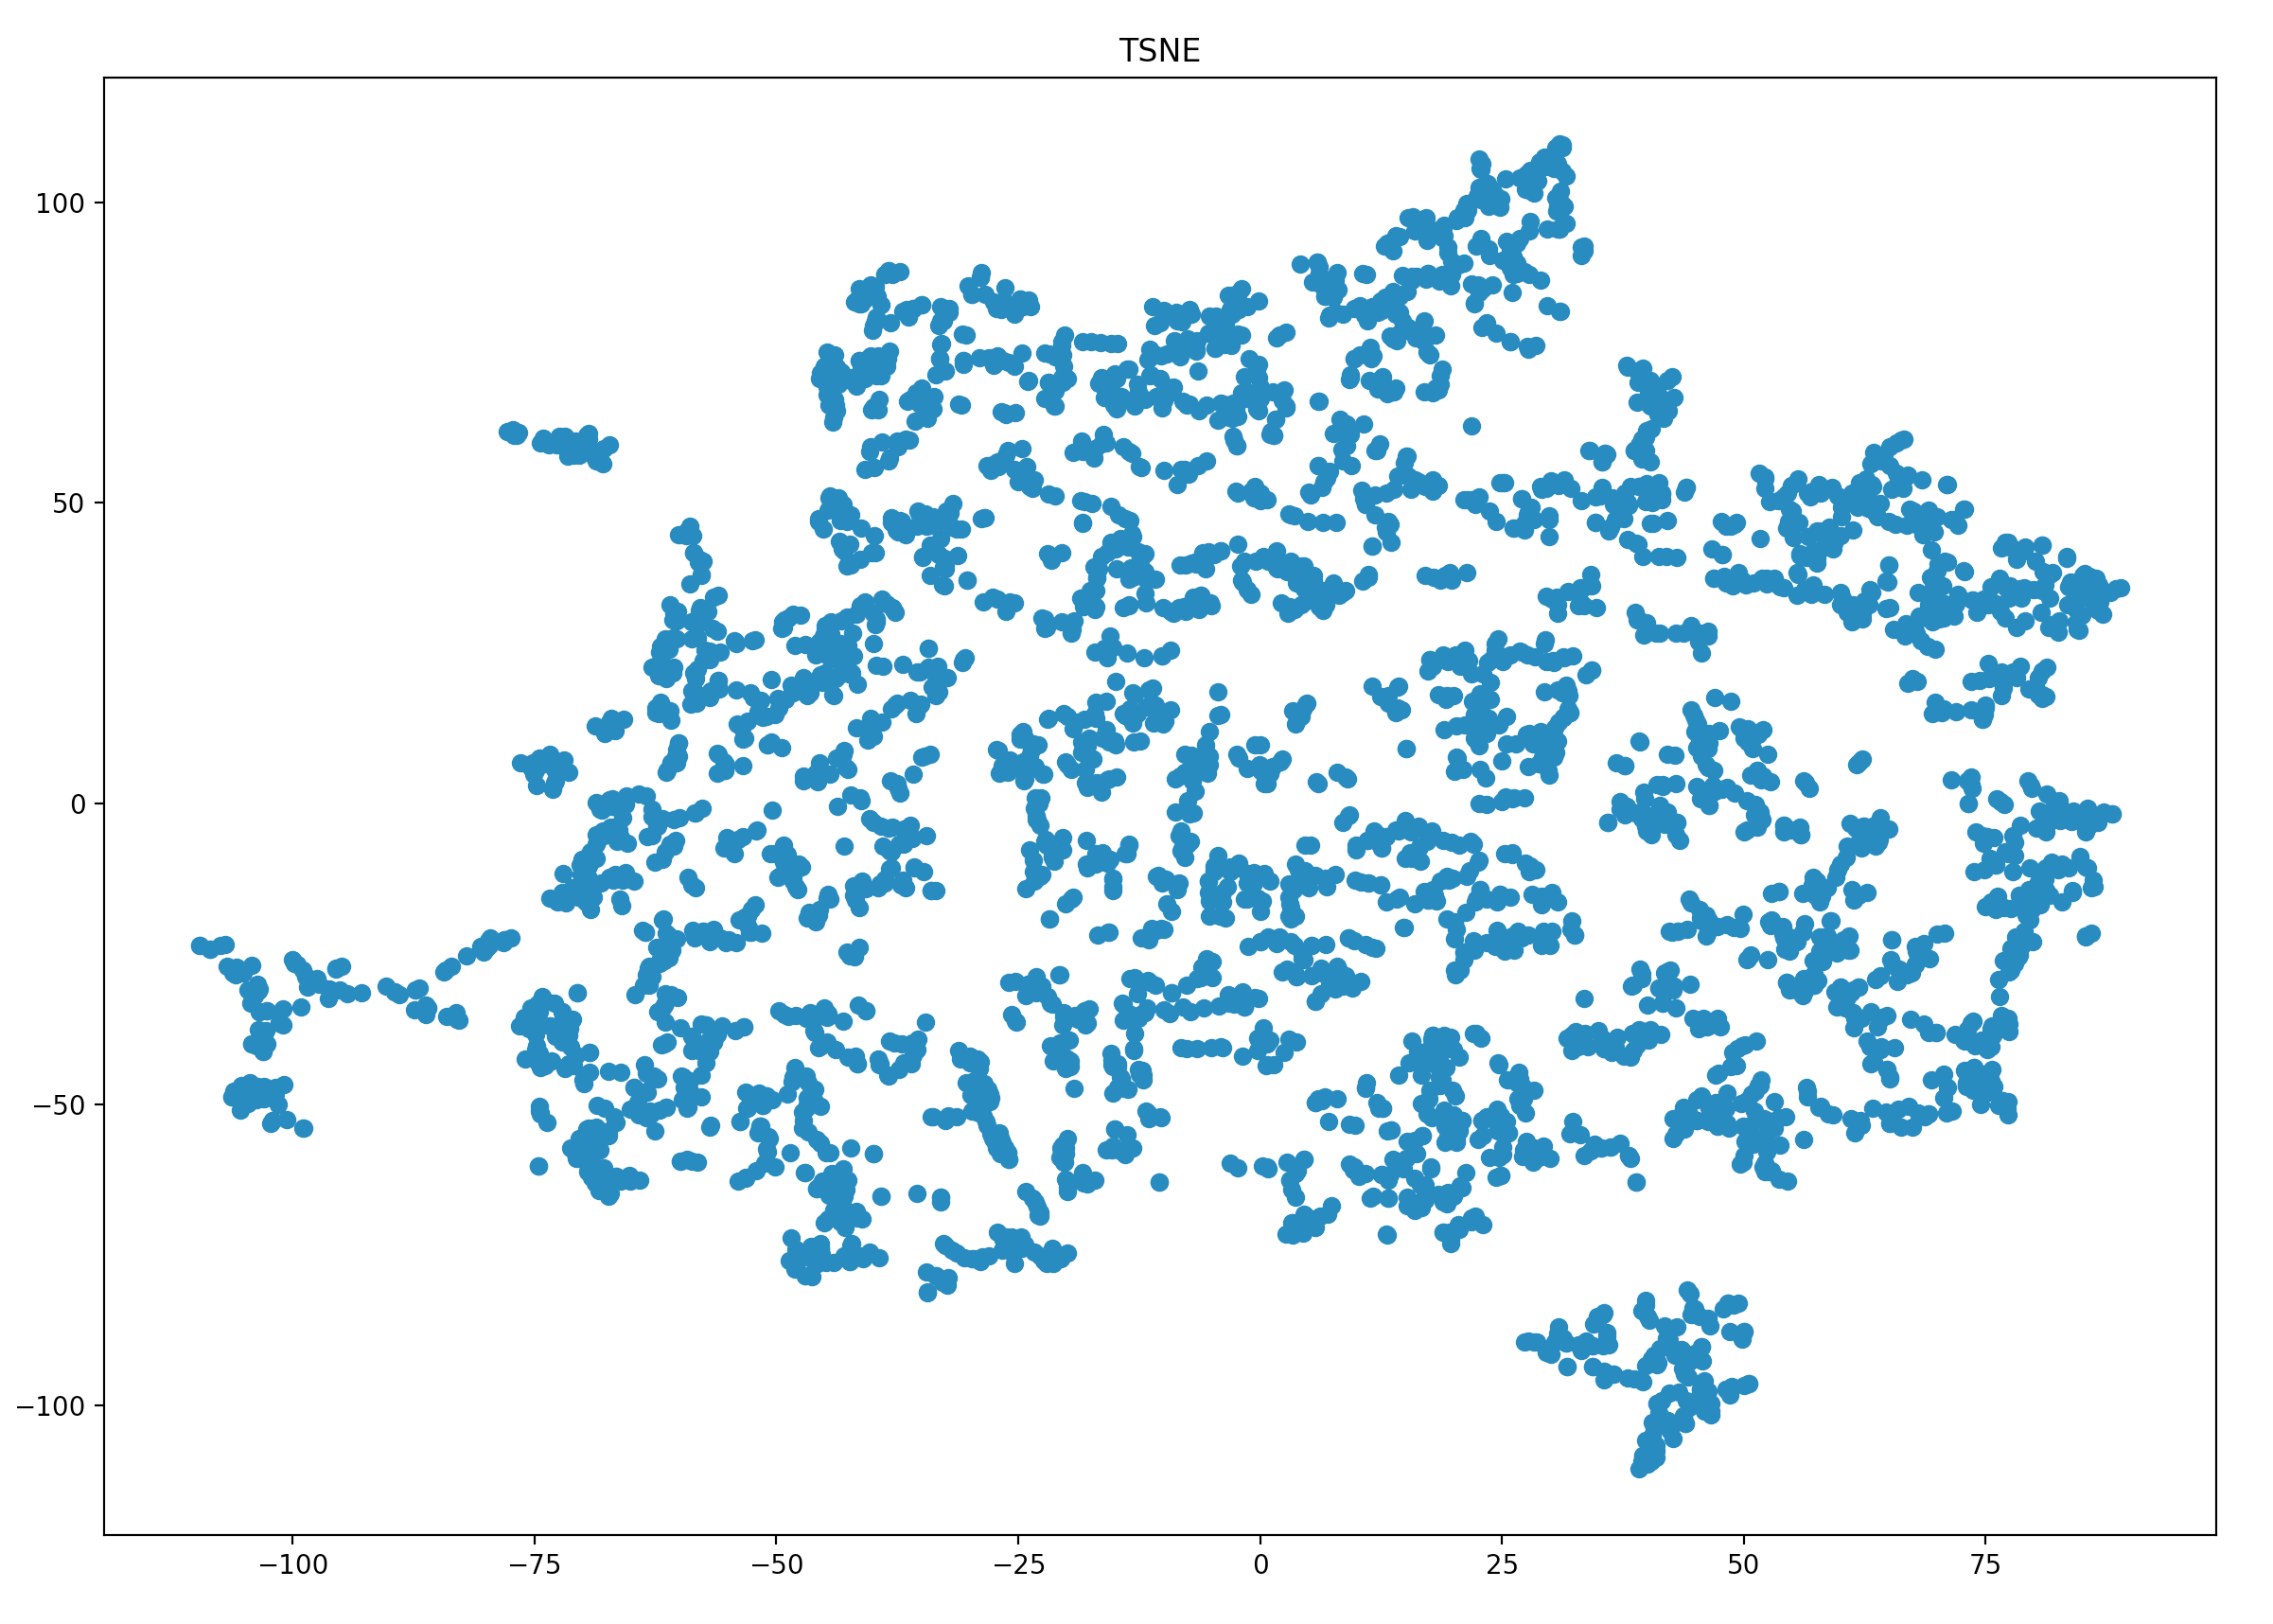
\includegraphics[width=0.9\textwidth]{./images/tsneParametersTest/perplexity/perp20-3hTSNE.png}
  % \caption{}
  % \label{figure:}
  \end{subfigure}%
  \begin{subfigure}{.5\textwidth}
    \centering
    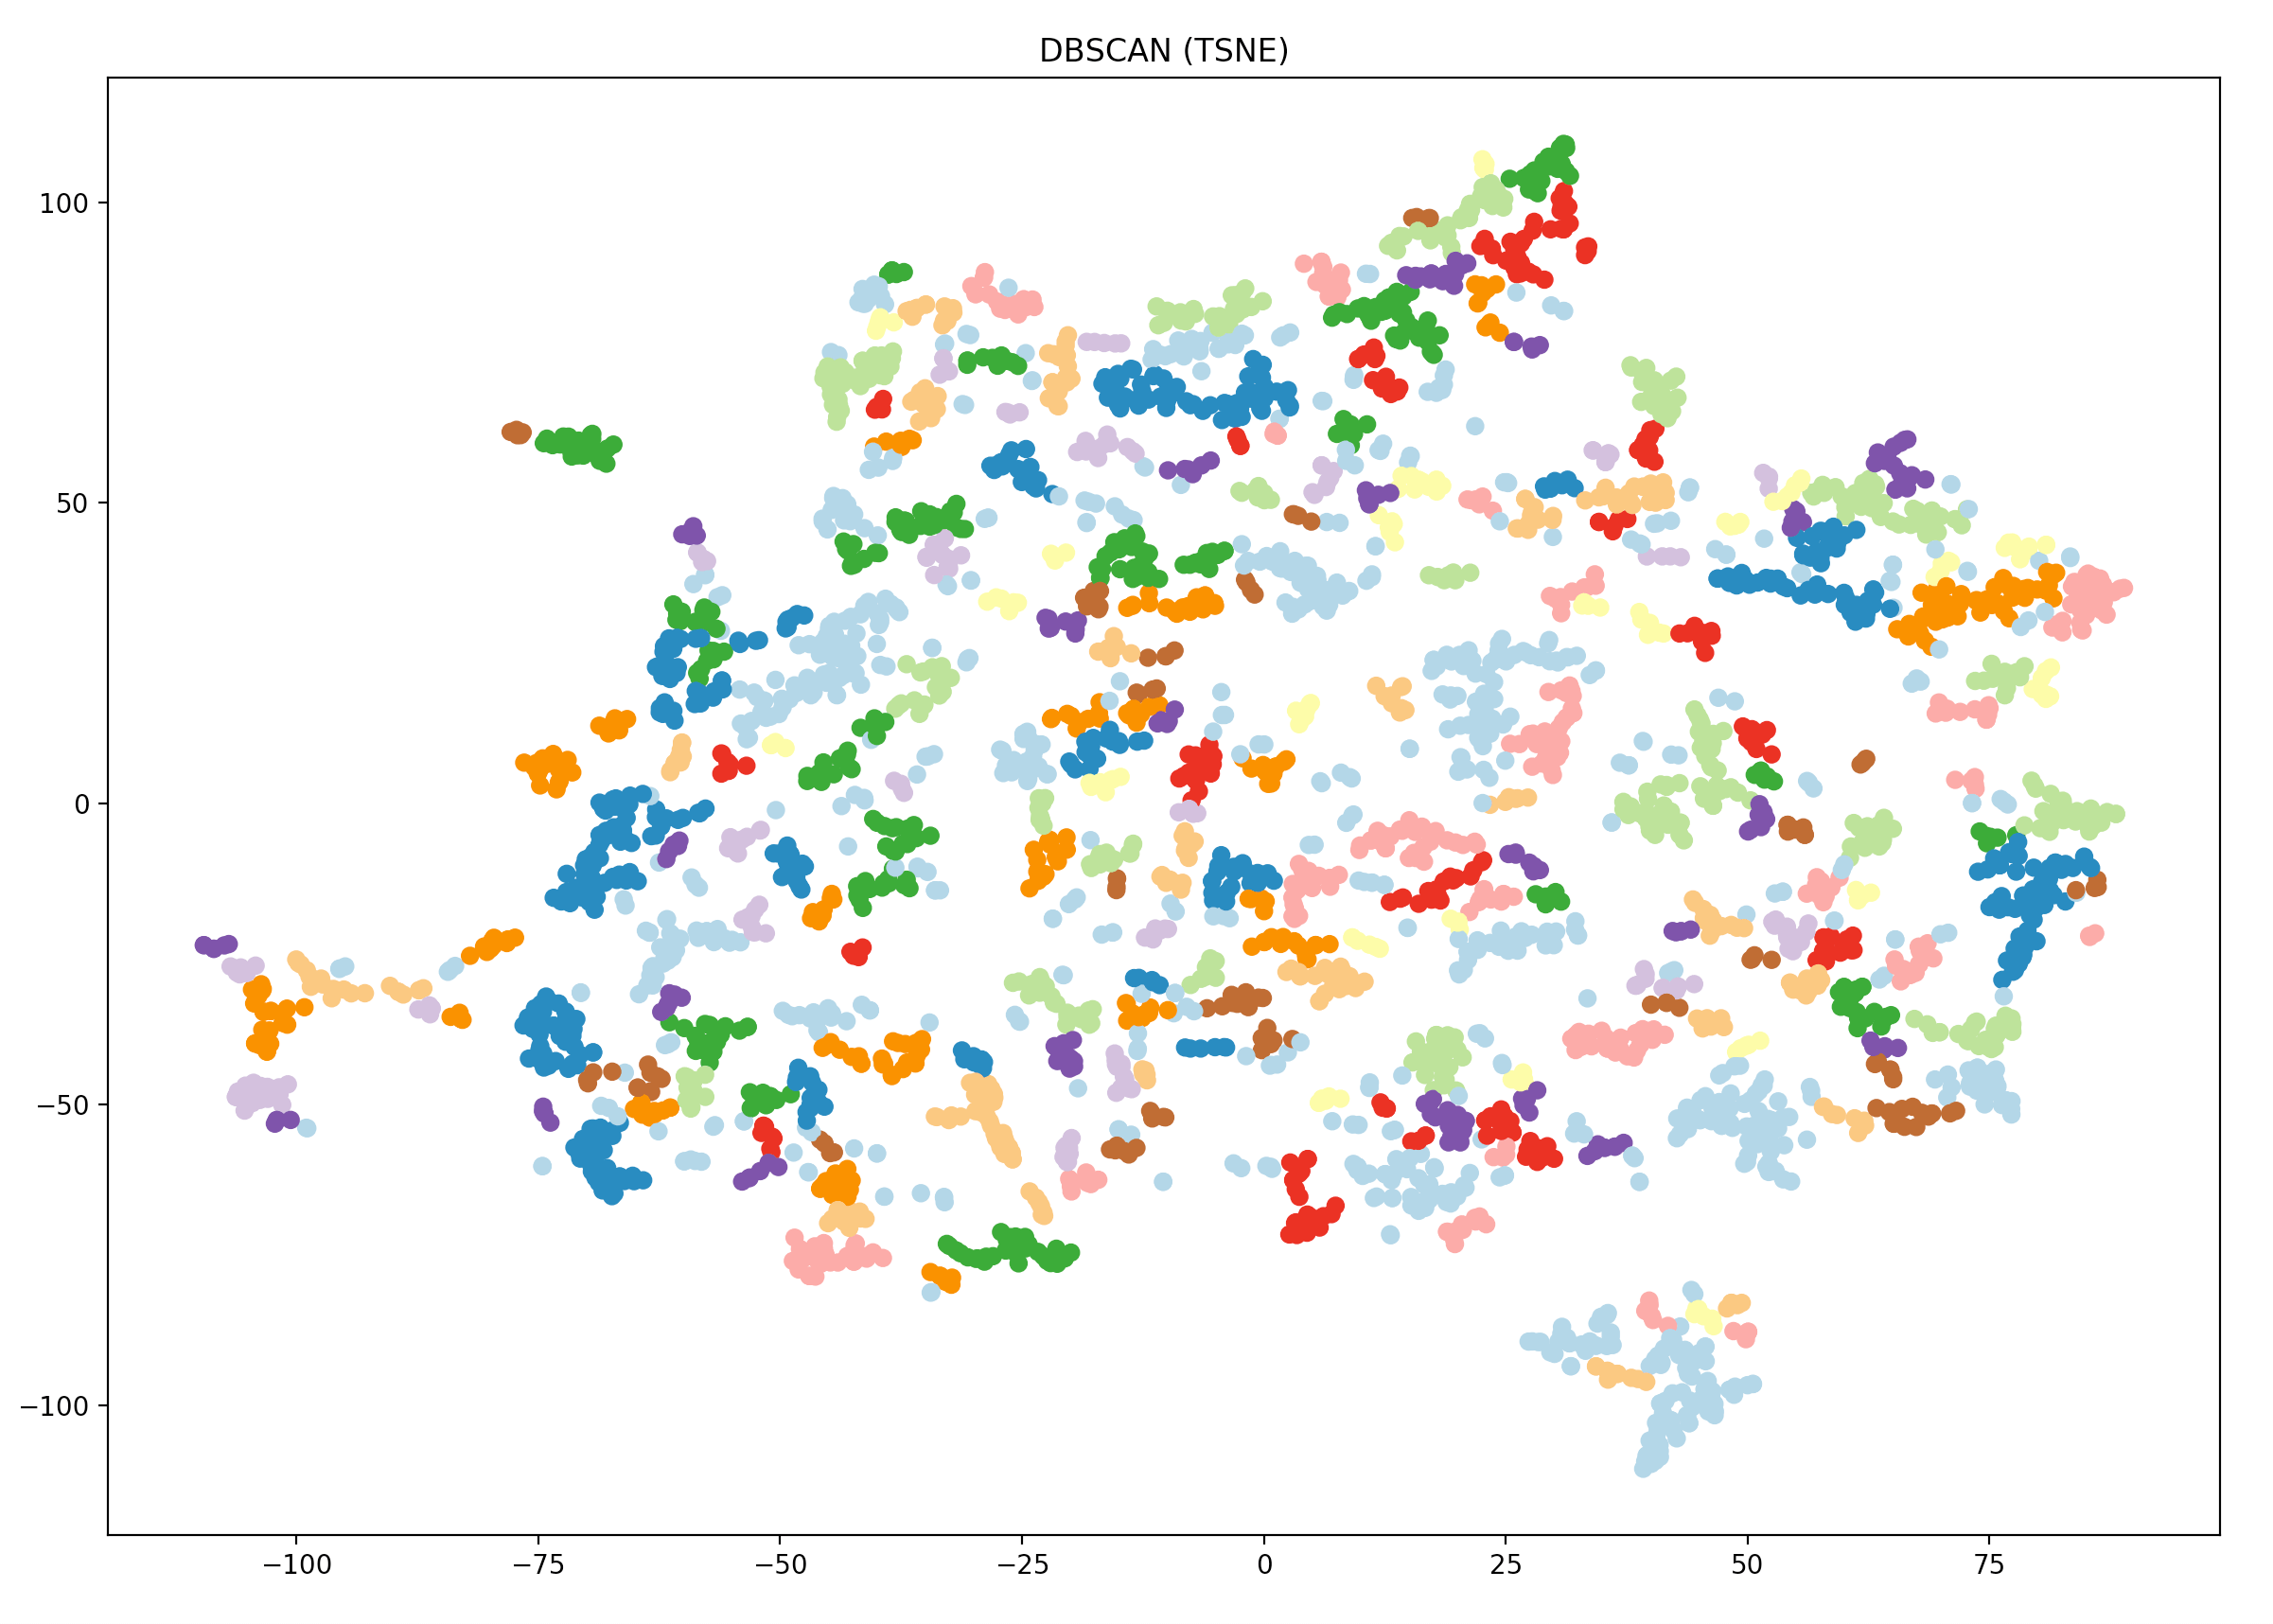
\includegraphics[width=0.9\textwidth]{./images/tsneParametersTest/perplexity/perp20-3hDBSCAN.png}
    % \caption{}
    % \label{figure:}
	\end{subfigure}
	\caption{\textbf{3h} data files, t-SNE calculated with the following parameters: \textbf{perplexity=20}, n\_iter=5000, learning\_rate=50}
  \label{figure:3hperp20TSNE}
\end{figure}



%------------------ PERPLEXITY 30: ------------------
\subsubsection{Perplexity = 30}
% -- 1h, perp 30 --
\begin{figure}[H]
  \centering
  \begin{subfigure}{.5\textwidth}
    \centering
    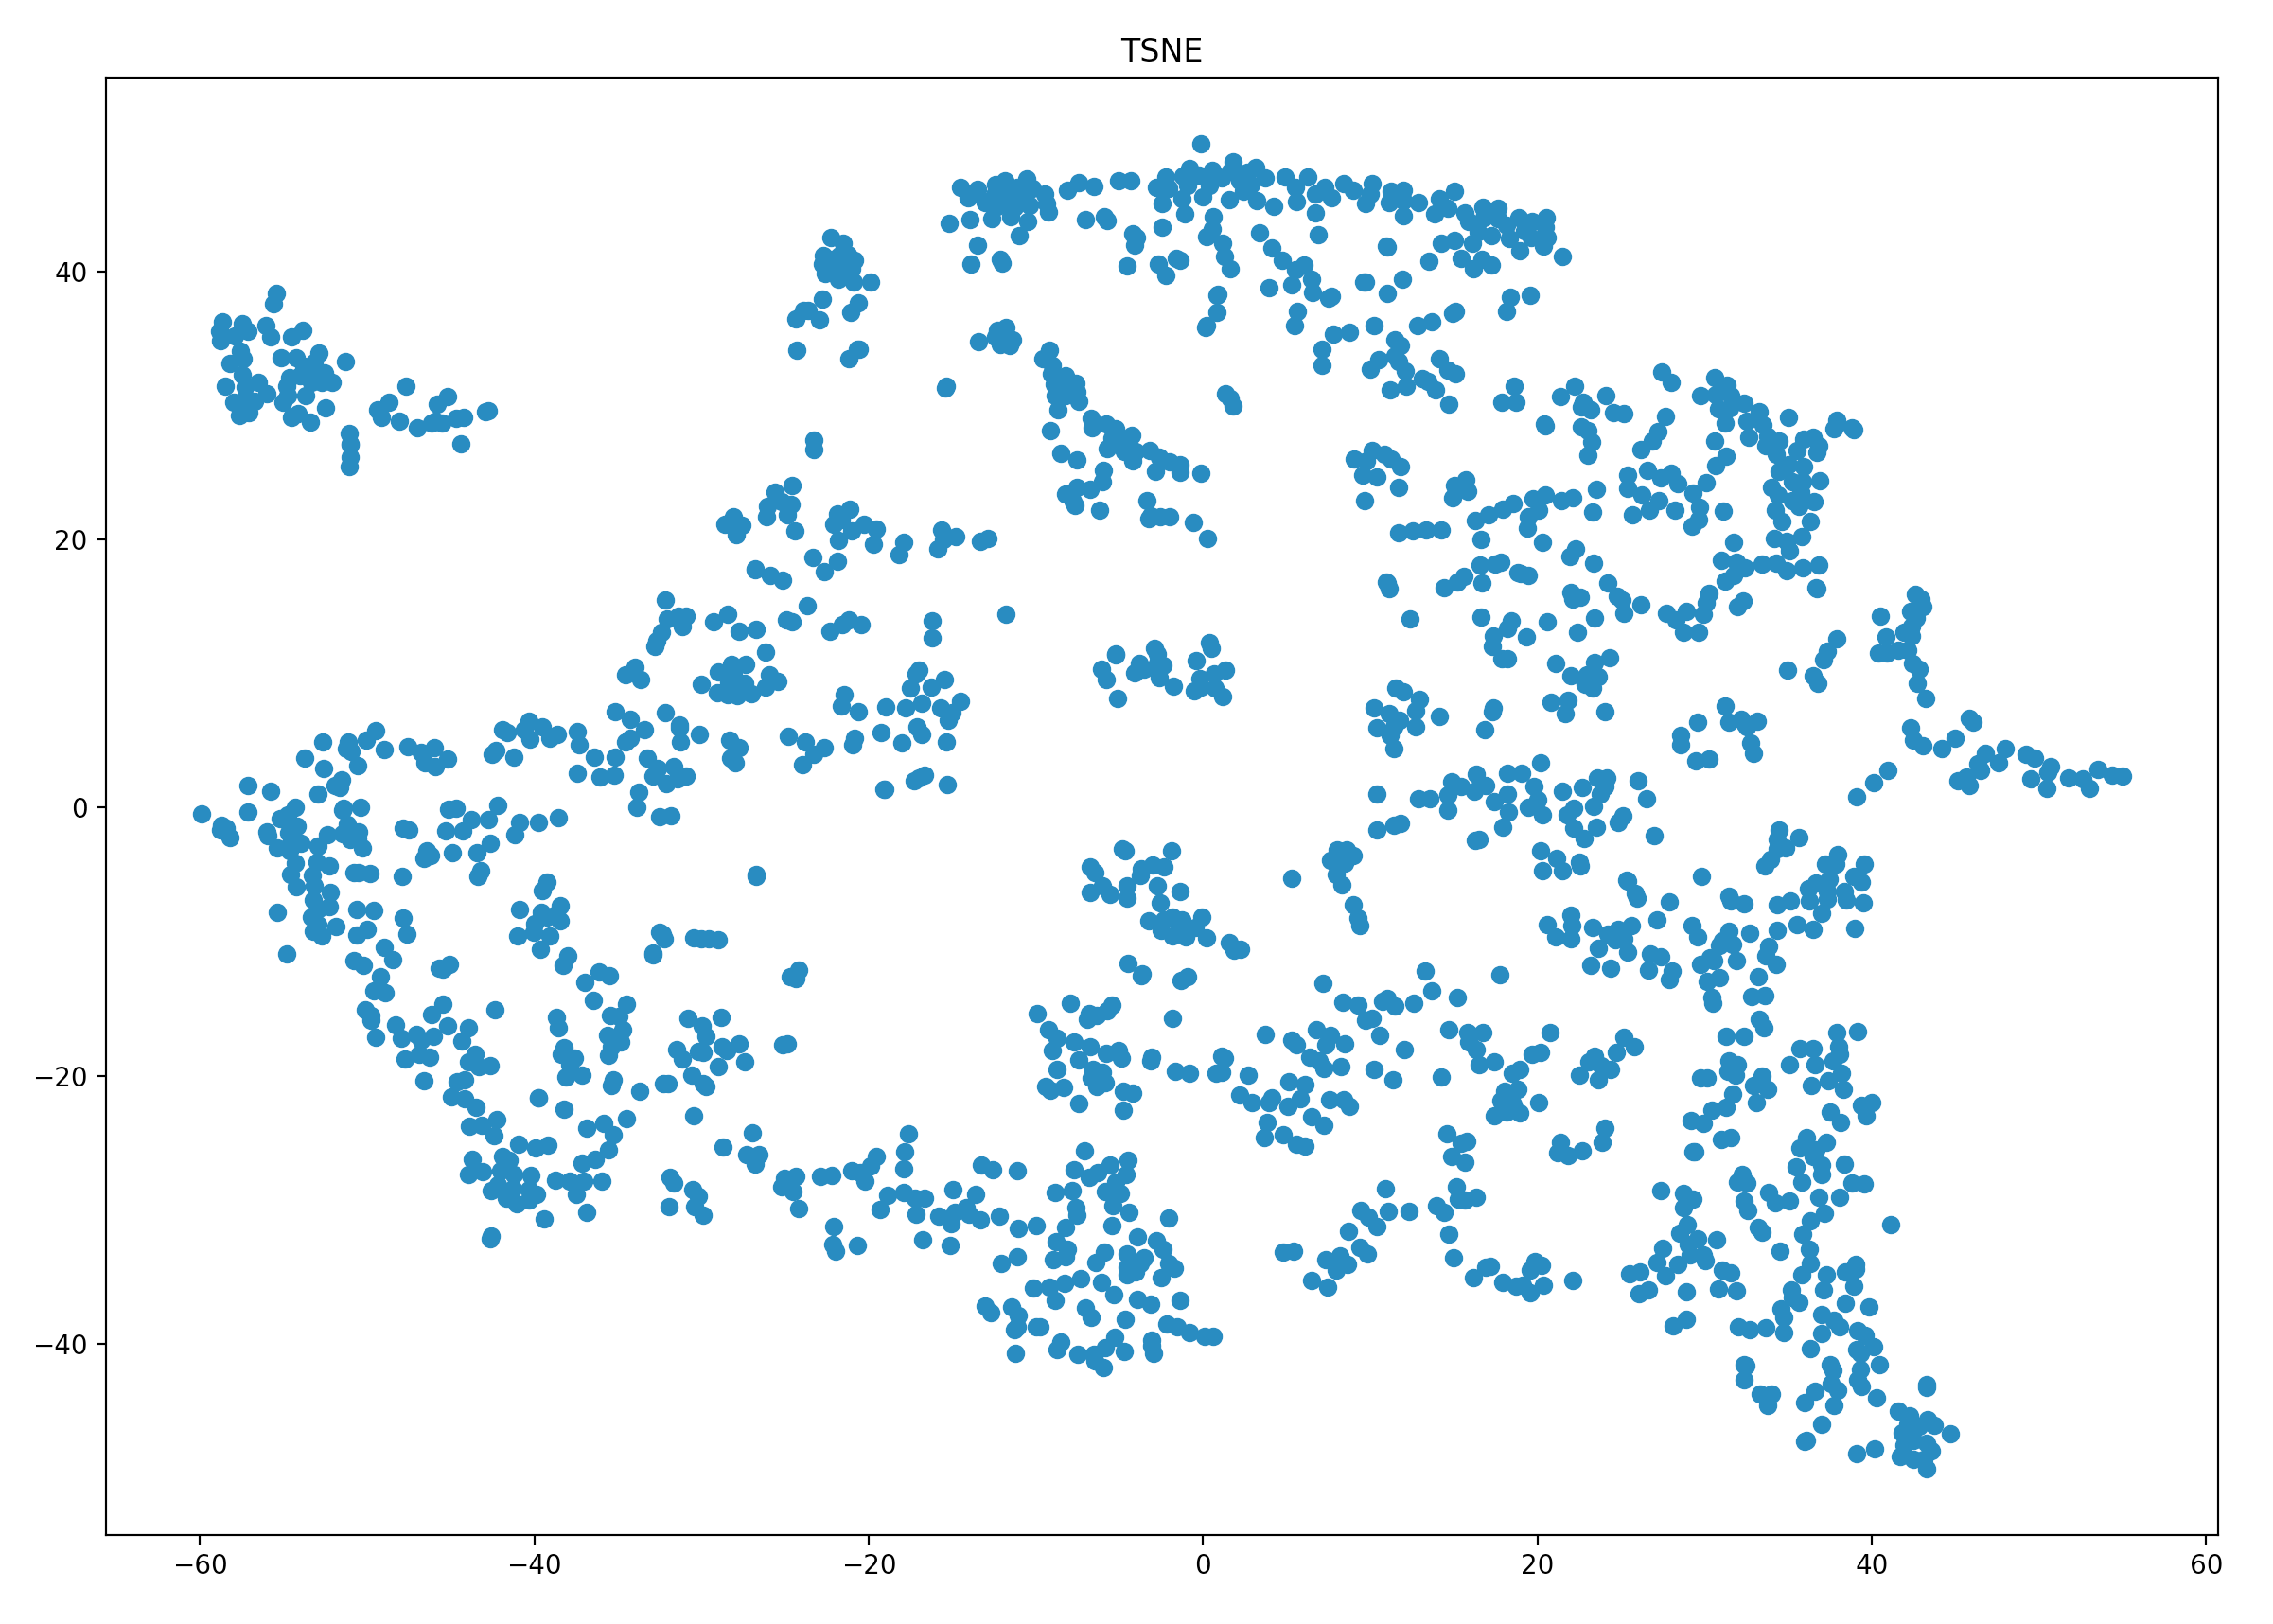
\includegraphics[width=0.9\textwidth]{./images/tsneParametersTest/perplexity/perp30-1hTSNE.png}
  % \caption{}
  % \label{figure:}
  \end{subfigure}%
  \begin{subfigure}{.5\textwidth}
    \centering
    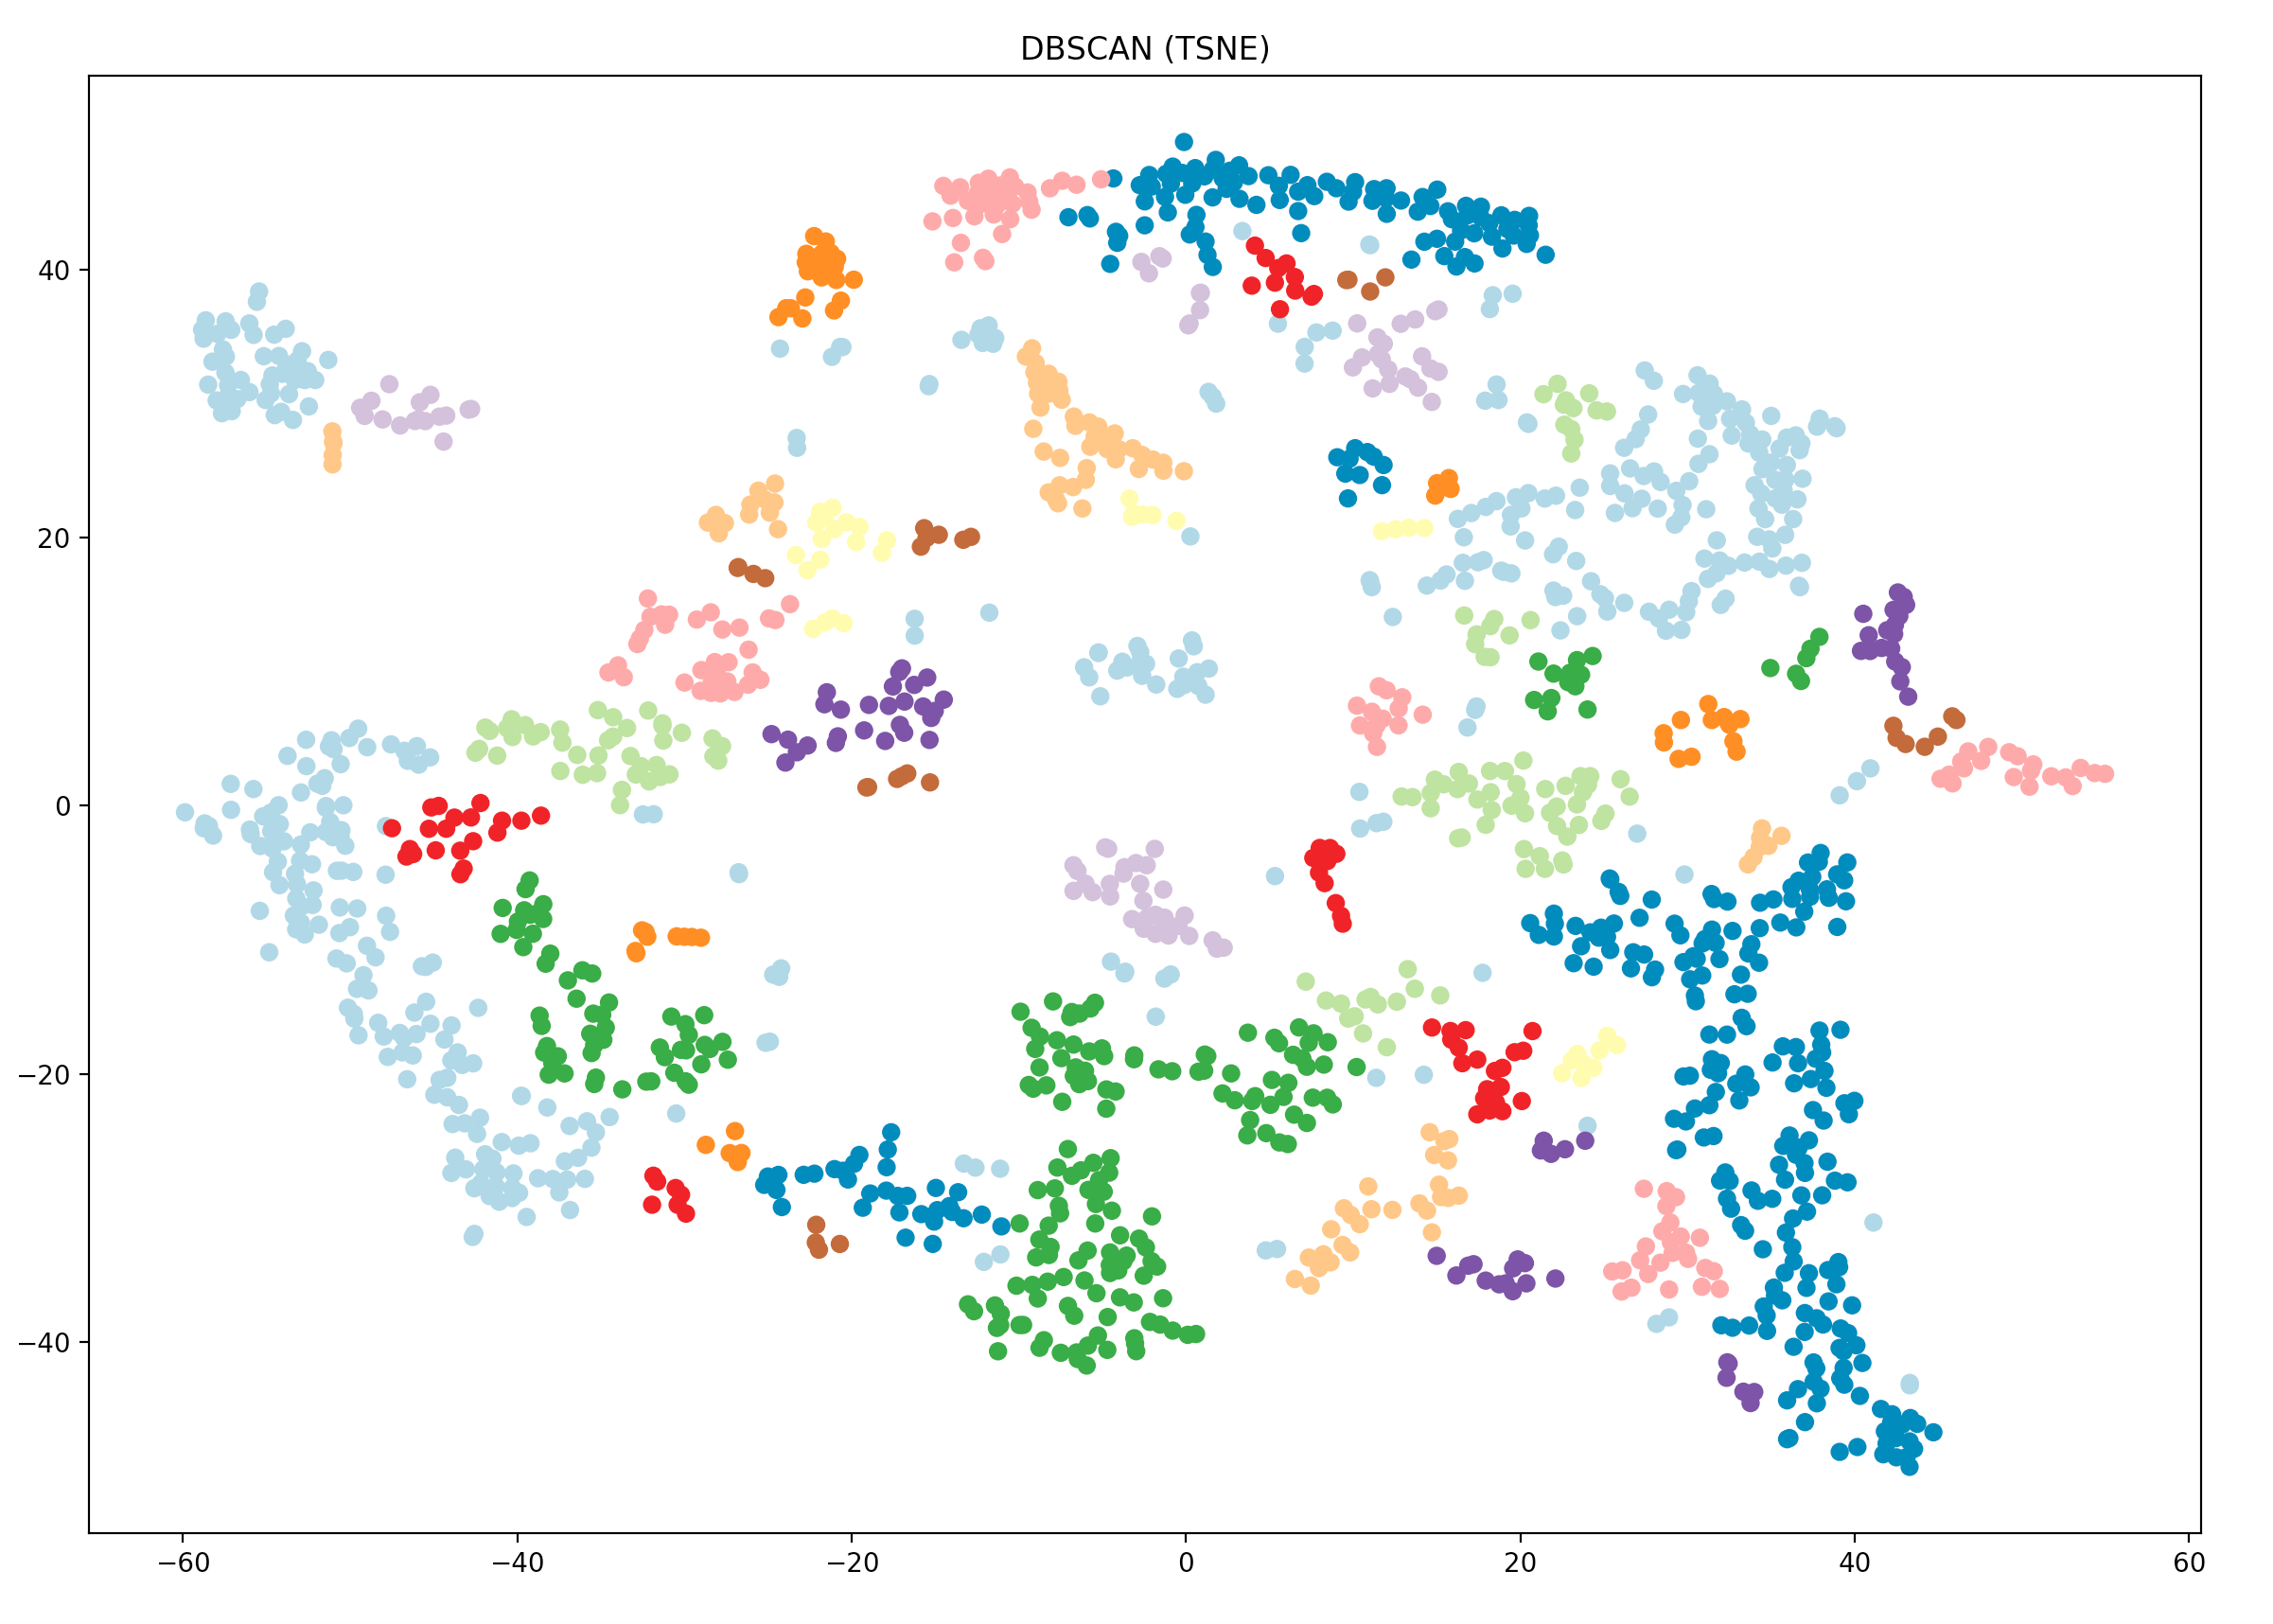
\includegraphics[width=0.9\textwidth]{./images/tsneParametersTest/perplexity/perp30-1hDBSCAN.png}
    % \caption{}
    % \label{figure:}
  \end{subfigure}
	\caption{\textbf{1h} data files, t-SNE calculated with the following parameters: \textbf{perplexity=30}, n\_iter=5000, learning\_rate=50}
  \label{figure:1hperp30TSNE}
\end{figure}

% -- 3h, perp 30 --
\begin{figure}[H]
  \centering
	\begin{subfigure}{.5\textwidth}
    \centering
    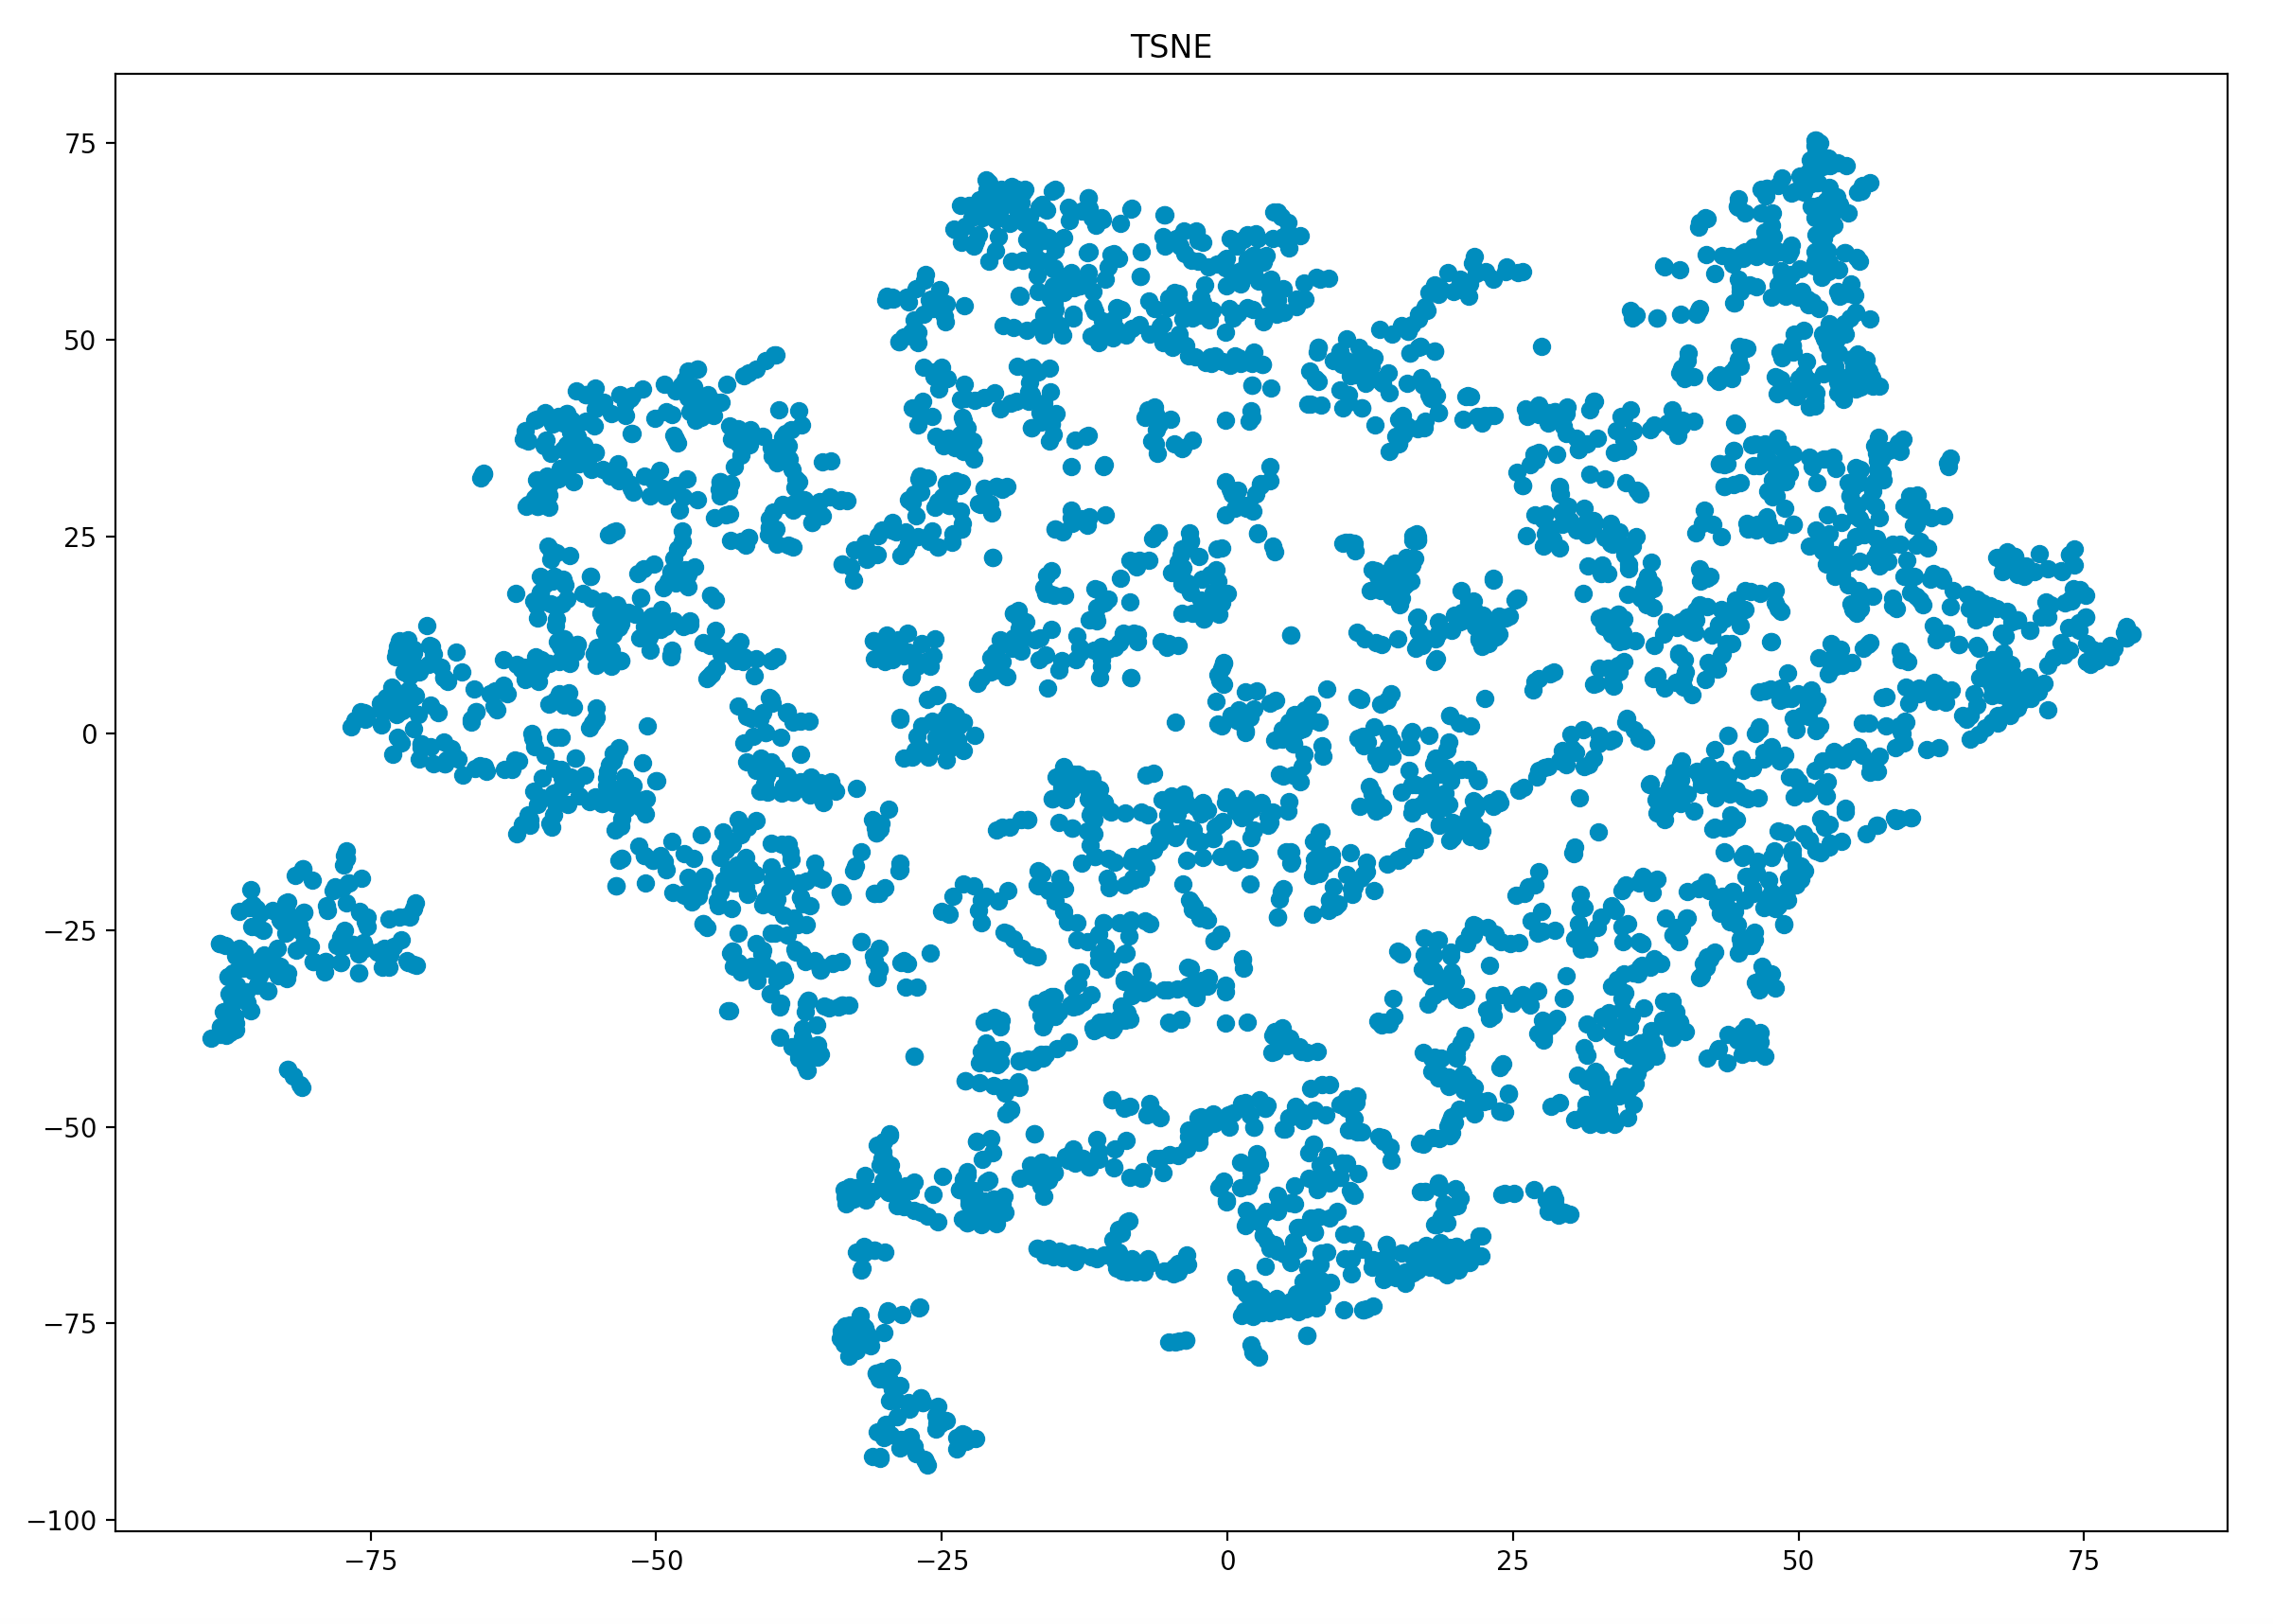
\includegraphics[width=0.9\textwidth]{./images/tsneParametersTest/perplexity/perp30-3hTSNE.png}
  % \caption{}
  % \label{figure:}
  \end{subfigure}%
  \begin{subfigure}{.5\textwidth}
    \centering
    \includegraphics[width=0.9\textwidth]{./images/tsneParametersTest/perplexity/perp30-3hDBSCAN.png}
    % \caption{}
    % \label{figure:}
	\end{subfigure}
	\caption{\textbf{3h} data files, t-SNE calculated with the following parameters: \textbf{perplexity=30}, n\_iter=5000, learning\_rate=50}
  \label{figure:3hperp30TSNE}
\end{figure}



%------------------ PERPLEXITY 40: ------------------
\subsubsection{Perplexity = 40}
% -- 1h, perp 40 --
\begin{figure}[H]
  \centering
  \begin{subfigure}{.5\textwidth}
    \centering
    \includegraphics[width=0.9\textwidth]{./images/tsneParametersTest/perplexity/perp40-1hTSNE.png}
  % \caption{}
  % \label{figure:}
  \end{subfigure}%
  \begin{subfigure}{.5\textwidth}
    \centering
    \includegraphics[width=0.9\textwidth]{./images/tsneParametersTest/perplexity/perp40-1hDBSCAN.png}
    % \caption{}
    % \label{figure:}
  \end{subfigure}
	\caption{\textbf{1h} data files, t-SNE calculated with the following parameters: \textbf{perplexity=40}, n\_iter=5000, learning\_rate=50}
  \label{figure:1hperp40TSNE}
\end{figure}

% -- 3h, perp 40 --
\begin{figure}[H]
  \centering
	\begin{subfigure}{.5\textwidth}
    \centering
    \includegraphics[width=0.9\textwidth]{./images/tsneParametersTest/perplexity/perp40-3hTSNE.png}
  % \caption{}
  % \label{figure:}
  \end{subfigure}%
  \begin{subfigure}{.5\textwidth}
    \centering
    \includegraphics[width=0.9\textwidth]{./images/tsneParametersTest/perplexity/perp40-3hDBSCAN.png}
    % \caption{}
    % \label{figure:}
	\end{subfigure}
	\caption{\textbf{3h} data files, t-SNE calculated with the following parameters: \textbf{perplexity=40}, n\_iter=5000, learning\_rate=50}
  \label{figure:3hperp40TSNE}
\end{figure}



%------------------ PERPLEXITY 45: ------------------
\subsubsection{Perplexity = 45}
% -- 1h, perp 45 --
\begin{figure}[H]
  \centering
  \begin{subfigure}{.5\textwidth}
    \centering
    \includegraphics[width=0.9\textwidth]{./images/tsneParametersTest/perplexity/perp45-1hTSNE.png}
  % \caption{}
  % \label{figure:}
  \end{subfigure}%
  \begin{subfigure}{.5\textwidth}
    \centering
    \includegraphics[width=0.9\textwidth]{./images/tsneParametersTest/perplexity/perp45-1hDBSCAN.png}
    % \caption{}
    % \label{figure:}
  \end{subfigure}
	\caption{\textbf{1h} data files, t-SNE calculated with the following parameters: \textbf{perplexity=45}, n\_iter=5000, learning\_rate=50}
  \label{figure:1hperp45TSNE}
\end{figure}

% -- 3h, perp 45 --
\begin{figure}[H]
  \centering
	\begin{subfigure}{.5\textwidth}
    \centering
    \includegraphics[width=0.9\textwidth]{./images/tsneParametersTest/perplexity/perp45-3hTSNE.png}
  % \caption{}
  % \label{figure:}
  \end{subfigure}%
  \begin{subfigure}{.5\textwidth}
    \centering
    \includegraphics[width=0.9\textwidth]{./images/tsneParametersTest/perplexity/perp45-3hDBSCAN.png}
    % \caption{}
    % \label{figure:}
	\end{subfigure}
	\caption{\textbf{3h} data files, t-SNE calculated with the following parameters: \textbf{perplexity=45}, n\_iter=5000, learning\_rate=50}
  \label{figure:3hperp45TSNE}
\end{figure}



%------------------ PERPLEXITY 50: ------------------
\subsubsection{Perplexity = 50}
% -- 1h, perp 50 --
\begin{figure}[H]
  \centering
  \begin{subfigure}{.5\textwidth}
    \centering
    \includegraphics[width=0.9\textwidth]{./images/tsneParametersTest/perplexity/perp50-1hTSNE.png}
  % \caption{}
  % \label{figure:}
  \end{subfigure}%
  \begin{subfigure}{.5\textwidth}
    \centering
    \includegraphics[width=0.9\textwidth]{./images/tsneParametersTest/perplexity/perp50-1hDBSCAN.png}
    % \caption{}
    % \label{figure:}
  \end{subfigure}
	\caption{\textbf{1h} data files, t-SNE calculated with the following parameters: \textbf{perplexity=50}, n\_iter=5000, learning\_rate=50}
  \label{figure:1hperp50TSNE}
\end{figure}

% -- 3h, perp 50 --
\begin{figure}[H]
  \centering
	\begin{subfigure}{.5\textwidth}
    \centering
    \includegraphics[width=0.9\textwidth]{./images/tsneParametersTest/perplexity/perp50-3hTSNE.png}
  % \caption{}
  % \label{figure:}
  \end{subfigure}%
  \begin{subfigure}{.5\textwidth}
    \centering
    \includegraphics[width=0.9\textwidth]{./images/tsneParametersTest/perplexity/perp50-3hDBSCAN.png}
    % \caption{}
    % \label{figure:}
	\end{subfigure}
	\caption{\textbf{3h} data files, t-SNE calculated with the following parameters: \textbf{perplexity=50}, n\_iter=5000, learning\_rate=50}
  \label{figure:3hperp50TSNE}
\end{figure}





\subsubsection{Perplexity Comparison Results (Average of two different t-SNE runs)}
\label{appendix:compareAveragePerplexity}

\begin{figure}[H]
  \centering
  \includegraphics[width=0.8\textwidth]{./images/tsneParametersTest/perplexity/perplexityEvaluationScoresAverage.png}
  \caption{Comparison of Silhouette Coefficient, Davies-Bouldin Index, and Caliński-Harabasz Index for different t-SNE \textbf{perplexities}. The lighter green highlighted values indicate the best values of that file aggregation (1h or 3h files). The dark green highlighted values illustrate the overall best values over all files (1h and 3h files).}
  \label{figure:perplexityEvaluationScoresAverage}
\end{figure}

\begin{figure}[H]
  \centering
  \includegraphics[width=0.4\textwidth]{./images/tsneParametersTest/perplexity/perplexityEvaluationScoresDetailedAverage.png}
  \caption{Comparison of Silhouette Coefficient, Davies-Bouldin Index, and Caliński-Harabasz Index for different t-SNE \textbf{perplexities}. The lighter green highlighted values indicate the best values of that file aggregation (1h or 3h files). The dark green highlighted values illustrate the overall best values over all files (1h and 3h files).}
  \label{figure:perplexityEvaluationScoresDetailedAverage}
\end{figure}


\clearpage

	\subsection{Learning Rate}
	\label{appendix:tSNEParametersLearningRate}
	
% In the following figures, the t-SNE results of different perplexitites are compared, for the different time length files (1h and 3h), using the first columns of each feature (1h: first 15 minutes, 3h: fist 30 minutes ). The left scatter plots depict t-SNE results, the right scatter plots visualise DBSCAN clusterings of t-SNE results).

%------------------ LEARNING RATE 10: ------------------
\subsubsection{Learning Rate = 10}
% -- 1h, lr 10 --
\begin{figure}[H]
  \centering
  \begin{subfigure}{.5\textwidth}
    \centering
    \includegraphics[width=0.9\textwidth]{./images/tsneParametersTest/learningRate/lr10-1hTSNE.png}
  % \caption{}
  % \label{figure:}
  \end{subfigure}%
  \begin{subfigure}{.5\textwidth}
    \centering
    \includegraphics[width=0.9\textwidth]{./images/tsneParametersTest/learningRate/lr10-1hDBSCAN.png}
    % \caption{}
    % \label{figure:}
  \end{subfigure}
	\caption{\textbf{1h} data files, t-SNE calculated with the following parameters: perplexity=40, n\_iter=5000, \textbf{learning\_rate=10}}
	\label{figure:1hlr10TSNE}
\end{figure}

% -- 3h, lr 10 --
\begin{figure}[H]
	\centering
	
  \centering
	\begin{subfigure}{.5\textwidth}
    \centering
    \includegraphics[width=0.9\textwidth]{./images/tsneParametersTest/learningRate/lr10-3hTSNE.png}
  % \caption{}
  % \label{figure:}
  \end{subfigure}%
  \begin{subfigure}{.5\textwidth}
    \centering
    \includegraphics[width=0.9\textwidth]{./images/tsneParametersTest/learningRate/lr10-3hDBSCAN.png}
    % \caption{}
    % \label{figure:}
	\end{subfigure}
	\caption{\textbf{3h} data files, t-SNE calculated with the following parameters: perplexity=40, n\_iter=5000, \textbf{learning\_rate=10}}
  \label{figure:3hlr10TSNE}
\end{figure}

%------------------ LEARNING RATE 200: ------------------
\subsubsection{Learning Rate = 200}
% -- 1h, lr 200 --
\begin{figure}[H]
  \centering
  \begin{subfigure}{.5\textwidth}
    \centering
    \includegraphics[width=0.9\textwidth]{./images/tsneParametersTest/learningRate/lr200-1hTSNE.png}
  % \caption{}
  % \label{figure:}
  \end{subfigure}%
  \begin{subfigure}{.5\textwidth}
    \centering
    \includegraphics[width=0.9\textwidth]{./images/tsneParametersTest/learningRate/lr200-1hDBSCAN.png}
    % \caption{}
    % \label{figure:}
  \end{subfigure}
	\caption{\textbf{1h} data files, t-SNE calculated with the following parameters: perplexity=40, n\_iter=5000, \textbf{learning\_rate=200}}
	\label{figure:1hlr200TSNE}
\end{figure}

% -- 3h, lr 200 --
\begin{figure}[H]
	\centering
	
  \centering
	\begin{subfigure}{.5\textwidth}
    \centering
    \includegraphics[width=0.9\textwidth]{./images/tsneParametersTest/learningRate/lr200-3hTSNE.png}
  % \caption{}
  % \label{figure:}
  \end{subfigure}%
  \begin{subfigure}{.5\textwidth}
    \centering
    \includegraphics[width=0.9\textwidth]{./images/tsneParametersTest/learningRate/lr200-3hDBSCAN.png}
    % \caption{}
    % \label{figure:}
	\end{subfigure}
	\caption{\textbf{3h} data files, t-SNE calculated with the following parameters: perplexity=40, n\_iter=5000, \textbf{learning\_rate=200}}
  \label{figure:3hlr200TSNE}
\end{figure}


%------------------ LEARNING RATE 400: ------------------
\subsubsection{Learning Rate = 400}
% -- 1h, lr 400 --
\begin{figure}[H]
  \centering
  \begin{subfigure}{.5\textwidth}
    \centering
    \includegraphics[width=0.9\textwidth]{./images/tsneParametersTest/learningRate/lr400-1hTSNE.png}
  % \caption{}
  % \label{figure:}
  \end{subfigure}%
  \begin{subfigure}{.5\textwidth}
    \centering
    \includegraphics[width=0.9\textwidth]{./images/tsneParametersTest/learningRate/lr400-1hDBSCAN.png}
    % \caption{}
    % \label{figure:}
  \end{subfigure}
	\caption{\textbf{1h} data files, t-SNE calculated with the following parameters: perplexity=40, n\_iter=5000, \textbf{learning\_rate=400}}
	\label{figure:1hlr400TSNE}
\end{figure}

% -- 3h, lr 400 --
\begin{figure}[H]
	\centering
	
  \centering
	\begin{subfigure}{.5\textwidth}
    \centering
    \includegraphics[width=0.9\textwidth]{./images/tsneParametersTest/learningRate/lr400-3hTSNE.png}
  % \caption{}
  % \label{figure:}
  \end{subfigure}%
  \begin{subfigure}{.5\textwidth}
    \centering
    \includegraphics[width=0.9\textwidth]{./images/tsneParametersTest/learningRate/lr400-3hDBSCAN.png}
    % \caption{}
    % \label{figure:}
	\end{subfigure}
	\caption{\textbf{3h} data files, t-SNE calculated with the following parameters: perplexity=40, n\_iter=5000, \textbf{learning\_rate=400}}
  \label{figure:3hlr400TSNE}
\end{figure}


%------------------ LEARNING RATE 600: ------------------
\subsubsection{Learning Rate = 600}
% -- 1h, lr 600 --
\begin{figure}[H]
  \centering
  \begin{subfigure}{.5\textwidth}
    \centering
    \includegraphics[width=0.9\textwidth]{./images/tsneParametersTest/learningRate/lr600-1hTSNE.png}
  % \caption{}
  % \label{figure:}
  \end{subfigure}%
  \begin{subfigure}{.5\textwidth}
    \centering
    \includegraphics[width=0.9\textwidth]{./images/tsneParametersTest/learningRate/lr600-1hDBSCAN.png}
    % \caption{}
    % \label{figure:}
  \end{subfigure}
	\caption{\textbf{1h} data files, t-SNE calculated with the following parameters: perplexity=40, n\_iter=5000, \textbf{learning\_rate=600}}
	\label{figure:1hlr600TSNE}
\end{figure}

% -- 3h, lr 600 --
\begin{figure}[H]
	\centering
	
  \centering
	\begin{subfigure}{.5\textwidth}
    \centering
    \includegraphics[width=0.9\textwidth]{./images/tsneParametersTest/learningRate/lr600-3hTSNE.png}
  % \caption{}
  % \label{figure:}
  \end{subfigure}%
  \begin{subfigure}{.5\textwidth}
    \centering
    \includegraphics[width=0.9\textwidth]{./images/tsneParametersTest/learningRate/lr600-3hDBSCAN.png}
    % \caption{}
    % \label{figure:}
	\end{subfigure}
	\caption{\textbf{3h} data files, t-SNE calculated with the following parameters: perplexity=40, n\_iter=5000, \textbf{learning\_rate=600}}
  \label{figure:3hlr600TSNE}
\end{figure}




%------------------ LEARNING RATE 800: ------------------
\subsubsection{Learning Rate = 800}
% -- 1h, lr 800 --
\begin{figure}[H]
  \centering
  \begin{subfigure}{.5\textwidth}
    \centering
    \includegraphics[width=0.9\textwidth]{./images/tsneParametersTest/learningRate/lr800-1hTSNE.png}
  % \caption{}
  % \label{figure:}
  \end{subfigure}%
  \begin{subfigure}{.5\textwidth}
    \centering
    \includegraphics[width=0.9\textwidth]{./images/tsneParametersTest/learningRate/lr800-1hDBSCAN.png}
    % \caption{}
    % \label{figure:}
  \end{subfigure}
	\caption{\textbf{1h} data files, t-SNE calculated with the following parameters: perplexity=40, n\_iter=5000, \textbf{learning\_rate=800}}
	\label{figure:1hlr800TSNE}
\end{figure}

% -- 3h, lr 800 --
\begin{figure}[H]
	\centering
	
  \centering
	\begin{subfigure}{.5\textwidth}
    \centering
    \includegraphics[width=0.9\textwidth]{./images/tsneParametersTest/learningRate/lr800-3hTSNE.png}
  % \caption{}
  % \label{figure:}
  \end{subfigure}%
  \begin{subfigure}{.5\textwidth}
    \centering
    \includegraphics[width=0.9\textwidth]{./images/tsneParametersTest/learningRate/lr800-3hDBSCAN.png}
    % \caption{}
    % \label{figure:}
	\end{subfigure}
	\caption{\textbf{3h} data files, t-SNE calculated with the following parameters: perplexity=40, n\_iter=5000, \textbf{learning\_rate=800}}
  \label{figure:3hlr800TSNE}
\end{figure}


%------------------ LEARNING RATE 1000: ------------------
\subsubsection{Learning Rate = 1000}
% -- 1h, lr 1000 --
\begin{figure}[H]
  \centering
  \begin{subfigure}{.5\textwidth}
    \centering
    \includegraphics[width=0.9\textwidth]{./images/tsneParametersTest/learningRate/lr1000-1hTSNE.png}
  % \caption{}
  % \label{figure:}
  \end{subfigure}%
  \begin{subfigure}{.5\textwidth}
    \centering
    \includegraphics[width=0.9\textwidth]{./images/tsneParametersTest/learningRate/lr1000-1hDBSCAN.png}
    % \caption{}
    % \label{figure:}
  \end{subfigure}
	\caption{\textbf{1h} data files, t-SNE calculated with the following parameters: perplexity=40, n\_iter=5000, \textbf{learning\_rate=1000}}
	\label{figure:1hlr1000TSNE}
\end{figure}

% -- 3h, lr 1000 --
\begin{figure}[H]
	\centering
	
  \centering
	\begin{subfigure}{.5\textwidth}
    \centering
    \includegraphics[width=0.9\textwidth]{./images/tsneParametersTest/learningRate/lr1000-3hTSNE.png}
  % \caption{}
  % \label{figure:}
  \end{subfigure}%
  \begin{subfigure}{.5\textwidth}
    \centering
    \includegraphics[width=0.9\textwidth]{./images/tsneParametersTest/learningRate/lr1000-3hDBSCAN.png}
    % \caption{}
    % \label{figure:}
	\end{subfigure}
	\caption{\textbf{3h} data files, t-SNE calculated with the following parameters: perplexity=40, n\_iter=5000, \textbf{learning\_rate=1000}}
  \label{figure:3hlr1000TSNE}
\end{figure}



\subsubsection{Learning Rate Detailed Comparison Results }
\label{appendix:comparelearningRateDetailed}

\begin{figure}
  \centering
  \includegraphics[width=0.8\textwidth]{./images/tsneParametersTest/learningRate/learningRateEvaluationScoresDetailed.png}
  \caption{Comparison of Silhouette Coefficient, Davies-Bouldin Index, and Caliński-Harabasz Index for different t-SNE \textbf{learning rate} values. Smaller learning rate value steps were taken (i.e. 50, except for the first step which is 40 and the last step to 800) between each test. The lighter green highlighted values indicate the best values of that file aggregation (1h or 3h files). The dark green highlighted values illustrate the overall best values over all files (1h and 3h files).}
  \label{figure:learningRateEvaluationScoresDetailed}
\end{figure}

\begin{figure}
  \centering
  \includegraphics[width=0.8\textwidth]{./images/tsneParametersTest/learningRate/learningRateEvaluationScoresDetailed2.png}
  \caption{Comparison of Silhouette Coefficient, Davies-Bouldin Index, and Caliński-Harabasz Index for different t-SNE \textbf{learning rate} values. Smaller learning rate value steps were taken (i.e. 10, except for the last step to 800) between each test. The lighter green highlighted values indicate the best values of that file aggregation (1h or 3h files). The dark green highlighted values illustrate the overall best values over all files (1h and 3h files).}
  \label{figure:learningRateEvaluationScoresDetailed2}
\end{figure}

%.................................COMPARISON AVERAGES..................................
\subsubsection{Learning Rate Comparison Results (Average of two different t-SNE runs)}
\label{appendix:compareAverageLearningRate}


\begin{figure}[H]
  \centering
  \includegraphics[width=0.8\textwidth]{./images/tsneParametersTest/learningRate/learningRateEvaluationScoresAverage.png}
  \caption{Comparison of Silhouette Coefficient, Davies-Bouldin Index, and Caliński-Harabasz Index for different t-SNE \textbf{learning rate} values, in steps of 200 (except the first step of 190). The lighter green highlighted values indicate the best values of that file aggregation (1h or 3h files). The dark green highlighted values illustrate the overall best values over all files (1h and 3h files).}
  \label{figure:learningRateEvaluationScoresAverage}
\end{figure}

\begin{figure}[H]
  \centering
  \includegraphics[width=0.8\textwidth]{./images/tsneParametersTest/learningRate/learningRateEvaluationScoresAverageDetailed.png}
  \caption{Comparison of Silhouette Coefficient, Davies-Bouldin Index, and Caliński-Harabasz Index for different t-SNE \textbf{learning rate} values. Smaller learning rate value steps were taken (i.e. 50, except for the first step which is 40 and the last step to 800) between each test. The lighter green highlighted values indicate the best values of that file aggregation (1h or 3h files). The dark green highlighted values illustrate the overall best values over all files (1h and 3h files).}
  \label{figure:learningRateEvaluationScoresAverageDetailed}
\end{figure}

\begin{figure}[H]
  \centering
  \includegraphics[width=0.8\textwidth]{./images/tsneParametersTest/learningRate/learningRateEvaluationScoresAverageDetailed2.png}
  \caption{Comparison of Silhouette Coefficient, Davies-Bouldin Index, and Caliński-Harabasz Index for different t-SNE \textbf{learning rate} values. Smaller learning rate value steps were taken (i.e. 10, except for the last step to 800) between each test. The lighter green highlighted values indicate the best values of that file aggregation (1h or 3h files). The dark green highlighted values illustrate the overall best values over all files (1h and 3h files).}
  \label{figure:learningRateEvaluationScoresAverageDetailed2}
\end{figure}

\begin{figure}[H]
  \centering
  \includegraphics[width=0.8\textwidth]{./images/tsneParametersTest/learningRate/learningRateEvaluationScoresAverageDetailed3.png}
  \caption{Comparison of Silhouette Coefficient, Davies-Bouldin Index, and Caliński-Harabasz Index for different t-SNE \textbf{learning rate} values, in steps of 5. The lighter green highlighted values indicate the best values of that file aggregation (1h or 3h files). The dark green highlighted values illustrate the overall best values over all files (1h and 3h files).}
  \label{figure:learningRateEvaluationScoresAverageDetailed3}
\end{figure}






\subsubsection{Learning Rate Comparison of 20 and 800}
\label{appendig:compareLearningRate20and800}

\begin{figure}[H]
  \centering
  \includegraphics[width=1\textwidth]{./images/tsneParametersTest/learningRate/learningRateEvaluationScoresAverageDetailed4.png}
  \caption{Comparison of Silhouette Coefficient, Davies-Bouldin Index, and Caliński-Harabasz Index for the t-SNE \textbf{learning rate} values 20 and 80. The lighter green highlighted values indicate the best values of that file aggregation (1h or 3h files). The dark green highlighted values illustrate the overall best values over all files (1h and 3h files).}
  \label{figure:learningRateEvaluationScoresAverageDetailed4}
\end{figure}

%------------------ 1h: ------------------
\begin{figure}[H]
  \centering
  \begin{subfigure}{.5\textwidth}
    \centering
    \includegraphics[width=0.9\textwidth]{./images/tsneParametersTest/learningRate/lr201h-DBSCANCompare.png}
  % \caption{}
  % \label{figure:}
  \end{subfigure}%
  \begin{subfigure}{.5\textwidth}
    \centering
    \includegraphics[width=0.9\textwidth]{./images/tsneParametersTest/learningRate/lr8001h-DBSCANCompare.png}
    % \caption{}
    % \label{figure:}
  \end{subfigure}
	\caption{\textbf{1h} data files comparison of learning rate: a) 20, b) 800}
	\label{figure:1h-learningRateComparison20and800}
\end{figure}
%------------------ 3h: ------------------
\begin{figure}[H]
  \centering
  \begin{subfigure}{.5\textwidth}
    \centering
    \includegraphics[width=0.9\textwidth]{./images/tsneParametersTest/learningRate/lr203h-DBSCANCompare.png}
  % \caption{}
  % \label{figure:}
  \end{subfigure}%
  \begin{subfigure}{.5\textwidth}
    \centering
    \includegraphics[width=0.9\textwidth]{./images/tsneParametersTest/learningRate/lr8003h-DBSCANCompare.png}
    % \caption{}
    % \label{figure:}
  \end{subfigure}
	\caption{\textbf{3h} data files comparison of learning rate: a) 20, b) 800}
	\label{figure:3h-learningRateComparison20and800}
\end{figure}


\clearpage


\section{Optics reachability plots}
\label{appendix:OPTICSReachabilityPlots}
\begin{figure}[H]
  \centering
  \includegraphics[width=1\textwidth]{./images/OPTICS/1h-1-reachabilityPlot-xi.png}
  \caption{\textbf{1h dataset} (first column - 15 min) OPTICS reachability plot using OPTICS automatic cluster extraction (\textbf{xi}). The coloured bars highlight clusters, whilst the black ones indicate noise.}
  \label{figure:fullSizeReachabilityPlotXi1h}
\end{figure}

\begin{figure}[H]
  \centering
  \includegraphics[width=1\textwidth]{./images/OPTICS/3h-1-reachabilityPlot-xi.png}
  \caption{\textbf{3h dataset} (first column - 30 min) OPTICS reachability plot using OPTICS automatic cluster extraction (\textbf{xi}). The coloured bars highlight clusters, whilst the black ones indicate noise.}
  \label{figure:fullSizeReachabilityPlotXi3h}
\end{figure}



\begin{figure}[H]
  \includegraphics[width=1\textwidth]{./images/OPTICS/1h-1-reachabilityPlot-DBSCAN.png}
  \caption{\textbf{1h dataset} (first column - 15 min) OPTICS reachability plot using \textbf{DBSCAN} clustering. The coloured bars highlight clusters, whilst the black ones indicate noise. The eps parameter, set at 2, his highlighted with a horizontal line.}
  \label{figure:fullSizeReachabilityPlotDBSCAN1h}
\end{figure}

\begin{figure}[H]
  \includegraphics[width=1\textwidth]{./images/OPTICS/3h-1-reachabilityPlot-DBSCAN.png}
  \caption{\textbf{3h dataset} (first column - 30 min) OPTICS reachability plot using \textbf{DBSCAN} clustering. The coloured bars highlight clusters, whilst the black ones indicate noise. The eps parameter, set at 2, his highlighted with a horizontal line.}
  \label{figure:fullSizeReachabilityPlotDBSCAN3h}
\end{figure}




% \begin{figure}[H]
%   \centering
%   \begin{subfigure}{.5\textwidth}\captionsetup{width=.8\linewidth}
%     \centering
%     \includegraphics[width=1\textwidth]{./images/OPTICS/1h-1-reachabilityPlot-xi.png}
%   \caption{1h dataset (first column - 15 min)}
%   \end{subfigure}%
%   \begin{subfigure}{.5\textwidth}\captionsetup{width=.8\linewidth}
%     \centering
%     \includegraphics[width=1\textwidth]{./images/OPTICS/3h-1-reachabilityPlot-xi.png}
%     \caption{3h dataset (first column - 30 min)}
%   \end{subfigure}
%   \caption{OPTICS reachability plot using OPTICS automatic cluster extraction (xi). The coloured bars highlight clusters, whilst the black ones indicate noise.}
%   \label{figure:OPTICSXiResultsReachabilityPlot}
%   \end{figure}



% \begin{figure}[H]
%   \centering
%   \begin{subfigure}{.5\textwidth}\captionsetup{width=.8\linewidth}
%     \centering
%     \includegraphics[width=1\textwidth]{./images/OPTICS/1h-1-reachabilityPlot-DBSCAN.png}
%   \caption{1h dataset (first column - 15 min)}
%   \end{subfigure}%
%   \hfill
%   \begin{subfigure}{.5\textwidth}\captionsetup{width=.8\linewidth}
%     \centering
%     \includegraphics[width=1\textwidth]{./images/OPTICS/3h-1-reachabilityPlot-DBSCAN.png}
%     \caption{3h dataset (first column - 30 min)}
%   \end{subfigure}
%   \caption{OPTICS reachability plot using DBSCAN clustering. The coloured bars highlight clusters, whilst the black ones indicate noise. The eps parameter, set at 2, his highlighted with a horizontal line.}
%   \label{figure:OPTICSResultsReachabilityPlot}
%   \end{figure}


\section{Clustering results}

	\subsection{Clustering scatter plots}
	\label{appendix:clusteringResults}
	\subsubsection{1h aggregated data files}

\begin{figure}[H]
	\centering
	\begin{subfigure}{.5\textwidth}
    \centering
    \includegraphics[width=0.9\textwidth]{./images/clusteringResults/1h-1-DBSCAN.png}
  \end{subfigure}%
  \begin{subfigure}{.5\textwidth}
    \centering
    \includegraphics[width=0.9\textwidth]{./images/clusteringResults/1h-1-OPTICS.png}
	\end{subfigure}
	\caption{Comparison of the scatter plots from the DBSCAN (a) and OPTICS (b) clusterings of the 1st column, so the first \textbf{15 minutes} (1h data files: first 15 minutes).}
  \label{figure:finalClustering1h-1}
\end{figure}

\begin{figure}[H]
	\centering
	\begin{subfigure}{.5\textwidth}
    \centering
    \includegraphics[width=0.9\textwidth]{./images/clusteringResults/1h-2-DBSCAN.png}
  \end{subfigure}%
  \begin{subfigure}{.5\textwidth}
    \centering
    \includegraphics[width=0.9\textwidth]{./images/clusteringResults/1h-2-OPTICS.png}
	\end{subfigure}
	\caption{Comparison of the scatter plots from the DBSCAN (a) and OPTICS (b) clusterings of the average of the 1st column and 2nd column, so the first \textbf{30 minutes} (1h data files: 15 minutes \& 30 minutes).}
  \label{figure:finalClustering1h-2}
\end{figure}

\begin{figure}[H]
	\centering
	\begin{subfigure}{.5\textwidth}
    \centering
    \includegraphics[width=0.9\textwidth]{./images/clusteringResults/1h-3-DBSCAN.png}
  \end{subfigure}%
  \begin{subfigure}{.5\textwidth}
    \centering
    \includegraphics[width=0.9\textwidth]{./images/clusteringResults/1h-3-OPTICS.png}
	\end{subfigure}
	\caption{Comparison of the scatter plots from the DBSCAN (a) and OPTICS (b) clusterings of the average of the 1st column to the 3rd column, so the first \textbf{45 minutes} (1h data files: 15 minutes, 30 minutes \& 45 minutes).}
  \label{figure:finalClustering1h-3}
\end{figure}

\begin{figure}[H]
	\centering
	\begin{subfigure}{.5\textwidth}
    \centering
    \includegraphics[width=0.9\textwidth]{./images/clusteringResults/1h-4-DBSCAN.png}
  \end{subfigure}%
  \begin{subfigure}{.5\textwidth}
    \centering
    \includegraphics[width=0.9\textwidth]{./images/clusteringResults/1h-4-OPTICS.png}
	\end{subfigure}
	\caption{Comparison of the scatter plots from the DBSCAN (a) and OPTICS (b) clusterings of the average of the 1st column to the 4th column, so the whole \textbf{1 hour} (1h data files: 15 minutes, 30 minutes, 45 minutes \& 1 hour).}
  \label{figure:finalClustering1h-4}
\end{figure}









\subsubsection{3h aggregated data files}

\begin{figure}[H]
	\centering
	\begin{subfigure}{.5\textwidth}
    \centering
    \includegraphics[width=0.9\textwidth]{./images/clusteringResults/3h-1-DBSCAN.png}
  \end{subfigure}%
  \begin{subfigure}{.5\textwidth}
    \centering
    \includegraphics[width=0.9\textwidth]{./images/clusteringResults/3h-1-OPTICS.png}
	\end{subfigure}
	\caption{Comparison of the scatter plots from the DBSCAN (a) and OPTICS (b) clusterings of the 1st column, so the first \textbf{30 minutes} (3h data files: first 30 minutes).}
  \label{figure:finalClustering3h-1}
\end{figure}



\begin{figure}[H]
	\centering
	\begin{subfigure}{.5\textwidth}
    \centering
    \includegraphics[width=0.9\textwidth]{./images/clusteringResults/3h-2-DBSCAN.png}
  \end{subfigure}%
  \begin{subfigure}{.5\textwidth}
    \centering
    \includegraphics[width=0.9\textwidth]{./images/clusteringResults/3h-2-OPTICS.png}
	\end{subfigure}
	\caption{Comparison of the scatter plots from the DBSCAN (a) and OPTICS (b) clusterings of the average of the 1st column and 2nd column, so the first \textbf{1 hour} (3h data files: 30 minutes \& 1 hour).}
  \label{figure:finalClustering3h-2}
\end{figure}

\begin{figure}[H]
	\centering
	\begin{subfigure}{.5\textwidth}
    \centering
    \includegraphics[width=0.9\textwidth]{./images/clusteringResults/3h-3-DBSCAN.png}
  \end{subfigure}%
  \begin{subfigure}{.5\textwidth}
    \centering
    \includegraphics[width=0.9\textwidth]{./images/clusteringResults/3h-3-OPTICS.png}
	\end{subfigure}
	\caption{Comparison of the scatter plots from the DBSCAN (a) and OPTICS (b) clusterings of the average of the 1st column to the 3rd column, so the first \textbf{1.5 hours} (3h data files: 30 minutes, 1 hour \& 1 hour 30 minutes).}
  \label{figure:finalClustering3h-3}
\end{figure}

\begin{figure}[H]
	\centering
	\begin{subfigure}{.5\textwidth}
    \centering
    \includegraphics[width=0.9\textwidth]{./images/clusteringResults/3h-4-DBSCAN.png}
  \end{subfigure}%
  \begin{subfigure}{.5\textwidth}
    \centering
    \includegraphics[width=0.9\textwidth]{./images/clusteringResults/3h-4-OPTICS.png}
	\end{subfigure}
	\caption{Comparison of the scatter plots from the DBSCAN (a) and OPTICS (b) clusterings of the average of the 1st column to the 4th column, so the first \textbf{2 hours} (3h data files: 30 minutes, 1 hour, 1 hour 30 minutes \& 2 hours).}
  \label{figure:finalClustering3h-4}
\end{figure}


\begin{figure}[H]
	\centering
	\begin{subfigure}{.5\textwidth}
    \centering
    \includegraphics[width=0.9\textwidth]{./images/clusteringResults/3h-5-DBSCAN.png}
  \end{subfigure}%
  \begin{subfigure}{.5\textwidth}
    \centering
    \includegraphics[width=0.9\textwidth]{./images/clusteringResults/3h-5-OPTICS.png}
	\end{subfigure}
	\caption{Comparison of the scatter plots from the DBSCAN (a) and OPTICS (b) clusterings of the average of the 1st column to the 5th column, so the first \textbf{2.5 hours} (3h data files: 30 minutes, 1 hour, 1 hour 30 minutes, 2 hours \& 2 hours 30 minutes).}
  \label{figure:finalClustering3h-5}
\end{figure}


\begin{figure}[H]
	\centering
	\begin{subfigure}{.5\textwidth}
    \centering
    \includegraphics[width=0.9\textwidth]{./images/clusteringResults/3h-6-DBSCAN.png}
  \end{subfigure}%
  \begin{subfigure}{.5\textwidth}
    \centering
    \includegraphics[width=0.9\textwidth]{./images/clusteringResults/3h-6-OPTICS.png}
	\end{subfigure}
	\caption{Comparison of the scatter plots from the DBSCAN (a) and OPTICS (b) clusterings of the average of the 1st column to the 6th column, so all \textbf{3 hours} (3h data files: 30 minutes, 1 hour, 1 hour 30 minutes, 2 hours, 2 hours 30 minutes \& 3 hours).}
  \label{figure:finalClustering3h-6}
\end{figure}


\clearpage



	\subsection{Clustering evaluation results}
	\label{appendix:clusteringEvaluationResults}
	

\begin{figure}[H]
  \centering
  \includegraphics[width=0.8\textwidth]{./images/clusteringResults/clusteringResults1.png}
  \caption{Evaluation scores comparison from the first 1h run of t-SNE and clustering with a learning rate of 20. The lighter green highlighted values indicate the best values of that file aggregation (1h or 3h files). The dark green highlighted values illustrate the overall best values over all files (1h and 3h files).}
  \label{figure:clusteringResults1}
\end{figure}

\begin{figure}[H]
  \centering
  \includegraphics[width=0.8\textwidth]{./images/clusteringResults/clusteringResults2.png}
  \caption{Evaluation scores comparison from the second 1h run of t-SNE and clustering with a learning rate of 20. The lighter green highlighted values indicate the best values of that file aggregation (1h or 3h files). The dark green highlighted values illustrate the overall best values over all files (1h and 3h files).}
  \label{figure:clusteringResults2}
\end{figure}


\begin{figure}[H]
  \centering
  \includegraphics[width=0.8\textwidth]{./images/clusteringResults/clusteringResults3.png}
  \caption{Evaluation scores comparison averaged from figures \ref{figure:clusteringResults1} and \ref{figure:clusteringResults2}. The lighter green highlighted values indicate the best values of that file aggregation (1h or 3h files). The dark green highlighted values illustrate the overall best values over all files (1h and 3h files).}
  \label{figure:clusteringResults3}
\end{figure}

\begin{figure}[H]
  \centering
  \includegraphics[width=0.8\textwidth]{./images/clusteringResults/clusteringResults4.png}
  \caption{Evaluation scores comparison averaged from 2 runs of t-SNE and clustering with a learning rate of 20. The lighter green highlighted values indicate the best values of that file aggregation (1h or 3h files). The dark green highlighted values illustrate the overall best values over all files (1h and 3h files).}
  \label{figure:clusteringResults4}
\end{figure}

\begin{figure}[H]
  \centering
  \includegraphics[width=0.8\textwidth]{./images/clusteringResults/clusteringResults5.png}
  \caption{Evaluation scores comparison averaged from 2 runs of t-SNE and clustering with a learning rate of 800. The lighter green highlighted values indicate the best values of that file aggregation (1h or 3h files). The dark green highlighted values illustrate the overall best values over all files (1h and 3h files).}
  \label{figure:clusteringResults5}
\end{figure}

\begin{figure}[H]
  \centering
  \includegraphics[width=0.8\textwidth]{./images/clusteringResults/clusteringResultsPlaces.png}
  \caption{Evaluation scores comparison to determine 2nd, 3rd, 4th, 5th, and 6th place.}
  \label{figure:clusterResultsPlaces}
\end{figure}


\clearpage



%\renewcommand{\thesubsection}{\Alph{subsection}}

\section{git-Repository}

% \url{https://gitlab.mediacube.at/fhs41216/BacThesis}


Link to the GitLab Repository on {\url{gitlab.mediacube.at}}:

{\color{red}\url{https://gitlab.mediacube.at/fhs41216/BacThesis}}

\vspace{5mm} %5mm vertical space

\textbf{Git repository contents:}

\begin{itemize}
	\item \textbf{Experiment:} Source code of the experiment
	\item \textbf{Thesis:} LaTeX code of the thesis
	\item \textbf{Literature:} Reference papers available as PDF
	\item \textbf{Websites:} Referenced websites as PDF
	\item \textbf{EvaluationResults:} Excel spreadsheets of cluster evaluation score results
\end{itemize}



\section{Archived Websites}
\label{appendix:archivedWebsites}
% \show\UrlBreaks
\sloppy
\url{https://web.archive.org/web/20200624031033/https://www.anaconda.com/}, snapshot 24.06.2020, 03:10:33

\url{https://web.archive.org/web/20200624072345/https://scikit-learn.org/stable/}, snapshot 24.06.2020, 07:23:45

\url{https://web.archive.org/web/20200626201341/https://matplotlib.org/}, snapshot 26.06.2020, 20:13:41

\url{https://web.archive.org/web/20200624221340/https://developer.android.com/guide/topics/sensors/sensors_motion}, snapshot 24.06.2020, 22:13:40

\url{https://web.archive.org/web/20200620043347/https://tools.ietf.org/html/rfc4180}, snapshot 25.06.2020, 05:29:41

\url{https://web.archive.org/web/20200626201347/https://pandas.pydata.org/}, snapshot 26.06.2020, 20:13:47

\url{https://web.archive.org/web/20200506182431/https://pandas.pydata.org/about/}, snapshot 06.05.2020, 18:24:31

\url{https://web.archive.org/web/20200614223428/https://pandas.pydata.org/pandas-docs/stable/reference/api/pandas.read_csv.html}, snapshot 14.06.2020, 22:34:28

\url{https://web.archive.org/web/20200616004253/https://pandas.pydata.org/pandas-docs/stable/reference/api/pandas.concat.html}, snapshot 16.06.2020, 00:42:53

\url{https://web.archive.org/web/20200608042012/https://pandas.pydata.org/pandas-docs/stable/reference/api/pandas.DataFrame.dropna.html}, snapshot 08.06.2020, 04:20:12

\url{https://web.archive.org/web/20200605104434/https://scikit-learn.org/stable/modules/generated/sklearn.preprocessing.StandardScaler.html}, snapshot 05.06.2020, 10:44:34

\url{https://web.archive.org/web/20200623125839/https://scikit-learn.org/stable/modules/generated/sklearn.decomposition.PCA.html}, snapshot 23.06.2020, 12:58:39

\url{https://web.archive.org/web/20200609055322/https://scikit-learn.org/stable/modules/generated/sklearn.manifold.TSNE.html}, snapshot 09.06.2020, 05:53:22

\url{https://web.archive.org/web/20200623170602/https://distill.pub/2016/misread-tsne/}, snapshot 23.06.2020, 17:06:02

\url{https://web.archive.org/web/20200610080206/https://scikit-learn.org/stable/modules/generated/sklearn.cluster.DBSCAN.html}, snapshot 10.06.2020, 09:17:34

\url{https://web.archive.org/web/20200520193202/https://scikit-learn.org/stable/modules/generated/sklearn.cluster.OPTICS.html}, snapshot 01.06.2020, 07:53:43

\url{https://web.archive.org/web/20200512220200/https://humanstress.ca/stress/understand-your-stress/acute-vs-chronic-stress/}, snapshot 12.05.2020, 22:02:00



\end{appendices}


% group closing
\ifmmtpaper
\endgroup
\fi


\end{document}
